% FH Technikum Wien
% Explizite Kodierung ist nicht normkonform!
%
% Erstellung von Master- und Bachelorarbeiten an der FH Technikum Wien mit Hilfe von LaTeX und der Klasse TWBOOK
%
% Um ein eigenes Dokument zu erstellen, müssen Sie folgendes ergänzen:
% 1) Mit \documentclass[..] einstellen: Master- oder Bachelorarbeit, Studiengang und Sprache
% 2) Mit \newcommand{\FHTWCitationType}.. Zitierstandard festlegen (wird in der Regel vom Studiengang vorgegeben - bitte erfragen)
% 3) Deckblatt, Kurzfassung, etc. ausfüllen
% 4) und die Arbeit schreiben (die verwendeten Literaturquellen in Literatur.bib eintragen)
%
% Getestet mit TeXstudio mit Zeichenkodierung ISO-8859-1 (=ansinew/latin1) und MikTex unter Windows
% Zu beachten ist, dass die Kodierung der Datei mit der Kodierung des paketes inputenc zusammen passt!
% Die Kodierung der Datei twbook.cls MUSS ANSI betragen!
% Bei der Verwendung von UTF8 muss dnicht nur die Kodierung des Dokuments auf UTF8 gestellt sein, sondern auch die des BibTex-Files!
%
% Bugreports und Feedback bitte per E-Mail an latex@technikum-wien.at
%
% Versionen
% *) V0.7: 9.1.2015, RO: Modeline angepasst und verschoben
% *) V0.6: 10.10.2014, RO: Weitere Anpassung an die UK
% *) V0.5: 8.8.2014, WK: Literaturquellen überarbeitet und angepasst
% *) V0.4: 4.8.2014, WK: Initalversion in SVN eingespielt
%
\documentclass[Master,MEE,english]{twbook}%\documentclass[Bachelor,BMR,german]{twbook}
%\usepackage[utf8]{inputenc}
%\usepackage[T1]{fontenc}
\usepackage{fontspec}
\usepackage{microtype}
\usepackage{textcomp}
\usepackage{graphicx}
\usepackage{caption}
\usepackage{subcaption}
\usepackage{pgfplots}
\pgfplotsset{compat=1.10}
\usepackage{pgfplotstable}
\usepackage{siunitx}                       
\usepgfplotslibrary{units}
\usepackage{csquotes}
\usepackage{booktabs}
\usepackage{array}
\usepackage{rotating}
\usepackage{tabularx}
%
% Bitte in der folgenden Zeile den Zitierstandard festlegen
\newcommand{\FHTWCitationType}{HARVARD} % IEEE oder HARVARD möglich - wenn Sie zwischen IEEE und HARVARD wechseln, bitte die temorären Dateien (aux, bbl, ...) löschen
%
\ifthenelse{\equal{\FHTWCitationType}{HARVARD}}{\usepackage{harvard}}{\usepackage{bibgerm}}

% Definition Code-Listings Formatierung:
\usepackage[final]{listings}
\lstset{captionpos=b, numberbychapter=false,caption=\lstname,frame=single, numbers=left, stepnumber=1, numbersep=2pt, xleftmargin=15pt, framexleftmargin=15pt, numberstyle=\tiny, tabsize=3, columns=fixed, basicstyle={\fontfamily{pcr}\selectfont\footnotesize}, keywordstyle=\bfseries, commentstyle={\color[gray]{0.33}\itshape}, stringstyle=\color[gray]{0.25}, breaklines, breakatwhitespace, breakautoindent}
\lstloadlanguages{[ANSI]C, C++, [gnu]make, gnuplot, Matlab}

%Formatieren des Quellcodeverzeichnisses
\makeatletter
% Setzen der Bezeichnungen für das Quellcodeverzeichnis/Abkürzungsverzeichnis in Abhängigkeit von der eingestellten Sprache
\providecommand\listacroname{}
\@ifclasswith{twbook}{english}
{%
    \renewcommand\lstlistingname{Code}
    \renewcommand\lstlistlistingname{List of Code}
    \renewcommand\listacroname{List of Abbreviations}
}{%
    \renewcommand\lstlistingname{Quellcode}
    \renewcommand\lstlistlistingname{Quellcodeverzeichnis}
    \renewcommand\listacroname{Abkürzungsverzeichnis}
}
% Wenn die Option listof=entryprefix gewählt wurde, Definition des Entyprefixes für das Quellcodeverzeichnis. Definition des Macros listoflolentryname analog zu listoflofentryname und listoflotentryname der KOMA-Klasse
\@ifclasswith{scrbook}{listof=entryprefix}
{%
    \newcommand\listoflolentryname\lstlistingname
}{%
}
\makeatother
\newcommand{\listofcode}{\phantomsection\lstlistoflistings}

% Die nachfolgenden 2 Pakete stellen sonst nicht benötigte Features zur Verfügung
%\usepackage{blindtext,dtklogos}

%
% Einträge für Deckblatt, Kurzfassung, etc.
%
\title{Technology comparison and profitability analysis of PV and CSP for large-scale electricity production in South Africa}
\author{Florian Haag, BEng}
\studentnumber{1310578031}
\supervisor{FH-Prof. Dipl.-Ing. Hubert Fechner, MSc, MAS}
\secondsupervisor{Prof. Dr.-Ing. Frank Dinter}
\place{Stellenbosch, South Africa}

\kurzfassung{
Durch steigende Nachfrage bei gleichzeitigen Lieferengpässen benötigt das südafrikanische Elektrizitätssystem derzeit dringend neue Stromerzeugungskapazitäten. Es wird ermittelt, inwieweit solare Stromerzeugung in Engpassfällen eingesetzt werden kann. Hierzu wurden große auf Photovoltaik (PV) basierende Kraftwerke und solarthermische Kraftwerke mit entsprechenden Energiespeichern einander gegenübergestellt. Die solarthermischen Kraftwerke wurden dabei mit einem herkömmlichen, thermischen Energiespeicher ausgestattet. Die Regelbarkeit eines PV-Kraftwerkes durch einen elektrischen Energiespeicher zu ermöglichen, ist außergewöhnlich und wurde bisher in der Praxis nicht umgesetzt. Der Vergleich basiert auf stündlichen Zeitreihensimulationen der solarthermischen Kraftwerke mit thermischen Energiespeichern gegenüber PV-Kraftwerken mit elektrischen Energiespeichern, welche mit variierenden Solarfeldgrößen und Speichervolllaststunden modelliert werden. Dabei basiert der Vergleich der Anlagenleistung auf einer zuvor definierten Ausgangsleistung. Zudem werden die Kraftwerksmodelle nach ihren Stromgestehungskosten untersucht, wobei auch eine Prognose der langfristigen Kostenentwicklung erstellt wird.
}
\schlagworte{Photovoltaik (PV), solarthermisches Kraftwerk, thermische Energiespeicher, elektrische Energiespeicher, Stromgestehungskosten, Kostenentwicklung}
\outline{

%The South African electricity supply has currently a high need for new generation capacity due to rising electricity demand and supply shortages in recent years. It will be discussed how solar energy can support the South African power supply constantly but enhanced due Times of high demand. This thesis compares therefore large-scale photovoltaic (PV) and concentrating solar power (CSP) plants which are equipped with suitable storage applications. For CSP plants a thermal energy storage (TES) is part of the concept and is thereby state of the art. But for large-scale PV power plants is a dispatchability due to a electrical energy storage (EES) more exceptional. The comparison includes hourly time series simulations of a CSP with TES and PV with EES modeling different multiples of solar fields and storage full load hours. The comparison of system performances goes in hands with a specified generation profile for all simulated solar power plants and will also graded by there levelized costs of electricity (LCOE). Furthermore this thesis gives a long-term cost development insight of the main technologies.

The South African electricity system needs new generating capacity due to rising electricity demand and recent supply shortages. The potential for solar energy to provide the necessary capacity during periods of peak demand is investigated. Large-scale photovoltaic (PV) and concentrating solar power (CSP) plants with suitable storage systems are compared. For CSP plants, thermal energy storage (TES), the current state of the art, is used. For large-scale PV power plants, dispatchability through electrical energy storage (EES) is exceptional and has not yet been attempted. The comparison includes hourly time series simulations of a CSP plant with TES and a PV plant with EES, modelled with different solar multiples and storage full load hours. The comparison of system performance for all simulated solar power plants is based on the ability to cover a pre-specified plant output. Performance is also evaluated on the basis of levelized costs of electricity (LCOE). A prognosis of long-term cost evolution is part of the analysis.


}
\keywords{photovoltaic (PV), concentrated solar power (CSP), thermal energy storage (TES), electrical energy storage (EES), levelized cost of electricity (LCOE), cost evolution}
\acknowledgements{
%I wish to express my sincere gratitude, with appreciation, to the supervision of Professor Dr.-Ing. Frank Dinter, Eskom Chair in Concentrating Solar Power (CSP) and Solar Thermal Energy Research Group (STERG) at the Department of Mechanical and Mechatronic Engineering, Stellenbosch University and that of Hubert Fechner, Head of Department at the University of Applied Science, Vienna for there valuable advice and information. 

I wish to express my sincere gratitude to Frank Dinter, Solar Thermal Energy Research Group (STERG) Director and Eskom Chair in Concentrating Solar Power (CSP) in the Department of Mechanical and Mechatronic Engineering, Stellenbosch University and to Hubert Fechner, Head of Department at the FH Technikum University of Applied Sciences, Vienna, with appreciation for their valuable help and advice.

%My Family, especially my Mother Ruth and my deceased Father Karlheinz, I want to thank for always believing in me and supporting me morally and financially during the whole course of my studies. Without them I would not be who and where I am.
Thank you to my friends, especially to Christoph and Philip, who accompanied me during my semester in South Africa, and to everyone who has contributed to my progress throughout my studies.

Finally, I want to thank my family, especially my mother, Ruth, for always believing in me and supporting me morally and financially during the whole course of my studies. You made this achievement possible.

I dedicate this work to my late father, Karlheinz Haag. I am lucky to be his son.
}
% siunitx-Konfiguration
\sisetup{detect-all}
\DeclareSIQualifier\electric{el}
\DeclareSIQualifier\thermal{th}
\DeclareSIQualifier\peak{p}
\DeclareSIQualifier\dc{DC}
\DeclareSIQualifier\ac{AC}
\DeclareSIUnit\wattel{\watt\electric}
\DeclareSIUnit\wattth{\watt\thermal}
\DeclareSIUnit\wattp{\watt\peak}
\DeclareSIUnit\usd{USD}
\DeclareSIUnit\eur{EUR}
\DeclareSIUnit\zar{ZAR}
\DeclareSIUnit\year{a}
\DeclareSIUnit\voltsdc{\volt\dc}
\DeclareSIUnit\voltsac{\volt\ac}
\DeclareSIUnit\ampsdc{\ampere\dc}
\DeclareSIUnit\ampsac{\ampere\ac}
\DeclareSIUnit\wattsdc{\watt\dc}
\DeclareSIUnit\wattsac{\watt\ac}

% KOMA options
\KOMAoption{parskip}{half}
\KOMAoption{appendixprefix}{true}

\setsansfont{Tex Gyre Heros}

\begin{document}

\newcolumntype{C}[1]{>{\centering\arraybackslash}m{#1}} 

%Festlegungen für den HARVARD-Zitierstandard
\ifthenelse{\equal{\FHTWCitationType}{HARVARD}}{
\bibliographystyle{Harvard_FHTW_MR}%Zitierstandard FH Technikum Wien, Studiengang Mechatronik/Robotik, Version 1.2e
\citationstyle{dcu}%Correct citation-style (Harvardand, ";" between citations, "," between author and year)
\citationmode{abbr}%use "et al." with first citation
\iflanguage{ngerman}{
    %Deutsch Neue Rechtschreibung
    \newcommand{\citepic}[1]{(Quelle: \protect\cite{#1})}%Zitat: Bild
    \newcommand{\citefig}[2]{(Quelle: \protect\cite{#1}, S. #2)}%Zitat: Bild aus Dokument
    \newcommand{\citefigm}[2]{(Quelle: modifiziert "ubernommen aus \protect\cite{#1}, S. #2)}%Zitat: modifiziertes Bild aus Dokument
    \newcommand{\citep}{\citeasnoun}%In-Line Zitiat entweder mit \citep{} oder \citeasnoun{}
    \newcommand{\acessedthrough}{Verf{\"u}gbar unter:}%Für URL-Angabe
    \newcommand{\acessedthroughp}{Verf{\"u}gbar bei:}%Für URL-Angabe (Geschützte Datenbank, Zugriff durch FH)
    \newcommand{\acessedat}{Zugang am}%Für URL-Datum-Angabe
    \newcommand{\singlepage}{S.}%Für Seitenangabe (einzelne Seite)
    \newcommand{\multiplepages}{S.}%Für Seitenangabe (mehrere Seiten)
    \newcommand{\chapternr}{K.}%Für Kapitelangabe
    \renewcommand{\harvardand}{\&}%Harvardand in Zitaten
    \newcommand{\abstractonly}{ausschließlich Abstract}
    \newcommand{\edition}{. Auflage}%Angabe der Auflage
}{
\iflanguage{german}{
    %Deutsch
    \newcommand{\citepic}[1]{(Quelle: \protect\cite{#1})}%Zitat: Bild
    \newcommand{\citefig}[2]{(Quelle: \protect\cite{#1}, S. #2)}%Zitat: Bild aus Dokument
    \newcommand{\citefigm}[2]{(Quelle: modifiziert "ubernommen aus \protect\cite{#1}, S. #2)}%Zitat: modifiziertes Bild aus Dokument
    \newcommand{\citep}{\citeasnoun}%In-Line Zitiat entweder mit \citep{} oder \citeasnoun{}
    \newcommand{\acessedthrough}{Verf{\"u}gbar unter:}%Für URL-Angabe
    \newcommand{\acessedthroughp}{Verf{\"u}gbar bei:}%Für URL-Angabe (Geschützte Datenbank, Zugriff durch FH)
    \newcommand{\acessedat}{Zugang am}%Für URL-Datum-Angabe
    \newcommand{\singlepage}{S.}%Für Seitenangabe (einzelne Seite)
    \newcommand{\multiplepages}{S.}%Für Seitenangabe (mehrere Seiten)
    \newcommand{\chapternr}{K.}%Für Kapitelangabe
    \renewcommand{\harvardand}{\&}%Harvardand in Zitaten
    \newcommand{\abstractonly}{ausschließlich Abstract}
    \newcommand{\edition}{. Auflage}%Angabe der Auflage
}{
    %Englisch
    \newcommand{\citepic}[1]{(Source: \protect\cite{#1})}%Zitat: Bild
    \newcommand{\citefig}[2]{(Source: \protect\cite{#1}, p. #2)}%Zitat: Bild aus Dokument
    \newcommand{\citefigm}[2]{(Source: taken with modification from \protect\cite{#1}, p. #2)}%Zitat: modifiziertes Bild aus Dokument
    \newcommand{\citep}{\citeasnoun}%In-Line Zitiat entweder mit \citep{} oder \citeasnoun{}
    \newcommand{\acessedthrough}{Available at:}%Für URL-Angabe
    \newcommand{\acessedthroughp}{Available through:}%Für URL-Angabe (Geschützte Datenbank, Zugriff durch FH)
    \newcommand{\acessedat}{Accessed}%Für URL-Datum-Angabe	
    \newcommand{\singlepage}{p.}%Für Seitenangabe (einzelne Seite)
    \newcommand{\multiplepages}{pp.}%Für Seitenangabe (mehrere Seiten)
    \newcommand{\chapternr}{Ch.}%Für Kapitelangabe
    \renewcommand{\harvardand}{\&}%Harvardand in Zitaten
    \newcommand{\abstractonly}{Abstract only}
    \newcommand{\edition}{~edition}%Edition -> note, that you have to write "edition = {2nd},"!
}}}


\maketitle
%% Einführung 

\renewcommand{\dictumwidth}{0.8\textwidth}
\renewcommand{\dictumauthorformat}[1]{#1}
%\renewcommand{\raggeddictumtext}{\raggedleft}
\renewcommand{\dictumrule}{\vskip1ex\par}
\setkomafont{dictumtext}{\itshape}
\setkomafont{dictumauthor}{\bfseries\upshape}
\cleardoublepage
\thispagestyle{empty}
\begin{minipage}[t]{\textwidth}
\vspace{10cm}
\dictum[Thomas Edison]{We are like tenant farmers chopping down the fence around our house for fuel when we should be using Nature's inexhaustible sources of energy \textemdash sun, wind and tide\textellipsis I'd put my money on the sun and solar energy. What a source of power! I hope we don't have to wait until oil and coal run out before we tackle that.}
\end{minipage}
\cleardoublepage


%% Grundlagen
\mainmatter

\chapter{Introduction}
... % Hier muss noch was hin.

\section{Background and motivation}
%South Africa's energy demand is constantly strong growing while the electricity generation is mainly based on coal, there major resource. Due to growing electricity demand and insufficient investment in the power system in the last decades, led to serious blackouts in late 2005. This forced Eskom Holdings SOC Ltd. (Eskom), the South African public utility, to implement scheduled load shedding during peak hours from 2008 on. The South African electricity supply needs new supporting generation capacities during the day and especially in the evening hours. 

South Africa's energy demand is growing, while electricity generation is mainly based on coal, a major local resource. That growing demand, coupled with insufficient investment in the electrical system in past decades, has led to serious blackouts, beginning in 2005. This forced Eskom Holdings SOC Ltd. (Eskom), the South African public utility, to implement scheduled load shedding during peak hours from 2008 on. The South African electricity supply needs new generation capacity, especially in the evening hours. 

%The high dependency on and the scarcity of fossil resources, the intention to reduce greenhouse gas emissions and other environmental pollutants, rising fuel prices, and the predicted increase of energy demand are also forcing South Africa to promote investments in renewable energy sources. A key section is thereby the high solar radiation in South Africa.

The high dependency on and the scarcity of fossil resources, the intention to reduce greenhouse gas emissions and other environmental pollutants, rising fuel prices, and the predicted increase of energy demand are also forcing South Africa to promote investments in renewable energy sources, among them, solar energy.

Solar radiation may not be used directly. It must first be captured and converted into other forms of energy, primarily heat and electricity. The conversion from solar radiation into electrical energy is by two mechanisms: photovoltaic conversion and thermal conversion. For solar thermal electricity (STE) generation, it is common to concentrate the solar radiation with reflectors onto a receiver where a heat-transfer fluid (HTF) circulates. The fluid is heated up to high temperatures to be used in a thermodynamic cycle to generate electrical power. This technology is called concentrating solar power (CSP). The direct conversion from solar radiation into electricity is based on the photovoltaic effect, using photovoltaic (PV) panels. 

Solar radiation is present only during the daytime. South Africa needs energy over the whole day and especially in the evening hours, when solar radiation is absent. In order to maintain supply, solar plants need energy storage. 

%For CSP power plants storage application are state of the art and can nowerdays assures a constant power generation 24/7. For PV application there are currently large-scale hybrid systems with fossil backup on the marked \cite{BELECTRIC2015} to assure uninterrupted power supply of a PV based system, but pure large-scale PV power plants in connection with energy storage are currently unusual and was before not profound developed. 

For CSP power plants, modern storage systems can assure availability \enquote{24/7}. For photovoltaics, there are currently large-scale hybrid systems with fossil-fueled backup on the market \cite{BELECTRIC2015} to assure uninterrupted supply, but pure large-scale PV power plants in connection with energy storage remain unusual. In this work, large-scale is equivalent to utility-scale.

%It can be expected that plain PV systems are more favourable then CSP systems. But in combination with a energy storage, which is necessary for long duration generation, this situation might be different because of more convenient storage applications of CSP.

Photovoltaic systems are technologically simpler than concentrating solar power systems. When combined with energy storage, however, the choice is not so clear; CSP systems have storage options which can be more attractive, both from an operational and financial perspective.

%This thesis provides therefore a comparison of large-scale solar power plants to support the South African power supply constantly and enhanced on high demand times.

\section{Objective of this thesis}
%The objective of this thesis is the technical and economic comparison of concentrating solar and photovoltaic power plants and the most reasonable storage systems for both technologies. This comparison is limited to South Africa and there specified needs in power generation.

The objective of this thesis is the technical and economic comparison of concentrating solar and photovoltaic power plants, and the evaluation of storage systems for both technologies. This comparison is limited to South Africa under consideration of its specific circumstances and requirements.

A cost prognosis is also considered, in order to provide infrastructure planning guidance.

The research question is as follows:
\begin{quote}
%Which technology, concentrating solar or photovoltaic power plants, in combination with suitable storage systems, will prevail in South Africa in a technical and economical comparison? What is the forecasted cost development of these technologies in the medium- and long-term?
Which technology, concentrating solar or photovoltaic power plants, in combination with suitable storage systems, will prevail in South Africa in a technical and economical comparison? What is the predicted cost development of these technologies in the medium- and long-term?
\end{quote}


\section{Approach}

This thesis follows a bottom-up design, meaning that all essential information is to be found at the beginning of the study.

%The first step of this work is to describe the power supply situation in South Africa from there demand over the generation and distribution to there major supply problems. Thereby the reader gets a impression of the need in South Africa for constant, but flexible power generation.

The basis for the analysis is a study of the electric power sector in South Africa, from demand, to generation, to distribution, to the country's serious supply problems. The reader should understand the need in South Africa for consistent but flexible power generation.

%The second step is to describe the special solar irradiation situation in South Africa and the located potential for generating power from solar power plants. This will also reveal the downside of  direct solar generation without provide energy in storage for the South African electricity supply structure and thereby the need for storage application of solar power plants. A generation profile for the solar power plants will be defined to support the South African power supply at any time of the day but with a main focus on times with high demand. 

Next, the special solar irradiation characteristics of South Africa are considered and described in detail, in order to show the potential, if any, for generating electricity from solar power plants. Disadvantages of direct solar generation will be highlighted, paying particular attention to lack of night generation in the absence of storage. A model plant output profile will be defined for the purpose of supporting the South African electrical system at any time of day, while paying particular attention to peak demand periods.

%The next step is to describe the currently commercial and mature situation of solar power generation and there individual suitable storage technology. Thereby the exact technology type for the comparison will be selected. In order to compare the solar power plants equally they will be simulated under same conditions and requirements (location, weather data and generation profile) by using the System Advisor Model (SAM) software from the National Renewable Energy Laboratory (NREL) \cite{NREL2015}. SAM is designed to model and simulate performance and financial parameter of different types of renewable energy. It also can model PV and CSP application with belonging storage applications. The solar power plant will be modeled and simulated individually and compared in the following. The main performance and financial metrics for the comparison will be the amount of covering of the generation profile and the resulting LCOE.

After a survey of the state of the art, technologies used in the comparison will be chosen. To make the comparison fair, the model plants will be simulated under the same conditions and requirements (location, weather data and generation profile) using the System Advisor Model (SAM) software from the National Renewable Energy Laboratory (NREL) \cite{NREL2015}. SAM is designed to model and simulate performance and produce financial projections for different types of renewable energy. It can model PV and CSP applications with attached storage. The solar power plant will be modelled and simulated individually, then compared. The main performance and financial metrics for the comparison will be the output profile coverage and the resulting levelized cost of electricity.

%At the end the future cost development of the solar power plants will be discussed and compared with new-built conventional power plant costs in South Africa.

Finally, the future cost development of the solar power plants will be discussed and compared with new-build conventional power plant costs in South Africa.

\section{Sources}
In order to assure a academic work with high quality standard, all of the information and data used in this study were gathered from scientific publications or databases, renowned institutions/departments and libraries.

The following sources were considered to obtain scientific provable information:
%\begin{itemize}
%\item Solar Thermal Energy Research Group (STERG)
%\item Centre for Renewable and Sustainable Energy Studies (CRSES)
%\item Library of Stellenbosch University
%\item Library of FH Technikum Wien (University of Applied Science Vienna)
%\item Library of TU Munich
%\item Library of Science Direct
%\end{itemize}
\begin{itemize}
\item Solar Thermal Energy Research Group (STERG)
\item Centre for Renewable and Sustainable Energy Studies (CRSES)
\item Stellenbosch University Library
\item FH Technikum Wien (University of Applied Science Vienna) Library
\item TU Munich Library
\item Elsevier ScienceDirect
\end{itemize}

%Further information was mainly obtained from Eskom, the Department of Energy (DoE), NREL, BP and the International Energy Agency (IEA).

Further information was mainly obtained from Eskom, the Department of Energy of the Republic of South Africa (DoE), the US National Renewable Energy Laboratory (NREL), BP plc and the International Energy Agency (IEA).

%To assure a high quality of this academic work, all units are described in SI units system and applied after the current state of art \cite{Blankenburg2011}.

All units are SI units.
%\chapter{Methods}

%In order to assure a clearly and comprehensible approach this thesis follows a bottom-up design. Therefore all reasonable information are to find at the beginning of the study. The general approach and the information procurement are described in the following.

This thesis follows a bottom-up design, meaning that all essential information is to be found at the beginning of the study.

\section{Approach}
%The first step of this work is to describe the power supply situation in South Africa from there demand over the generation and distribution to there major supply problems. Thereby the reader gets a impression of the need in South Africa for constant, but flexible power generation.

The basis for the analysis is a study of the electric power sector in South Africa, from demand, to generation, to distribution, to the country's serious supply problems. The reader should understand the need in South Africa for consistent but flexible power generation.

%The second step is to describe the special solar irradiation situation in South Africa and the located potential for generating power from solar power plants. This will also reveal the downside of  direct solar generation without provide energy in storage for the South African electricity supply structure and thereby the need for storage application of solar power plants. A generation profile for the solar power plants will be defined to support the South African power supply at any time of the day but with a main focus on times with high demand. 

Next, the special solar irradiation characteristics of South Africa are considered and described in detail, in order to show the potential, if any, for generating electricity from solar power plants. Disadvantages of direct solar generation will be highlighted, paying particular attention to lack of night generation in the absence of storage. A model plant output profile will be defined for the purpose of supporting the South African electrical system at any time of day, while paying particular attention to peak demand periods.

%The next step is to describe the currently commercial and mature situation of solar power generation and there individual suitable storage technology. Thereby the exact technology type for the comparison will be selected. In order to compare the solar power plants equally they will be simulated under same conditions and requirements (location, weather data and generation profile) by using the System Advisor Model (SAM) software from the National Renewable Energy Laboratory (NREL) \cite{NREL2015}. SAM is designed to model and simulate performance and financial parameter of different types of renewable energy. It also can model PV and CSP application with belonging storage applications. The solar power plant will be modeled and simulated individually and compared in the following. The main performance and financial metrics for the comparison will be the amount of covering of the generation profile and the resulting LCOE.

After a survey of the state of the art, technologies used in the comparison will be chosen. To make the comparison fair, the model plants will be simulated under the same conditions and requirements (location, weather data and generation profile) using the System Advisor Model (SAM) software from the National Renewable Energy Laboratory (NREL) \cite{NREL2015}. SAM is designed to model and simulate performance and produce financial projections for different types of renewable energy. It can model PV and CSP applications with attached storage. The solar power plant will be modelled and simulated individually, then compared. The main performance and financial metrics for the comparison will be the output profile coverage and the resulting levelized cost of electricity.

%At the end the future cost development of the solar power plants will be discussed and compared with new-built conventional power plant costs in South Africa.

Finally, the future cost development of the solar power plants will be discussed and compared with new-build conventional power plant costs in South Africa.

\section{Sources}
In order to assure a academic work with high quality standard, all of the information and data used in this study were gathered from scientific publications or databases, renowned institutions/departments and libraries.

The following sources were considered to obtain scientific provable information:
%\begin{itemize}
%\item Solar Thermal Energy Research Group (STERG)
%\item Centre for Renewable and Sustainable Energy Studies (CRSES)
%\item Library of Stellenbosch University
%\item Library of FH Technikum Wien (University of Applied Science Vienna)
%\item Library of TU Munich
%\item Library of Science Direct
%\end{itemize}
\begin{itemize}
\item Solar Thermal Energy Research Group (STERG)
\item Centre for Renewable and Sustainable Energy Studies (CRSES)
\item Stellenbosch University Library
\item FH Technikum Wien (University of Applied Science Vienna) Library
\item TU Munich Library
\item Elsevier ScienceDirect
\end{itemize}

%Further information was mainly obtained from Eskom, the Department of Energy (DoE), NREL, BP and the International Energy Agency (IEA).

Further information was mainly obtained from Eskom, the Department of Energy of the Republic of South Africa (DoE), the US National Renewable Energy Laboratory (NREL), BP plc and the International Energy Agency (IEA).

%To assure a high quality of this academic work, all units are described in SI units system and applied after the current state of art \cite{Blankenburg2011}.

All units are SI units.





\chapter{The South African energy sector}
The Republic of South Africa (SA) is one of the most developed country in Sub-Saharan Africa and acording to the Human Development Index (HDI) it is growing constand since the 1980's, nevertheless it counts as medium developed country \cite{UNDP2014}. Also the population and energy demand is constantly growing \cite{TheWorldBank2015,Agency2015}.

SA has also one of the strongest econemys in Africa, therfore it is accounting for about 30~\% of the primary energy consumption of the entire continent Africa in 2014 \cite{BP2015b}. 
\section{Primary energy consumption}
\begin{figure}[!b]
        \centering                
        \begin{subfigure}[b]{0.45\textwidth}
                \centering
                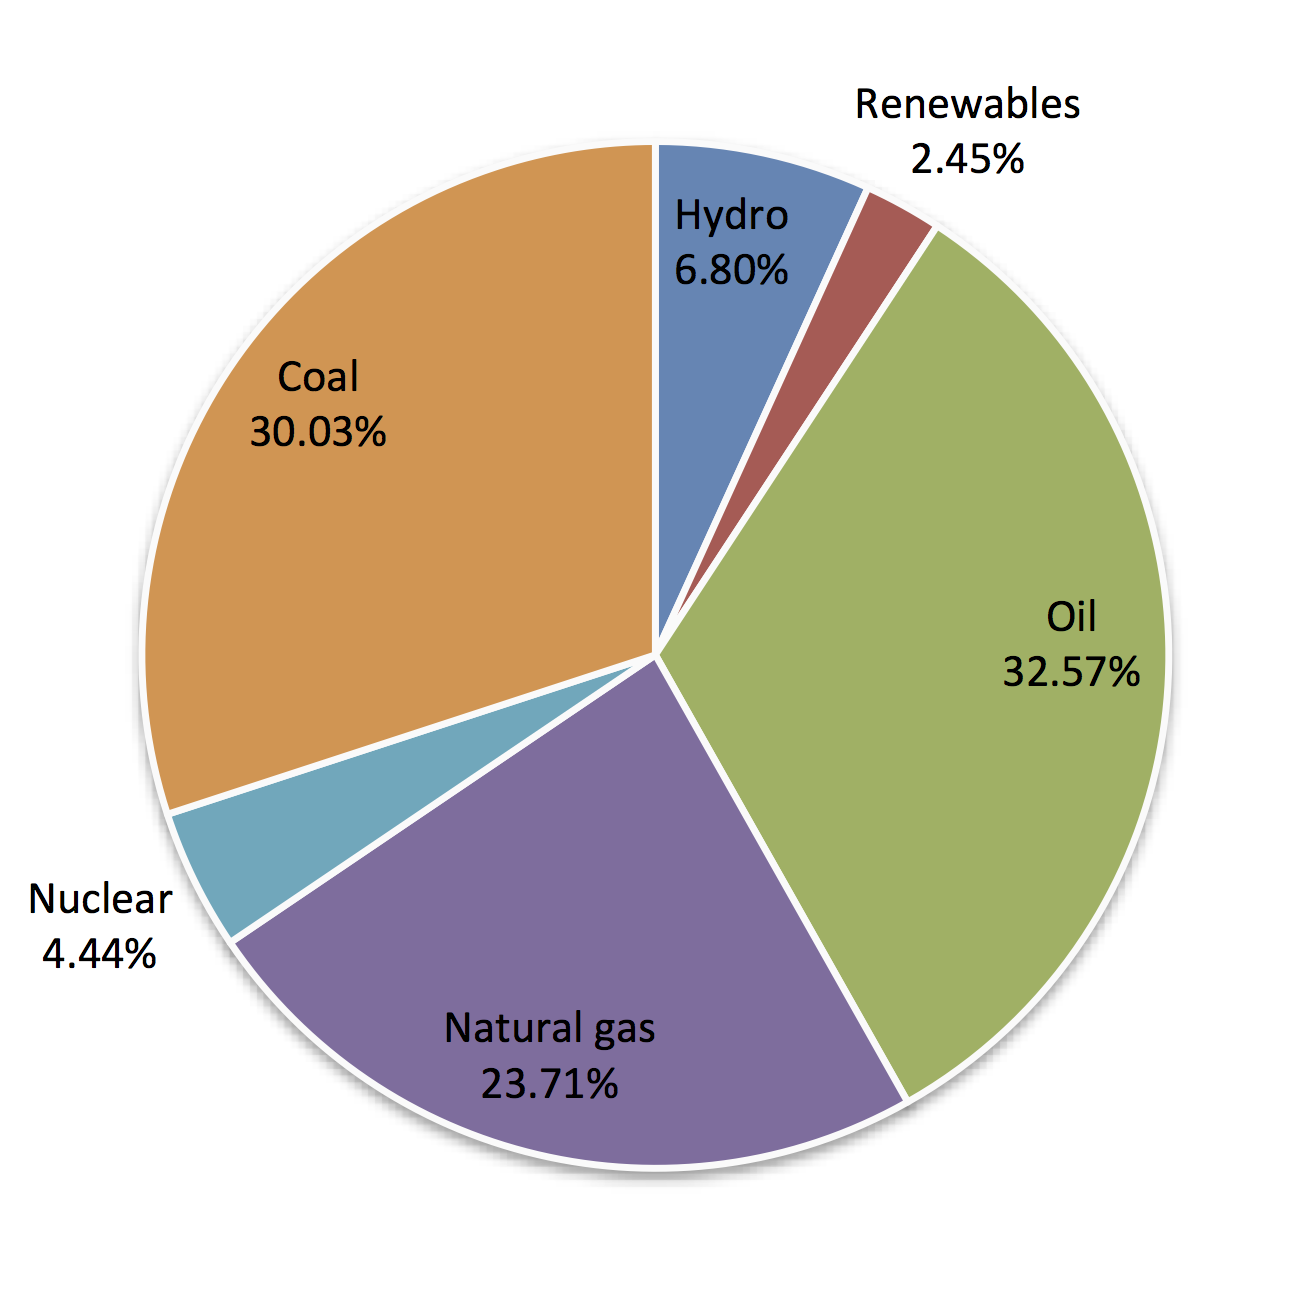
\includegraphics[width=1\textwidth]{FIG/PrimWorld}
                \caption{World share of primary energy consuption.}\label{PrimWorld}
        \end{subfigure}
        ~
        \begin{subfigure}[b]{0.45\textwidth}
                \centering
                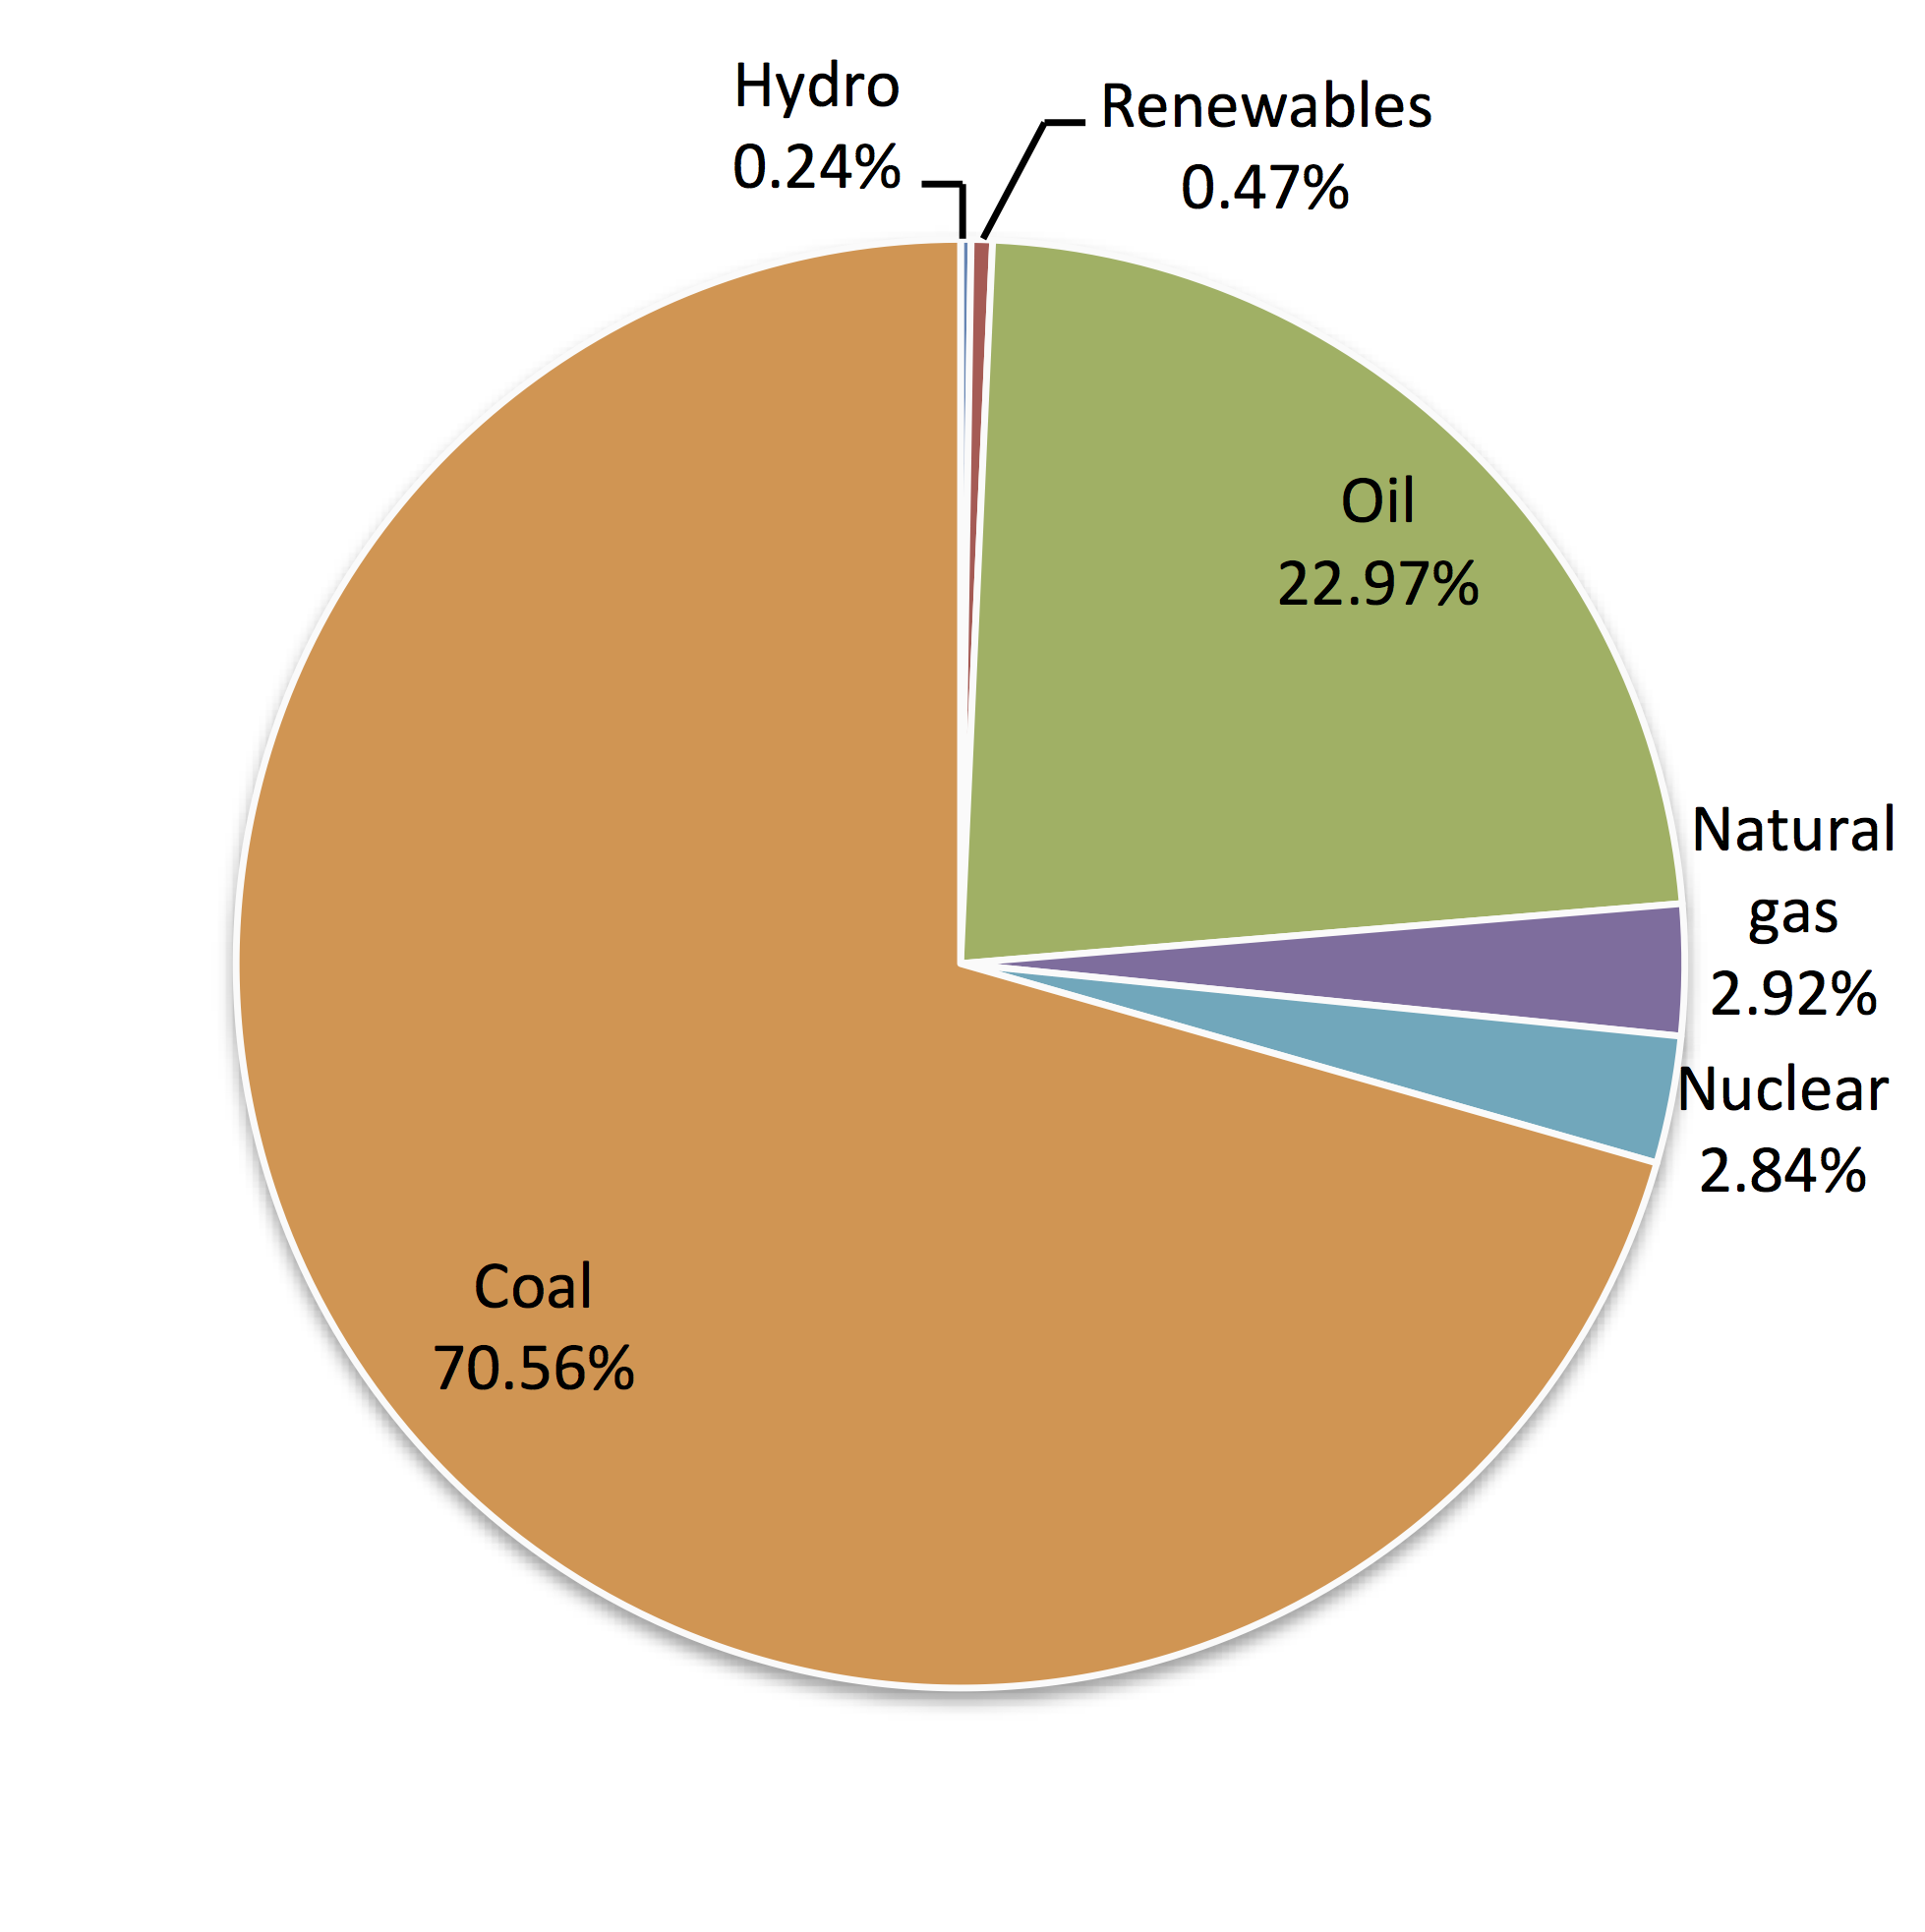
\includegraphics[width=1\textwidth]{FIG/PrimSA}
                \caption{SA share of primary energy consuption.}\label{PrimSA}
        \end{subfigure}
\caption[Comparision of Worldwide and South African primary energy consumption by fuel in 2014.]{Comparision of Worldwide and South African primary energy consumption by fuel in 2014 \cite{BP2015b}.}\label{PEKreis}
\end{figure}
The primary energy consumption of SA was in 2014 about 1~473.52~TWh \cite{BP2015b}. This consumption is mainly based on fossil energy resources. More than 96~\% of the primary energy consumption was in 2014 based fossil fuels and further 2.8~\% on nuclear. Thereby is the share on primary energy consumption predominant coming from coal. Figure \ref{PEKreis} shows the primary energy mix of SA in comparision with the worldwide primary energy mix. \cite{BP2015b}

It can be seen that coal is with about 71~\% the main primary energy source. Also crude oil (23~\%) is a very important energy source for SA. Therefor is the primary energy consumption from renewable energies in SA just about 0.7~\%. Comparing to this, the global share of  renewable primary energy consumption was about 9.3~\% in 2015. But it must be said that the share on renewable energy growth by 482.2 \% from 2013 to 2014. \cite{BP2015b}

Figure \ref{PrimEnergyDevelopment} shows the growing South African primary energy consumption. Between 1965 and 2014 the annual primary energy consumption in SA has risen from 351.96~TWh up to 1~473.52~TWh. Consequently a avarage anual growing rate in primary energy consumption in SA of 8.5~\% in the past half century. \cite{BP2015c}

\begin{figure}[htbp]  
\centering
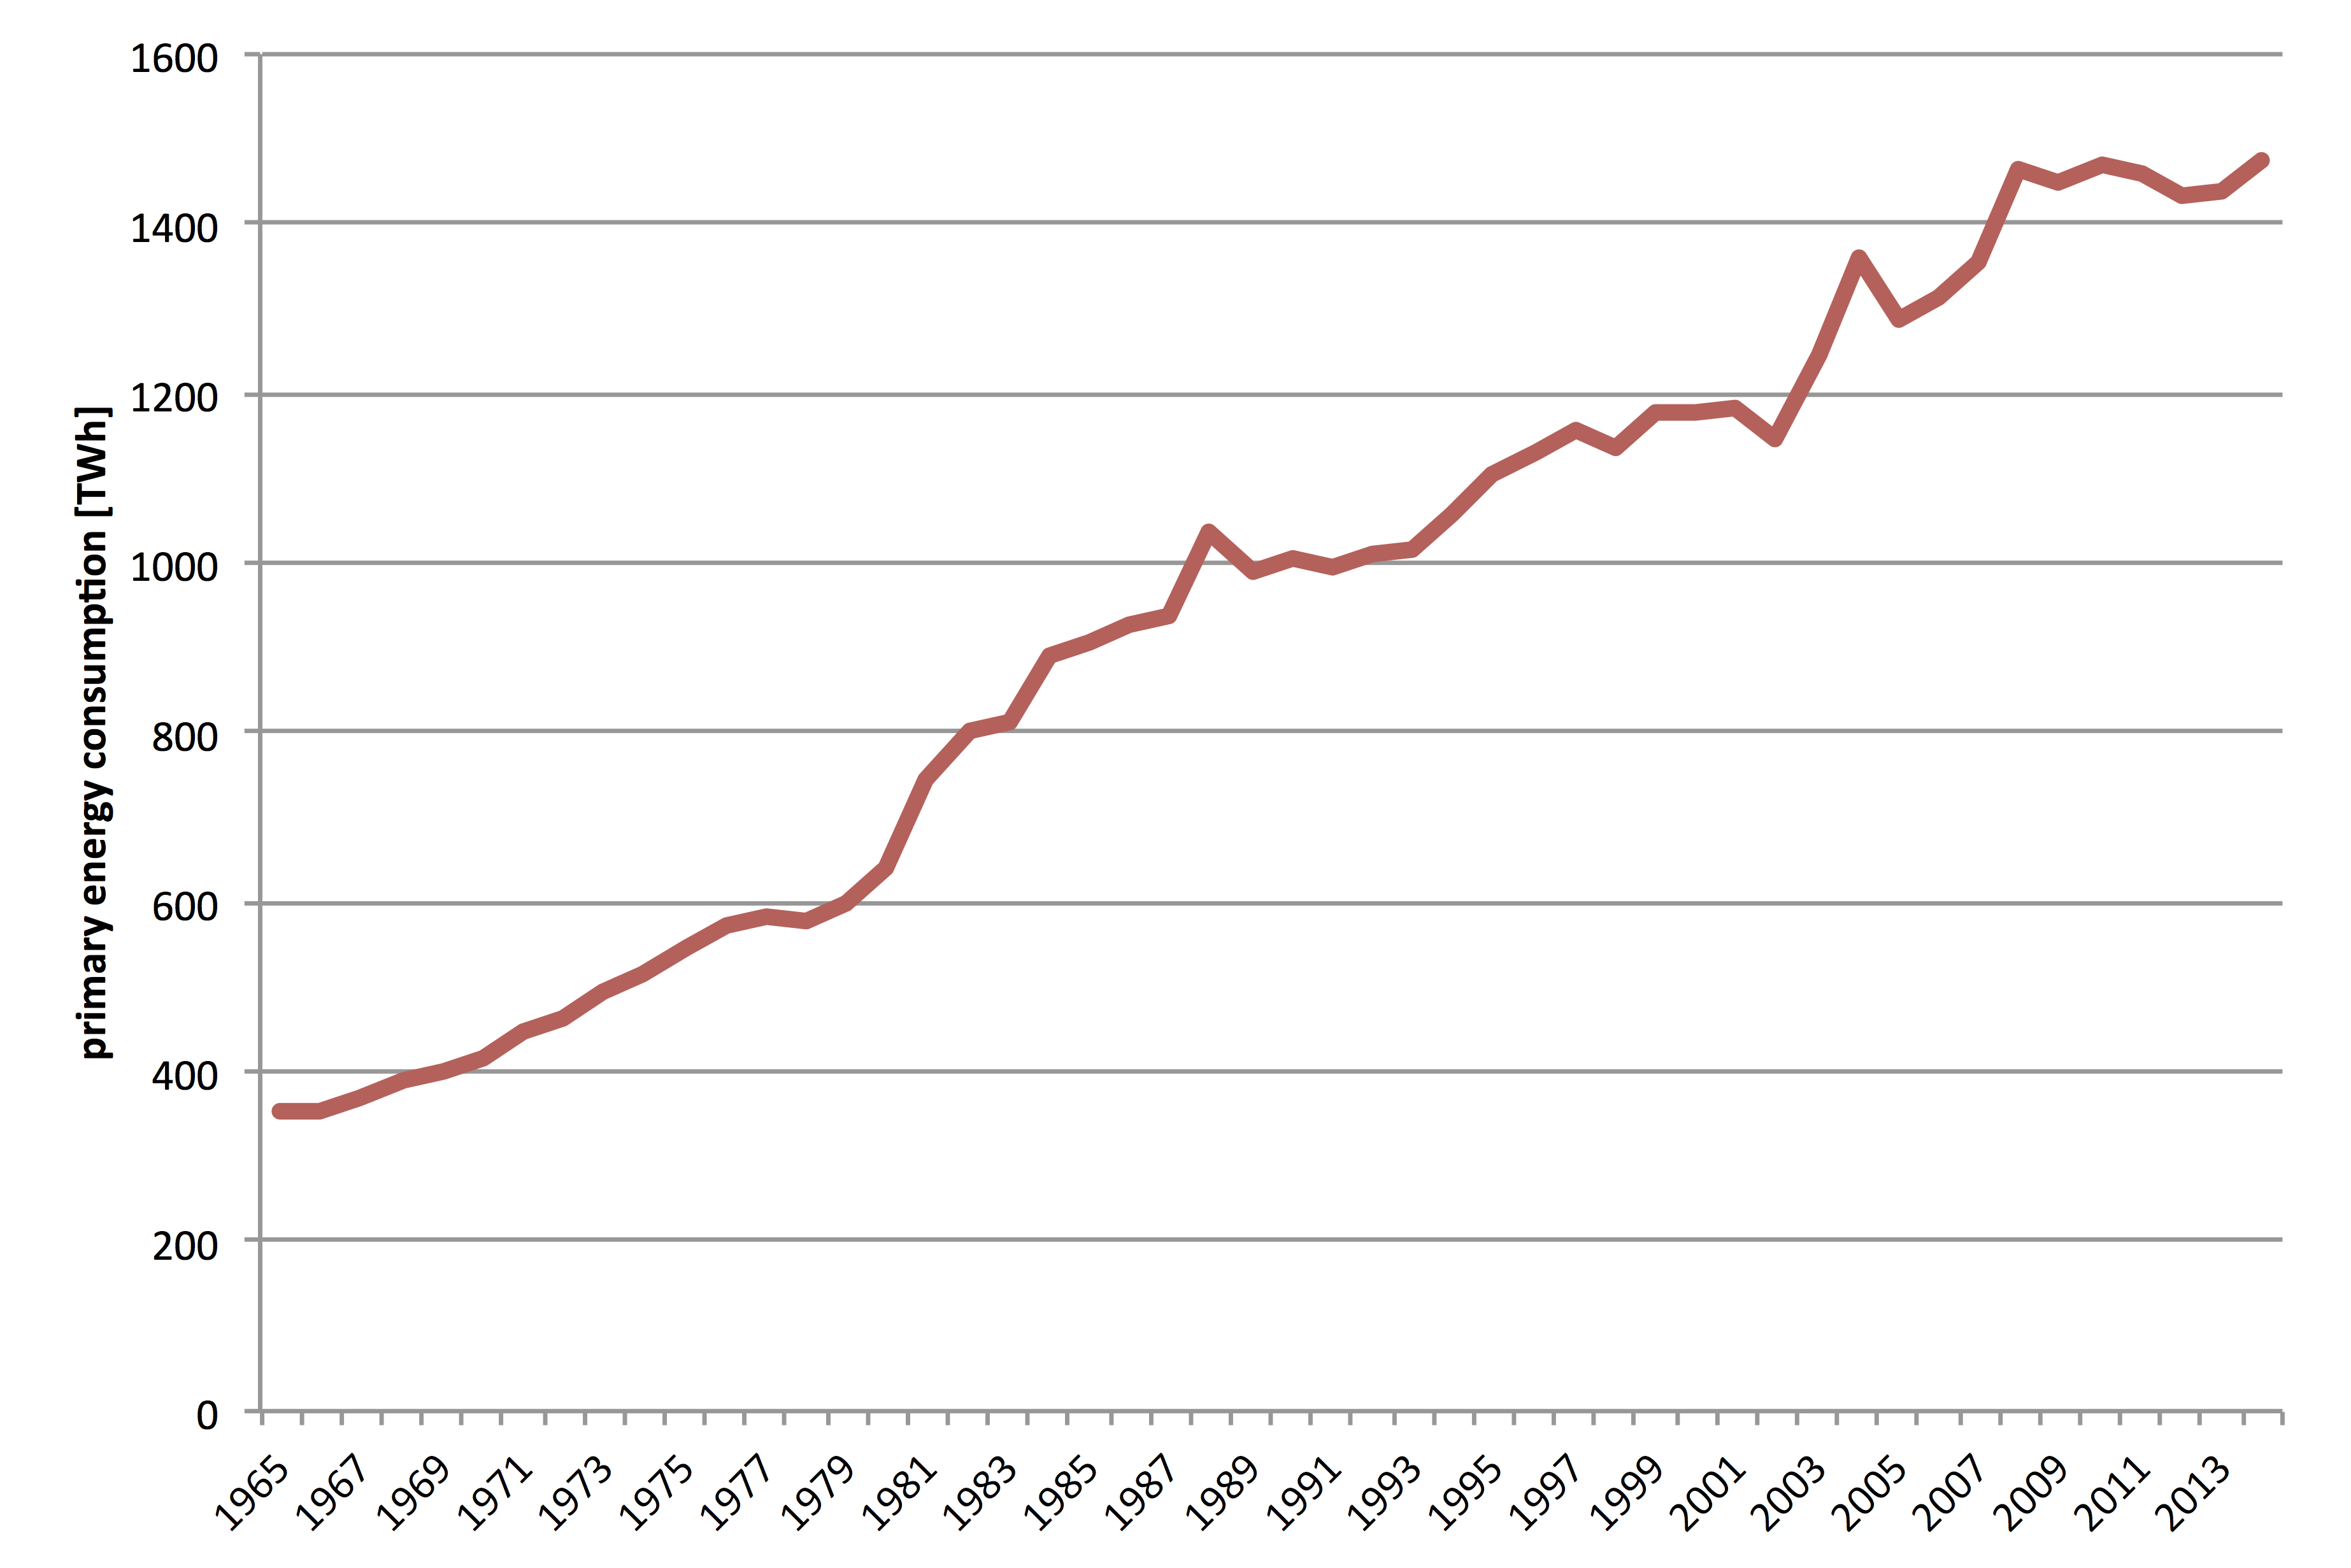
\includegraphics[width=1\linewidth]{FIG/PrimEnergyDevelopment}
\caption[Evolution of primary energy consuption of SA.]{Evolution of primary energy consuption of SA \cite{BP2015c}.}\label{PrimEnergyDevelopment}
\end{figure}
The spread in consumption of primary energy is defined by three major consumption groups, namly the industry sector with about 34.9~\%, the transport sector which consumes about 28.6~\% and other sectors with about 36.5~\%, which includes agriculture, commerce and public services, residential and non-specified consumers \cite{DepartmentofEnergy2012}. So it can be said that the sectors industy and transport are the main energy consumer in SA. 
\pagebreak
\section{Electricity supply and demand}
Coal-fired power stations restrained the electricity generation in SA. 92.8~\% was generated thought coal (239~344~GWh) in 2012, while 5.1~\% of the annual supply was generated by nuclear power (13~075~GWh) and 1.3~\% was generated from hydropower applications (4~860~GWh). Less significant electricity sources for SA are 0.08~\% Oil (194~GWh), 0.11~\% bio-fuels (293~GWh), 0.02~\% PV (50~GWh) and 0.04~\% wind (103~GWh). \cite{Agency2015}



The final electricity consumption in SA was about 197~092~GWh in 2012. The final consumption consist also three main consumers. The largest consumer group with about 59.5~\% are industrial consumers, followed by residential consumers (19.7~\%) and commercial and public services (14.3~\%). The complete electricity flow is shown in Annexure I, Part A, Table \ref{tab1}, on page \pageref{tab1}. \cite{Agency2015}

\begin{figure}[!h] % Sommer/Winter Verbrauchskurve
\centering
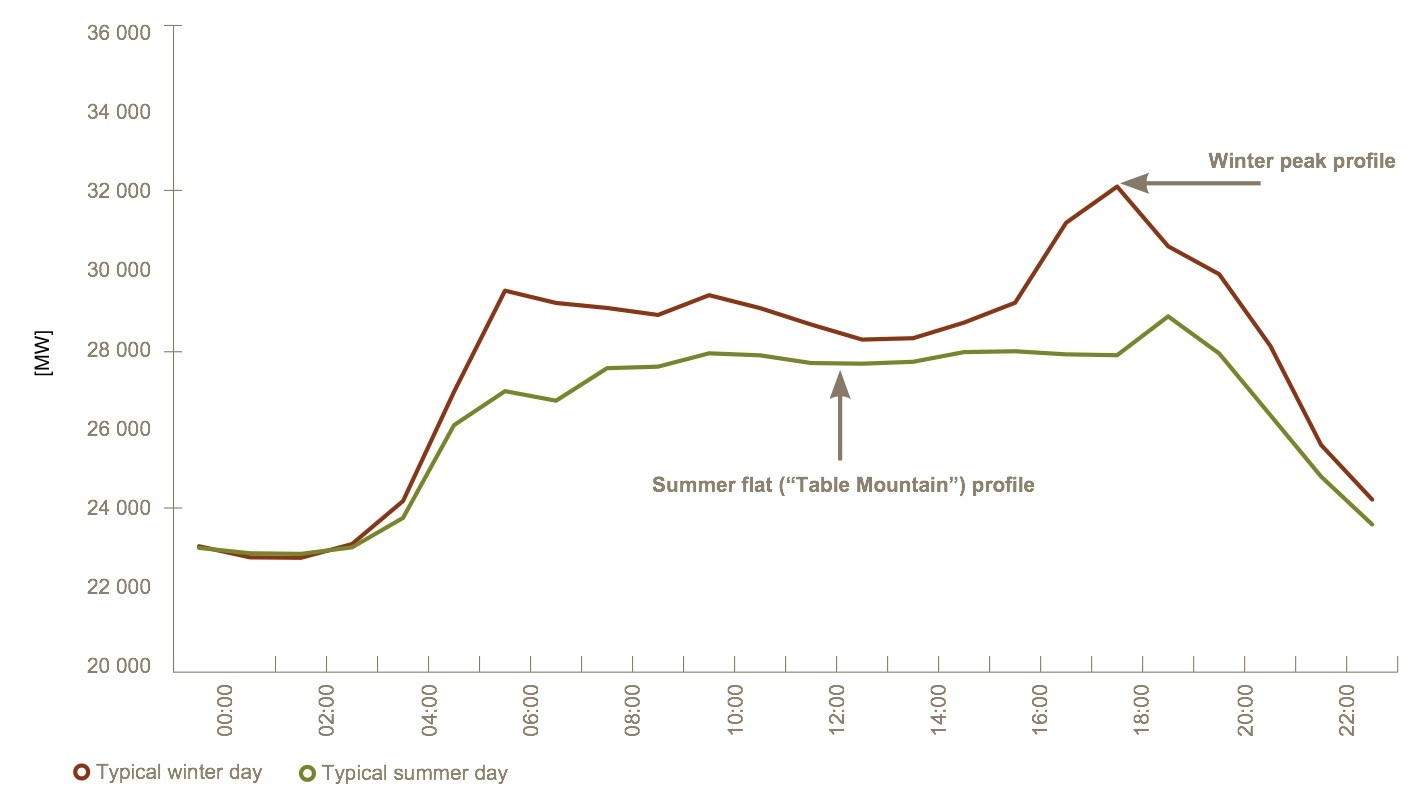
\includegraphics[width=0.9\linewidth]{FIG/SummerWinterDemand}
\caption[Summer and winter load profiles.]{Summer and winter load profiles \cite{Eskom2014}.}\label{DEMAND}
\end{figure}


The demand in South Africa has different load profiles during winter and summer as shown in Figure~\ref{DEMAND}. The peak demand is usually in the evening hours and particularly high during winter time. According to Eskom is the peak demand at about 32~GW, while the usually demand during daytime is between 26~GW and 29~GW. \cite{Eskom2014}

\subsection{Rising energy consumption and security of supply}

\begin{figure}[!h] % Monthly Reserve
\centering
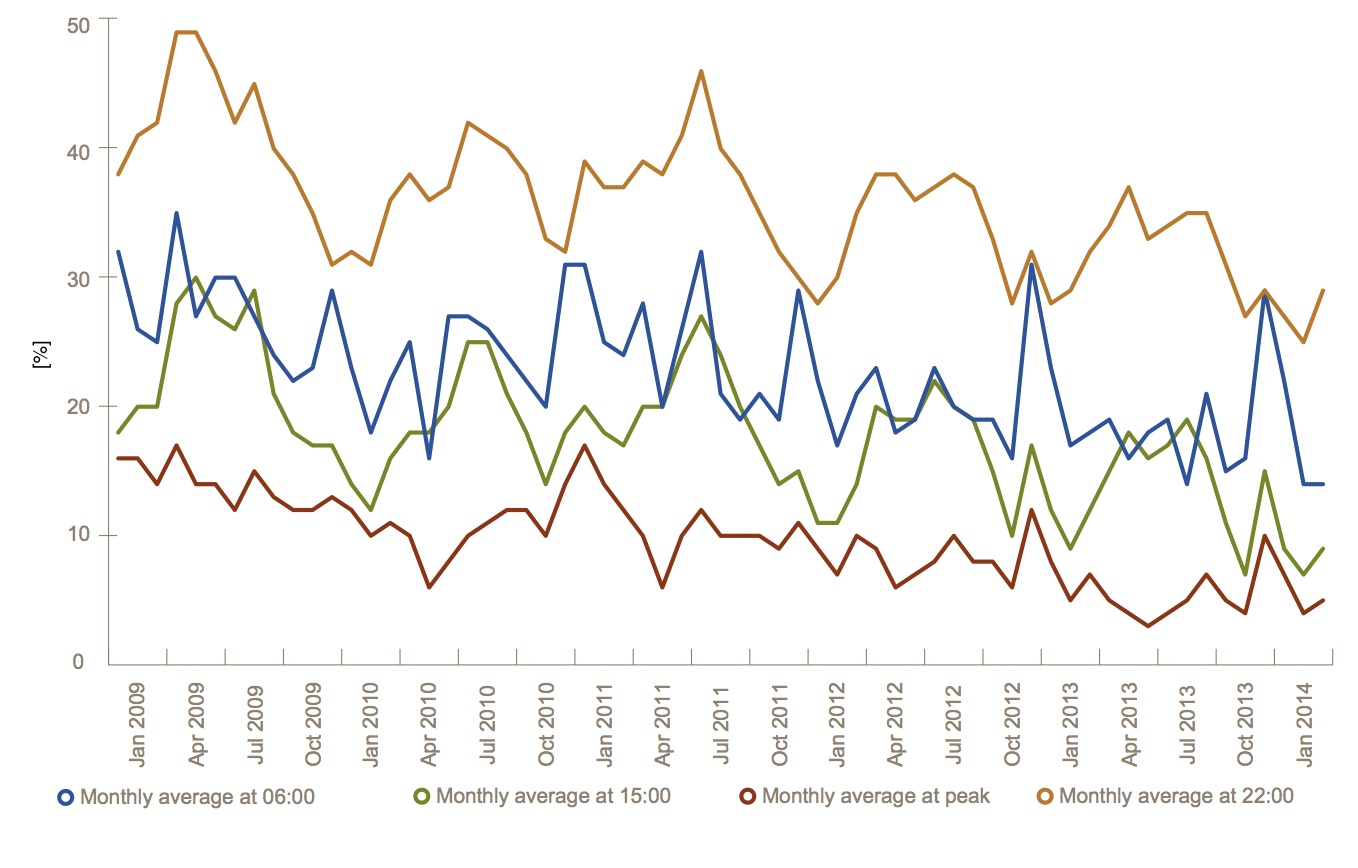
\includegraphics[width=0.9\linewidth]{FIG/AveragemonthlySA}
\caption[Average monthly \% operating reserves.]{Average monthly \% operating reserves\cite{Eskom2014}.}\label{Abb1}
\end{figure}


\begin{figure}[!h] % Demand growth
\centering
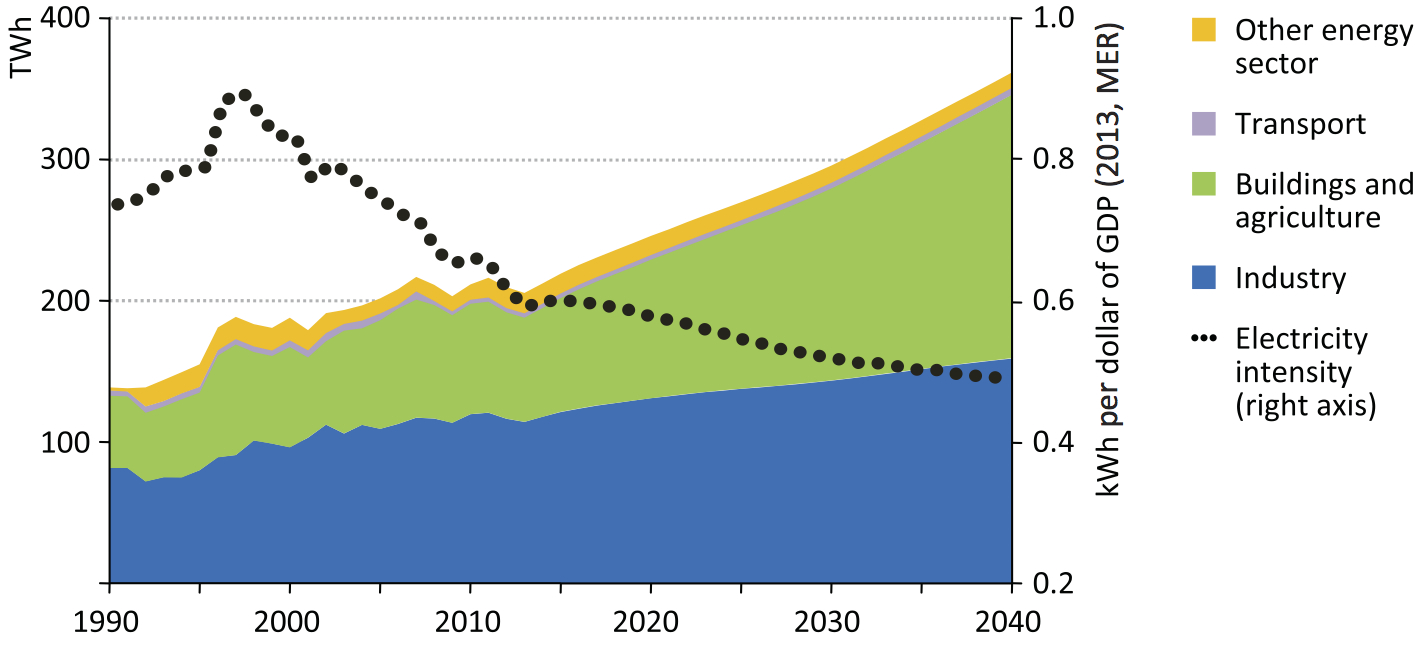
\includegraphics[width=0.9\linewidth]{FIG/SA_Electricity_demand_growth}
\caption[Electricity demand growth by sector in South Africa in the New Policies Scenario.]{Electricity demand growth by sector in South Africa in the New Policies Scenario \cite{IEA2014f}.}\label{Abb1}
\end{figure}

\subsection{Structure of power distribution}
Kilometerlängen, Verluste im Netz \cite{Eskom2014a}

On mainland sub-Saharan Africa, SA has with around 85~\% the highest electrification rate. About 11~\% of households don't have access to electricity and a further 4~\% rely on illegal access (non-paying) or obtain access informally (from one household to another but paying). \cite{IEA2014f}

\begin{figure}[htbp] % Netzstrucktur
\centering
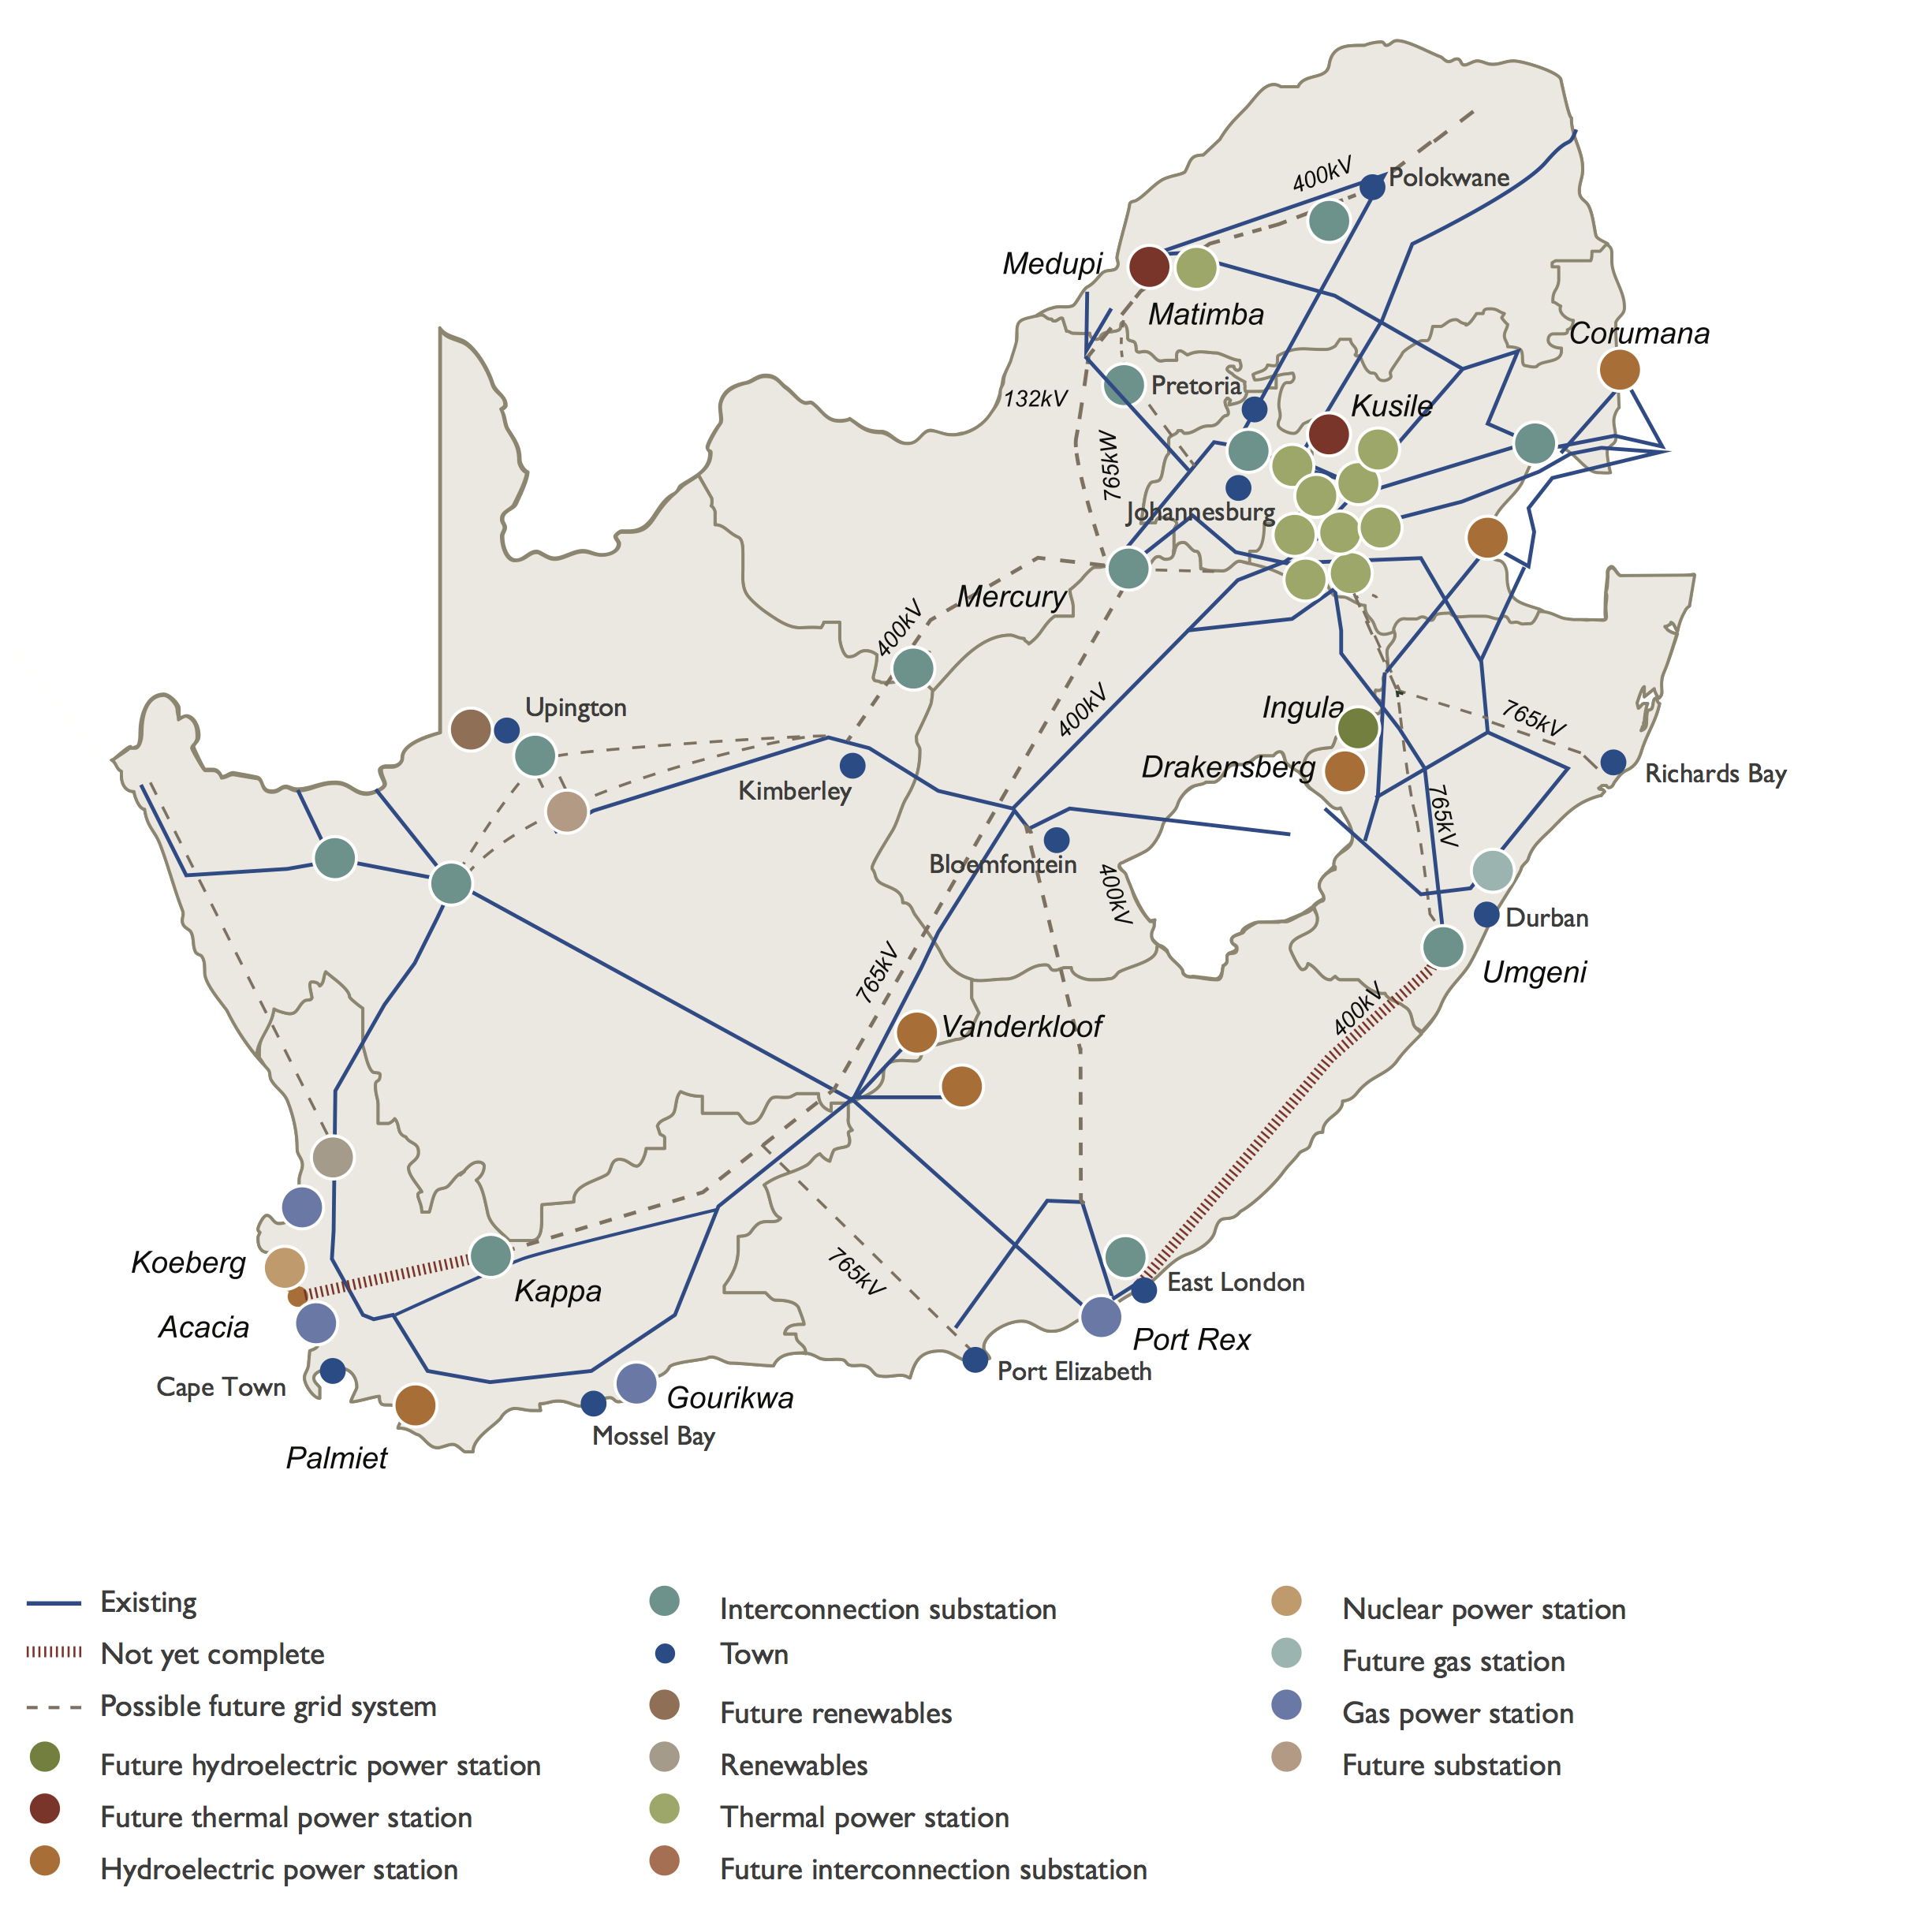
\includegraphics[width=0.9\linewidth]{FIG/transmissionprojekts}
\caption[Eskom’s transmission projects as at 31 March 2014.]{Eskom’s transmission projects as at 31 March 2014 \cite{Eskom2014}.}\label{Abb1}
\end{figure}

http://integratedreport.eskom.co.za/supplementary/app-transmission.php

\section{Renewable energy potential in South Africa}

\subsection{Energy outlook for South Africa}
Development of a Renewable Energy Power Supply Outlook 2015 for the Republic of South Africa
Achieved by Sebastian Giglmayr, BSc
\cite{Giglmayr2013}

\subsection{Government Incentives}

\section{Chapter summary}
\pagebreak

\chapter{Solar energy and system load in South Africa}\label{Solar power in South Africa}
%Almost all power that we use on our planet comes from the sun. Direct in form of radiation or indirect during wind, water and vegetation. Also the fossil power resources and reserves are stored energy from the sun in from of organic carbon compounds.

%The sun emits a power rate of about 3.83x10\textsuperscript{26}W. Of this total, only a tiny fraction, \SI{1367}{\watt\per\square\metre} (solar constant) reaches the Earth’s atmosphere. The solar radiation is reduced by absorption and reflection effects in the atmosphere.  The reduction is about \SI{30}{\percent} on a clear day and about \SI{90}{\percent} on a very cloudy day. \cite{Stine2001a}

The sun's radiative power is \SI{3.83e26}{\watt}, only a tiny fraction of which, \SI{1367}{\watt\per\square\metre} (the solar constant), reaches the Earth’s atmosphere. The solar radiation is reduced by absorption and reflection effects in the atmosphere.  The reduction is about approximately \SI{30}{\percent} on a clear day and approximately \SI{90}{\percent} on a very cloudy day \cite{Stine2001a}.

%When taking an eye on the world map in Figure~\ref{WorldDNI} it can be noticed that some parts of the world receive much higher direct parts of the sun’s irradiation than others. In particular four regions worldwide are worth mentioning. The Atacama Desert in South America, the Mojave Desert in North America, a huge part of Australia and parts of the southern Africa. Therefore SA is one of the country with the highest potential for generating solar electricity in the world.
The sun's radiation does not strike the Earth's surface uniformly, meaning that some parts of the world receive much more direct irradiation than others (Figure~\ref{WorldDNI}). South Africa is one of the four regions of the Earth's surface that receive the highest portion of direct normal irradiation, making it an ideal for solar electricity generation.

\begin{figure}[h!] 
\centering
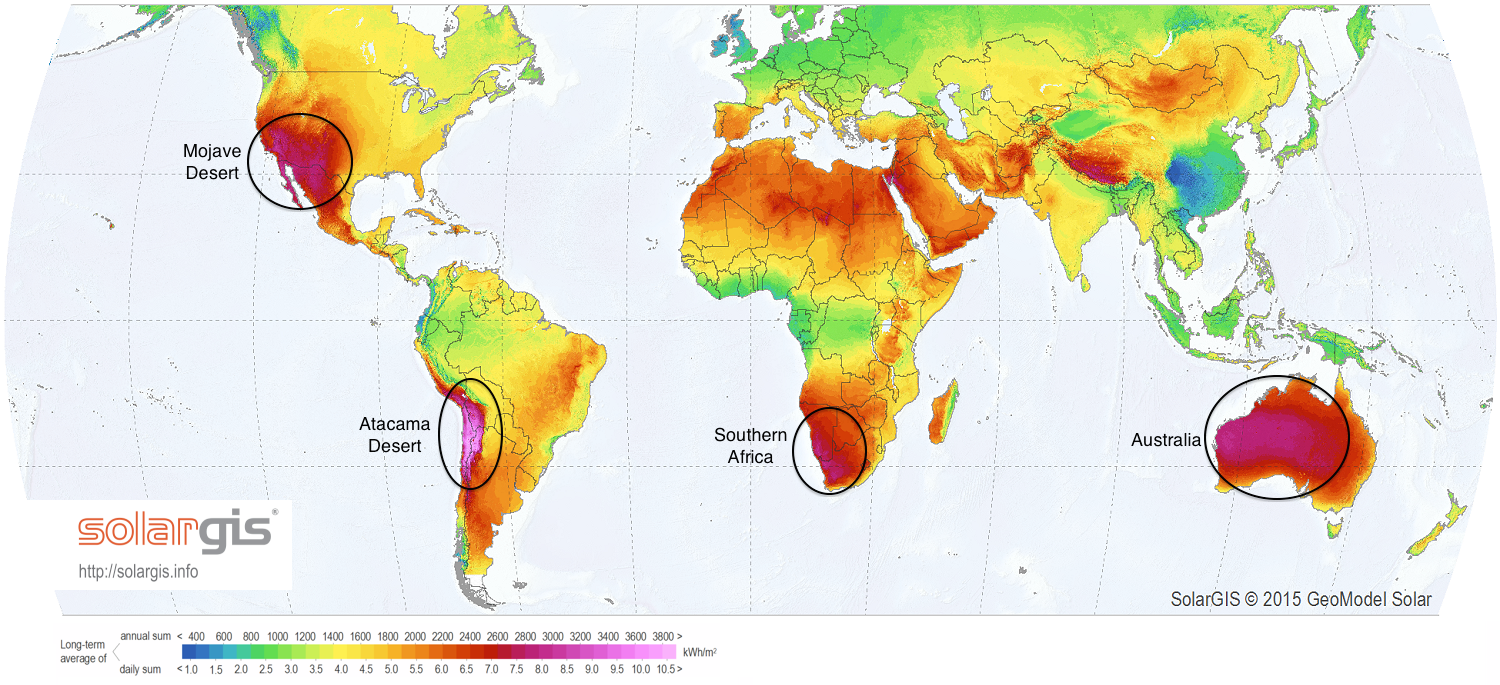
\includegraphics[width=1\linewidth]{FIG/WorldDNI}
\caption[World map of Direct normal irradiation.]{World map of Direct normal irradiation \cite{SolarGIS2015c}.}\label{WorldDNI}
\end{figure}  
\pagebreak
\section{Solar radiation} \label{Solar radiation}
%As shown above, solar irradiation is highly depending from the location. The solar irradiance of a specific location can be measured on-site by ground measurement devices or site-adapted by interpolated satellite data, which is validated with other ground measurement devices \cite{Paulescu2013}. Thereby is the direct and indirect as well as the total sun irradiance crucial.
Solar irradiation can be highly variable, depending on the location, so accurate on-site measurement and differentiation of direct and indirect irradiance are crucial. The solar irradiance of a specific location can be measured on-site by ground measurement devices or site-adapted by interpolated satellite data, which is validated with other ground measurement devices \cite{Paulescu2013}.

%These solar irradiation parameter are here defined:
Solar irradiation parameters are defined here.

\begin{itemize}
\item \textbf{\emph{Global Horizontal Irradiance} (GHI)} in \si{\kilo\watt\hour\per\square\metre\per\year} or \si{\watt\per\square\metre}: GHI is the total amount of shortwave radiation received from above by a horizontal surface. It includes direct (beam) and a diffuse (scattered) irradiation. This value is of particular interest when designing PV or solar water heater systems with a fixed inclined angle.
\item \textbf{\emph{Direct Normal Irradiance} (DNI)} in \si{\kilo\watt\hour\per\square\metre\per\year} or \si{\watt\per\square\metre}: DNI is the amount of solar radiation received per unit area by a surface that is always held perpendicular (or normal) to the rays that come in a straight line from the direction of the sun at its current position in the sky. Diffuse irradiation is totally excluded from the DNI. This quantity is relevant for installations that track the position of the sun.
\item \textbf{\emph{Diffuse Horizontal Irradiance} (DHI)} in \si{\kilo\watt\hour\per\square\metre\per\year} or \si{\watt\per\square\metre}: DHI is the amount of radiation received per unit area by a surface that does not arrive on a direct path from the sun, but has been scattered by molecules and particles in the atmosphere and comes equally from all directions.
\end{itemize}
%Furthermore is irradiance understood as instantaneous density of solar radiation incident on a given surface, typically expressed in W/m\textsuperscript{2} and irradiation is the sum of irradiance over a time period expressed in J/m\textsuperscript{2} or more commonly used in Wh/m\textsuperscript{2}. The connection between the solar radiation parameters is shown in Equation \ref{GL_GHI}.The angle $\theta_\text{z}$ is the angle between the direction of the sun and the zenith (directly overhead).
\emph{Irradiance} is understood as the instantaneous density of solar radiation incident on a given surface and is typically expressed in \si{\watt\per\square\metre} and \emph{irradiation} is the sum of irradiance over a time period expressed in \si{\joule\per\square\metre} or the more commonly used \si{\watt\hour\per\square\metre}. The relationship between solar radiation parameters is shown by Equation \ref{GL_GHI}.The angle $\theta_\text{z}$ is the angle between the direction of the sun and the zenith (directly overhead).
\begin{align}
\text{GHI}=\text{DNI}\cdot\cos(\theta_{z})+\text{DHI}\label{GL_GHI}
\end{align}

The GHI is a determining factor for the power output of PV systems and the DNI for CSP systems. In South Africa, the ceiling for GHI is more than \SI{2300}{\kilo\watt\hour\per\square\metre\per\year}, while in some parts of the country DNI is as high as \SI{2900}{\kilo\watt\hour\per\square\metre\per\year} (Figure\ref{irradiation}), significantly higher than in most regions of the world. The highest GHI occurs close to the Namibian border in the northwest. The direct beam is also at its highest in western SA. The area around Springbok in Northern Cape province has the highest DNI.

\begin{figure}[h!]
        \centering
        \begin{subfigure}[b]{0.5\textwidth}
                \centering
                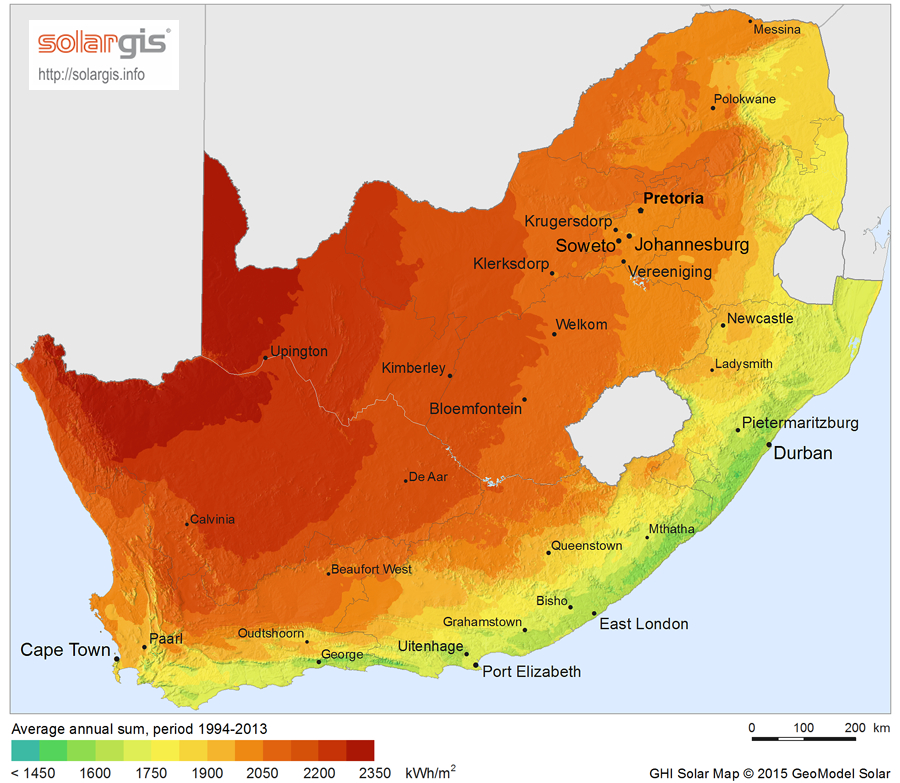
\includegraphics[width=1\textwidth]{FIG/SA_GHI}
                \caption{Global Horizontal Irradiation \cite{SolarGIS2015a}.}\label{fig:bild-links}
        \end{subfigure}%
        ~
        \begin{subfigure}[b]{0.5\textwidth}
                \centering
                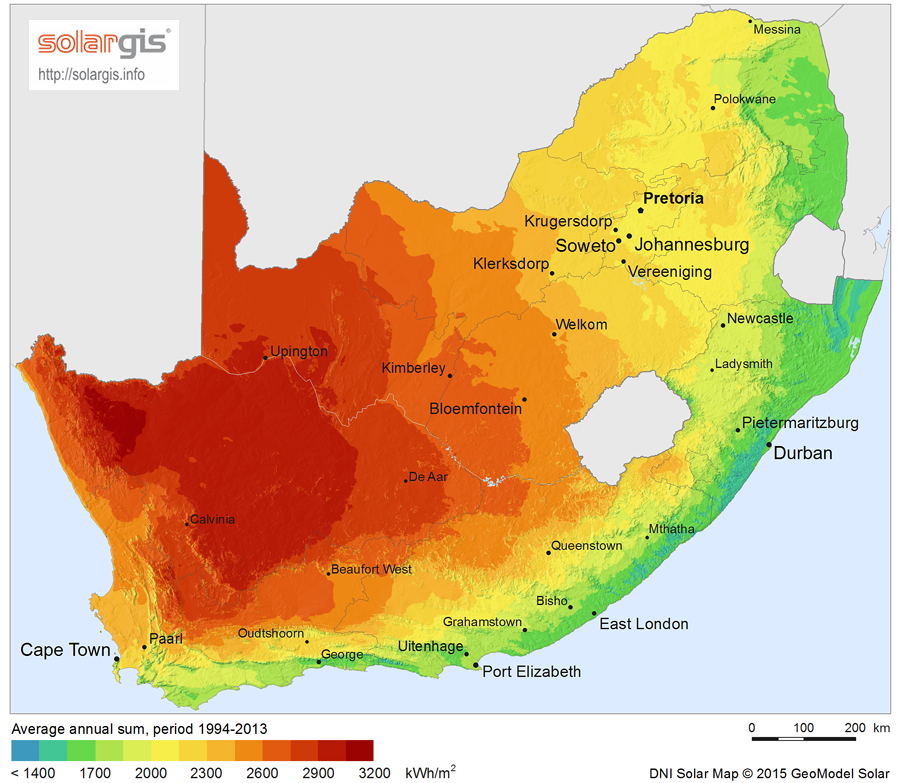
\includegraphics[width=1\textwidth]{FIG/SA_DNI}
                \caption{Direct Normal Irradiation \cite{SolarGIS2015b}.}\label{fig:bild-rechts}
        \end{subfigure}
        \caption{Solar radiation maps of South Africa.}\label{irradiation}
\end{figure}
\pagebreak
%Both maps demonstrates, that the highest values of solar irradiation can be found in the northwestern part of SA, which allocated in the Northern Cape Province. Currently all CSP plants and about two-thirds of the PV systems of SA are developed in the Northern Cape \cite{Forder2015}. Thereby the region around the city of Upington is highly attractive, owning to the high irradiation value in connection with a reliable water access due to the Orange River and the possibility of a close access to the Eskom grid. 

Currently all CSP plants and about two-thirds of the PV systems in South Africa are located in the Northern Cape \cite{Forder2015}. The region around the city of Upington is particularly attractive, owing to the high irradiation value and reliable water access through the Orange River and proximity to the Eskom grid.

%Therefore the location parameter and weather data of Upington was selected for the simulation and calculations in this thesis \cite{WhiteBoxTechnologies2015}. The hourly values of GHI and DNI over a full year for Upington are shown in Figure~\ref{Upington_GHI/DNI}. The highest irradiance value during the summer are \SI{1199}{\watt\hour\per\square\metre} for GHI and \SI{1154}{\watt\hour\per\square\metre} for DNI. At the northern solstice, the highest irradiance is \SI{625}{\watt\hour\per\square\metre} for GHI and \SI{820}{\watt\hour\per\square\metre} for DNI. 
The environmental parameters and weather data for Upington were selected for the simulation and calculations performed for this work \cite{WhiteBoxTechnologies2015}. The hourly values of GHI and DNI over a full year are shown for Upington (Figure~\ref{Upington_GHI/DNI}). The highest irradiance values during the summer are \SI{1199}{\watt\hour\per\square\metre} GHI and \SI{1154}{\watt\hour\per\square\metre} DNI. At the northern solstice, the highest irradiance is \SI{625}{\watt\hour\per\square\metre} GHI and \SI{820}{\watt\hour\per\square\metre} DNI. 

%Irradiation values demonstrate significant seasonal variation of GHI with high values in summer and low irradiation in winter, whereas the DNI shows a more balanced variation throughout the year. This mainly leads from the irradiation angle which is changing constantly during the year. 
Irradiation values demonstrate significant seasonal variation in GHI in comparison to DNI, with high values in summer and low irradiation in winter. This is the result of the irradiation angle, which changes constantly throughout the year. 


\begin{figure}[!htbp]
        \centering
                \begin{subfigure}[b]{1\textwidth}
                \centering
                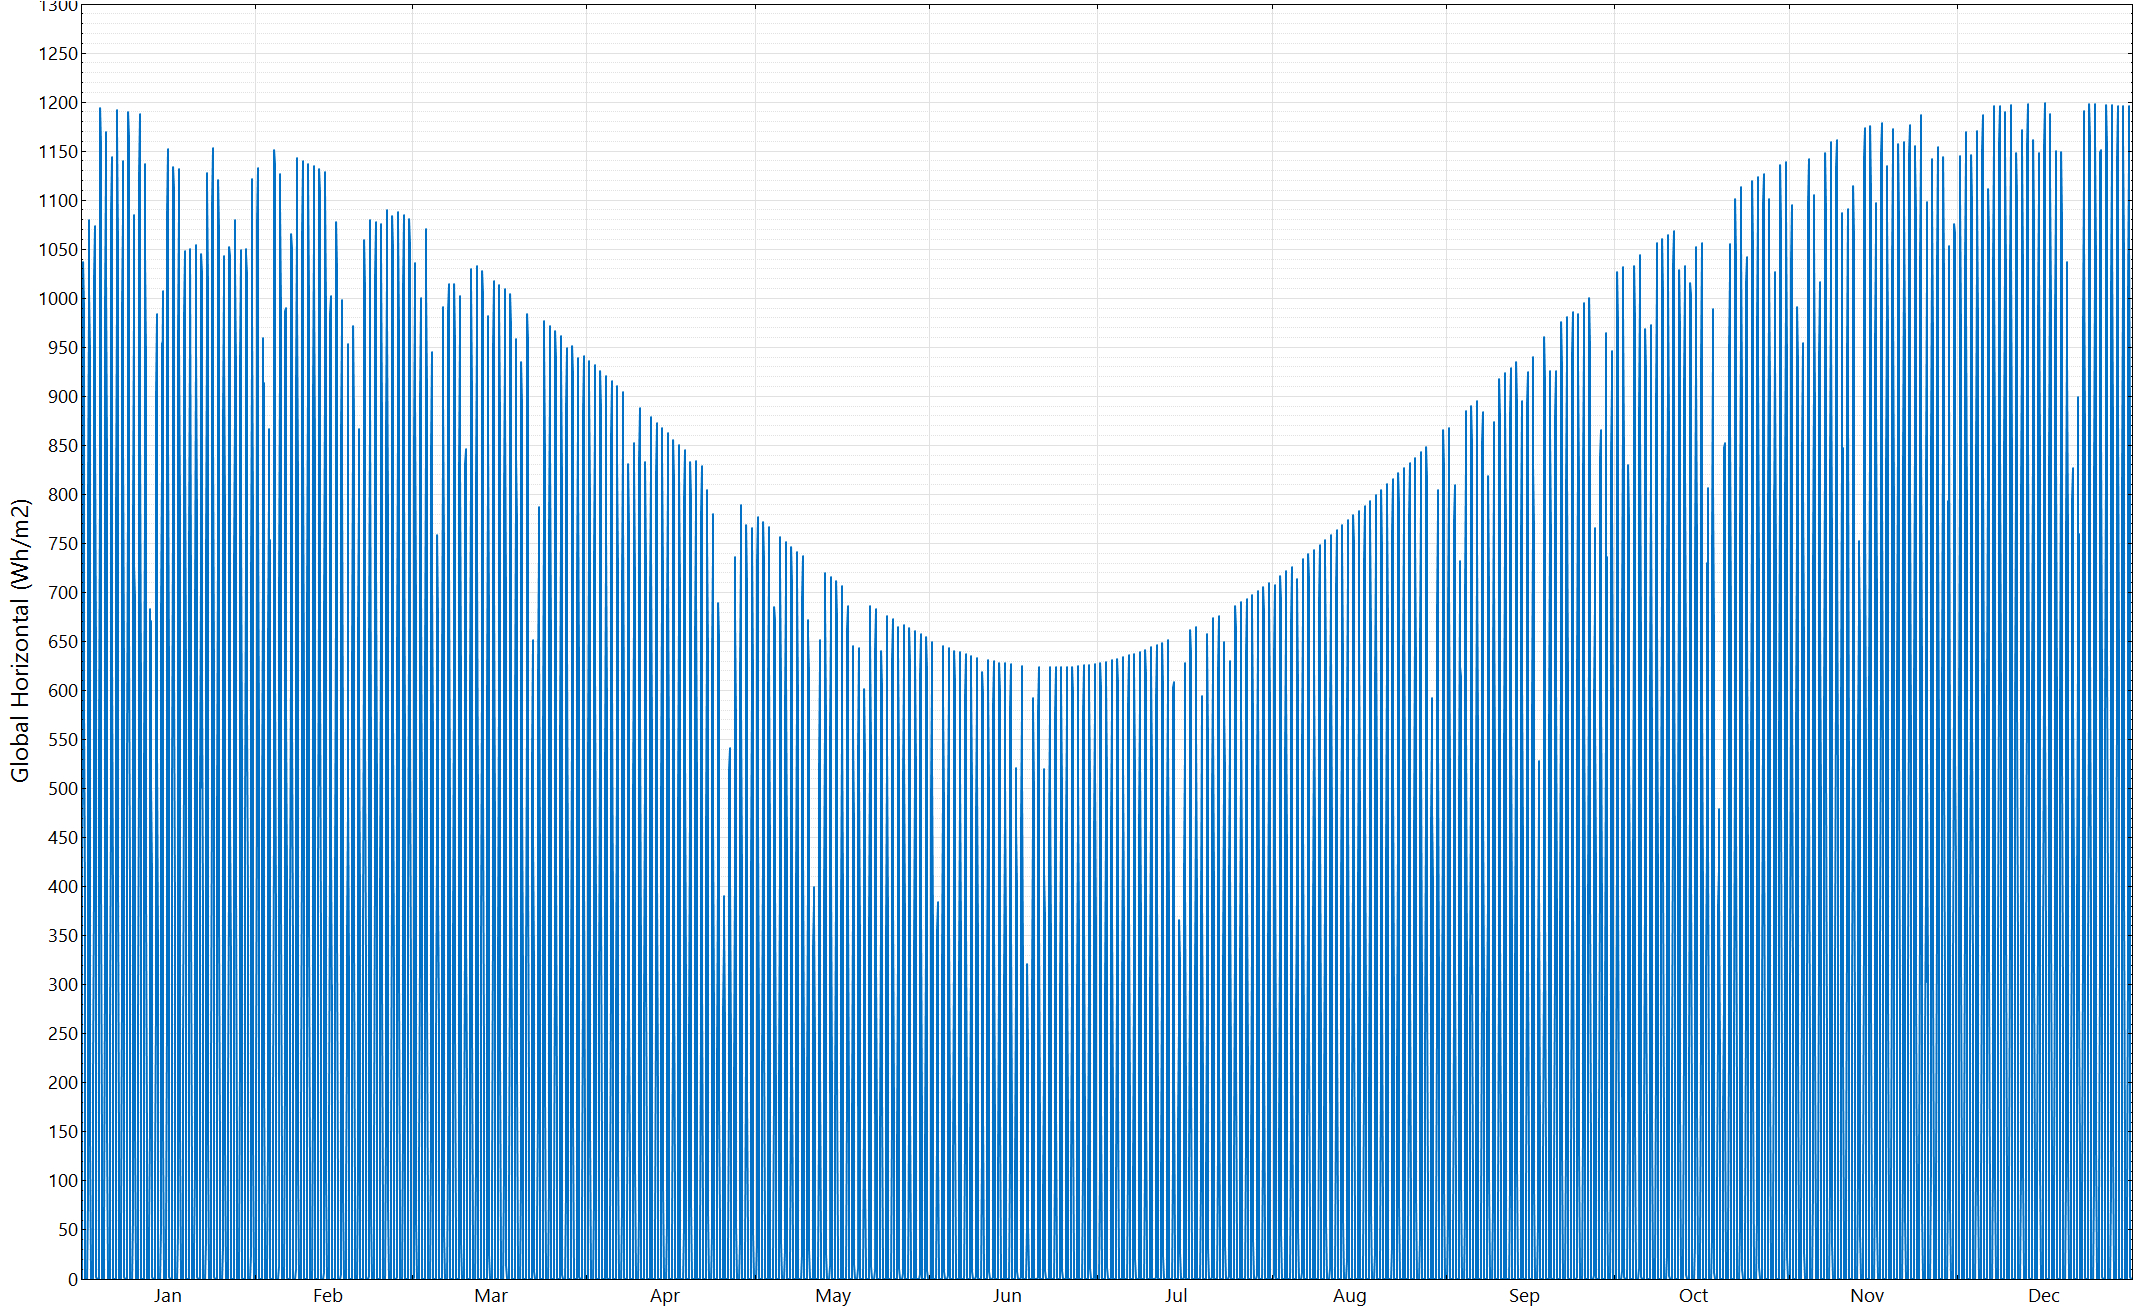
\includegraphics[width=1\textwidth]{FIG/Upington_GHI}
                \caption{Global horizontal irradiance}\label{Upington_GHI}
        \end{subfigure}
\par\medskip % Linebreak      
        \begin{subfigure}[b]{1\textwidth}
                \centering
                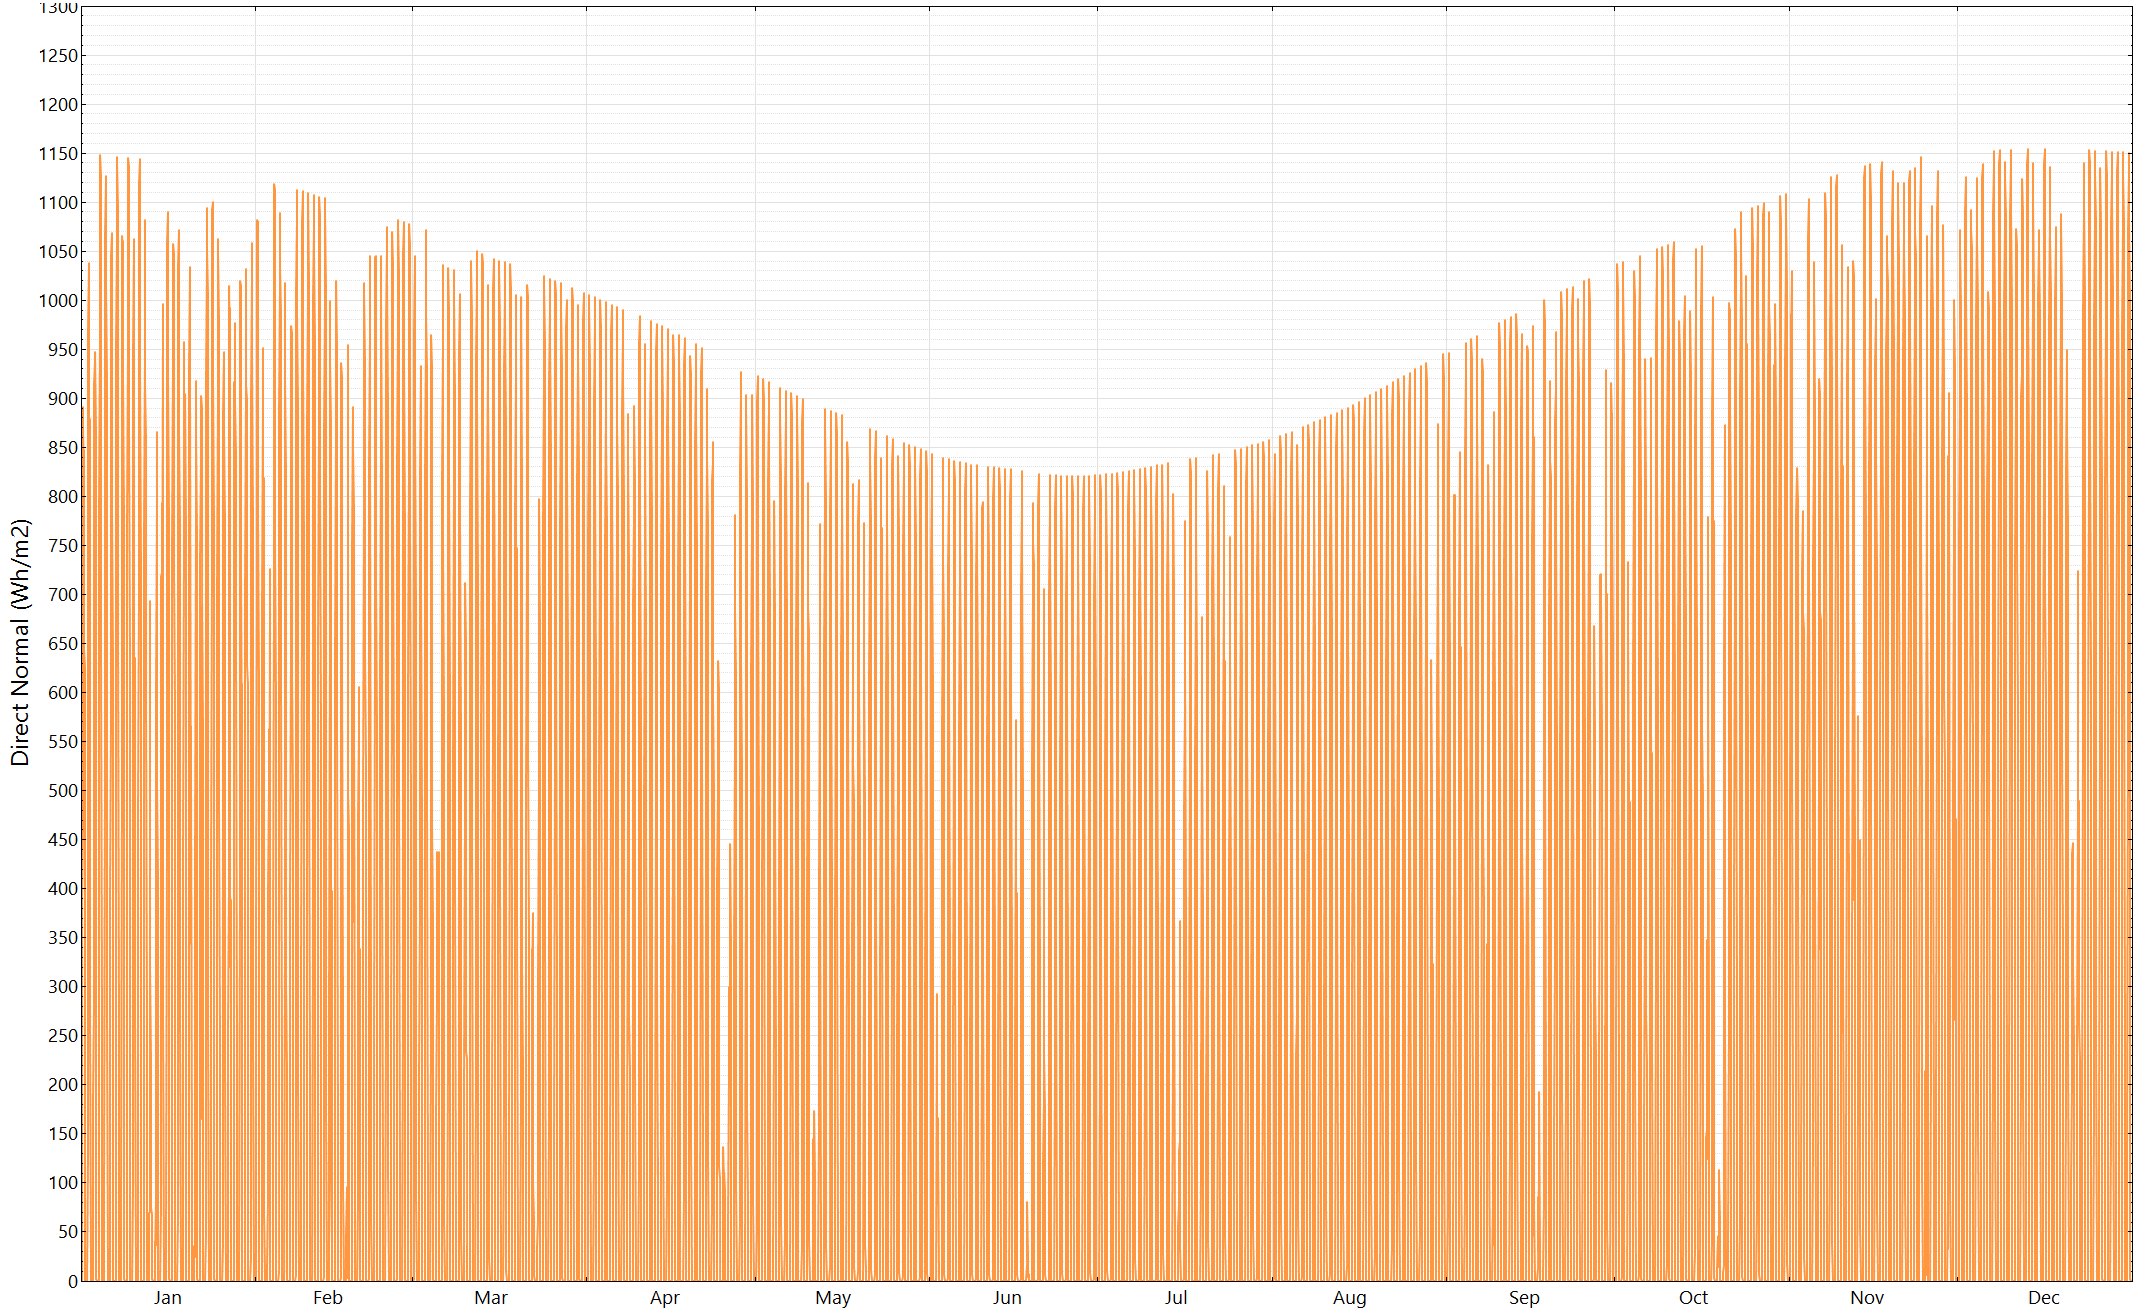
\includegraphics[width=1\textwidth]{FIG/Upington_DNI}
                \caption{Direct normal irradiance}\label{Upington_DNI}
        \end{subfigure}

        \caption[Hourly values of irradiance over a full year from Upington used for the simulation.]{Hourly values of irradiance over a full year from Upington used for the simulation.}\label{Upington_GHI/DNI}
\end{figure}
%The path of the sun during the year in Upington is characterize in Figure~\ref{SunPathUpington}. The solar path diagram depends on the geographical location by the position of longitude and latitude. The diagram apparent that the longest day in Upington has a duration of \SI{13}{h} and \SI{56}{minutes} with a maximum sun height of \SI{85.05}{\degree} while the shortest day has a duration of just \SI{10}{h} and \SI{19}{minutes} and a maximum sun height of \SI{35.93}{\degree}.
The solar path for Upington is characterized in Figure~\ref{SunPathUpington}. The longest day has a duration of \SI{13}{h} and \SI{56}{minutes} with a maximum sun height of \SI{85.05}{\degree}, while the shortest day has a duration of just \SI{10}{h} and \SI{19}{minutes} and a maximum sun height of \SI{35.93}{\degree}.

\begin{figure}[htbp]  
\centering
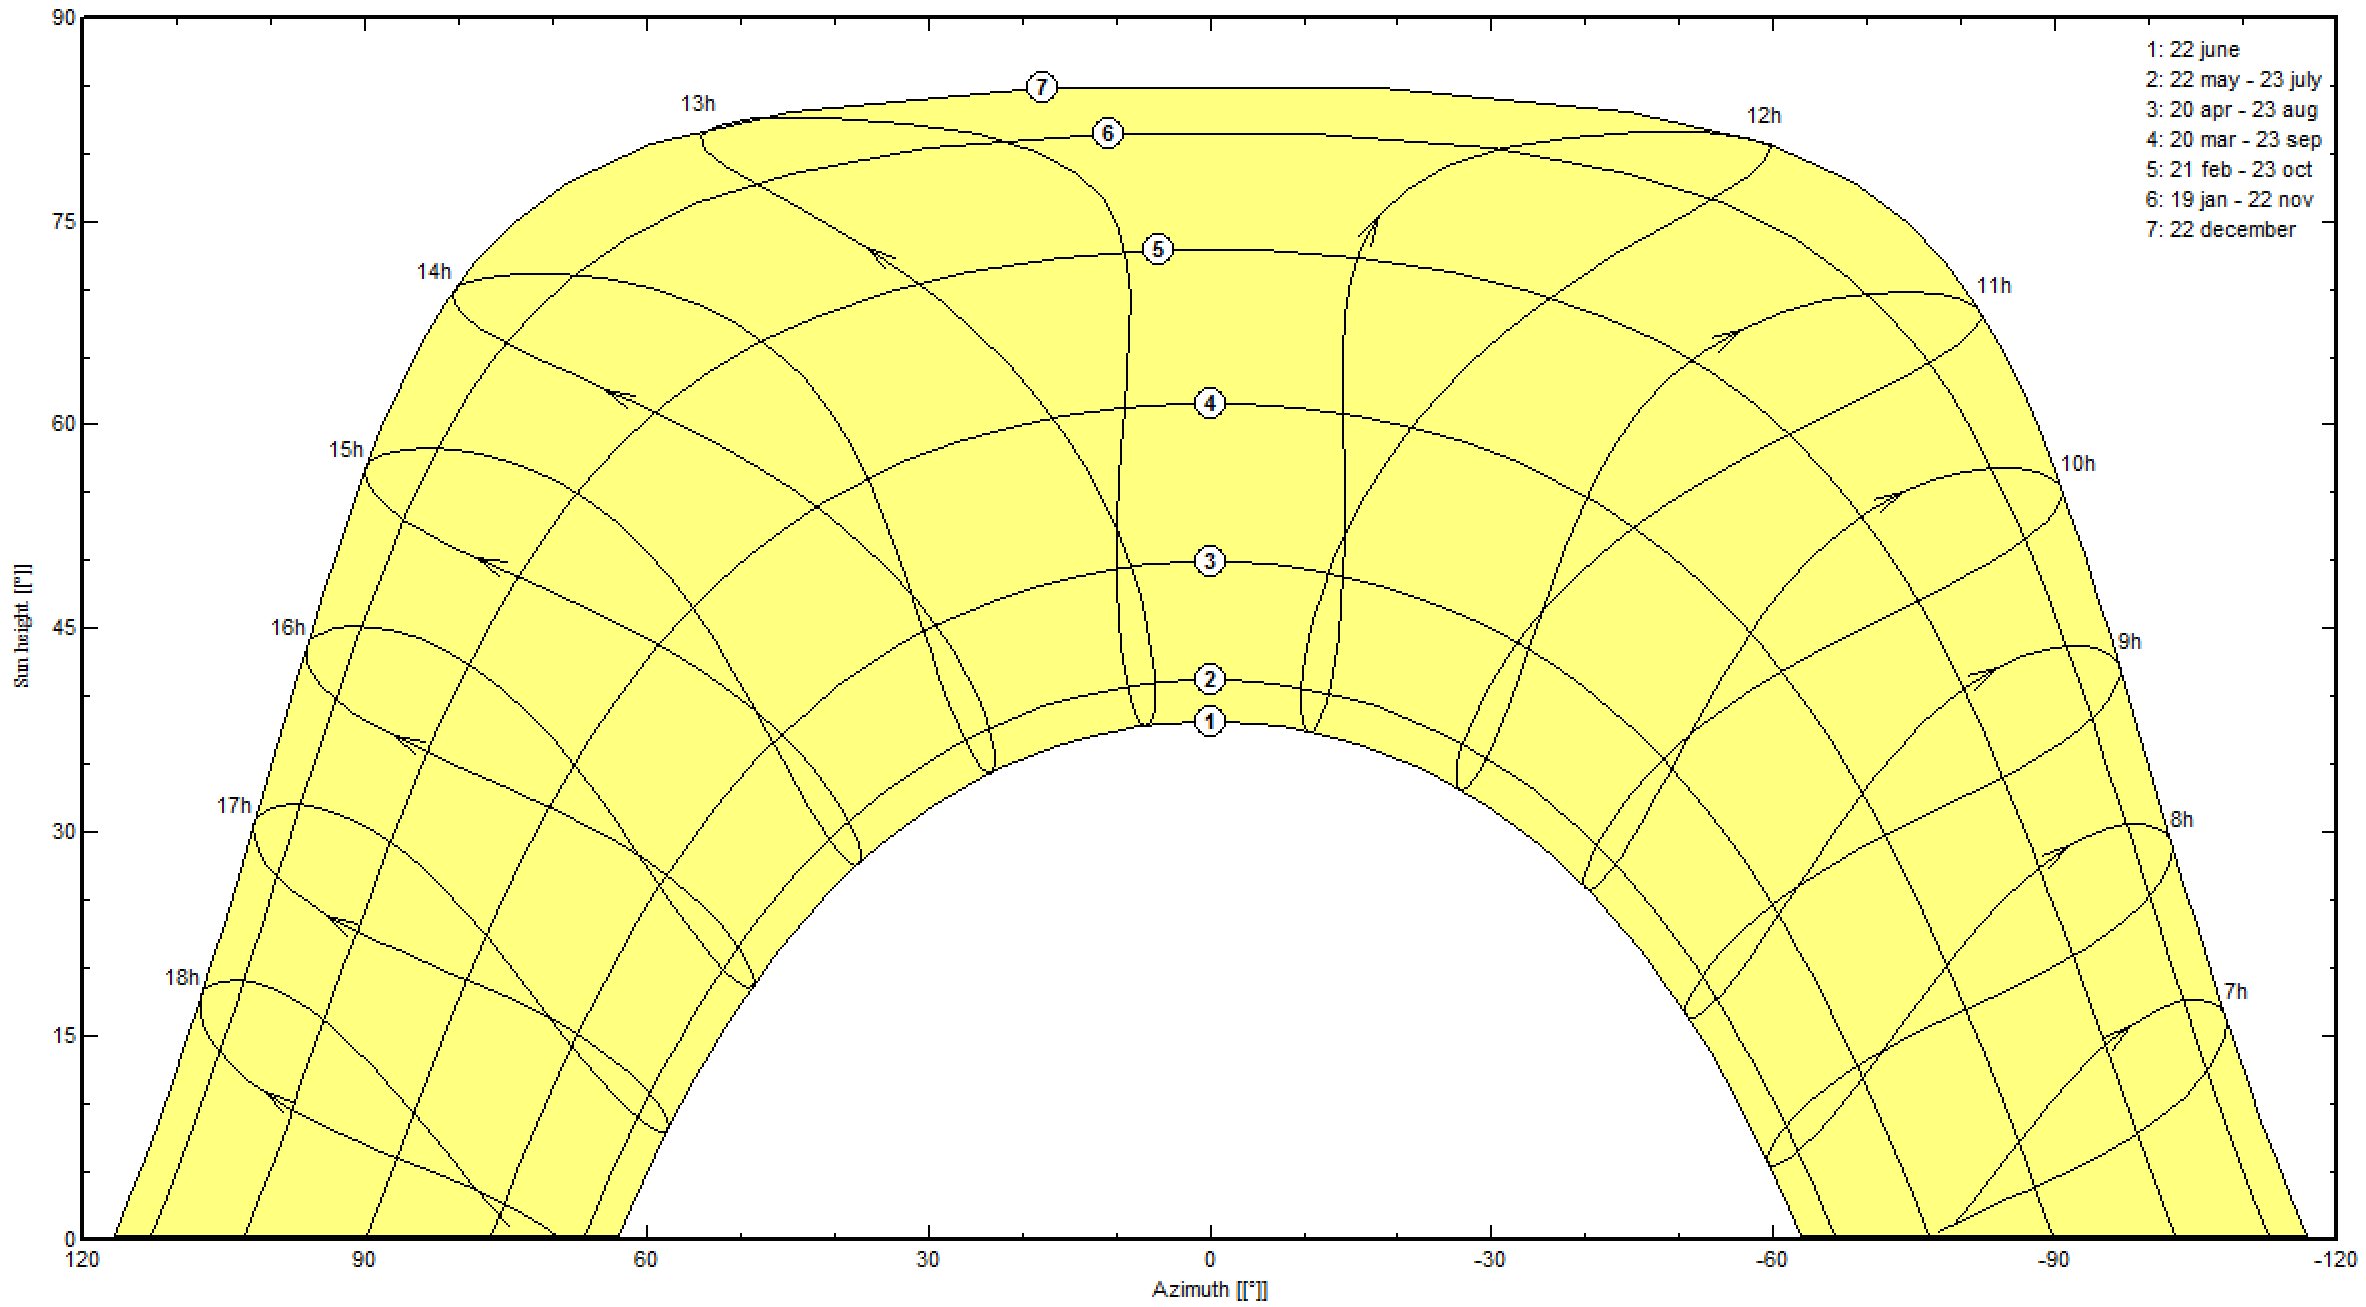
\includegraphics[width=1\linewidth]{FIG/SunPathUpington}
\caption[Solar path diagram for Upington.]{Solar path diagram Upington \cite{PVsystSA2015}.}\label{SunPathUpington}
\end{figure}
\pagebreak
%From the hourly irradiation values concludes a annual sum of \SI{2280}{\kilo\watt\hour\per\square\metre\year} by GHI and an annuall DNI amount of \SI{2621}{\kilo\watt\hour\per\square\metre\year}. When comparing this for the simulation used data with the solar irradiation maps in Figure~\ref{irradiation} the annual sum of GHI is corresponding. But it must be noted that the annual sum of DNI from SolarGIS map \cite{SolarGIS2015b} is about \SI{200}{\kilo\watt\hour\per\square\metre\year} higher than the value which was used for the simulation in this thesis.

The annual totals are \SI{2280}{\kilo\watt\hour\per\square\metre\year} via GHI and \SI{2621}{\kilo\watt\hour\per\square\metre\year} via DNI. When comparing the data used for the simulation with the solar irradiation maps in Figure~\ref{irradiation}, note that the annual total DNI acccording to SolarGIS \cite{SolarGIS2015b} is about \SI{200}{\kilo\watt\hour\per\square\metre\year} higher than the value used for the simulation in this thesis.

The weather data for the simulation are in EPW format (EnergyPlus Weather Data) and produced by White Box Technologies, Inc. \cite{WhiteBoxTechnologies2015}. The EPW files are data sets of hourly values of solar radiation and meteorological elements for a typical one-year period. These include air temperature (\si{\celsius}), dew point temperature (\si{\celsius}), relative humidity (\si{\percent}), atmospheric pressure(\si{\milli\bar}), global horizontal solar radiation (\si{\watt\per\square\metre}), diffuse horizontal solar radiation (\si{\watt\per\square\metre}), direct normal radiation (\si{\watt\per\square\metre}), wind speed (\si{\metre\per\second}), wind direction (\si{\degree}) and snow depth (\si{\metre}). The most relevant parameters for the simulation are summarized in Table \ref{tbl: Location}. 
 
\begin{table}[!h]  
  \centering
	\begin{tabular}{  p{4.0cm}  C{4.0cm}  C{3.0cm} } 
	\hline	
\textbf{Item}  & \textbf{Value} & \textbf{Unit} \\ \hline \hline
Location & Upington & -\\ 
Station ID &  684240& -  \\ 
Data source & White Box Technologies, Inc. (31.05.2015) & -\\ \hline
Latitude & -28.40 &$\,^{\circ}$N \\ 
Longitude &  21.27 &$\,^{\circ}$E \\ 
Elevation &  836 & m \\ 
Total GHI per year  &  2~280 & \si{\kilo\watt\hour\per\square\metre}\\ 
Total DNI per year &  2~621 & \si{\kilo\watt\hour\per\square\metre}\\ 
Total DHI per year &  516 & \si{\kilo\watt\hour\per\square\metre}\\ 
Mean temp. &  21 & \si{\celsius}\\ 
Mean wind speed & 3.3 & \si{\metre\per\second}\\ \hline
\end{tabular}
\caption[Location and characteristics for the simulation in SAM.]{Location and characteristics for the simulation in SAM.}\label{tbl: Location}
\end{table}
\pagebreak

\section{Current state of solar electricity generation in South Africa}
South Africa's solar power expansion began with the first round of the Renewable Energy Independent Power Producer Procurement Program (REIPPPP) in 2011, and continues through to the fourth round of the REIPPPP in 2015 (for a breakdown, see Section~\ref{ElectricitySA}). Eskom operates an additional \SI{100}{\mega\watt} CSP project which is not a part of the REIPPPP.

%South Africa started there expansion in the field of solar power plants with the first round of the REIPPPP in 2011. As it was mentioned before in Section~\ref{ElectricitySA} the REIPPPP has currently a capacity of \SI{5237}{\mega\watt} committed inclusive \SI{1899}{\mega\watt} PV systems and \SI{600}{\mega\watt} CSP plants. Additionally comes one CSP project with \SI{100}{\mega\watt} from Eskom which is not a part of the REIPPPP.

%Figure \ref{Solar-map} shows the allocation of all currently committed solar power plants of the REIPPPP. Yellow marked are PV-power plants and CSP plants are marked in orange (some marks cover them mutually). The numbers in the single marks expose in which REIPPPP-Round it belongs.
Figure \ref{Solar-map} shows the location of all REIPPPP solar power plants. Photovoltaic plants are marked in yellow and CSP plants are marked in orange. The numbers in the marks correspond to the applicable REIPPPP round.

%Currently SA has 27 fully operational PV-power plants with a total capacity of \SI{1059.05}{\mega\watt} further six PV-power plants with in total of \SI{442.5}{\mega\watt} are under construction. \cite{Forder2015}

%South Africa has 27 fully operational PV plants with a total capacity of \SI{1059.05}{\mega\watt}. A further six PV-power plants with a total of \SI{442.5}{\mega\watt} are under construction \cite{Forder2015}.
%
%Most of the South African PV-power plants are allocated in the Northern Cape. So 29 out of 45 currently committed PV systems are located there. Five more each in the Western Cape and the North-West Province, three each in the provinces Free State and Limpopo, two in Eastern Cape and one more in the Eastern Cape. \cite{Forder2015}

South Africa has 27 fully operational PV plants with a total capacity of \SI{1059.05}{\mega\watt}, a further six with \SI{442.5}{\mega\watt} are under construction, one more with \SI{75}{\mega\watt} waiting to begin construction (approved and financed) and 12 more in approvals, planning and financing with a total capacity of \SI{813}{\mega\watt}. Of the total, 29 of 45 of the operational and planned plants are located in Northern Cape, five in the Western Cape and the North-West Province, three in Limpopo, two in Free State and one in the Eastern Cape. \cite{Forder2015}


\pagebreak

\begin{figure}[h!]
\centering
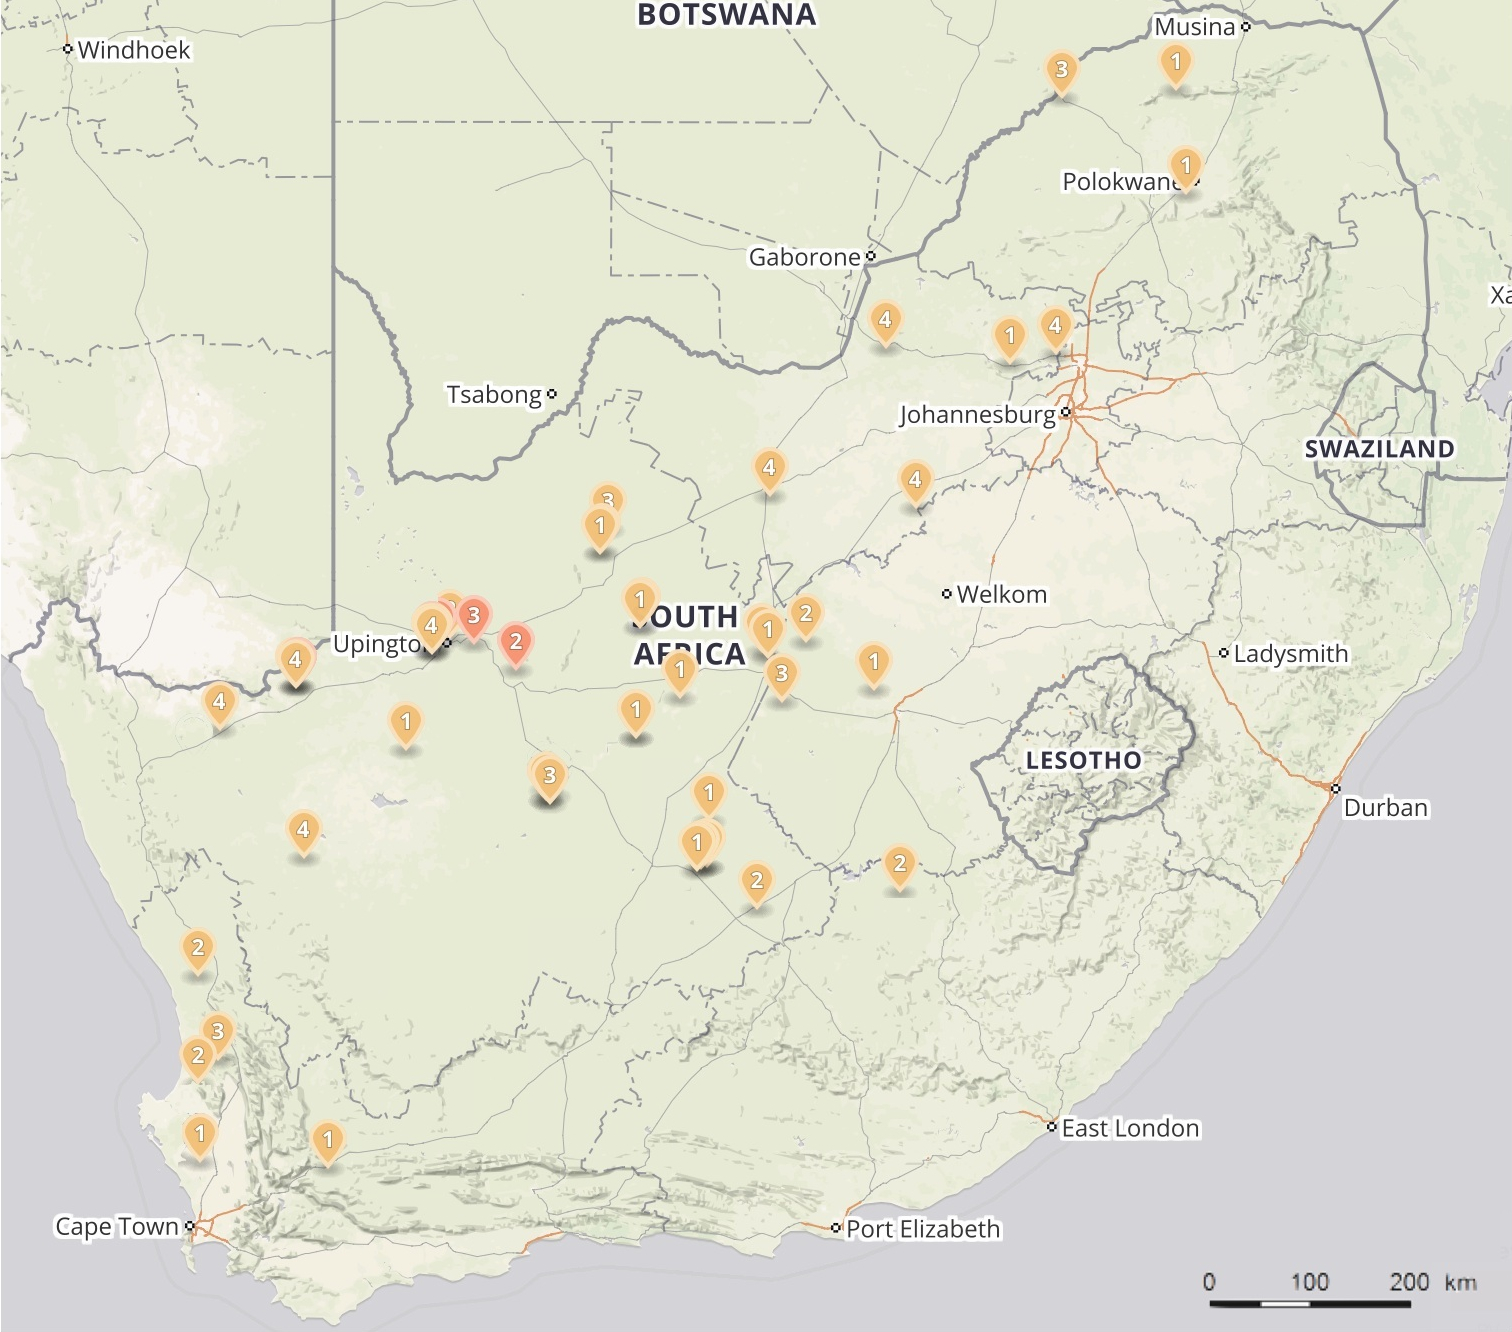
\includegraphics[width=1\linewidth]{FIG/Solar-map}
\caption[Allocation of all REIPPPP solar power plants in SA.]{Allocation of all REIPPPP solar power plants in SA \cite{Forder2015}.}\label{Solar-map}
\end{figure}

%"KaXu Solar One" is the first and currently only full operational CSP plant in SA. It is using parabolic trough technology and a 2.5~h thermal energy storage for generating \SI{100}{\mega\watt} capacity. The CSP-plants "Khi Solar One" and "Bokpoort CSP Project" with a capacity of each 50~MW are under construction as well as the \SI{100}{\mega\watt} "Xina CSP South Africa" project. Further three CSP-plants are awaiting construction, they have all a capacity of each \SI{100}{\mega\watt}. As mentioned before, all eight CSP projects are located in the Northern Cape Province of SA. \cite{Forder2015}

\emph{KaXu Solar One} is the first and so far the only fully operational CSP plant in South Africa. It uses parabolic trough technology with \SI{2.5}{\hour} thermal energy storage for \SI{100}{\mega\watt} generating capacity. The CSP plants \emph{Khi Solar One} and \emph{Bokpoort CSP Project} with a capacity of \SI{50}{\mega\watt} each, as well as the \SI{100}{\mega\watt} projects \emph{Xina CSP South Africa} and \emph{Ilanga CSP 1}, are now under construction. An additional two CSP plants, each with a generating capacity of \SI{100}{\mega\watt} are awaiting construction. \cite{Forder2015}

\pagebreak
\section{System load in South Africa and prescribed load profile} \label{SystemloadinSA}
%The South African supply structure is based on coal-fired thermal power plants, as it was shown in Section~\ref{ElectricitySA} before. But also the renewable energy supply is getting noteworthy for the supply structure in SA. When taking an eye on Figure~\ref{systemload} it can be noted that wind and PV power also makes a small share of the daily electricity supply. It has to be said that by the time of spring in 2014 the KaXu Solar One CSP plant was not completed and so CSP supply in SA doesn't exist. The reveals that the power demand in SA rises in the morning hours and is coming to a peak demand in the evening hours. The surplus energy during the night got compensated by pump storage and reduction by supply imports. 

The South African electricity infrastructure is built on coal-fired thermal power plants, but the renewable energy supply is becoming more important. Wind and PV generation provides a small share of the daily electricity supply (Figure~\ref{systemload})\footnote{By spring 2014, the KaXu Solar One CSP plant was not complete, so CSP is not accounted for in this system load profile.}. Electricity demand rises in the morning hours and peaks at 20:00. The peak demand is covered by pumped storage hydro. 


\begin{figure}[htbp]  
\centering
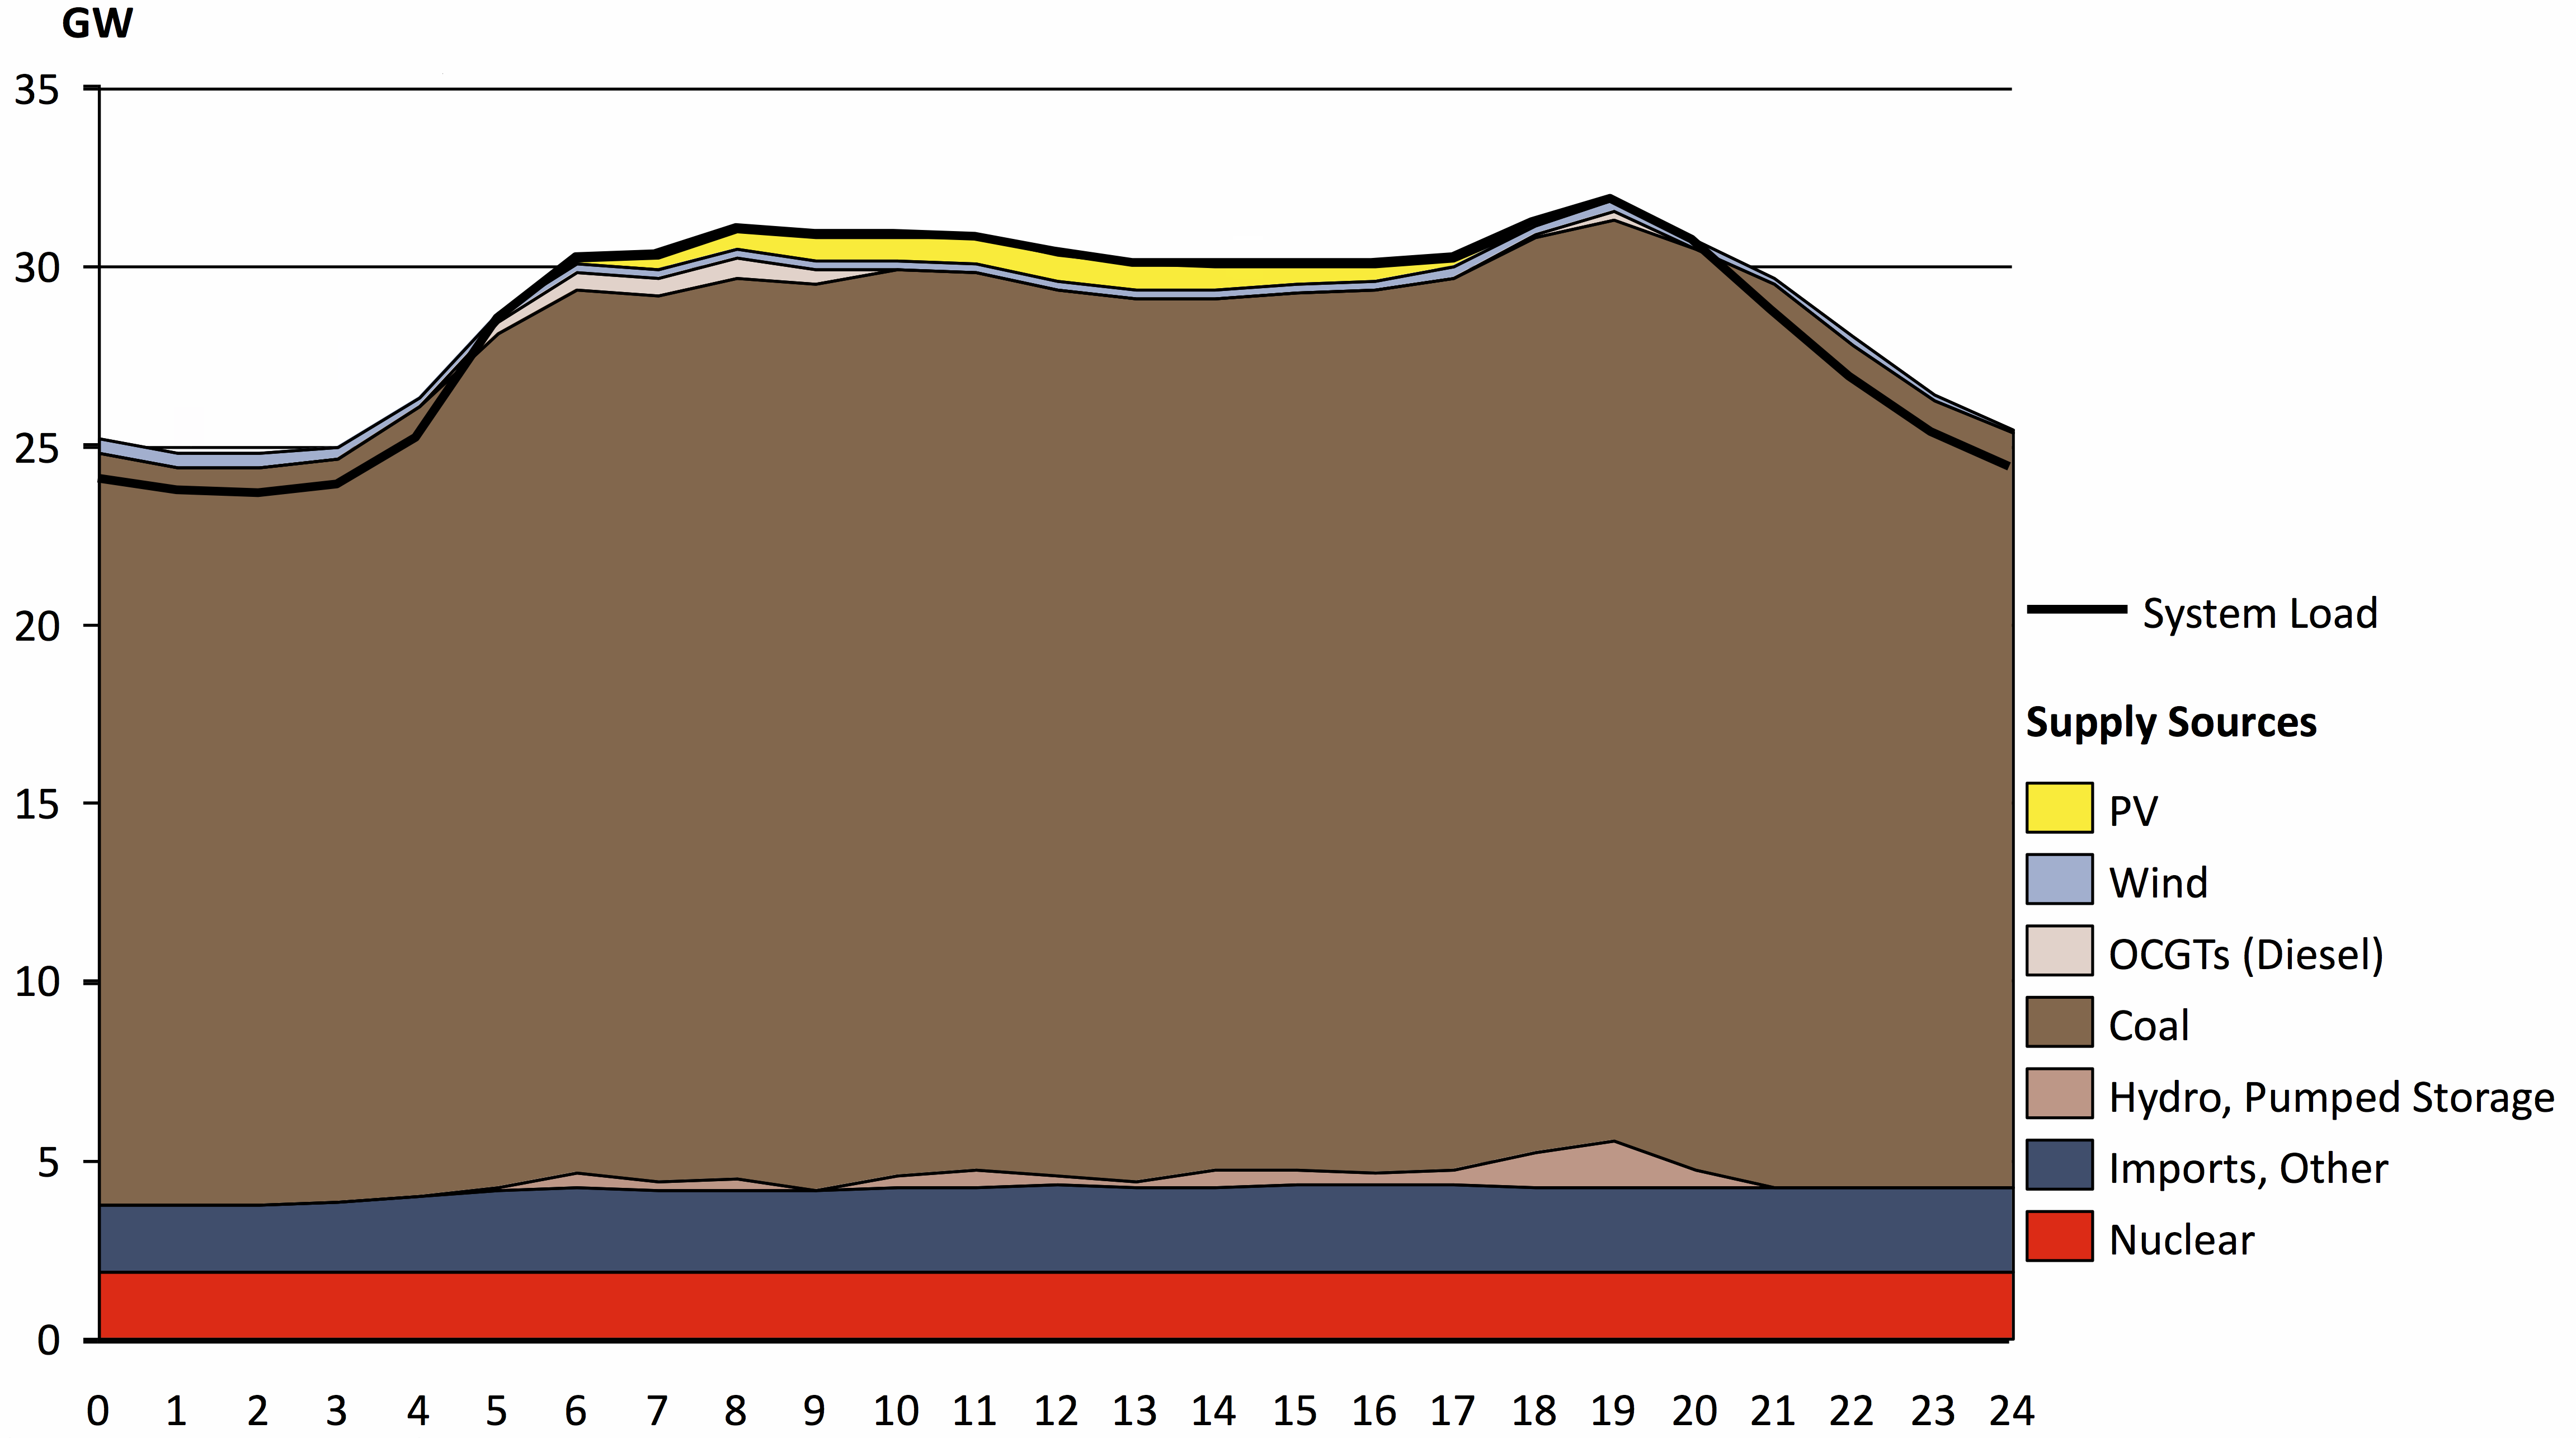
\includegraphics[width=1\linewidth]{FIG/systemload}
\caption[Actual South African supply structure for a spring day, the 17. October 2014.]{Actual South African supply structure for a spring day, the 17. October 2014 \cite{CSIR2015}.}\label{systemload}
\end{figure}
%It is shown that the PV supply can support the South African demand during the day and reduces thereby the generation of coal-fired thermal power plants. But by the time of the daily peak demand, in the evening hours, the PV supply is coming to standstill, whereby this demand needs to be covered by pumped storage or expansive diesel driven open cycle gas turbines (OCGTs).

The PV supply can help meet demand during the day, thereby reducing the need for coal-fired thermal power plants. By the time of the daily peak in the evening hours, however, the PV supply has virtually disappeared. The difference must be covered by pumped storage or expensive diesel-driven open cycle gas turbines (OCGTs).

%When taking an eye on the total unserved energy due to load shedding history of the first half year of 2015 in Figure~\ref{Load_shedding_sum} it is obviously that the capacity bottleneck in SA is mostly during the daytime and particularly during the evening peak hours till 22:00. This makes clear in which time period the support of new power plants is necessary for a secure electricity supply in SA.
%The demand squeeze in When taking an eye on the total unserved energy due to load shedding history of the first half year of 2015 in Figure~\ref{Load_shedding_sum} it is obviously that the capacity bottleneck in SA is mostly during the daytime and particularly during the evening peak hours till 22:00. This makes clear in which time period the support of new power plants is necessary for a secure electricity supply in SA.
% Alles überflüssig. Das hast du bereits gesagt.

%\begin{figure}[htbp]  
%\centering
%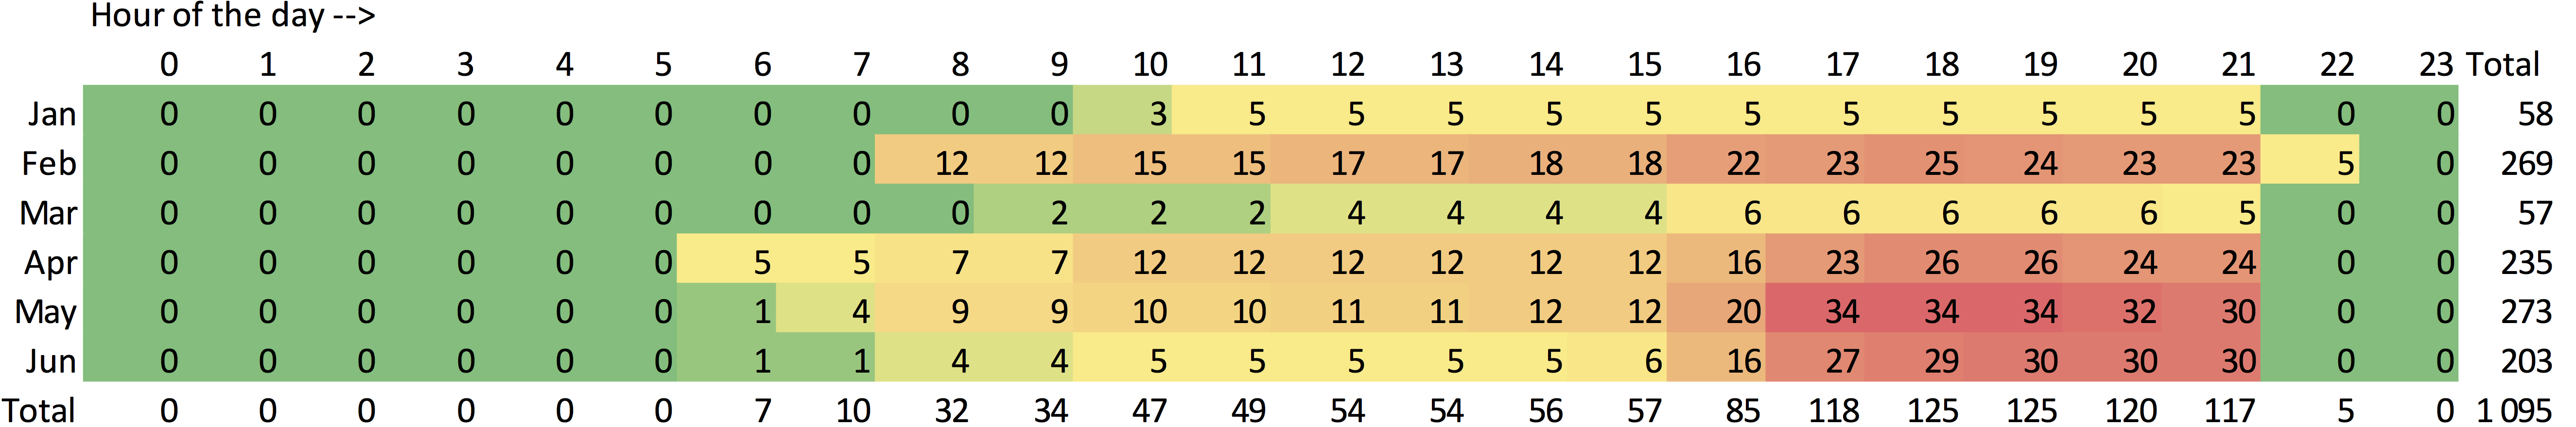
\includegraphics[width=1\linewidth]{FIG/Load_shedding_sum}
%\caption[Total unserved energy due to load shedding for all hours per month Jan-Jun 2015 in GWh.]{Total unserved energy due to load shedding for all hours per month Jan-Jun 2015 in GWh \cite{CSIREnergyCentre2015}.}\label{Load_shedding_sum}
%\end{figure}

%It is a hard requirement that plants meet the full electrical demand in the system. Figure~\ref{LoadScenarios} shows the daily average system load/demand in South Africa for the winter and summer period (2011). It can be seen that the summer profile has a particularly lower demand than the winter profile (up to \SI{15}{\percent} difference) and after a sharp rise at approx 7:00 the demand has a constant system load during the day due to commercial, agricultural and residential demand caused by air-conditioning, pool pumps and geysers, which comes to their peak demand at 20:00. In winter, there is an initial peak at 9:00 and a second at 19:00 mainly caused by residential customers due to electrical heating, lighting, cooking, geysers and pool pumps.

Aggregate demand is lower in summer (Figure~\ref{LoadScenarios}). Summer peaks are flatter and primarily due to commercial, agricultural and residential demand caused by air-conditioning, pool pumps and geysers, peaking at 20:00. Winter peaks at 9:00 and 19:00 are mainly caused by residential customers and are due to electrical heating, lighting, cooking, geysers and pool pumps.

\begin{figure}[htbp]  
\centering
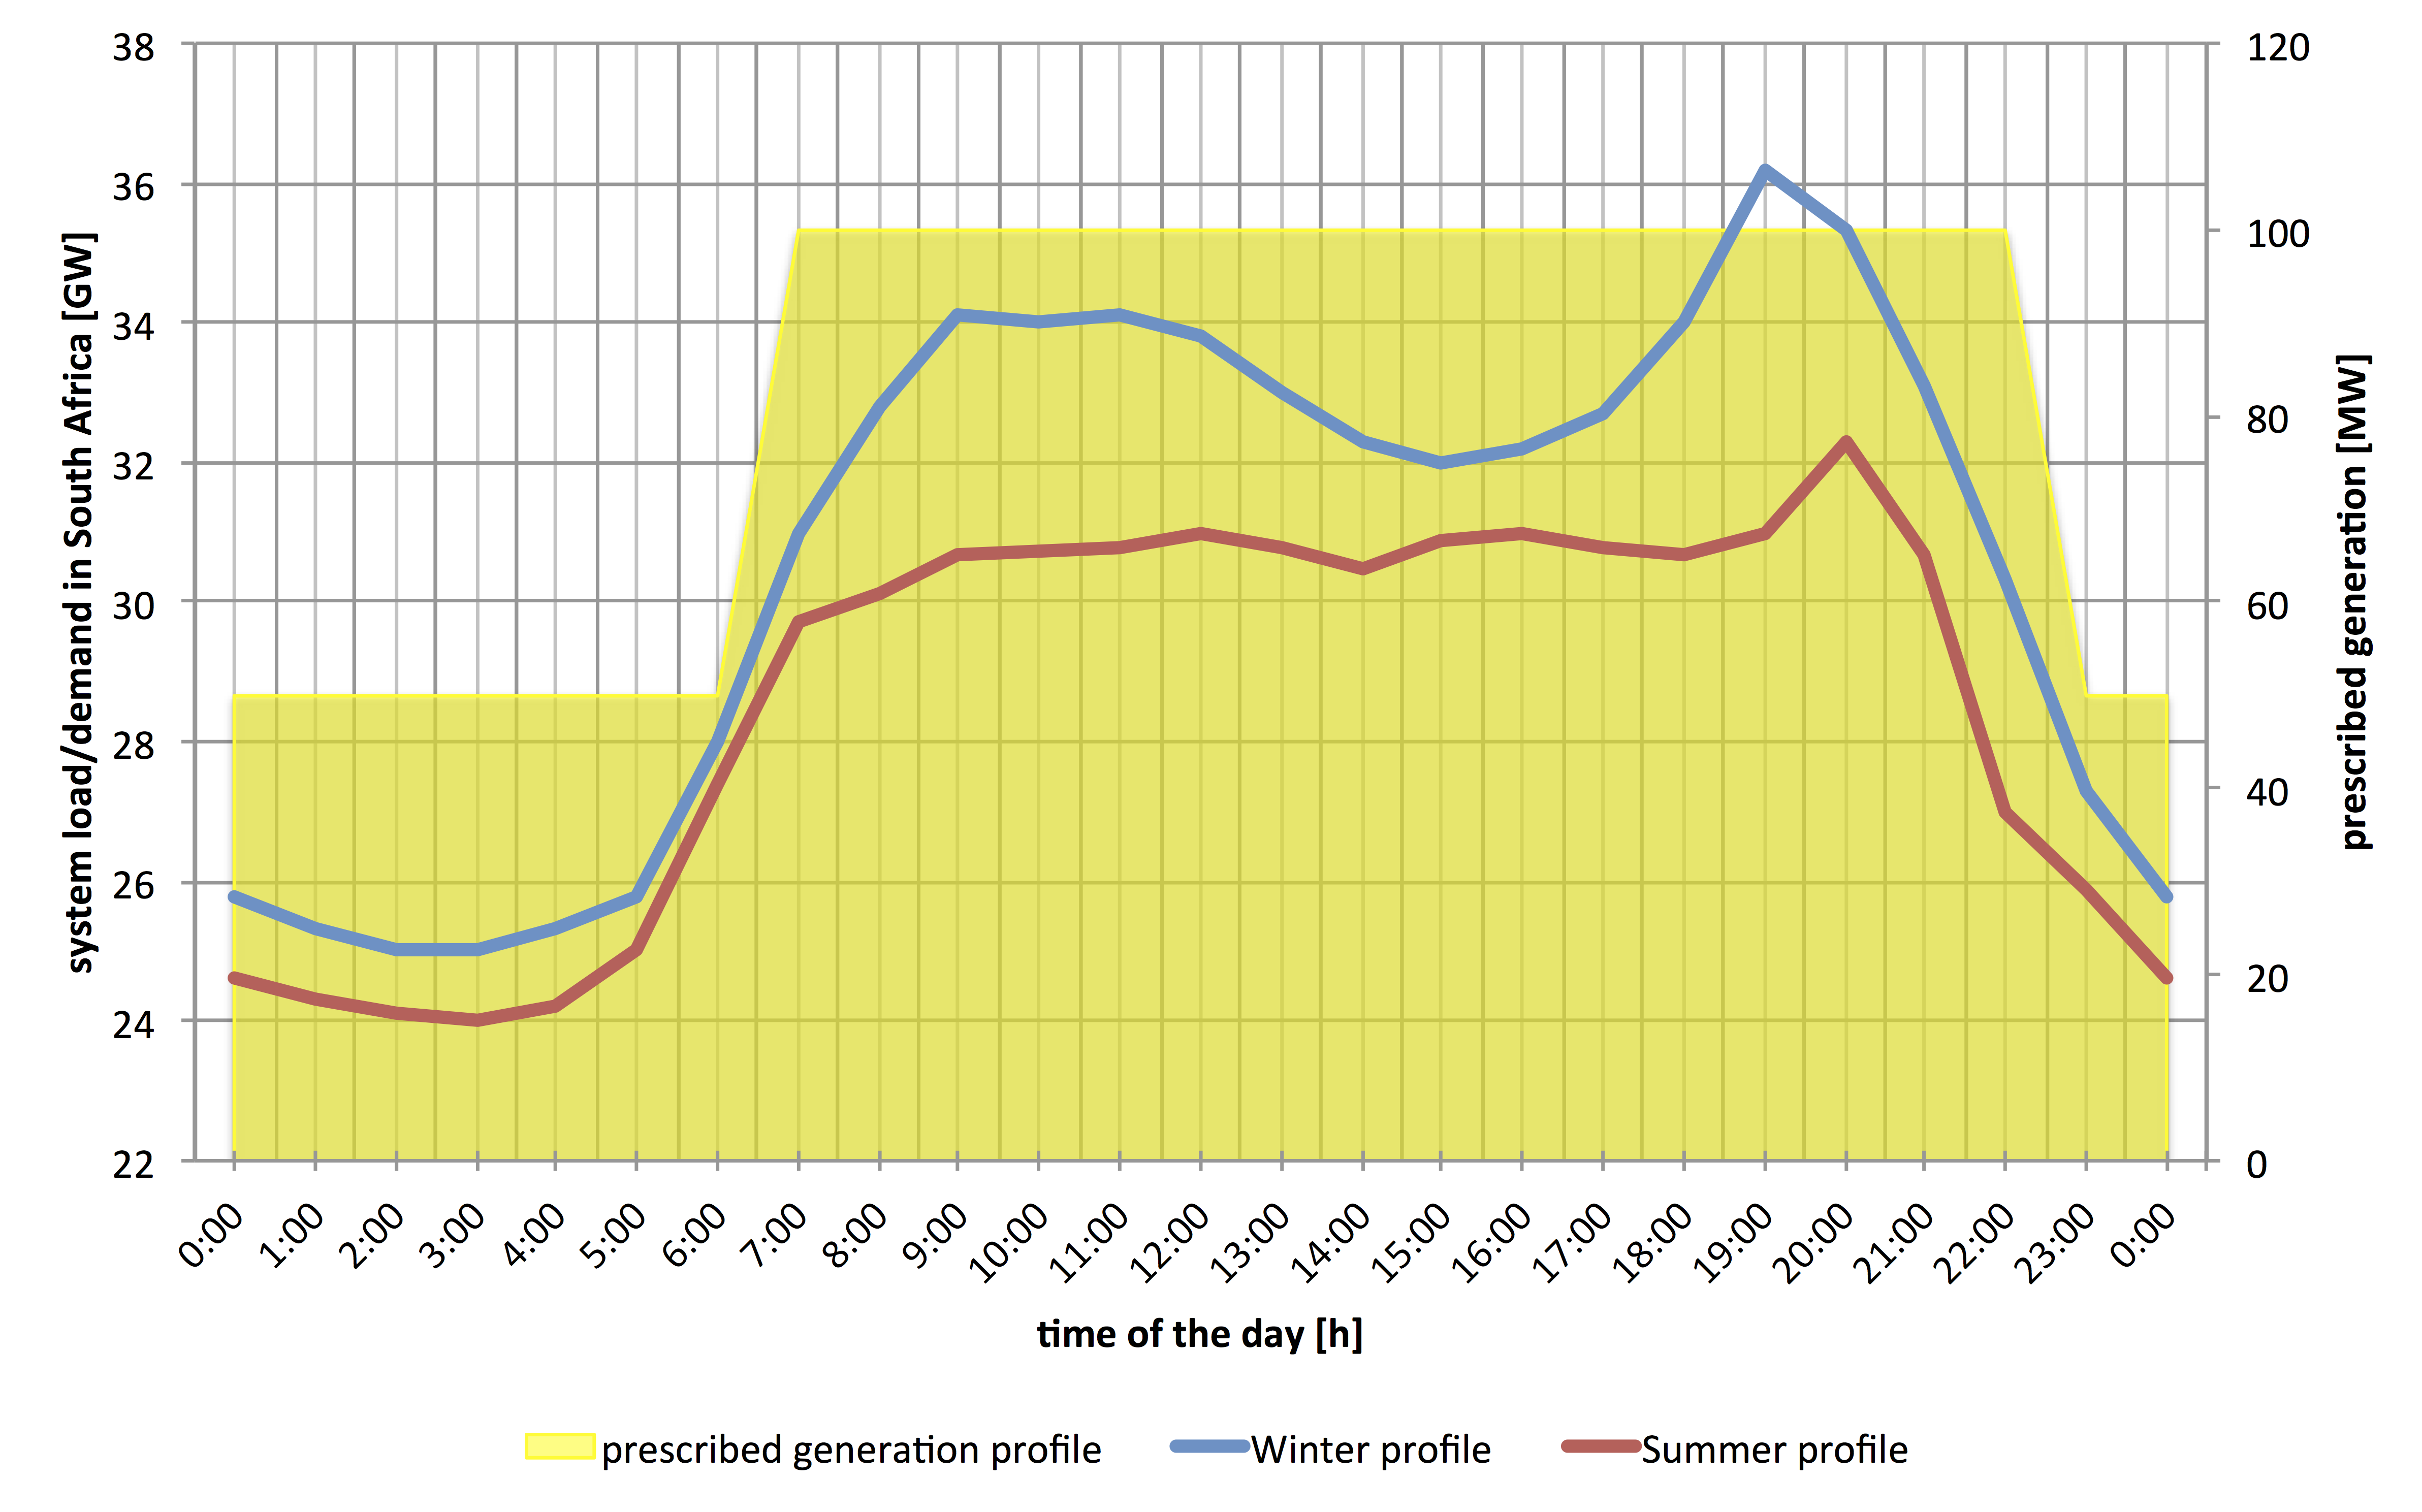
\includegraphics[width=1\linewidth]{FIG/LoadScenarios}
\caption[South Africa daily average system load/demand for summer and winter days, with prescribed generation profile.]{South Africa daily average system load/demand for summer and winter days, with prescribed generation profile.}\label{LoadScenarios}
\end{figure}
%Considering the system load, the supply structure and the point of time by load shedding it is unequivocally that the South African power supply needs adjustable power plants which can support the demand during the evening hours till 22:00 in particular. 
Considering system load, supply structure and load shedding history (Figure~\ref{Load_shedding_sum}) it is clear that adjustable power plants which can meet peak demand during the evening hours are required. 

\begin{figure}[htbp]  
\centering
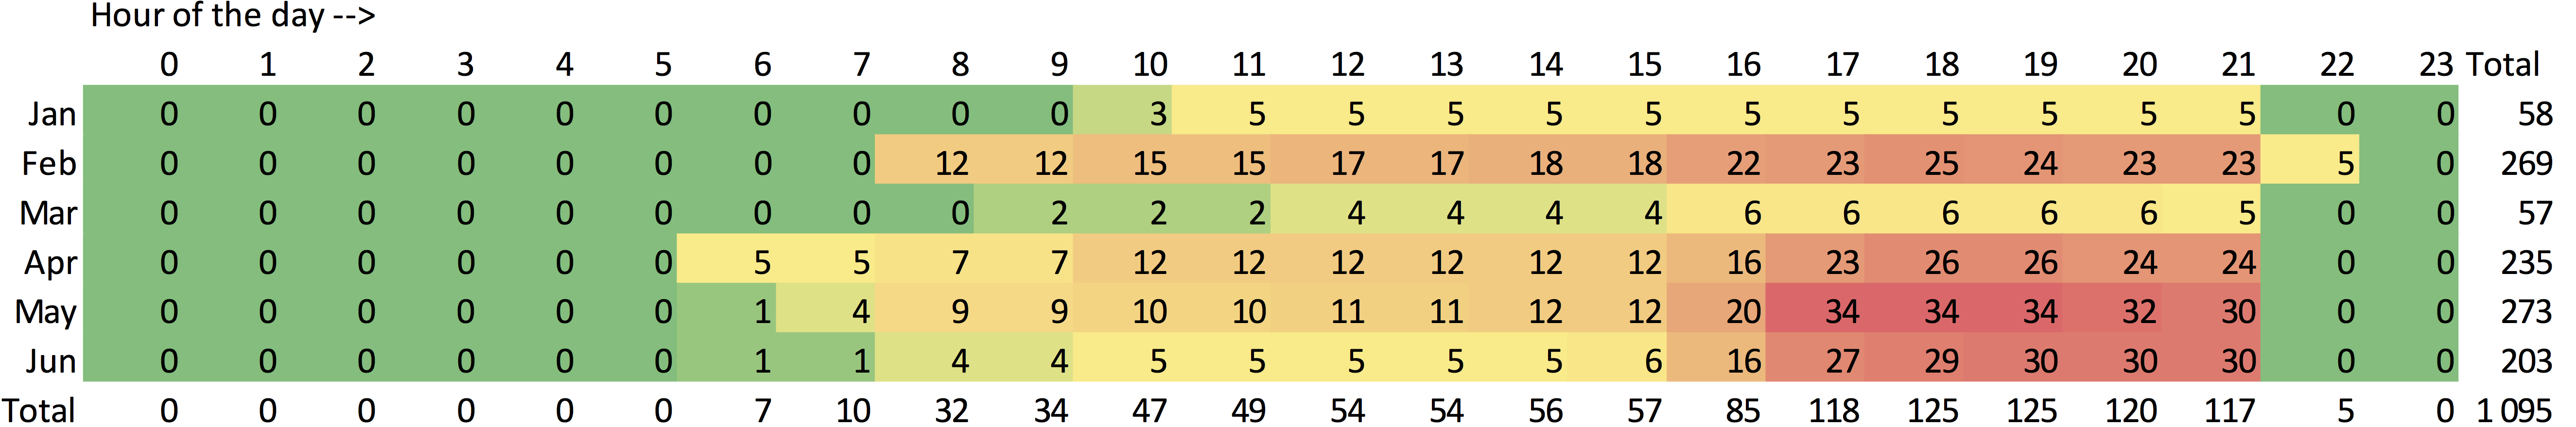
\includegraphics[width=1\linewidth]{FIG/Load_shedding_sum}
\caption[Total unserved energy due to load shedding for all hours per month Jan-Jun 2015 in GWh.]{Total unserved energy due to load shedding for all hours per month Jan-Jun 2015 in GWh \cite{CSIREnergyCentre2015}.}\label{Load_shedding_sum}
\end{figure}

%In order to support the South African power supply were it is needed, the for the comparison selected solar power plants are forced to cover a prescribed generation profile. The solar power plants must operate at full power output of \SI{100}{\mega\watt} from 7:00 to 22:00. When the system demand drops during the night, the plants reduce there output from 22:00 to 7:00 to \SI{50}{\mega\watt}. At a covering of \SI{100}{\percent} of the prescribed generation the solar power plants would produce \SI{711.75}{\giga\watt\hour} per year.
In ensure power is available when needed, the selected solar power plants are forced to meet a prescribed profile. They must operate at a full output of \SI{100}{\mega\watt} from 7:00 to 22:00. When system demand drops during the night, the plants throttle output from 22:00 to 7:00 to \SI{50}{\mega\watt}. At \SI{100}{\percent} coverage of the prescribed profile, the solar plants would produce \SI{711.75}{\giga\watt\hour} per year.

%With consideration to solar energy is depending on weather and seasonal conditions the individual system design must handle \SI{90}{\percent} of the prescribed generation profile and with regard to the PV system whose module efficiency deteriorates over there lifetime it is just defined for the first year of the plants. [Ich verstehe leider nicht was du hier schreibst.]

% It signifies that the power plants are forced to produce more than \SI{640575}{\mega\watt\hour} in the first year.
The individual system design must handle \SI{90}{\percent} of the prescribed profile even when taking weather, seasonal variations and, in the case of PV, declining module efficiency into account. This means that the power plants are forced to produce more than \SI{640575}{\mega\watt\hour} in the first year.

Usually, in feed-in contracts, the deliverable maximum net power output of power plants is fixed. Any overproduction is not covered by such contracts and is not remunerated. In order to generate exploitable and comparable results and considering standard feed-in contracts, the hourly power production is cut to the planned values and thus overproduction is not considered in this analysis. For the purposes of this analysis, a synthetic load profile, called the prescribed profile, is used.

%From the perspective of the power plant the prescribed generation profile can be seen as load. Therefore is in the following thesis with load curve the generation profile described. This load curve is not to be confused with the system load in SA which constantly changes. The load curve is fix defined for this comparison.

%The results of the solar power plant simulations will therefore evaluated and compared by the following quantitative measures:

The solar plant simulations will be evaluated and compared using the following quantitative measures:
\begin{itemize}
\item \textbf{Load curve covering} [\si{\percent}]: The load curve covering (LCC) is an effectiveness measure describing how closely the plant follows the prescribed profile over the full year. It is defined as:
\begin{equation}
\mbox{LCC} = \sum\limits_{t=1}^{8760} \frac{\mbox{prescribed generation at }t\mbox{ in MW}}{\mbox{actual plant net output at }t\mbox{ in MW}} \label{GL_GCC}
\end{equation} 
\item \textbf{Levelized cost of electricity} [USD/\si{\mega\watt\hour}]: The levelized cost of electricity (LCOE) represents the total project life-cycle costs. It is the present value of project costs expressed in USD per megawatt-hour of electricity generated by the system over its life.
\end{itemize}
%These performance and financial parameter are the only relevant indicator for the evaluation in this thesis, other indicators can be seen as supplement. 

These parameters are the only basis for the evaluation in this thesis, others may be seen as supplementary. 

%It must be noted, that there is an important difference between the LCC and the widely-used \emph{capacity factor} (CF). The CF is the ratio of the system's electrical net output in the first year of operation to the nameplate output (CSP) or peak output (PV), which is equivalent to the quantity of energy the system would generate if it operated at its nameplate capacity for every hour of the year \cite{NREL2015a}. The LCC is calculated from the sum value of prescribed generation coverage in each hour of the year. 

Note that there is an important difference between the LCC and the widely-used \emph{capacity factor} (CF). The CF is the ratio of the system's electrical net output in the first year of operation to the nameplate output (CSP) or peak output (PV), which is equivalent to the quantity of energy the system would generate if it operated at its nameplate capacity for every hour of the year \cite{NREL2015a}. The LCC is calculated from the sum value of load coverage in each hour of the year. 


\pagebreak 
\chapter{Large-scale solar power plants}
%Almost all power that we use on our planet comes from the sun. Direct in form of radiation or indirect during wind, water and vegetation. Also the fossil power resources and reserves are stored energy from the sun in from of organic carbon compounds. There are two main technologies for generating electricity out of direct sun radiation. One is the direct conversion of solar irradiance to electrical energy while using photovoltaic. The other is to generate heat and convert it to electrical power. Figure~\ref{OverviewSTP} gives an abstract of the common technologies using direct solar power to generating electric power. This chapter has the focus on large-scale solar power plants and describes parts from both technologies.
Virtually all energy consumed on Earth comes from the sun, whether directly in the form of solar radiation, or indirectly through wind, the water cycle or vegetation. There are two main technologies for generating electricity out of direct solar radiation. One is the direct conversion of solar irradiance to electrical energy via the photovoltaic effect. The other is to first convert that solar irradiance into heat and use that heat to generate electricity. 

%Figure~\ref{OverviewSTP} graphically shows the relationships between common solar technologies for generating generating electric power. This Chapter introduces the solar technologies to cover the in Section~\ref{SystemloadinSA} defined power plant net output load curve. Therefore the technologies which are the focus of this work are highlighted in red.

\begin{figure}[!h] 
\centering
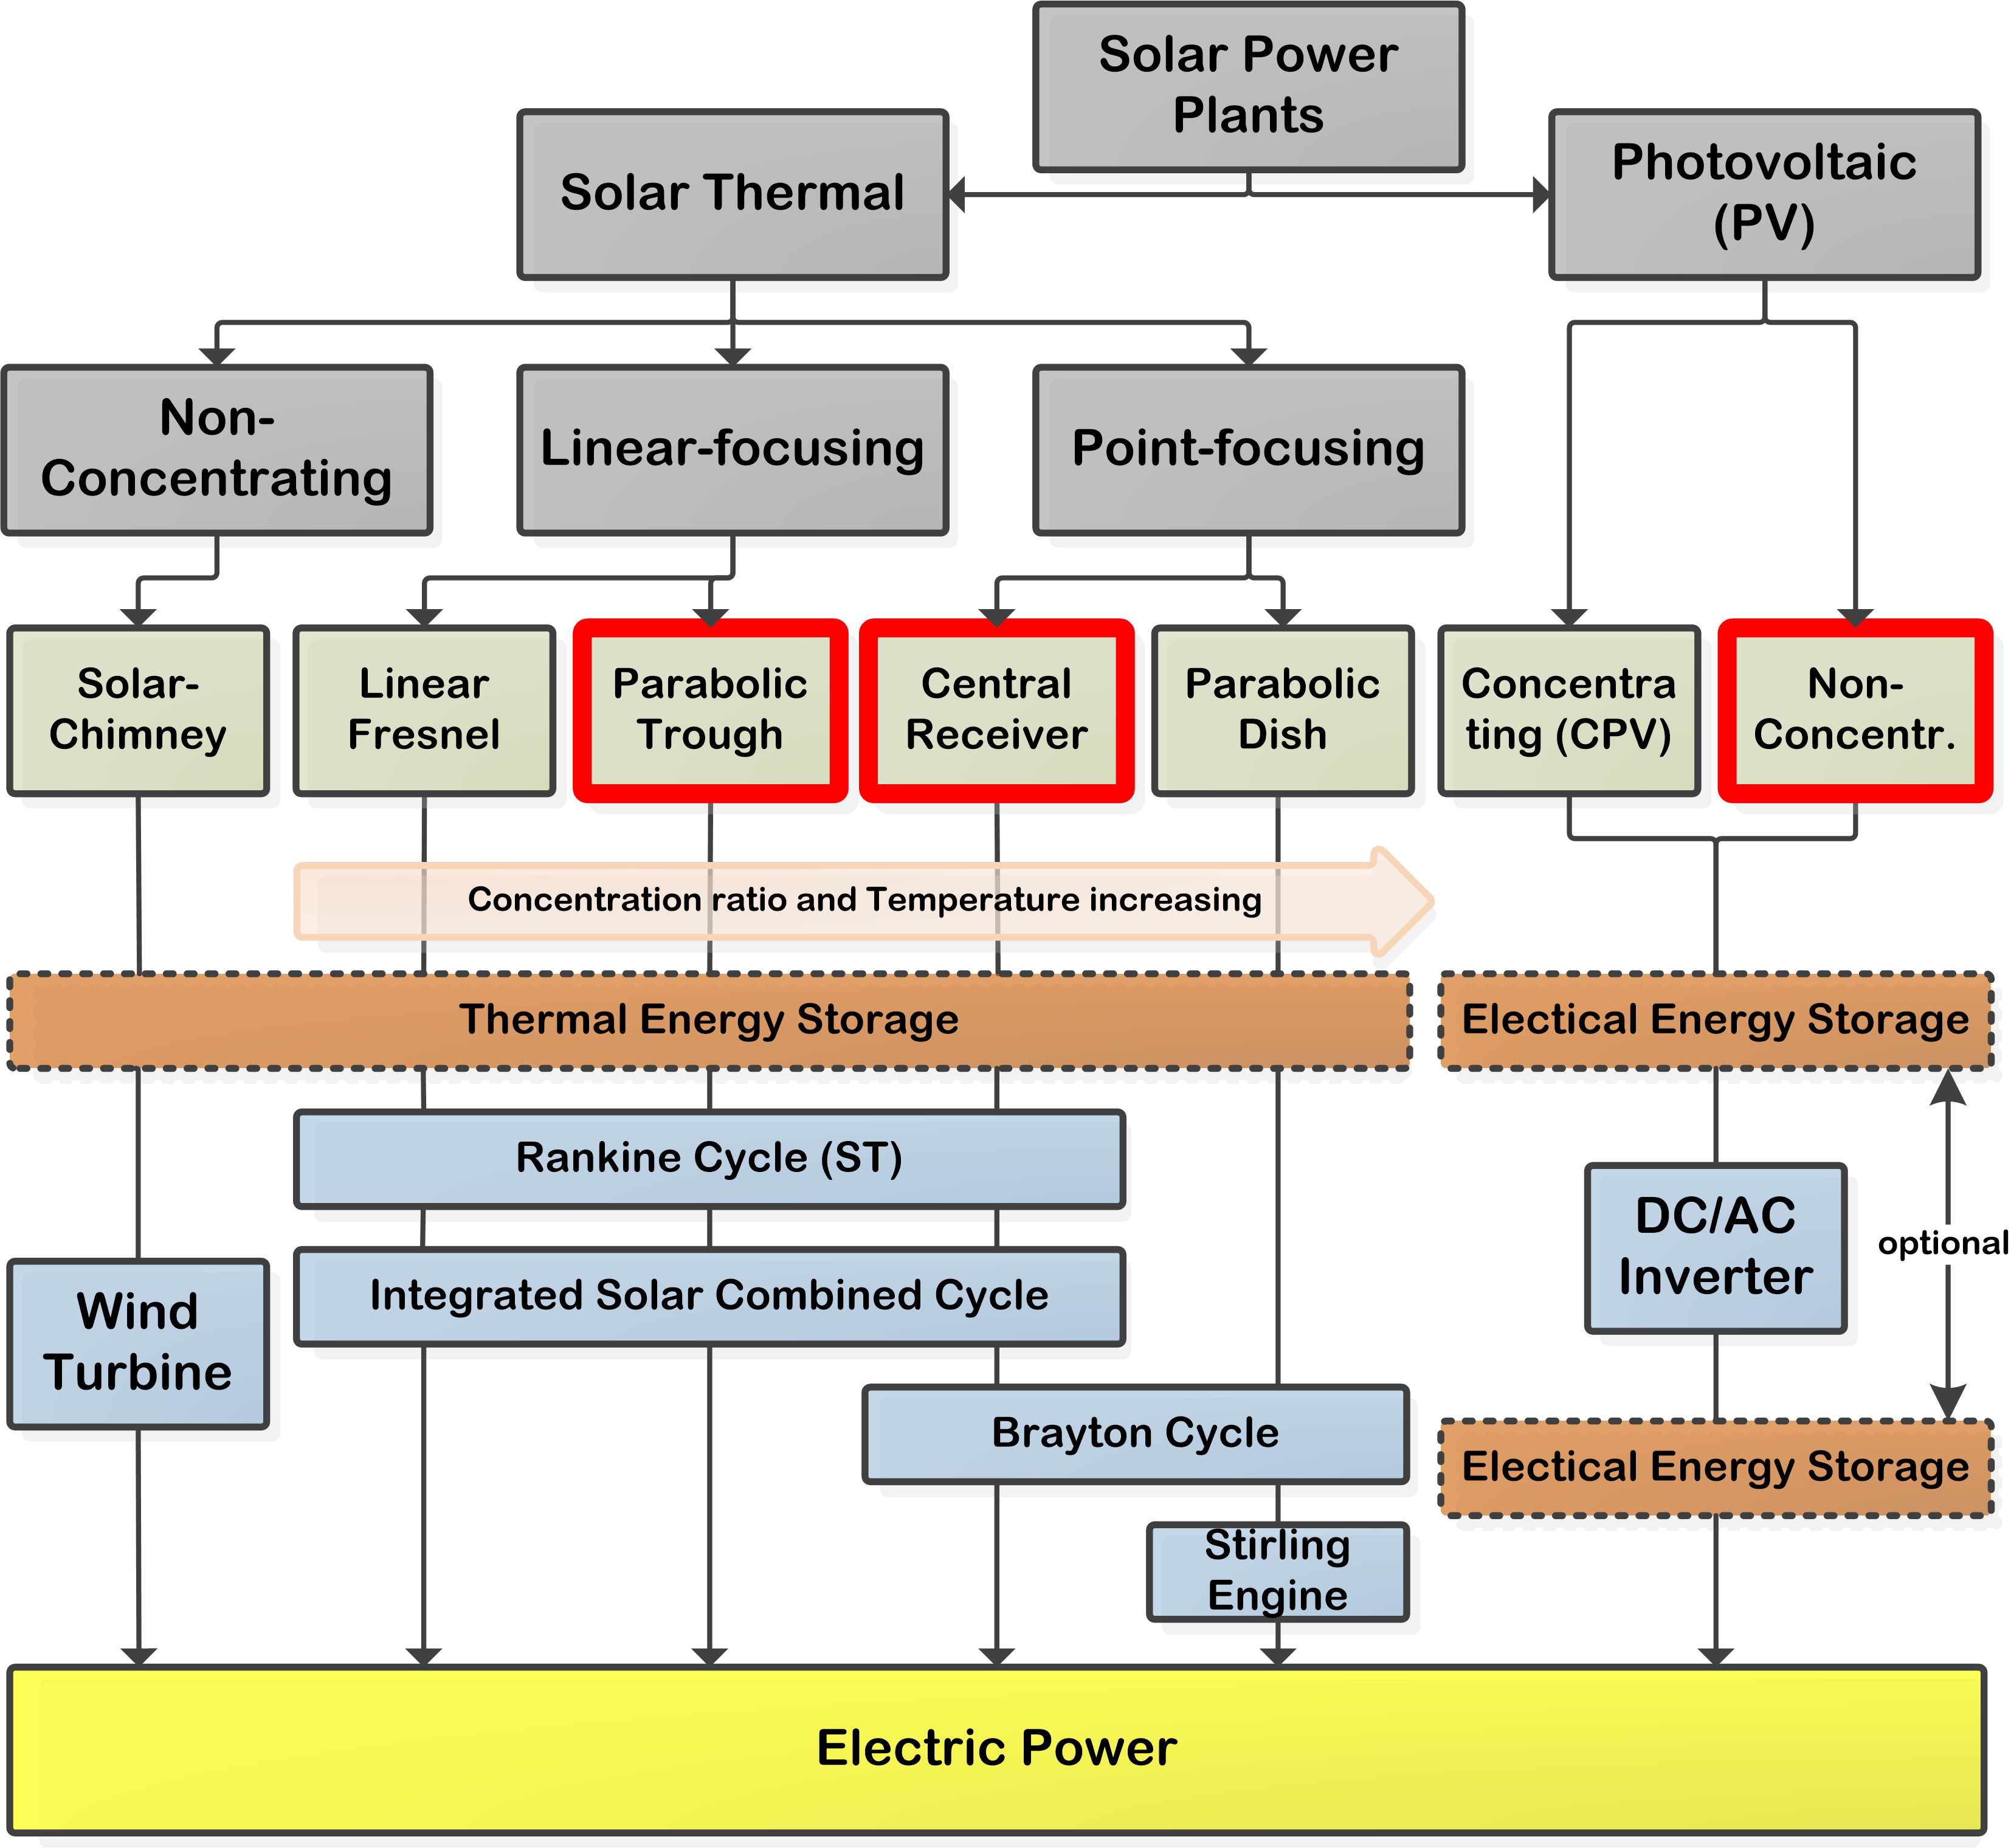
\includegraphics[width=0.8\linewidth]{FIG/OverviewSTP}
\caption[Overview of Solar Power Technologies.]{Overview of Solar Power Technologies.}\label{OverviewSTP}
\end{figure}



%Therefore it is split in the technology fields of large scale concentrated solar power plants (\ref{Large scale concentrated solar power (CSP) plants}) and large scale photo voltaic power plants (\ref{Large scale photo voltaic (PV) power plants}).
%In detail the technologies with a large-scale power plant potential -- parabolic trough, central receiver and non-concentrating photovoltaic -- are described. Also the storage systems for both systems. 
%Therefore it is split in the technology fields of large scale concentrated solar power plants (\ref{Large scale concentrated solar power (CSP) plants}) and large scale photo voltaic power plants (\ref{Large scale photo voltaic (PV) power plants}).
%In detail the technologies with a large-scale power plant potential -- parabolic trough, central receiver and non-concentrating photovoltaic -- are described. Also the storage systems for both systems. 

\section{Large-scale CSP plants}\label{Large scale concentrated solar power (CSP) plants}
%Concentrating solar power (CSP) systems use combinations of mirrors or lenses to concentrate direct beam solar radiation to produce forms of useful energy such as heat, electricity and others. This happens by use of various downstream technologies. Generally the CSP technology includes not only the concentrating solar thermal (CST) technology, but also concentrating photovoltaic (CPV) energy conversion. However, there is no focus on CPV in this thesis. That is why the term CST is put on a level with CSP.
\ac{CSP} systems use combinations of mirrors or lenses to concentrate direct beam solar radiation to produce forms of useful energy such as heat and electricity. This happens by use of various downstream technologies. Generally, \ac{CSP} technology includes not only \ac{CST} technology, but also \ac{CPV} energy conversion. However, \ac{CPV} will not be treated in this thesis.
%A CSP plant comprises four main sub-systems: concentrating system, solar receiver, storage and power block. Also supplementary firing is used in some cases, but is basically not necessary nowadays. A graphic scheme of such a sub-system is shown in Figure~\ref{MainComp}. The separate components are linked together by energy flow in mostly radiation transfer or fluid transport. This chapter describes the function and gives an application overview of the individually components. 
A \ac{CSP} plant comprises four main sub-systems: concentrating system, solar receiver, storage and power block (Figure~\ref{MainComp}). (Supplementary firing was used in the past, but is not necessary nowadays.) The separate components are energetically linked via radiation or fluid transport.
\begin{figure}[!h] 
\centering
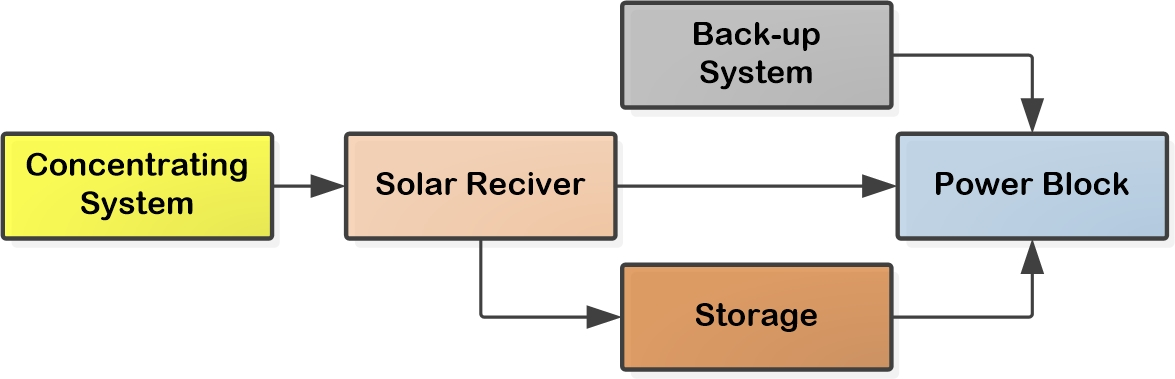
\includegraphics[width=0.85\linewidth]{FIG/MainComp}
\caption[Main components of a CSP plant.]{Main components of a CSP plant.}\label{MainComp}
\end{figure}

%The main advantage of CSP in opposite to other renewable energy producers is the thermal storage to provide power for cloudy days or during night time. Therefore the concentrating system and solar receiver have to produce more thermal energy then the power block can use directly. The ratio of the power capacity of the collector field to the capacity of the power block is defined as Solar multiple (SM). For CSP systems with storage, the number of hours of storage is based on the capacity of the power block. Chapter \ref{Subsection_storage_system} describes technical possibilities and application of thermal storage system for CSP.
The main advantage of \ac{CSP} when compared to other renewable energy producers is its thermal storage, which continues to provide power on cloudy days or at night. This means that the concentrating system and solar receiver must produce more thermal energy then the power block can use directly. The ratio of the output of the collector field to the gross output of the power block is defined as \acfi{SM}. For \ac{CSP} systems with storage, the number of hours of storage is based on the capacity of the power block.

%The solar receiver or concentrating system is eponymously for the main CST technologies. The two most common CSP plant technologies are parabolic trough collector (PTC) and central receiver (CR) systems (also known as solar power towers). Further types of CSP plant are linear Fresnel reflectors (LFR) and parabolic dish. The main difference of the technologies is the concentrating system. Thereof results the differences in optical design, shape of receiver, nature of the transfer fluid and capability to store heat before it is turned into electricity. In systems with a line focus (PTC trough and LFR) the mirrors track the sun along one axis. In those with a point focus (CR and parabolic dish), the mirrors track the sun along two axes. The receiver may be fixed, as in LFR and CR, or mobile as in PTC and parabolic dish systems. An overview of the technologies and there differences in relation to the focus and the receiver  is shown in Table \ref{tbl: CSPtech}.
The two most common \ac{CSP} plant technologies are \ac{PTC} and \ac{CR} systems (also known as solar power towers). Other types include \ac{LFR} and parabolic dish. The main difference between these technologies is the concentrating system, which lead to differences in optical design, shape of receiver, nature of the transfer fluid and capability to store heat before it is turned into electricity. In systems with a line focus (\ac{PTC} and \ac{LFR}) the mirrors track the sun along one axis. In those with a point focus (\ac{CR} and parabolic dish), the mirrors track the sun along two axes. The receiver may be fixed, as in \ac{LFR} and \ac{CR}, or mobile as in \ac{PTC} and parabolic dish systems (see Table \ref{tbl: CSPtech}).

\begin{table}[h!] % Main technologies 
  \centering
  \begin{tabular}{  m{5cm}  m{5cm}  m{5cm}  }
    \hline
    & \textbf{Line focus} & \textbf{Point focus} \\ 
    & Collectors track the sun along a single axis and focus irradiance on a linear receiver. This makes tracking the sun simpler. & Collectors track the sun along two axes and focus irradiance at a single point receiver. This allows for good receiver efficiency at higher temperatures.\\ \hline \hline
    \textbf{Fixed receiver} & &\\

    Fixed receivers are stationary devices that remain independent of the plant's focusing device. This eases the transport of collected heat to the power block.
    &
    \begin{minipage}[t]{5cm}
      \centering
	 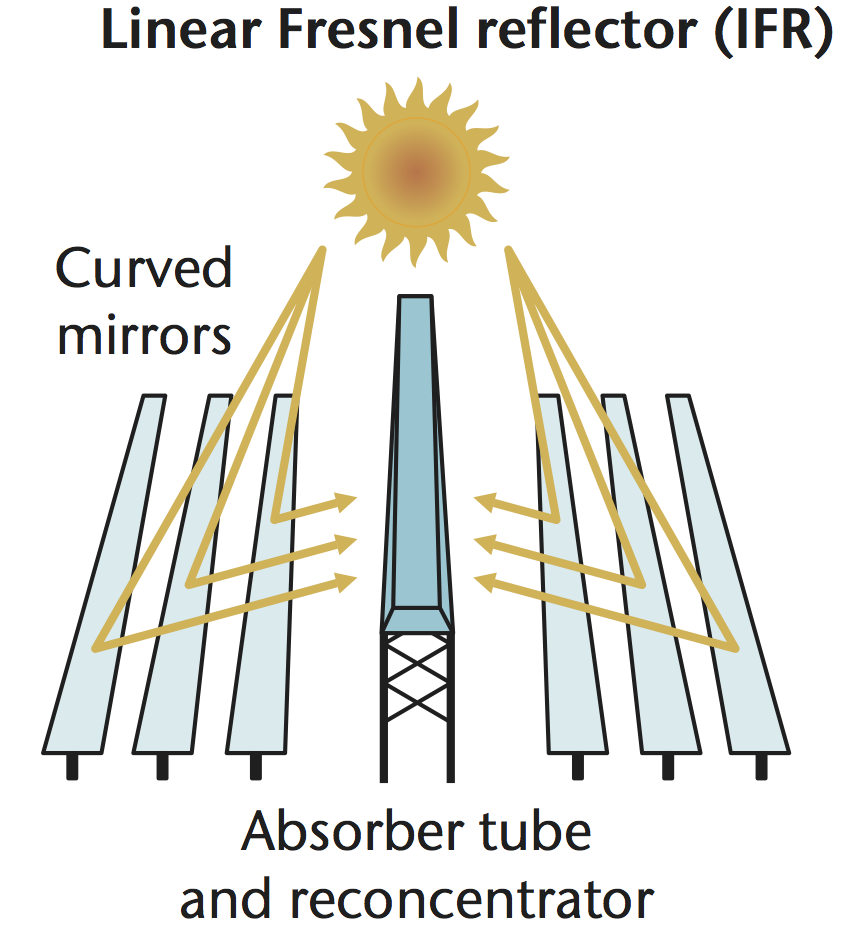
\includegraphics[height=55mm]{FIG/SUM/LF}
    \end{minipage}
    & 
    \begin{minipage}[t]{5cm}
      \centering
	  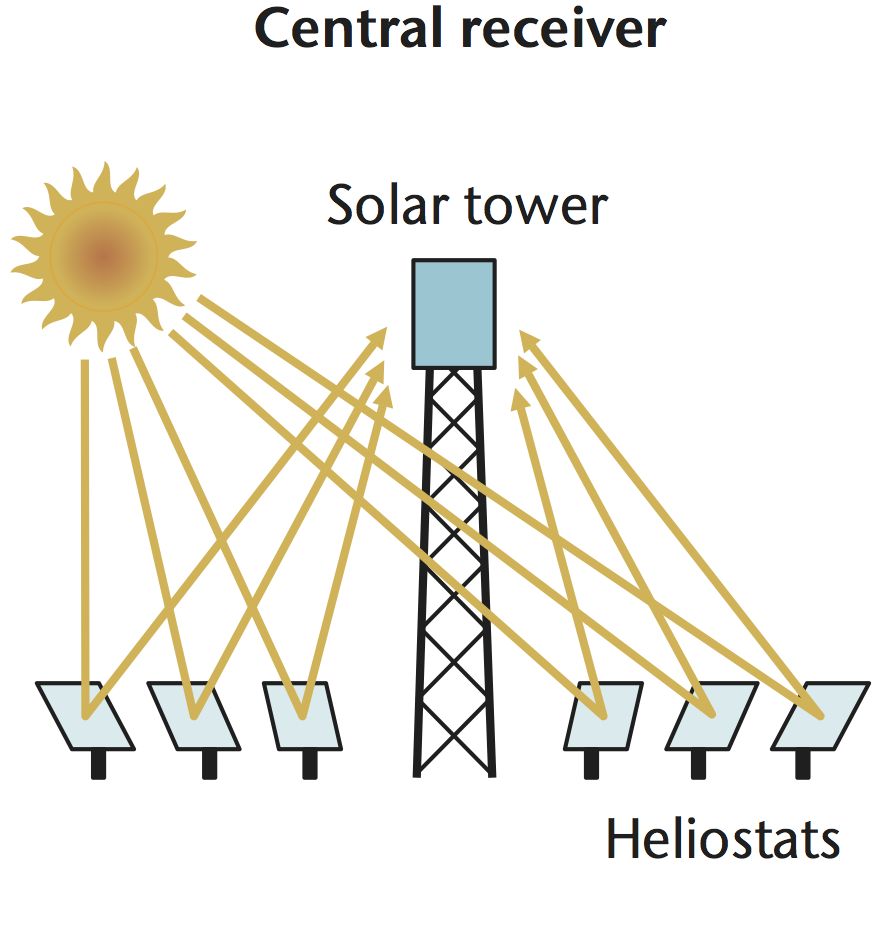
\includegraphics[height=55mm]{FIG/SUM/ST}
    \end{minipage}
    \\ \hline
    \textbf{Mobile receiver} & & \\
    Mobile receivers move together with the focusing device. In both line focus and point focus designs, mobile receivers collect more energy.
    &
    \begin{minipage}{5cm}
      \centering
	  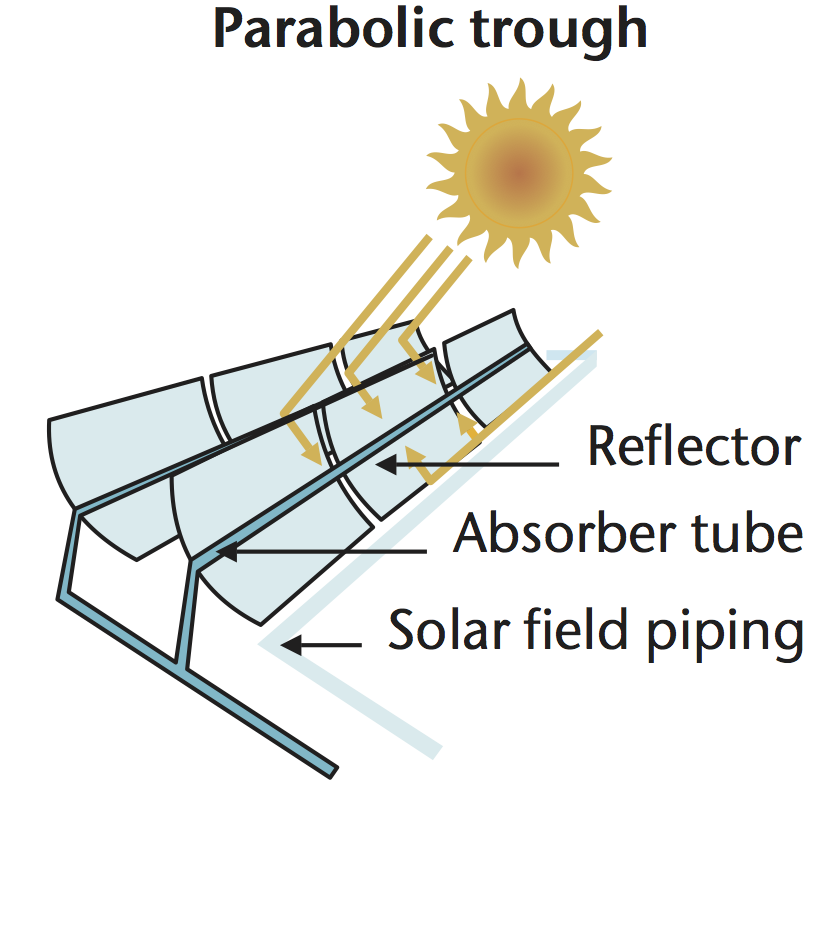
\includegraphics[height=55mm]{FIG/SUM/PT}
    \end{minipage}
    & 
    \begin{minipage}{5cm}
      \centering
	  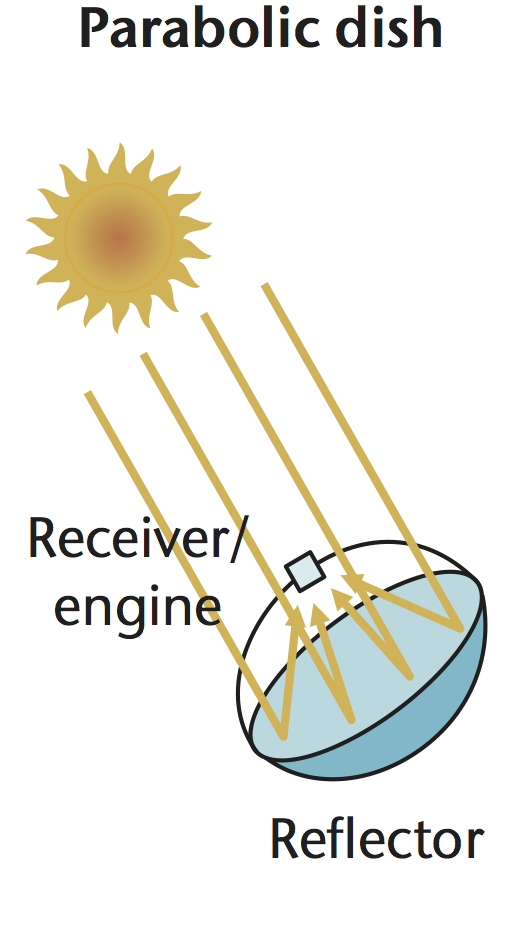
\includegraphics[height=55mm]{FIG/SUM/PD}
    \end{minipage}    
    \\ \hline
  \end{tabular}
  \caption[CSP technology families.]{CSP technology families \cite{IEA2014c}.}\label{tbl: CSPtech}
\end{table}


%As mentioned above is main difference between the CSP technology families how they concentrate the solar radiation. This strongly affects their overall efficiency. The parabolic dish has the best annual optical efficiency (about 90\%) because the concentrator axis is always parallel to the sun rays. The worst (about 50\%) is observed for linear Fresnel systems because of poor performance in the morning and in the evening. Intermediate values (65-75\%) are obtained for parabolic trough and tower systems. For each family the actual efficiency varies with the location, the time of day and the season of the year. \cite{EASAC2011} 
The main difference between the \ac{CSP} technology families is in how they concentrate the solar radiation, which affects their overall efficiency. The parabolic dish has the best annual optical efficiency (\sim\SI{90}{\percent}) because the concentrator axis is always parallel to the sun's rays. The worst (\sim\SI{50}{\percent}) is observed for \ac{LFR} systems because of poor performance at low solar irradiation angles. Intermediate efficiencies (\SIrange{65}{75}{\percent}) are obtained for \ac{PTC} and \ac{CR} systems. For each family, actual efficiency varies with location, time of day and season \cite{EASAC2011}.

%The capacity range of an CSP-plant is also strongly affected by the concentration ratio. The most common definition of concentration ratio is the ratio of the area of reflector aperture ($A_a$) to the area of receiver ($A_r$). The area concentration is:
The capacity range of a \ac{CSP} plant is also strongly affected by the concentration ratio, which is defined as the ratio of the area of reflector aperture ($A_a$) to the area of receiver ($A_r$):
\begin{align}
C=\frac{A_{a}}{A_{r}} \label{GL_concentration}
\end{align}

%The concentration ratio from Equation \ref{GL_concentration} has an upper limit that depends on whether the concentration is a three dimensional (point focus) concentrator such as a parabolic dish and central receiver solar tower or a two-dimensional (linear focus) concentrator such as parabolic trough and linear Fresnel reflector. The maximum concentration ratio is based on the second law of thermodynamics applied to radiative heat exchange between the sun and the receiver. The maximum possible concentration ratio for circular concentrators is 45~000, and for linear concentrators is the maximum 212. \cite{Duffie2013}
The concentration ratio from Equation \ref{GL_concentration} has an upper limit that depends on whether the concentration is a three-dimensional (point focus) concentrator such as a parabolic dish or \ac{CR} systems, or a two-dimensional (linear focus) concentrator such as a \ac{PTC} or \ac{LFR} systems. The maximum concentration ratio is based on the second law of thermodynamics applied to radiative heat exchange between the sun and the receiver. The maximum possible concentration ratio for circular concentrators is \num{45000}, for linear concentrators it is \num{212} \cite{Duffie2013}.

\begin{table}[h!]  
  \centering
	\begin{tabular}{  p{3.0cm}  C{2.0cm}  C{2.2cm}  C{2.0cm}  C{2.0cm}  C{2.0cm}} 
\hline
\textbf{Technology} & \textbf{Capacity range} (\si{\mega\watt}) & \textbf{Concent- ration} & \textbf{Peak system efficiency} (\si{\percent}) & \textbf{Annual system efficiency} (\si{\percent}) & \textbf{Thermal cycle efficiency} (\si{\percent}) \\ \hline \hline
Parabolic trough & \numrange{10}{280}& \numrange{70}{100} & \num{21} & \numrange{10}{16} & \numrange{35}{42} ST  \\ \hline
Fresnel reflector & \numrange{10}{200} & \numrange{25}{100} & \num{20} & \numrange{9}{13} & \numrange{30}{42} ST  \\ \hline
Solar tower & \numrange{10}{200} &  \numrange{300}{1000} & \num{23} & \numrange{8}{23} & \numrange{0}{45} ST  \\ \hline
Dish-Stirling & \numrange{0.01}{0.4} & \numrange{1000}{3000} & \num{29} 29 & \numrange{16}{28} & \numrange{30}{40} \\ \hline
\multicolumn{2}{l}{ST = Steam Turbine}
\end{tabular}
\caption[Performance characteristics of CSP technology families.]{Performance characteristics of CSP technology families \cite{Pitz-Paal.2013} \cite{AbengoaSolar2013a}.}\label{tbl: CSPCharacteristics}
\end{table}

%But actually the technical implementation of concentration ratio is the main parameter for the capacity range of a CSP plant. Table~\ref{tbl: CSPCharacteristics} gives an overview of some of the performance characteristics of the concentrating solar power concepts. More details are listed in Annexure I, Part A, Figure~\ref{CSPOverview1} on Page~\pageref{CSPOverview1} and Figure~\ref{CSPOverview2} on Page~\pageref{CSPOverview2}. PTC, LFR, and CR can be coupled to steam cycles of 10-280~MW electric capacity (and more), with thermal cycle efficiencies of 30-45~\%. Also the applies for stirling engines which are coupled to dish systems have similar efficiency ranges. The conversion efficiency of the power block remains essentially the same as in conventional-fired power plants. The annual system efficiency are the net power generation over incident beam radiation. They are lower than the conversion efficiencies of conventional steam or combined cycles, because they include the conversion of solar radiative energy to heat within the collector and the conversion of the heat to electricity in the power block. \cite{Pitz-Paal.2013}
% I do not understand the intended meaning of this sentence:
%But actually the technical implementation of concentration ratio is the main parameter for the capacity range of a CSP plant.

Table~\ref{tbl: CSPCharacteristics} gives an overview of performance characteristics. \ac{PTC}, \ac{LFR}, and \ac{CR} systems can be coupled to steam cycles of \SIrange{10}{280}{\mega\watt} electric capacity (and more), with thermal cycle efficiencies of \SIrange{30}{45}{\percent}. Stirling engines that are coupled to dish systems have similar efficiency ranges. The conversion efficiency of the power block is consistent with conventional power plants. The annual system efficiency is the net power generation over incident beam radiation. This is lower than the conversion efficiencies of conventional steam or combined cycles because it includes include the conversion of solar radiative energy to heat within the collector and the conversion of the heat to electricity in the power block \cite{Pitz-Paal.2013}.

\begin{figure}[!h] 
\centering
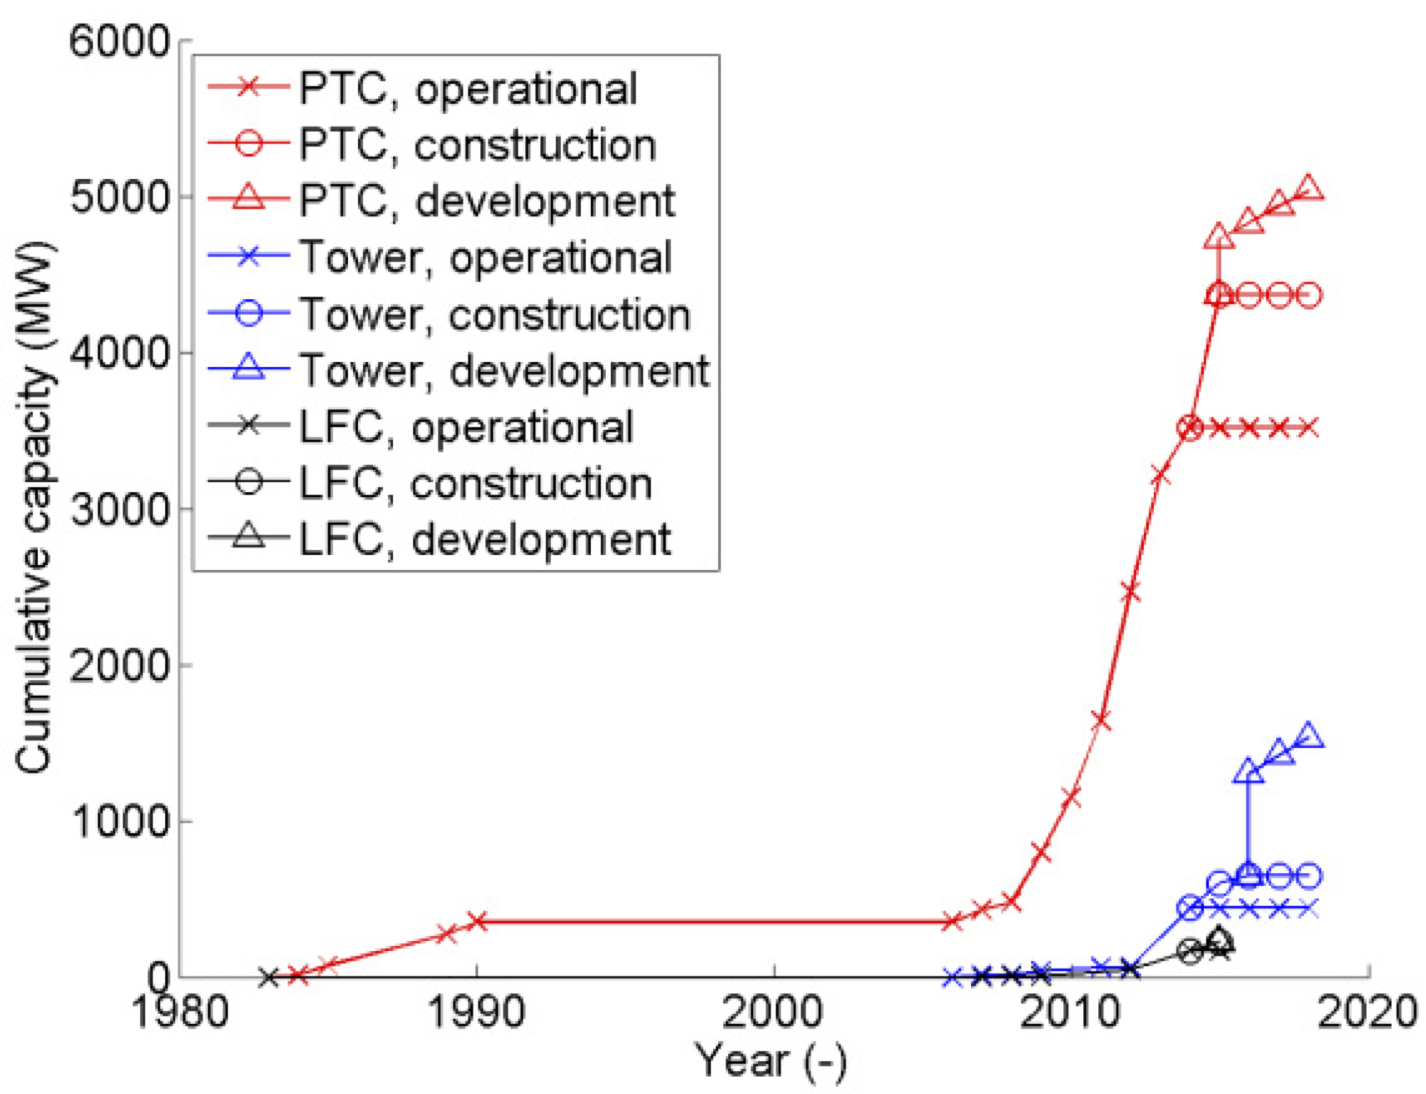
\includegraphics[width=0.65\linewidth]{FIG/CSP_technology_development}
\caption[Historical development of CSP technologies.]{Historical development of CSP technologies \cite{Abbas2015}.}\label{CSP_technology_development}
\end{figure}

%The development of the actual CSP plant technology goes back in the 1970's and 1980's, which is a consequent from the first two Oil crises. Figure~\ref{CSP_technology_development} shows the historical development of PTC, LFR in the Figure called linear Fresnel collector (LFC) and the CR (tower). The parabolic dishes have not succeeded at all and aren't shown here. The reason for that is mainly due to the high structural costs of moving an large diameter dish with two-axes tracking. One might observe that the predominant technology is the PTC, with an installed capacity well above 3~GW. CR have started the exponential development some years later compared to PTC, which explains why the operational installed capacity is much lower. Similarly the development for LFR have started even later, which drives to the lowest installed capacity of the three technologies. The difference in the timing of the three successful technologies is very influenced by the CSP development in its first golden period, the 1980's. In such period important central tower prototypes were built in USA (Solar One, Solar Two, CESA-1) and a 365~MW PTC solar plant was installed in the Mojave Desert. When the oil prices dropped at the end of the second oil crises interest on renewable energies was lost until the last decade. 
The development of the \ac{CSP} technology began in earnest in the 1970s, a consequence of the first two oil price shocks. Figure~\ref{CSP_technology_development} shows the historical development of \ac{PTC} and \ac{LFR} (called linear Fresnel collector (LFC) here) technologies and the \ac{CR} (tower). Parabolic dish systems have not been widely adopted and are not shown here; this is mainly due to the high costs associated with moving a large diameter dish with two-axis tracking. The predominant technology remains \ac{PTC}, with an installed capacity well above \SI{3}{GW}. The first commercial-scale \ac{CR} systems were built decades later, and that of \ac{LFR} systems later still; the operational installed capacity is proportional to the number of years the technology has been available. In the 1980s, important \ac{CR} prototypes were built in the USA (\emph{Solar One}, \emph{Solar Two}, \emph{CESA-1}) and the in total \SI{365}{\mega\watt} \ac{PTC} solar plants \emph{SEGS I-IX} was built at Kramer Junction in the Mojave Desert. When oil prices dropped after the second oil crisis, interest in renewable energies waned and did not return until the beginning of the new millenium. 

%With regard to the past development in the different CSP technology deals this theses with the PTC as well as with the CR technology. The most relevant facts to the separate technologies and there technical components are described in the following shortly in order to describe there technical possibilities to cover the prescribed load curve. 

This work treats \ac{PTC} and \ac{CR} technology. Relevant features of these technologies and their technical components are described here briefly, as they have implications for a plant's ability to meet the prescribed load curve. 

\subsubsection{Overview of CR system technology}
%As it was mentioned above, a CSP system basically consists of five main part, namely concentration system, solar receiver, storage, power block and heat transfer fluid (HTF) system. Which are in case of a CR power plant a solar field (heliostat field) consisting by several two-axis tracking heliostats, a thermal receiver which is mounted on a tower, a thermal storage usually using molten salt or a steam accumulator (depending on HTF), a power block mostly based on Rankine cycle technology and steam or molten salt as HTF. Figure~\ref{towerdirecttwotank} shows the simplified CR power plant scheme of the demonstration project \emph{Solar Two} (1995-2001). 

A \ac{CSP} system consists of five main components: the concentration system, solar receiver, storage, power block and \acf{HTF} system. In the case of a \ac{CR} plant, these are, respectively, a solar field (heliostat field) consisting by several two-axis tracking heliostats, a thermal receiver which is mounted on a tower, thermal storage usually using molten salt or a steam accumulator (depending on \ac{HTF}), a power block based on Rankine cycle technology, and steam or molten salt as \ac{HTF} (Figure~\ref{towerdirecttwotank}).

%Currently CR systems can be separated by two receiver types, external (tube) receiver and cavity receiver \cite{Hoffschmidt2014}. The \emph{Solar Two} project used a external receiver to heat up molten salt at a top temperature of \SI{565}{\celsius} \cite{Reilly2001}. This project concept was the basic research for the current state of art in CR power plants using molten salt as HTF. Typical solar heat fluxes in this type of receiver are up to \SI{1}{\mega\watt\per\square\metre} \cite{Pitz-Paal.2013}. Cavity receiver are currently mostly used in connection with direct saturated or super heated steam production, which is not easy to store over longer duration and therefore not suitable for the defined load profile in thesis \cite{Hoffschmidt2014,Steinmann2015}.

\ac{CR} systems can be differentiated by type, external (tube) receiver and cavity receiver \cite{Hoffschmidt2014}. The \emph{Solar Two} project used a external receiver to heat up molten salt to \SI{565}{\celsius} \cite{Reilly2001}. This concept is the state of the art for CR plants using molten salt as \ac{HTF}. Typical solar heat fluxes in this type of receiver are up to \SI{1}{\mega\watt\per\square\metre} \cite{Pitz-Paal.2013}. Cavity receivers are primarily used in connection with direct saturated or super-heated steam production, which is not easy to store over longer duration and therefore not suitable for the prescribed load profile \cite{Hoffschmidt2014,Steinmann2015}.


\begin{figure}[htbp]  
\centering
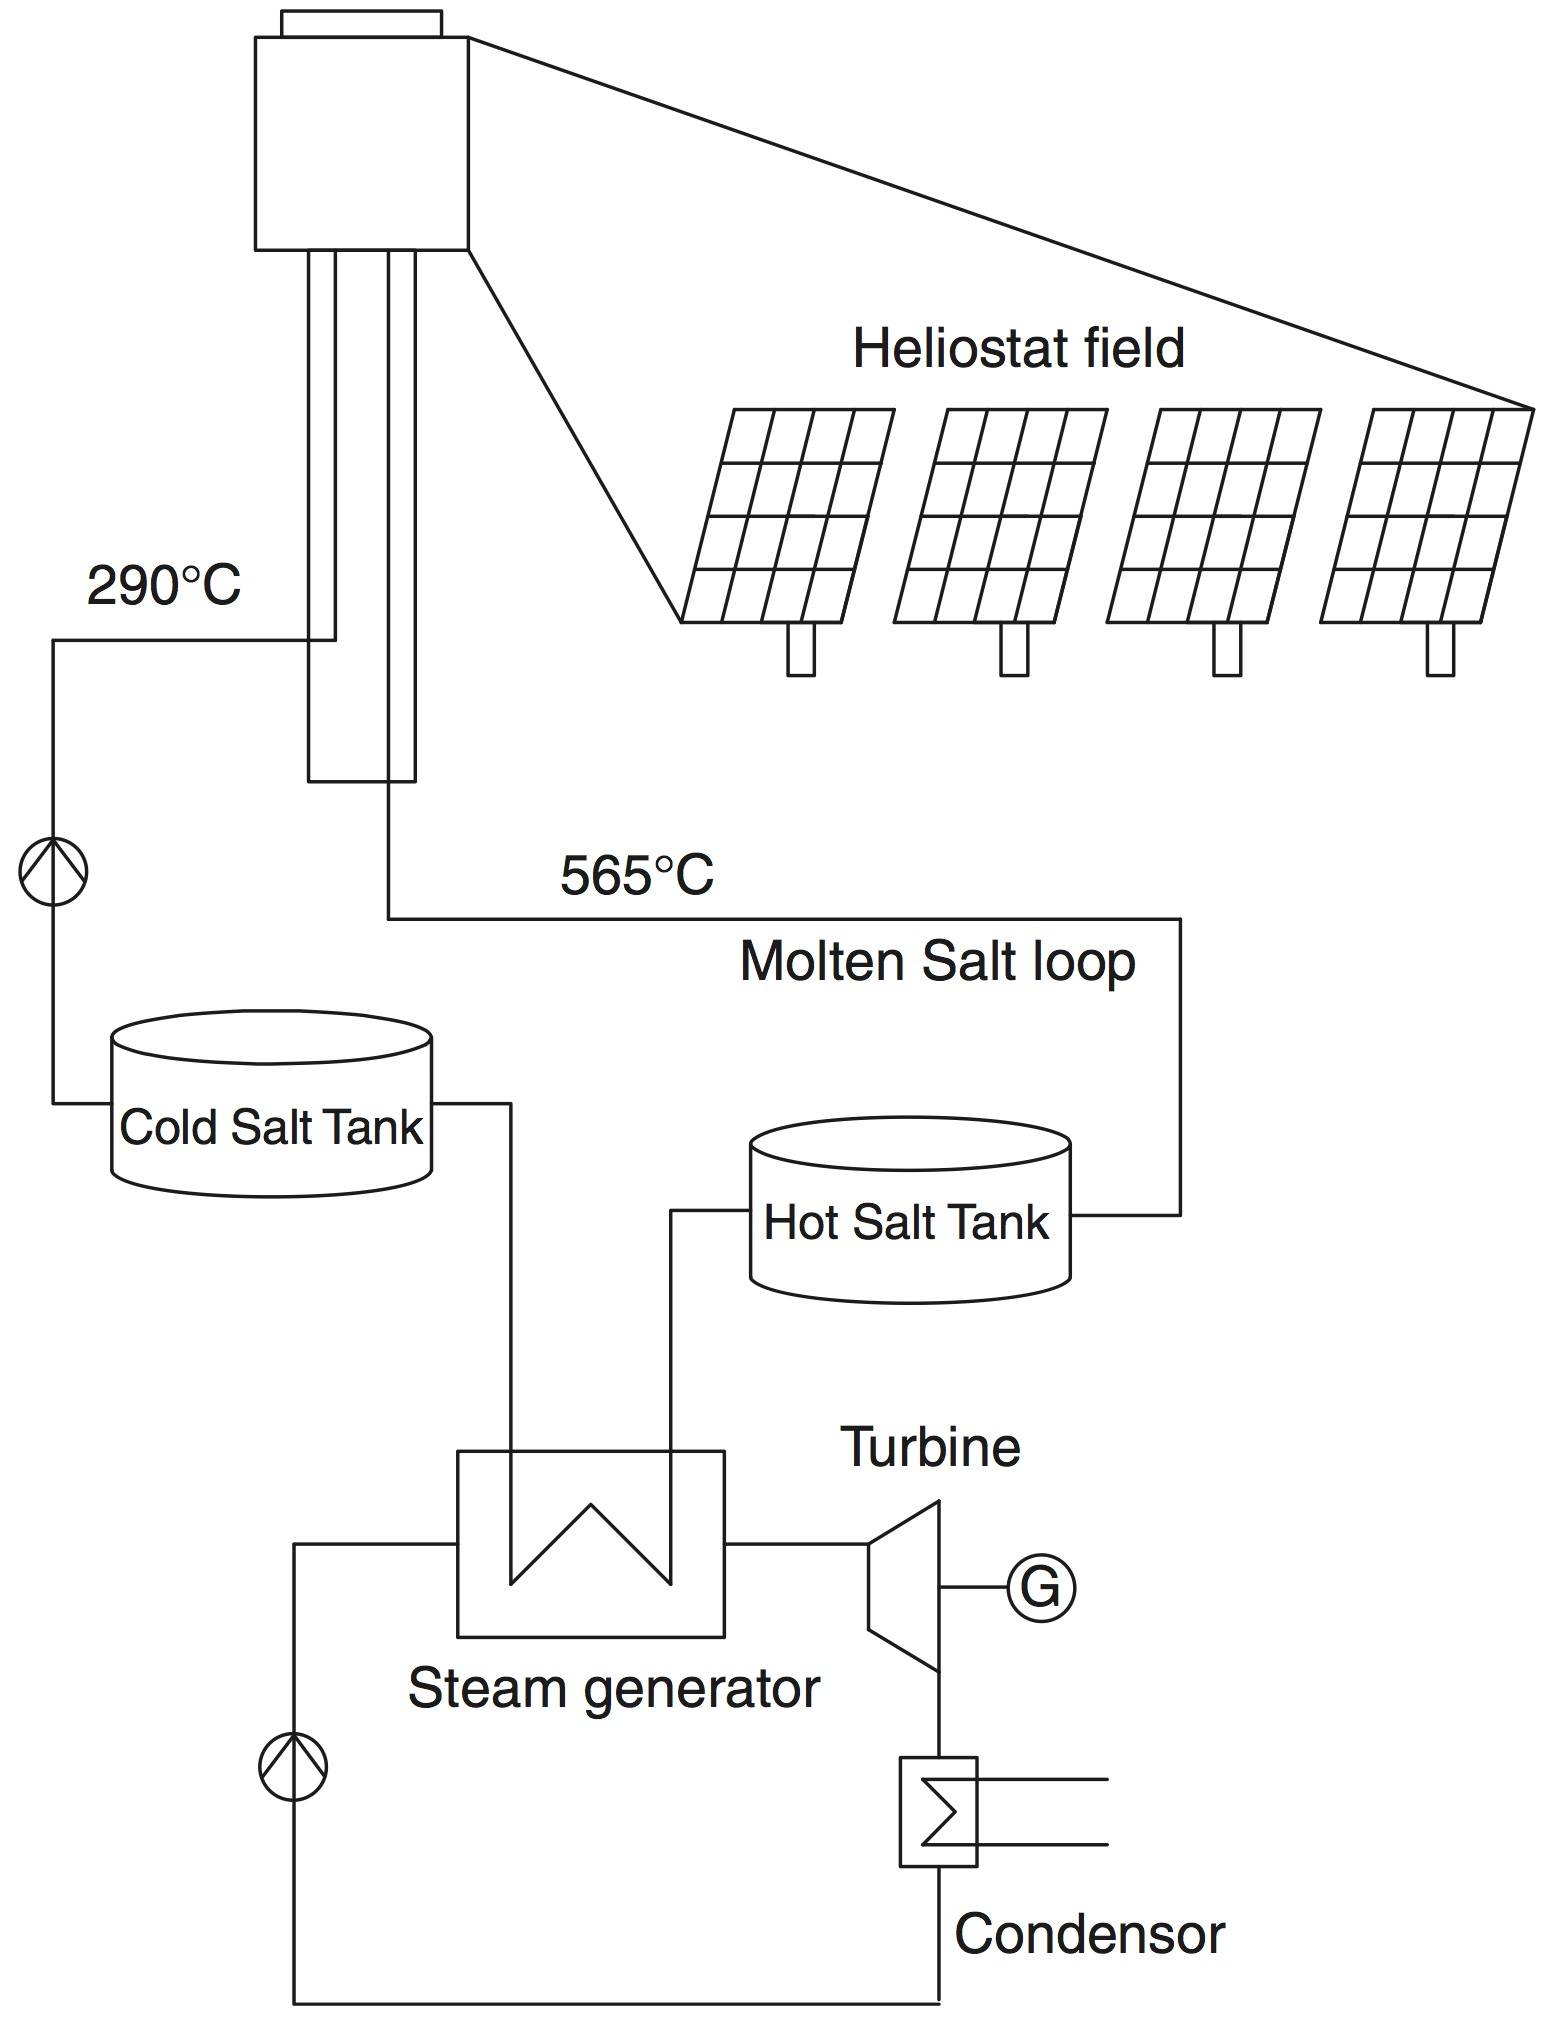
\includegraphics[width=0.45\linewidth]{FIG/towerdirecttwotank}
\caption[Simplified scheme of \emph{Solar Two} \ac{CR} power plant with direct storage of molten salt used as heat transfer fluid.]{Simplified scheme of \emph{Solar Two} \ac{CR} power plant with direct storage of molten salt used as heat transfer fluid \cite{Richter2013}.}\label{towerdirecttwotank}
\end{figure}

%Classical two-axis tracking heliostats design is dominated by mirrors brought into position by steel structures and drives that guarantee high accuracies underwind loads and thermal stress situations \cite{Alexopoulos2013}. The reflective surface of can therefore reach sizes from \SIrange{1.1}{320}{\square\metre} \cite{Blackmon2012,Tyner2014}. There is not really one specific size pushed through for commercial scale application, but one of the marked leader \emph{Abengoa Solar} currently uses \SI{140}{\square\metre} heliostats for CR projects in SA \cite{Abengoa2014}.

Classical two-axis tracking heliostat design consists of mirrors held in position by steel structures and drives that guarantee high accuracies under wind loads and thermal stress situations \cite{Alexopoulos2013}. The reflective surface area is \SIrange{1.1}{320}{\square\metre} \cite{Blackmon2012,Tyner2014}. No specific sizes have established themselves for commercial scale application, but a market leader, Abengoa Solar, is using \SI{140}{\square\metre} heliostats for CR projects in South Africa \cite{Abengoa2014}.

%The main advantage for using molten salt as HTF is the comparatively high thermal range and its good manageability storage characteristics. Molten salt in CR systems can be stored directly in two tanks as its shown in the scheme. For the storage capacity, the thermal range of the receiver temperature and the storage volume is decisive. The storage capacity is usually measured in hours of storage capacity at full load turbine output. Commercial direct molten salt thermal energy storages (TES) in CR systems currently reaches storage capacities of \SI{17.5}{\hour} \cite{NREL2015b}.
The main advantage of molten salt as \ac{HTF} is the comparatively high thermal range and its favorable storage characteristics. Molten salt in \ac{CR} systems can be stored directly in two tanks. Storage capacity is determined by the temperature range of the receiver and the storage volume. The storage capacity is usually measured in hours of storage capacity at full load turbine output. Commercial direct molten salt \ac{TES} in \ac{CR} systems currently reaches storage capacities of \SI{17.5}{\hour} \cite{NREL2015b}.

\subsubsection{Overview of PTC system technology} 
%The concentration system of a PTC plant consist out of parabolic shaped mirrors which is focusing the solar beam on to a receiver tube in the focus point of the parabola. Commonly synthetic oil is used as HTF which flows through the receiver tube (also known as heat collecting element (HCE)). From the receiver, the heat up synthetic oil gets either transported to the power block or to a TES. The PTC system technology currently also uses mostly molten salt as storage fluid, but indirect due to the different used fluids of storage and solar field. Figure~\ref{troughtindirecttwotank} shows a simplified scheme of the currently most used PTC system.
The concentration system of a \ac{PTC} plant consists of parabolic mirrors which focus the solar beam on to a receiver tube in the focal point of the parabola. Typically, synthetic oil is used as \ac{HTF}, which flows through the receiver tube (or \acfi{HCE}). From the receiver, the heated synthetic oil is transported to the power block or to a \ac{TES}. The \ac{PTC} system technology also uses molten salt, but only as a storage fluid. Figure~\ref{troughtindirecttwotank} shows a simplified scheme of the most widely deployed \ac{PTC} design.

\begin{figure}[htbp]  
\centering
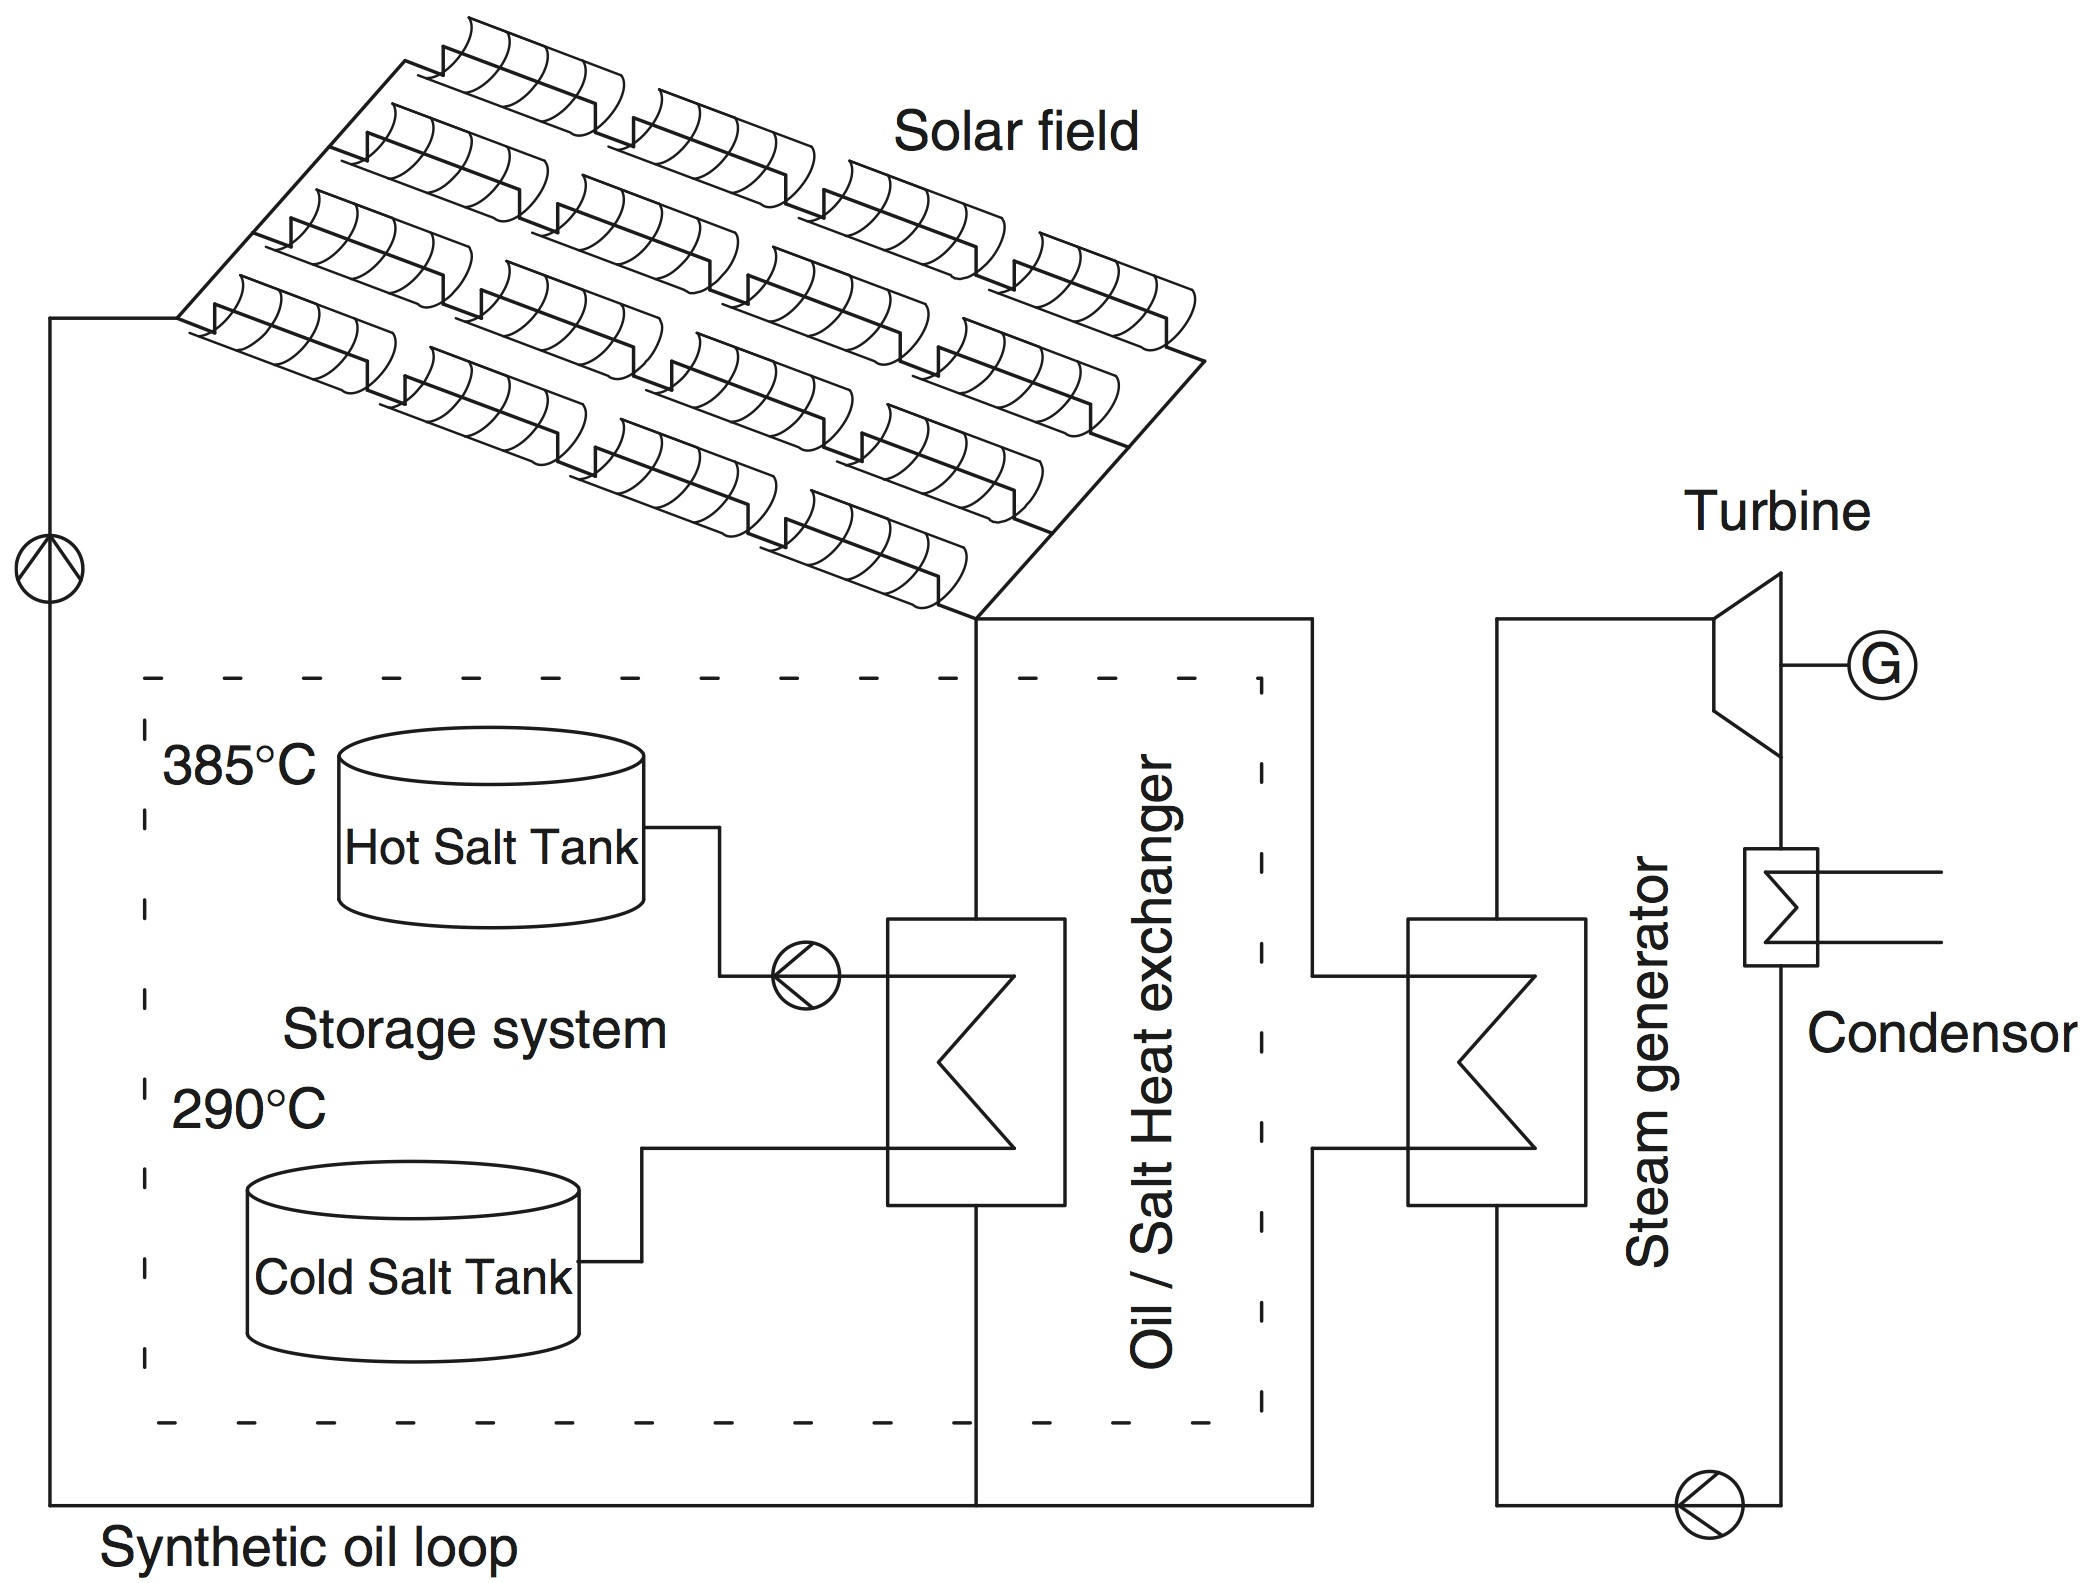
\includegraphics[width=0.65\linewidth]{FIG/troughtindirecttwotank}
\caption[Simplified scheme of PTC power plant with indirect storage system.]{Simplified scheme of PTC power plant with indirect storage system \cite{Steinmann2012}.}\label{troughtindirecttwotank}
\end{figure}
%The parabolic shaped mirrors and the HCE are typically assembled on a support structure mounted on a series of aligned pylons. The center pylon is equipped with a hydraulic drive system to allow tracking of the total solar collector assembly (SCA). Figure~\ref{SCA_EuroTrough} shows a SCA exemplary by using the EuroTrough system. The solar field of a PTC system consists of one or more parallel loops of SCAs. A common header pipe provides each loop with an equal flow rate of HTF. A second header collects the hot HTF to return it either directly to the power cycle or to the TES. \cite{Lupfert2013,Maccari2015}
The parabolic mirrors and the \ac{HCE} are typically assembled on a support structure mounted on a series of aligned pylons. The center pylon is equipped with a hydraulic drive system to allow the complete \ac{SCA} to track the sun. Figure~\ref{SCA_EuroTrough} shows a SCA, the EuroTrough system. The solar field of a PTC system consists of one or more parallel loops of \acp{SCA}. A common header pipe supplies each loop with \ac{HTF} at equal flow rates. A second header collects the hot \ac{HTF} to return it either directly to the power cycle or to the \ac{TES} \cite{Lupfert2013,Maccari2015}.


\begin{figure}[htbp] 
\centering
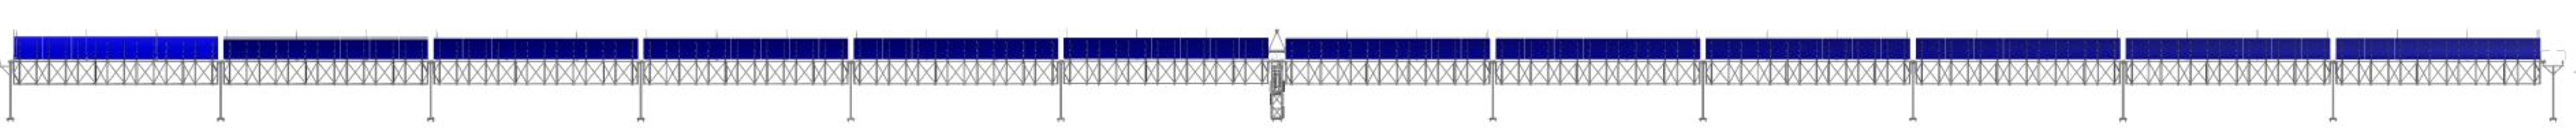
\includegraphics[width=1\linewidth]{FIG/SCA_EuroTrough}
\caption[Typical solar collector assembly composed of 12 EuroTrough collector elements.]{Typical solar collector assembly (SCA) composed of 12 EuroTrough collector elements \cite{VonReeken2014}.}\label{SCA_EuroTrough}
\end{figure}
%Current collector sizes varied from \SIrange{2.55}{8}{\metre}, but in order to reduce the total costs of PTC systems the trend for commercial scaled collector sizes is increasing. \cite{AbengoaSolar2013b,Pitz-Paal.2013,VonReeken2014}
%
%All commercial scale PTC systems uses actually oil based HTF. The first commercial used PTC power plant \emph{SEGS-1}, built 1984 in California, uses a mineral oil as HTF in the HCE, which heats up from \SIrange{240}{305}{\celsius}. The upper temperature end for a stable use of mineral oil is around \SI{300}{\celsius}. In order to increase the maximum process temperature actual PTC systems uses synthetic oil with a maximum working temperature of \SI{400}{\celsius}. \cite{Gil2010,Richter2013,Therminol2015}

Collector sizes vary from \SIrange{2.55}{8}{\metre}, but in order to reduce the total costs of \ac{PTC} systems, the trend is toward collector sizes \cite{AbengoaSolar2013b,Pitz-Paal.2013,VonReeken2014}.

All commercial-scale \ac{PTC} systems use oil-based \ac{HTF}. The first commercial \ac{PTC} power plant, \emph{SEGS-I}, built in 1984 in California, uses a mineral oil as \ac{HTF} in the \ac{HCE}, which reaches temperatures between \SI{240}{\celsius} and \SI{305}{\celsius}. Beyond \SI{300}{\celsius}, mineral oils begin to deteriorate. In order to increase the maximum process temperature, modern \ac{PTC} systems use synthetic oil with a maximum working temperature of \SI{400}{\celsius} \cite{Gil2010,Richter2013,Therminol2015}.

%Synthetic oil is quite expansive therefore it is not used as fluid for TES aplication. Molten salt is more than ten times less expansive, that's the main reason why it is currently used as storage medium in the TES of PTC systems \cite{Gil2010}. 
%
%There is a huge research and development expenses for using molten salt also as HTF in the HCE for PTC systems, but currently there are no commercial scale PTC power plants projects with molten salt applications as HTF known. \cite{Maccari2015}

Synthetic oil is not employed in \ac{TES} applications owing to its expense. Molten salt is one-tenth the cost \cite{Gil2010}. Though considerable effort and expense are being devoted to research into molten salt as \ac{HTF} for \ac{PTC} systems, there are currently no commercial-scale \ac{PTC} power plant projects \cite{Maccari2015}.

%At this stage it can be noted, that PTC uses a lower thermal process temperature than the CR systems, which effects on the one hand the efficiency of the thermal process (Rankine cycle) and on the other hand the required dimensions of the TES medium. 
%
%Furthermore must be noted that the power output of a PTC plant is more effected by the seaseonal variation of the irradiance angle due to not traking the sun in two axis and a thereby resulting higher cosine efficinetcy loss. \cite{Jorgenson2013}

\ac{PTC} systems have a lower thermal process temperature than \ac{CR} systems, which impacts the efficiency of the thermal process (Rankine cycle) and influences the required dimensions of the \ac{TES} medium. The output of a \ac{PTC} plant is more strongly influenced by the seasonal variation of the irradiance angle, as it tracks the sun in one axis only and suffers from higher cosine efficiency loss as a result \cite{Jorgenson2013}.

\section{Large-scale PV power plants}\label{Large scale photo voltaic (PV) power plants}
%PV cells are semiconductor devices that convert solar irradiance due to the photovoltaic effect directly into direct current (DC).
%Grid-tied systems require inverters to transform DC power in alternating current (AC). Therefore it is in the nature of PV systems that the generate power just during daytime. To support the South African system load even at the most critical time - the evening hours - the PV system needs a storage opportunity for electrical power. Such an electrical energy storage (EES) could either be DC- or AC-site connected with the PV system depending on the EES technology. Figure~\ref{PVMainComp} shows a with a EES extended feasible PV plant scheme.

Photovoltaic cells are semiconductor devices that convert solar irradiance directly into \ac{DC} via the photovoltaic effect.
Grid-tied systems require inverters to transform \ac{DC} into \ac{AC}. To support the South African system load even at the most critical time - the evening hours - the PV system must be complemented by storage. Such electrical energy storage \ac{EES} can either be \ac{DC}- or \ac{AC}-site connected with the PV system, depending on the \ac{EES} technology. Figure~\ref{PVMainComp} shows an \ac{EES}-extended feasible \ac{PV} plant scheme.


\begin{figure}[!h] 
\centering
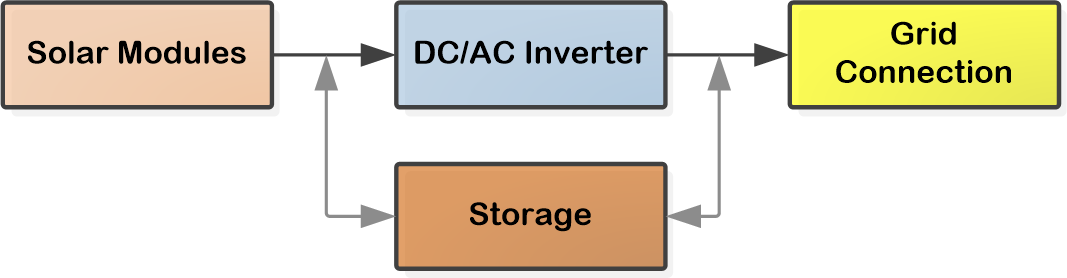
\includegraphics[width=0.8\linewidth]{FIG/PVMainComp}
\caption[Main components of feasible a PV plant.]{Main components of feasible a PV plant.}\label{PVMainComp}
\end{figure}
Such a \ac{PV} plant scheme is currently not in a commercial use and is therefore more of theoretically nature. Nevertheless with this schema the covering of the prescribed load curve is conceivable.
\subsubsection{Large-scale PV systems}
%As it was said above, PC cells generates electricity in form of DC power. The cells are interconnected to form modules, which are then combined to form arrays and systems. PV can be used in various applications with capacities from less then one watt up to hundreds of megawatts. The balance of system (BOS) of grid-tied PV systems includes inverters, transformer, wiring and monitoring equipment, as well as structural components for installing modules.  
\ac{PV} cells are interconnected to form modules, which are then combined to form arrays and systems. \ac{PV} may be used in applications with capacities under one watt up to hundreds of megawatts. The \ac{BOS} of grid-tied \ac{PV} systems includes inverters, transformer, wiring and monitoring equipment, as well as structural components for installing modules.  

%Crystalline silicon (c-Si) modules, whether single- (sc-Si also known as mono-Si) or multi-crystalline (mc-Si also known as multi-Si), largely dominate the PV-market. Cells are usually sliced from ingots or castings of highly purified silicon. The manufacturing process creates a potential junction, deposits an anti-reflective costing and adds metal contacts. Cells are then grouped into modules with a transparent glass for the front, a weatherproof material for the back and often a rounded by a frame. Modules are usually guaranteed for a lifetime of 20 years at minimum \SI{80}{\percent} of there rated output, and sometimes at \SI{70}{\percent} for 30 years. In the last 10 years, the efficiency of average commercial silicon modules increased from about \SIrange{12}{16}{\percent}, while the record lavatory cell efficiency is currently \SI{25.6}{\percent} for sc-Si and \SI{20.8}{\percent} for mc-Si wafer-based technology. \cite{FraunhoferISE2015}
Crystalline silicon (c-Si) modules, whether single- (sc-Si also known as mono-Si) or multi-crystalline (mc-Si also known as multi-Si), dominate the PV-market. Cells are usually sliced from ingots or castings of highly purified silicon. The manufacturing process creates a potential junction, deposits an anti-reflective coating and adds metal contacts. Cells are then grouped into modules with a transparent glass in the front, a weatherproof material in the back and often enclosed by a frame. Modules are typically guaranteed for a lifetime of 20 years at a minimum \SI{80}{\percent} of rated output, and occasionally at \SI{70}{\percent} for 30 years. In the last 10 years, the efficiency of average commercial silicon modules has increased from \SI{12}{\percent} to \SI{16}{\percent}, while the record laboratory cell efficiency is currently \SI{25.6}{\percent} for sc-Si and \SI{20.8}{\percent} for mc-Si wafer-based technology. \cite{FraunhoferISE2015}

%Two main alternative solar cell commercial technologies exist: multi-junction cells, used in CPV (will not be dealt with any further) and thin films, based on either amorphous silicon (a-Si), cadmium-telluride (CdTe), copper-indium-(di)selenide (CIS), copper-indium-gallium-(di)selenide (CIGS) or copper-zinc-tin-sulfide \cite{IEA2014c}. The highest lab efficiency in thin film technology is \SI{21.0}{\percent} for CdTe and \SI{20.5}{\percent} for CIGS solar cells. The efficiency of average commercial CdTe module increased from \SIrange{9}{13}{\percent} in the last 10 years \cite{FraunhoferISE2015}.

Two commercially viable alternative \ac{PV} technologies exist: multi-junction cells, used in \ac{CPV} (which will not be addressed here) and thin films, based on either amorphous silicon (a-Si), cadmium-telluride (CdTe), copper-indium-(di)selenide (CIS), copper-indium-gallium-(di)selenide (CIGS) or copper-zinc-tin-sulfide \cite{IEA2014c}. The highest laboratory efficiency in thin film technology is \SI{21.0}{\percent} for CdTe and \SI{20.5}{\percent} for CIGS solar cells. The efficiency of average commercial CdTe modules increased from \SI{9}{\percent} to \SI{13}{\percent} in the last 10 years \cite{FraunhoferISE2015}.

%PV is a fast growing market as it can be seen in Figure~\ref{PV_Prod_by_Tech}. A global installing rate of about \SI{130}{\mega\watt} new PV systems per day should therefore be expected for 2014. The Compound Annual Growth Rate (CAGR) of PV installations was \SI{44}{\percent} between 2000 to 2014 \cite{FraunhoferISE2015}. 

The \ac{PV} market has grown rapidly (Figure~\ref{PV_Prod_by_Tech}). An expansion rate of \SI{130}{\mega\watt\per\day} is expected for 2014. The Compound Annual Growth Rate (CAGR) of \ac{PV} installations was \SI{44}{\percent} between 2000 and 2014 \cite{FraunhoferISE2015}. 


\begin{figure}[htbp]  
\centering
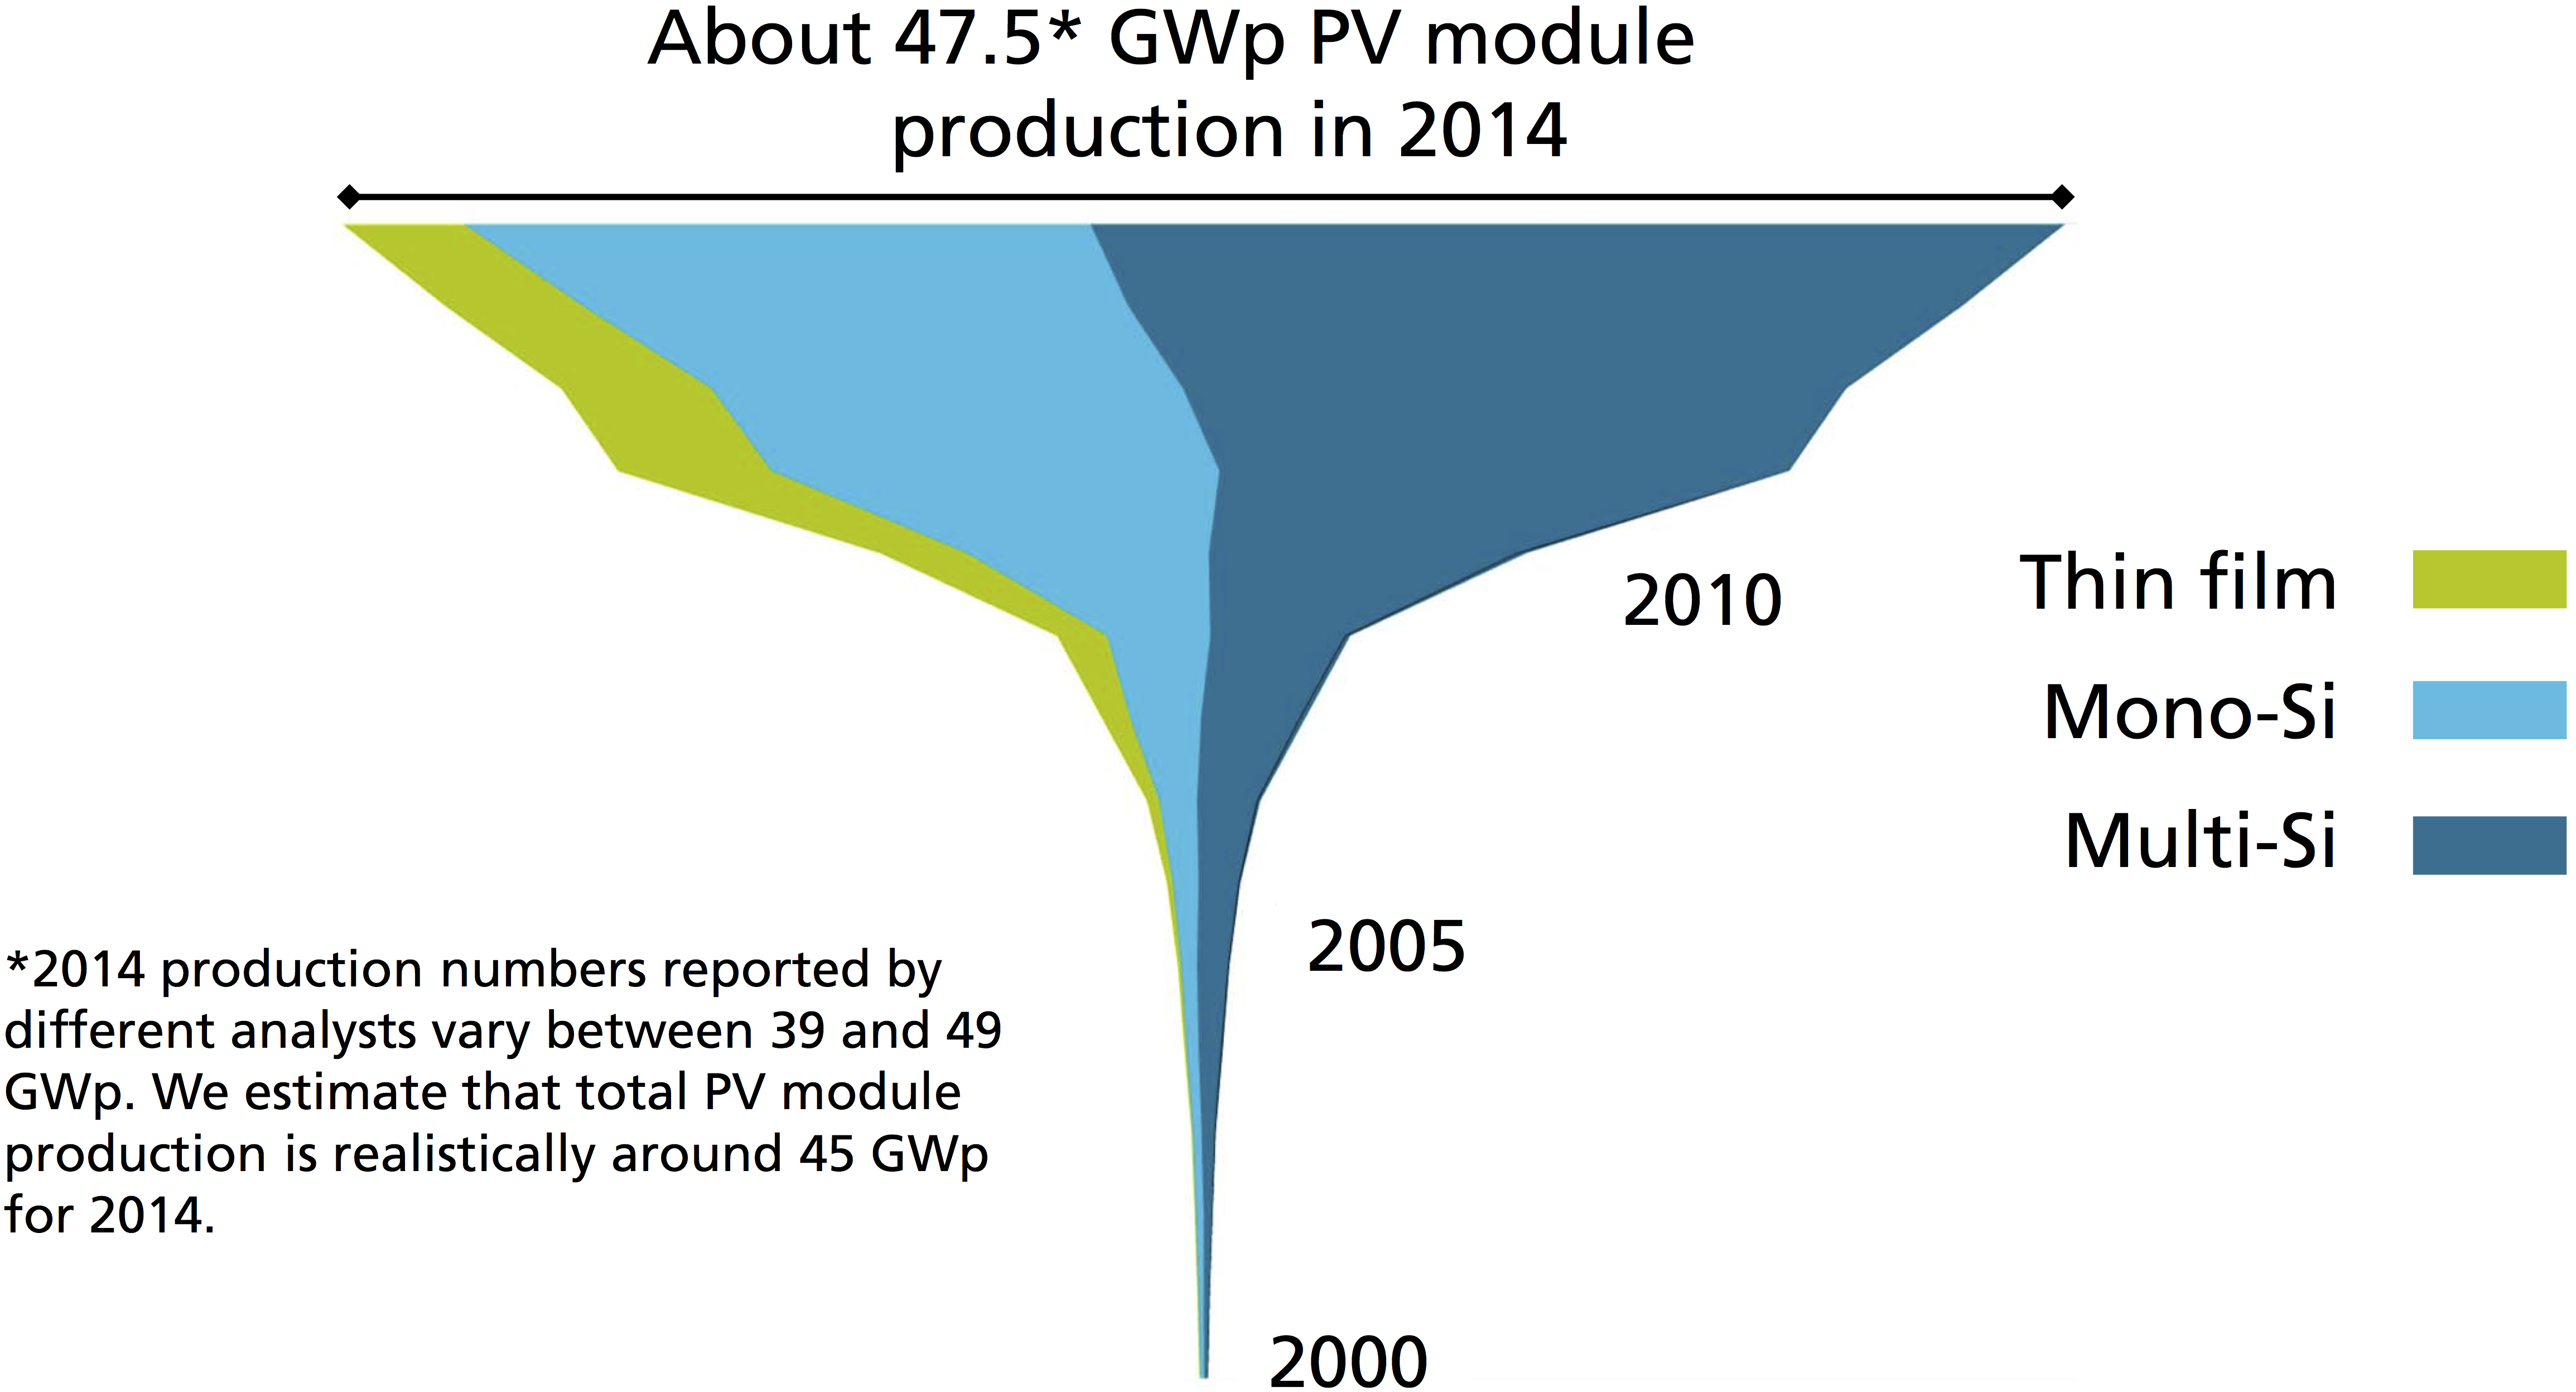
\includegraphics[width=0.7\linewidth]{FIG/PV_Prod_by_Tech}
\caption[Worldwide annual PV production by technology.]{Worldwide annual PV production by technology in \si{\giga\watt}\textsubscript{p} \cite{FraunhoferISE2015}.}\label{PV_Prod_by_Tech}
\end{figure}
%Since 2010 the world has added more PV capacity than it had in the previous four decades \cite{IEA2014c}. In 2014 the worldwide installed cumulative PV capacity was about \SI{183}{\giga\watt}\textsubscript{p} whereof \SI{21}{\percent} are allocated Germany. About \SI{80}{\percent} of the actually worldwide cumulative installed PV capacity is assigned to Europe and Asia. Figure~\ref{PV_Install_global} shows the development of the worldwide cumulative installed PV capacity from 2008 to 2014. \cite{FraunhoferISE2015}

Since 2010, the world has added more \ac{PV} capacity than it had in the previous four decades \cite{IEA2014c}. In 2014, the worldwide installed cumulative \ac{PV} capacity was about \SI{183}{\giga\wattp}, of which \SI{21}{\percent} is in Germany. About \SI{80}{\percent} of the current worldwide cumulative installed \ac{PV} capacity is found in Europe and Asia. Figure~\ref{PV_Install_global} shows the development of the worldwide cumulative installed \ac{PV} capacity from 2008 to 2014 \cite{FraunhoferISE2015}.


\begin{figure}[htbp]  
\centering
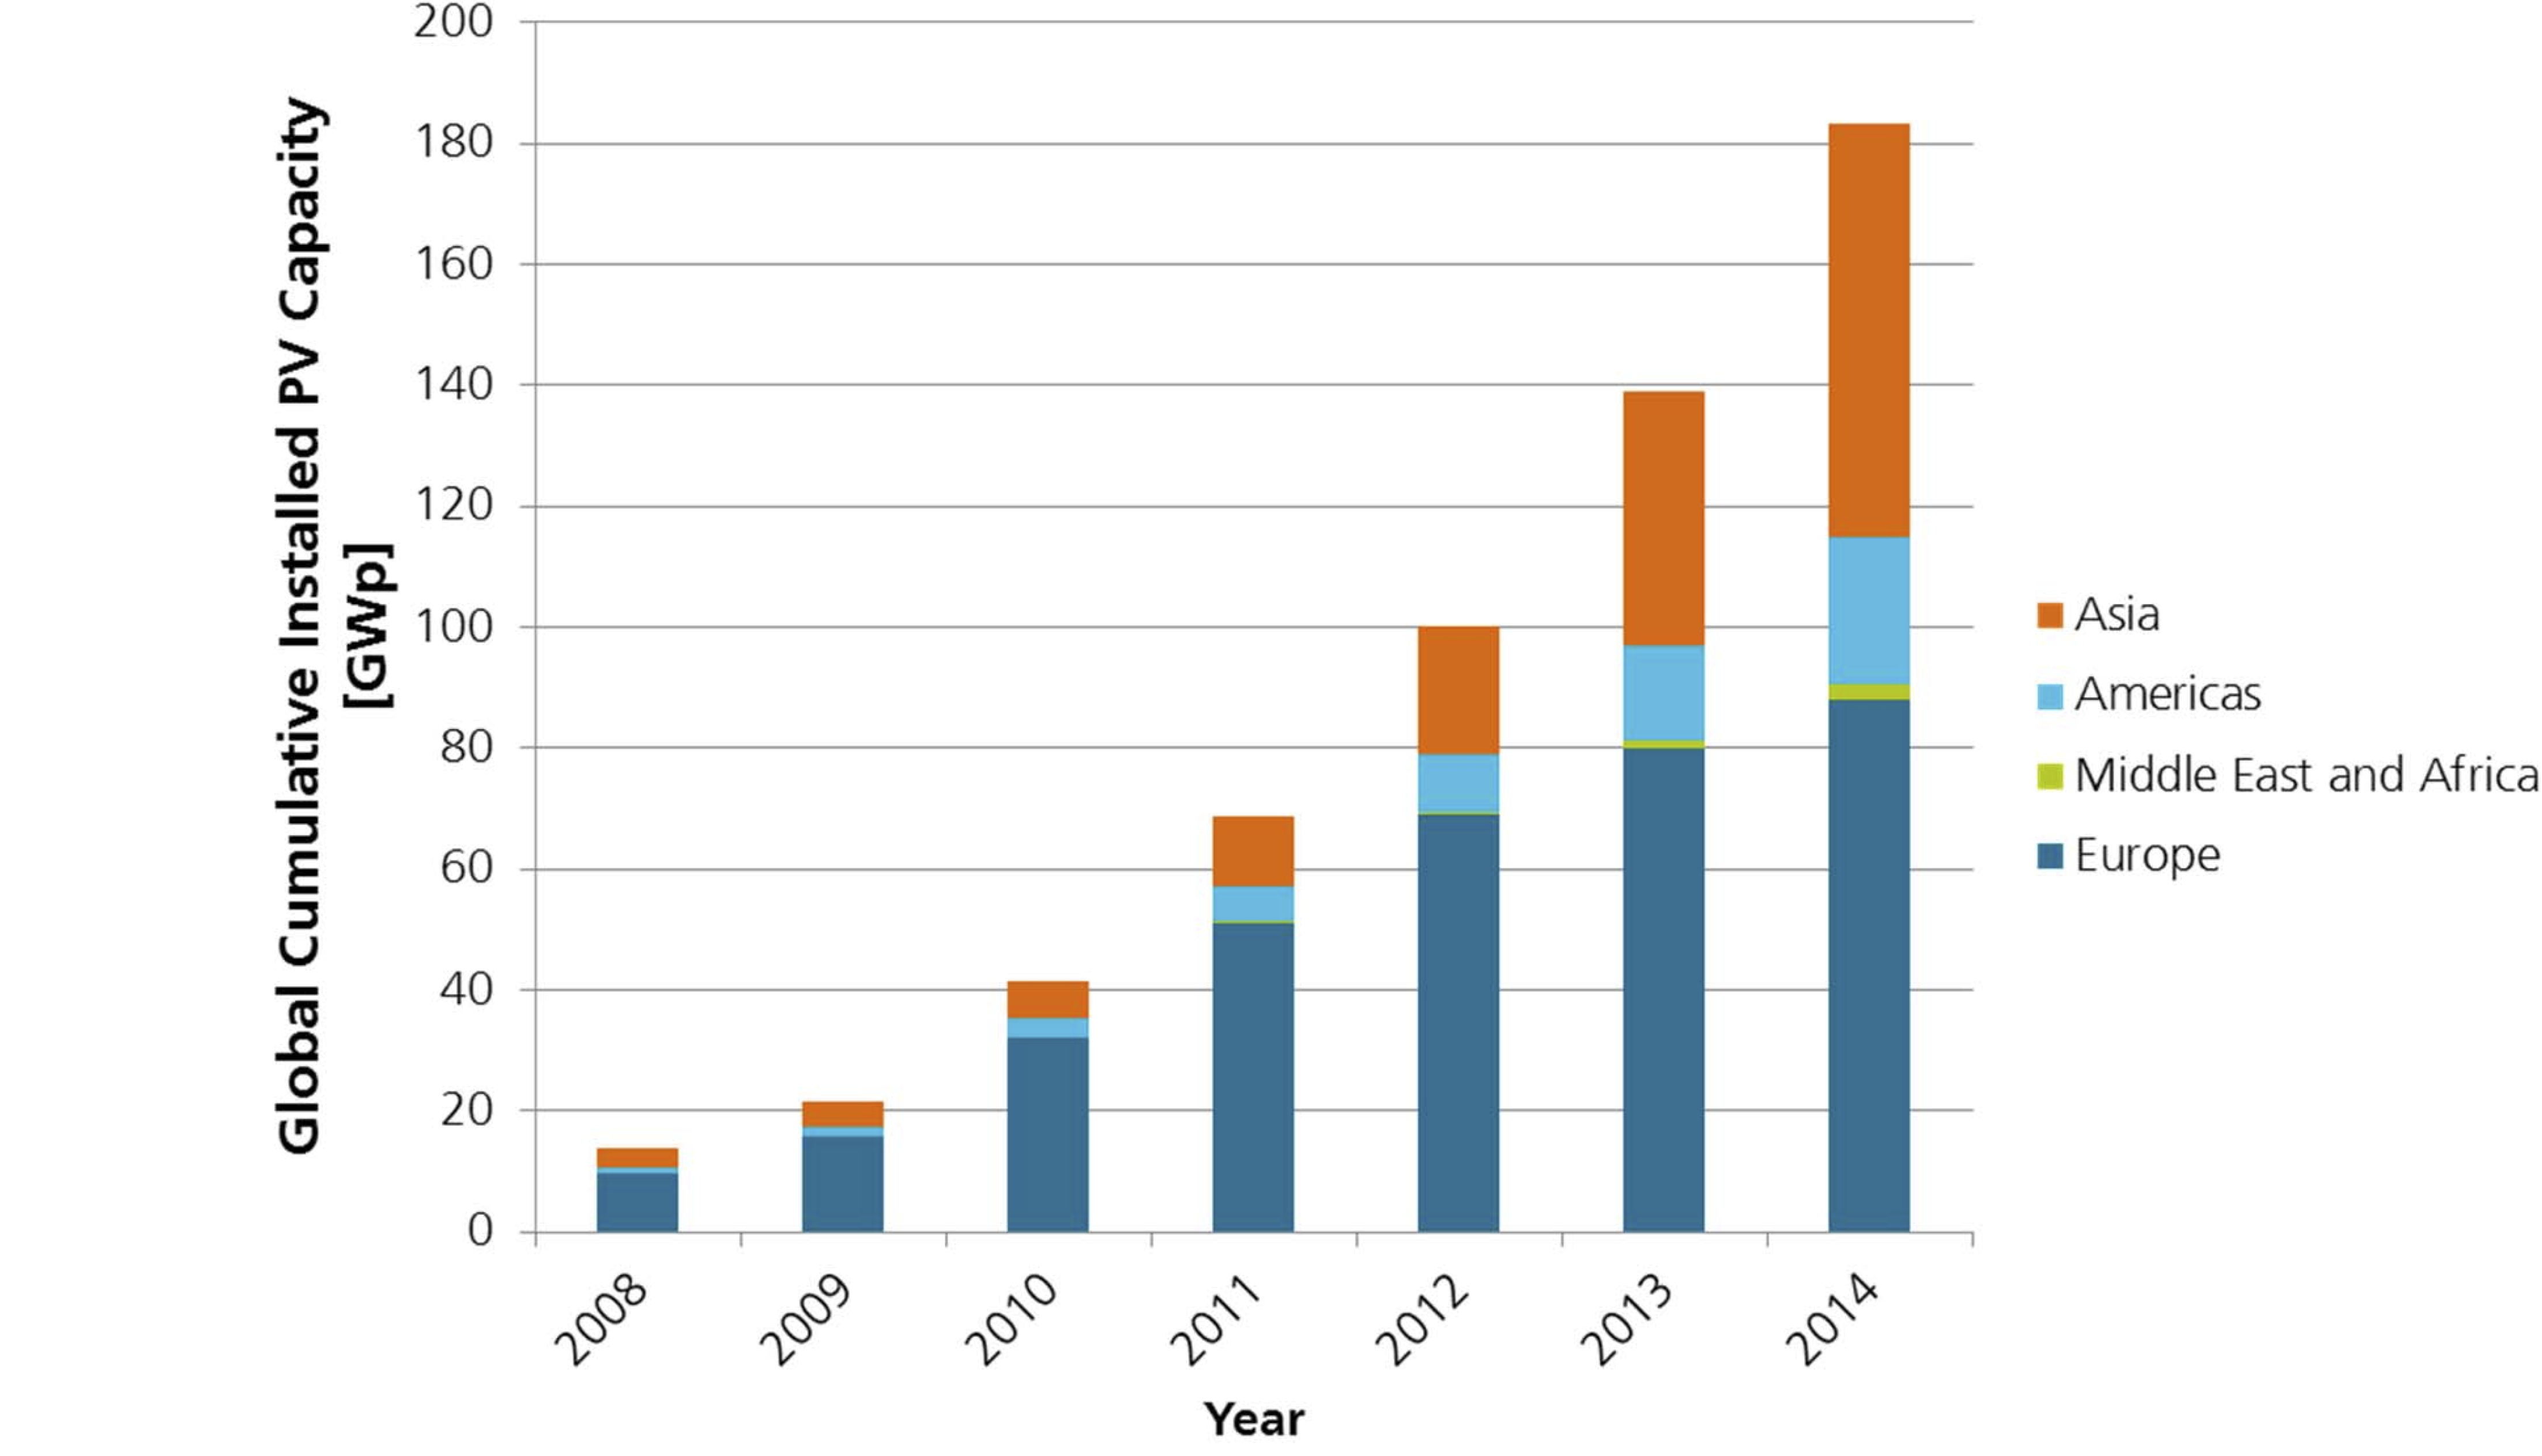
\includegraphics[width=0.7\linewidth]{FIG/PV_Install_global}
\caption[Worldwide cumulative PV installation until 2014.]{Worldwide cumulative PV installation until 2014 \cite{FraunhoferISE2015}.}\label{PV_Install_global}
\end{figure}
%The emergence of the global PV market has stimulated rapid cost reductions of modules and systems. In the last few years, intense competition and global over capacities led many PV cell and module manufacturer to price their products too low for investment cost recovery, and thereby several companies failed. 
The emergence of a global \ac{PV} market has driven rapid cost reductions of modules and systems. In the last few years, intense competition and global over-capacities forced many manufacturers to price their products below cost, resulting in bankruptcies and consolidations. 

%In 2013 PV systems cost about \SIrange{30}{44}{\percent} what they cost in 2008 (see Figure~\ref{PVsystemCosts}). Prices for PV systems are more diversified than for cells and modules, which tend to be global commodities. Small systems, such as rooftop, are more expansive than larger ones, especially ground-based, unity-scale systems. The prices for the different system types varies significantly among countries. Most of the gap comes from differences in "soft costs", which includes permitting, inspection, interconnection and labour costs \cite{IEA2014c}. Therefore it is important to use country-specific prices for calculating costs.
In 2013, \ac{PV} systems cost \SIrange{30}{44}{\percent} what they cost in 2008 (see Figure~\ref{PVsystemCosts}). Prices for complete \ac{PV} systems are more heterogenous than for cells and modules, which are increasingly commodity products. Small rooftop systems are more expensive per \si{\wattp} than larger ones, especially ground-based, unity-scale systems. Costs vary significantly between countries. Most of the gap comes from differences in "soft costs", which includes permitting, inspection, interconnection and labour costs \cite{IEA2014c}, so it is important to obtain country-specific costs when calculating budgets.

\begin{figure}[htbp]  
\centering
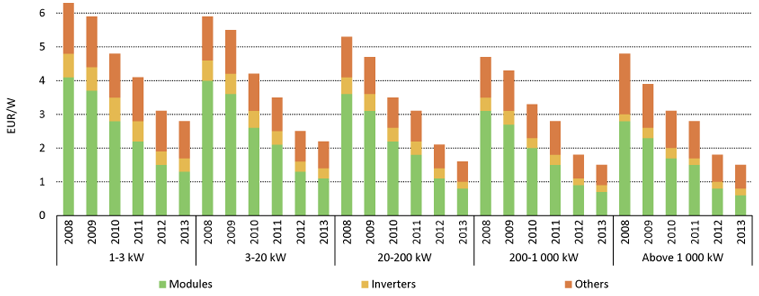
\includegraphics[width=1\linewidth]{FIG/PVsystemCosts}
\caption[PV system cost development by size.]{PV system cost development in Italy by size \cite{IEA2014c}.}\label{PVsystemCosts}
\end{figure}
%Installations for unity-scale PV systems in SA currently has a similar cost distribiution then it is shown actually in Itally. Modules makes in SA a share of \SI{37}{\percent} of the total investment cost, while it is \SI{40}{\percent} in Italy. The share of Inverter costs makes \SI{10}{\percent} in SA and \SI{13}{\percent} in Itally. Therefore it can be noteced that the share of further soft costs is higher for unity-scale PV systems in SA then in Italy and makes more than the half of installation costs. \cite{IEA2014c,Terblanche2015}
Unity-scale \ac{PV} systems in South Africa have a similar cost structure to that typical for Italy (Figure \ref{PVsystemCosts}). Modules make up \SI{37}{\percent} of the total investment cost, versus \SI{40}{\percent} in Italy. The inverter share is \SI{10}{\percent} in South Africa and \SI{13}{\percent} in Italy. Soft costs are significantly higher for unity-scale \ac{PV} systems in South Africa, accounting for more than half of installation costs \cite{IEA2014c,Terblanche2015}.

\subsubsection{Large-scale electrical energy storage systems}
%For supplying the in Section~\ref{SystemloadinSA} prescribed load curve even due to night time the PV system needs assistance by a EES. In generally can be said that a EES consists by two main sections, namely the power conversion system (PCS) and the energy storage unit. A PCS is used to adjust the voltage, current, and other power characteristics of the storage based on the load requirements. PCS may consist of two separated units for charging and discharging with different characteristics. Energy storage section is the other part of EES that is designated to contain the storage medium, e.g. water reservoirs in pumped hydroelectric storage (PHS). Because PCS and energy storage units have inherent inefficiencies and losses, overall efficiency of EES technologies is defined by Equation~\ref{Overall storage efficiency}, in which $E_{out}$ and $E_{in}$ are output and input electric energy, respectively \cite{Kaldellis2009}.
To meet the prescribed load curve even in darkness, the \ac{PV} system must have \ac{EES}. Electrical energy storage consists of the \ac{PCS} and the energy storage unit. A \ac{PCS} is used to adjust the voltage, current, and other power characteristics of the storage based on the load requirements. Power conversion systems may consist of two separated units for charging and discharging with different characteristics. The energy storage section is that part of the \ac{EES} that contains the storage medium, \emph{e.g.} water reservoirs in \ac{PHS}. Because \ac{PCS} and energy storage units have inherent inefficiencies and losses, the overall efficiency of \ac{EES} technologies is defined by Equation~\ref{Overall storage efficiency}, in which $E_{out}$ and $E_{in}$ are output and input electric energy, respectively \cite{Kaldellis2009}.

\begin{equation}
\textrm{Overall storage efficiency}=\frac{E_{out}}{E_{in}} \label{Overall storage efficiency}
\end{equation}
Figure~\ref{TCC_EES} illustrates the main sections of a typical \ac{EES} system and the associated losses.

\begin{figure}[htbp]  
\centering
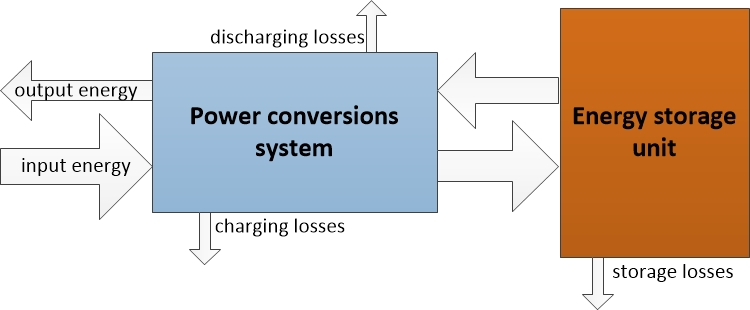
\includegraphics[width=0.65\linewidth]{FIG/EESSchema}
\caption[Main sections of electrical energy storage system and there energy losses.]{Main sections of electrical energy storage (EES) system and there energy losses.}\label{TCC_EES}
\end{figure}
%In 2014 the global large-scale energy storage capacity was more than \SI{140}{\giga\watt} of which about \SI{97}{\percent} was allocated by PHS. Rapid deployment of wind and solar PV energy has led to integrate challenges and the need for more flexible storage opportunities. Thereby also alternative grid connected energy storage concepts are growing. Between 2005 and 2014 there was a sharp increase in global capacity of large-scale battery storages from \SIrange{120}{690}{\mega\watt}. Figure~\ref{EESgridCapacity} describes the global capacity development for grid connected storage. It must be noted, that the thermal storage share in this chart also includes decentralized hot water boilers, which is not to be confused with TES of CSP applications.
In 2014, the global large-scale energy storage capacity was more than \SI{140}{\giga\watt}, of which \SI{97}{\percent} was \ac{PHS}. Rapid deployment of wind and solar \ac{PV} energy has led to integration challenges and the need for more flexible storage. Between 2005 and 2014, there was a sharp increase in installed large-scale battery storage from \SI{120}{\mega\watt} to \SI{690}{\mega\watt} Figure~\ref{EESgridCapacity}.


\begin{figure}[htbp]  
\centering
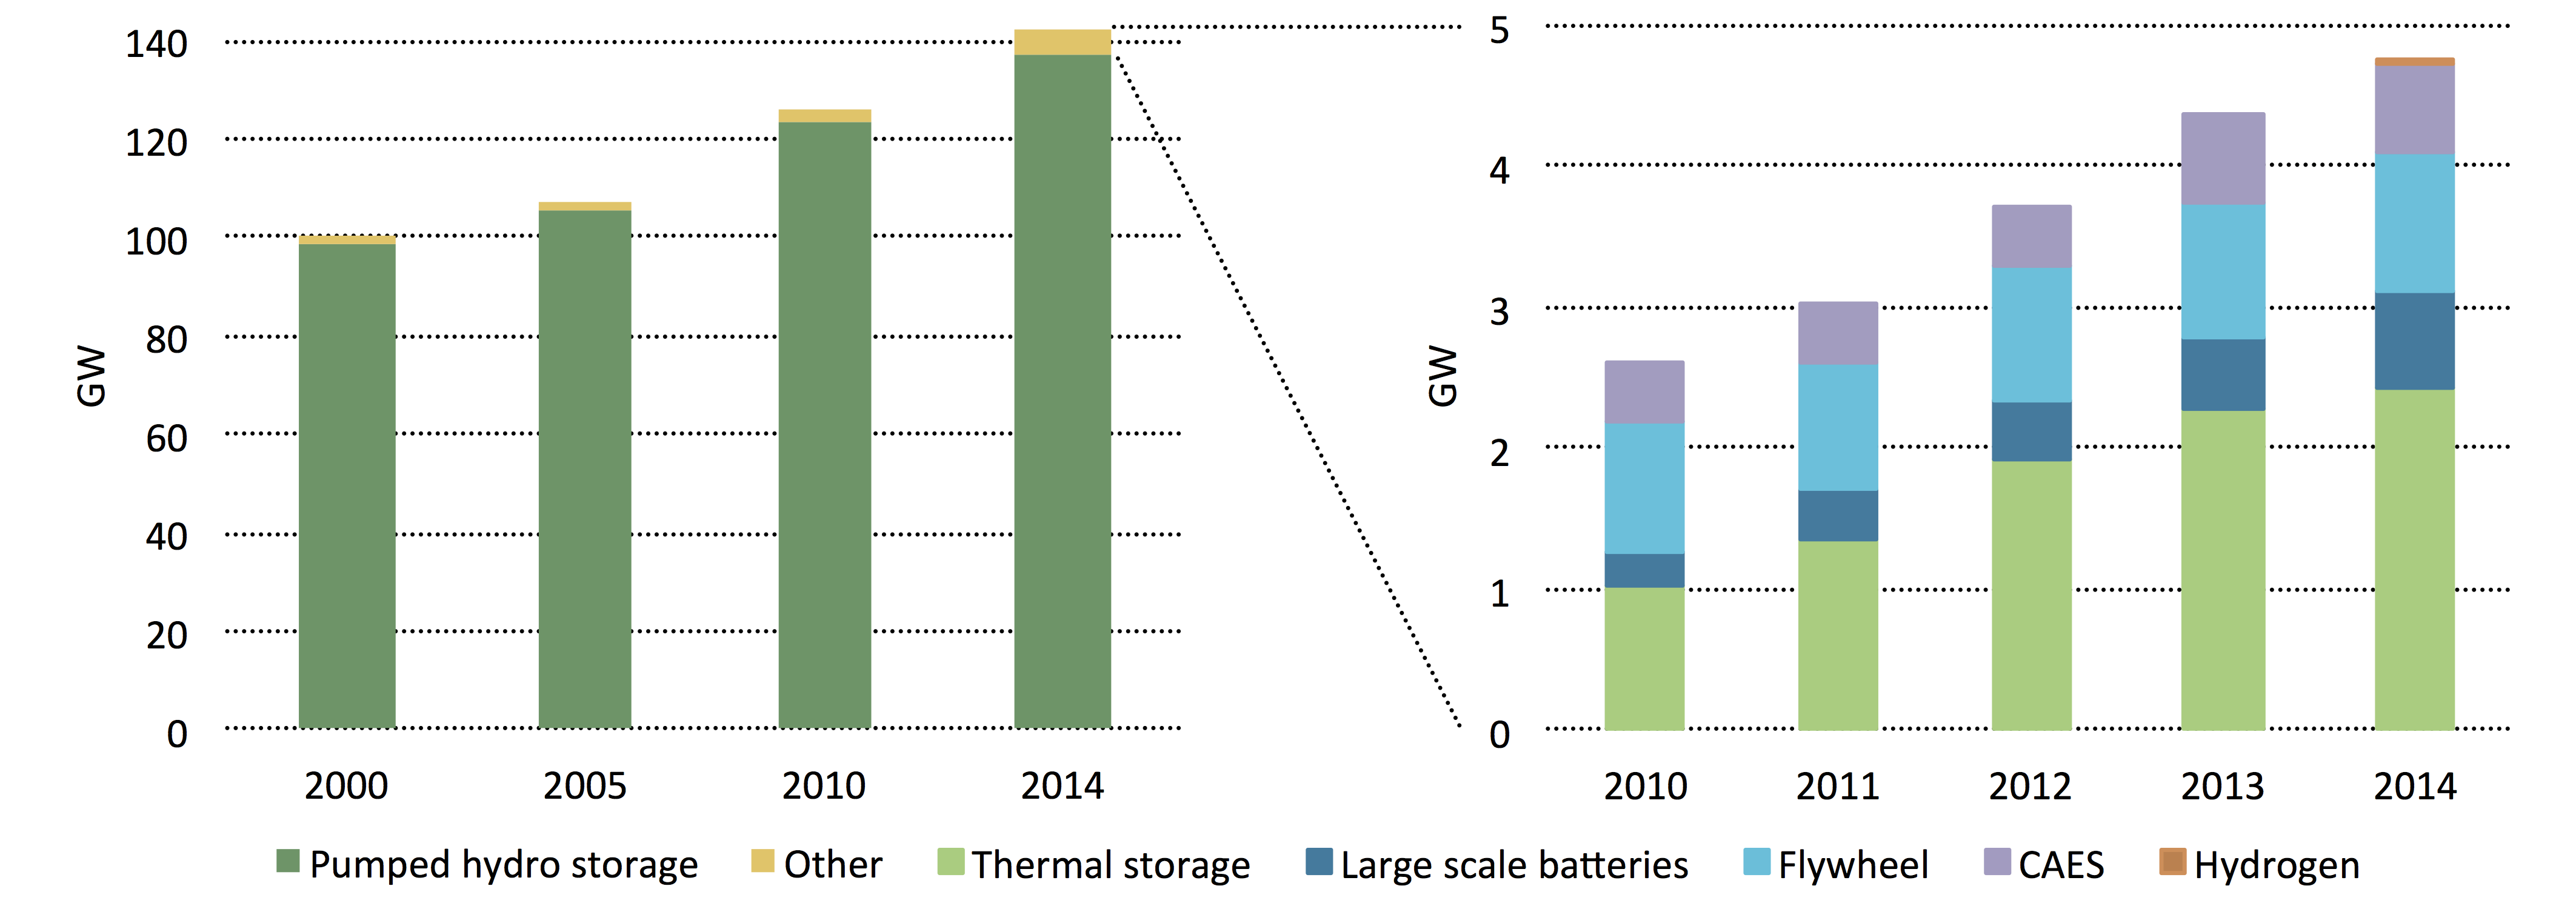
\includegraphics[width=1\linewidth]{FIG/EESgridCapacity}
\caption[Worldwide installed capacity for grid connected storage.]{Worldwide installed capacity for grid connected storage \cite{IEA2015}.\footnote{Thermal storage share includes decentralized hot water boilers, which are not to be confused with TES in CSP applications.}}\label{EESgridCapacity}
\end{figure}

%For supporting the PV system by supplying the prescribed load curve, the EES requires a Power output of about \SI{100}{\mega\watt} and a storage capacity from several hours. Therefor not many technologies comes into question. Figure~\ref{EEStechnologies} shows that just four EES technology fields could meet the requirements of the prescribed load, namely pumped hydroelectric storage (PHS), compressed air energy storage (CAES), hydrogen (H\textsubscript{2}) storage and battery storage.
To match the prescribed load curve, the \ac{EES} requires a power output of \SI{100}{\mega\watt} and several hours of storage capacity. Of the available \ac{EES} technologies, four meet the requirements of the prescribed load, namely \acf{PHS}, \acf{CAES}, hydrogen (H\textsubscript{2}) storage and battery storage (Figure~\ref{EEStechnologies}).

%The PHS technology is fully mature and reaches efficiency ranges of \SIrange{70}{85}{\percent} with lifetimes between 20~000 and 50~000 cycles \cite{IEA2014c}. But the applicability of this technology is required by potential energy of the storage medium and is therefore highly limited by the regional landscape and there differences in altitude. Furthermore is the apply of PHS in desert regions not well located due to high evaporation losses.

\ac{PHS} technology is fully mature and reaches efficiency ranges of \SIrange{70}{85}{\percent} with lifetimes between 20~000 and 50~000 cycles \cite{IEA2014c}. But the applicability of this technology is a function of the potential energy of the storage medium and is therefore limited by the landscape and differences in altitude. Desert regions make poor sites for \ac{PHS} due to high evaporation losses.

%The overall storage efficiency of the H\textsubscript{2} storage is below \SI{40}{\percent} and mainly still in demonstration stage \cite{IEA2014c,IEA2015}. Therefore this technology is also not suited for a adaption to a PV system.
The overall storage efficiency of H\textsubscript{2} storage is below \SI{40}{\percent}. This technology remains in demonstration \cite{IEA2014c,IEA2015}.

\begin{figure}[htbp]  
\centering
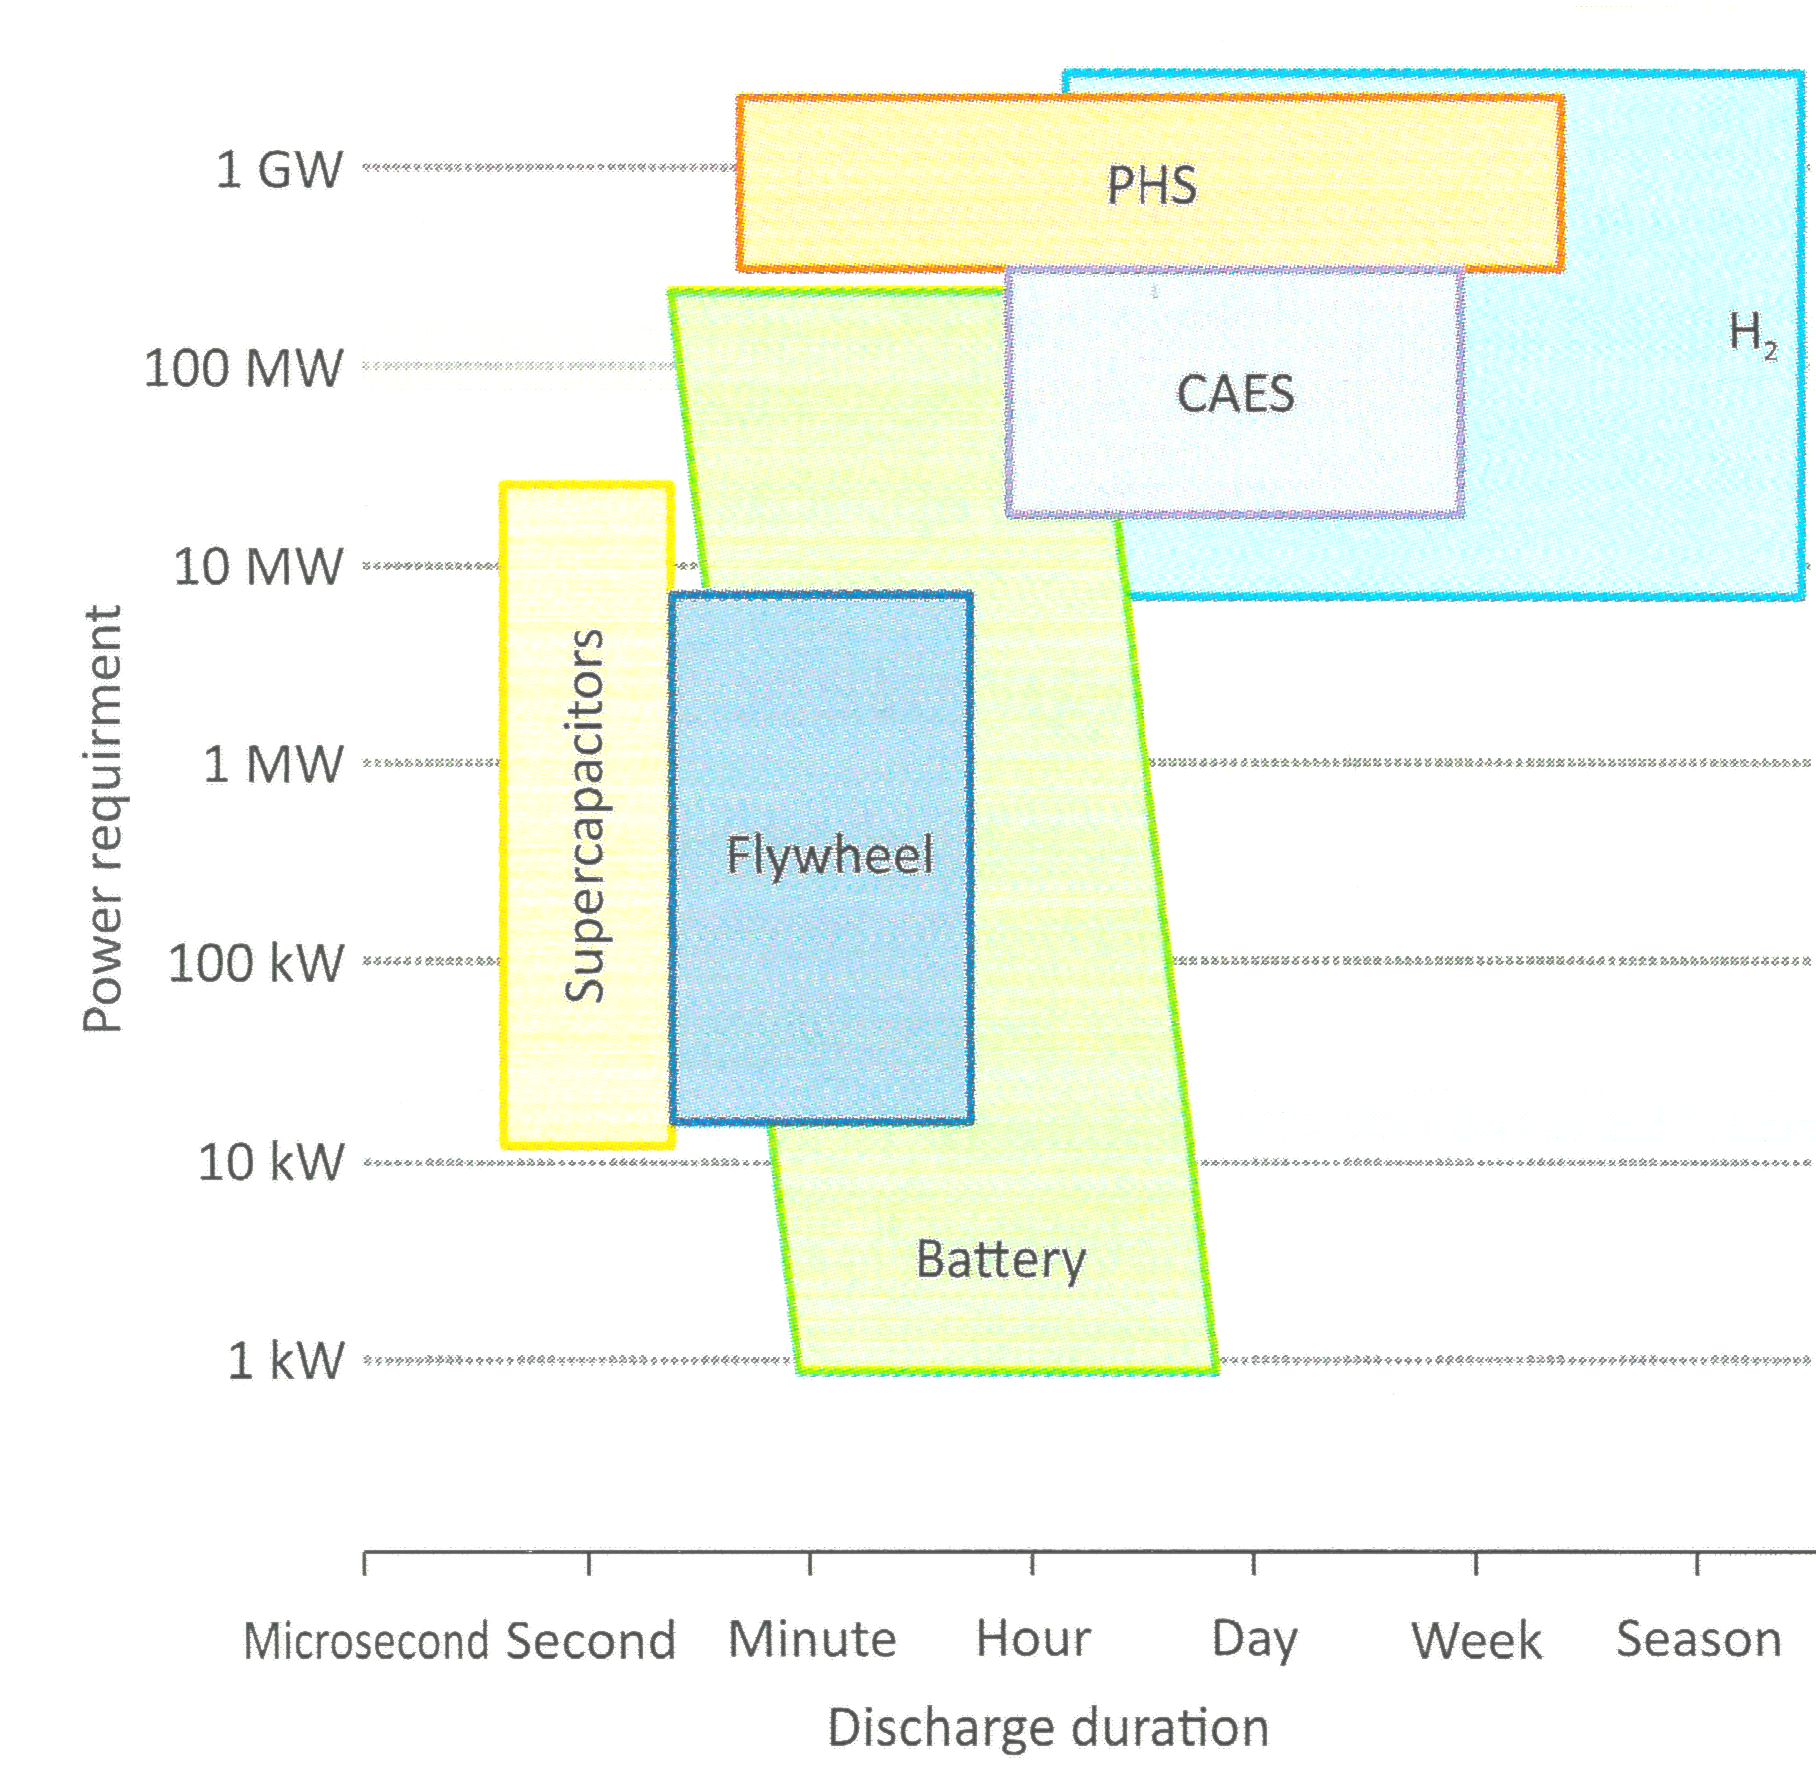
\includegraphics[width=0.6\linewidth]{FIG/EEStechnologies}
\caption[Energy storage technologies ranges.]{Energy storage technologies ranges \cite{IEA2014c}.}\label{EEStechnologies}
\end{figure}
%The CAES technology is at a deployed maturity stage and has a for the application as PV system adapted EES a suitable capacity range of \SIrange{100}{300}{\mega\watt}. Also the cycle lifetime of 10~000 to 25~000 cycles is convincing. But with a range of \SIrange{50}{75}{\percent} efficiency, it would have had to high losses, which must be compensated by a oversized PV system. Thererfor is CAES not applyed in the subsequently comparision.  \cite{IEA2014c}

The \ac{CAES} technology is mature and has a capacity range of \SIrange{100}{300}{\mega\watt} in \ac{PV} applications, as well as an attractive life expectancy of 10~000 to 25~000 cycles. The efficiency range of \SIrange{50}{75}{\percent} mean significant losses which must be compensated by an oversized PV system \cite{IEA2014c}. This makes \ac{CAES} a poor candidate and so it was not used in this analysis.

%Battery storage technology includes different battery technology types, which also distinguish there own individual specifications by fabrication disparities. Most worth mentioning are Lithium-ion (Li-ion) battery with a overall efficiency of \SIrange{85}{95}{\percent} and a lifetime of 1~500 to 10~000 cycles, sodium–sulfur (NaS) battery which has a efficiency range of \SIrange{75}{90}{\percent} at 2~000 to 5~000 cycles, vanadium redox flow battery (VRB or also called VRFB) at a overall efficiency of \SIrange{65}{85}{\percent} and a lifetime of more than 10~000 cycles and lead–acid (LA) battery usally has a overall efficiency of \SIrange{65}{85}{\percent} at a lifetime of 2~000 to 10~000 cycles. \cite{IEA2014c,Zakeri2015}

Battery storage technology includes different battery technology types, which can be differentiated by fabrication method. Most worth mentioning are \ac{li-ion}, with an overall efficiency of \SIrange{85}{95}{\percent} and a lifetime of \num{1500} to \num{10000} cycles, sodium–sulfur (NaS), which has a efficiency range of \SIrange{75}{90}{\percent} at \num{2000} to \num{5000} cycles, vanadium redox flow batteries (VRB or also called VRFB) at an overall efficiency of \SIrange{65}{85}{\percent} and a lifetime of more than \num{10000} cycles, and lead–acid (LA), with an overall efficiency of \SIrange{65}{85}{\percent} a lifetime of \num{2000} to \num{10000} cycles \cite{IEA2014c,Zakeri2015}. Overall, battery storage can be suitable for a \ac{PV} system, though battery life is affected by charge and discharge handling and can vary significantly as a result.

%It can be seen that a battery storage is a suitable solution for adaption to a PV system. But it must be noted, that the cycle lifetime of all batteries is highly effected by the charging and discharging settings and can thereby vary a lot.

%The spread of total capital costs of the different EES technologies can be seen in Figure~\ref{TCC_EES}. It is striking that the range of costs can be huge and highly depends on the specification of the application.

Costs vary widely and depend on the specifics of the application (Figure~\ref{TCC_EES}).


\begin{figure}[htbp]  
\centering
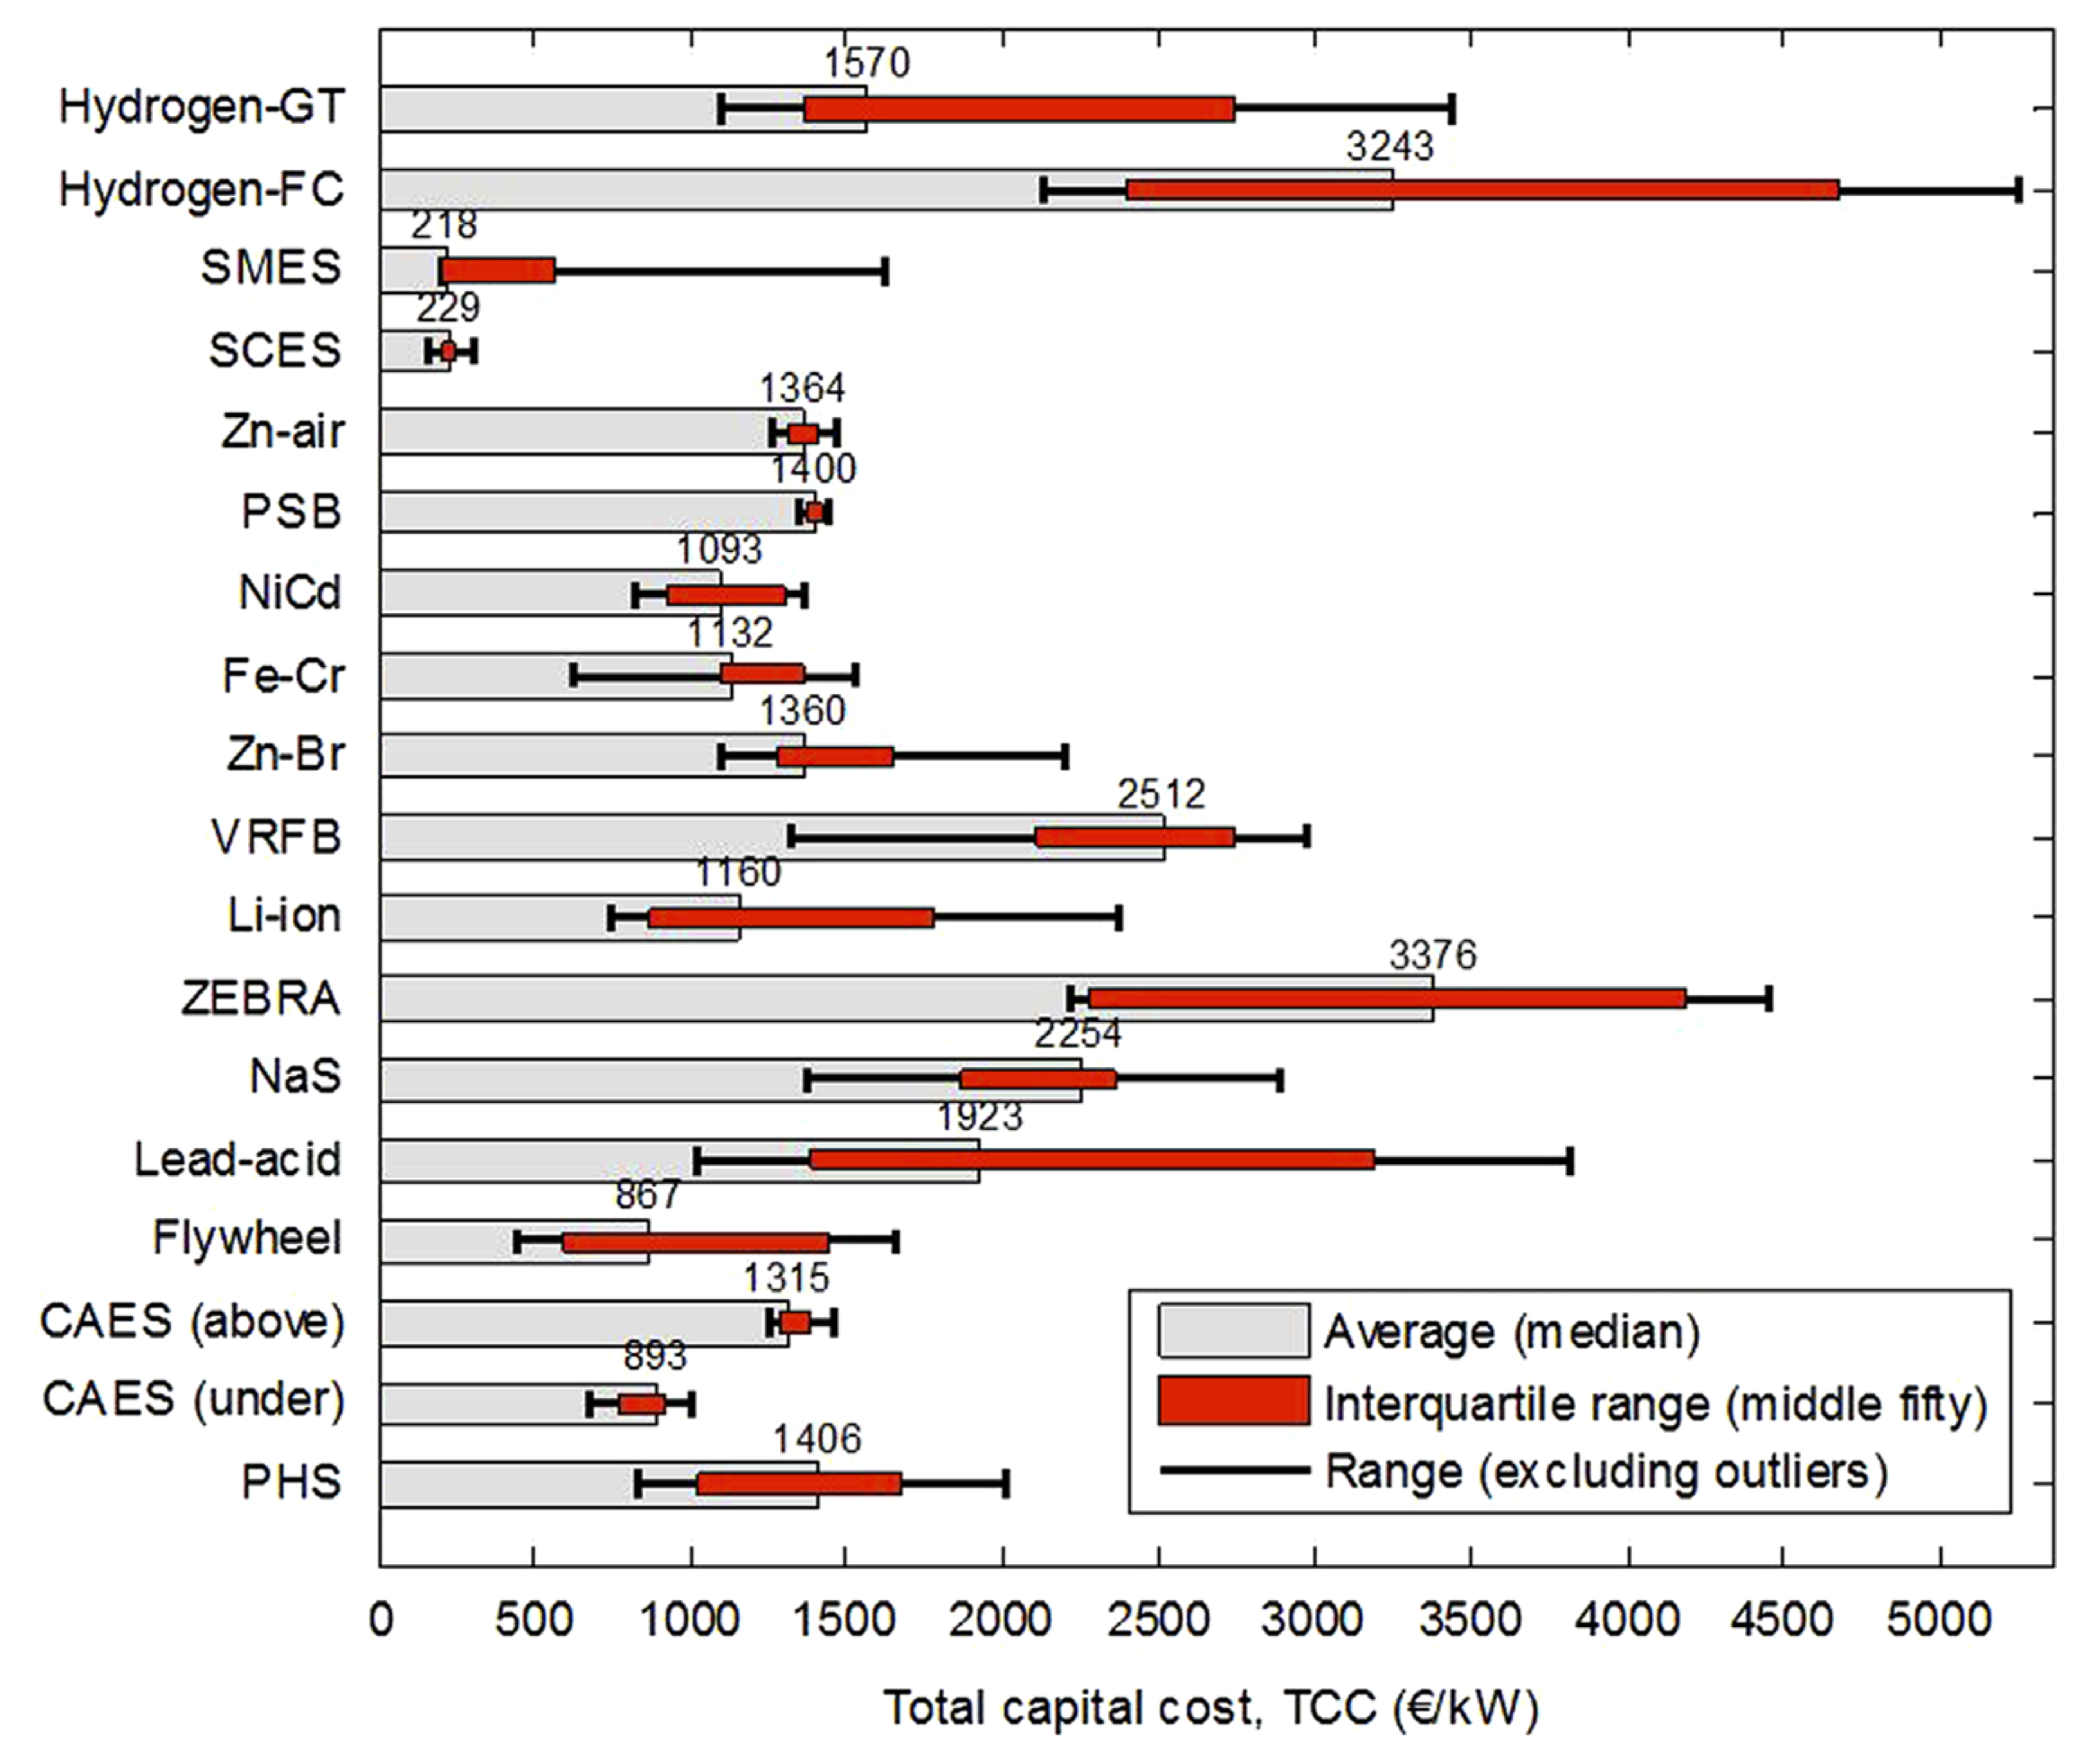
\includegraphics[width=0.65\linewidth]{FIG/TCC_EES}
\caption[Total capital cost in EUR of large-scale EES systems per unit of nominal power rating including costs of power electronics, storage part, fixed obtain and maintainence and maybe incidental replacement costs.]{Total capital cost in EUR of large-scale EES systems per unit of nominal power rating including costs of power electronics, storage part, fixed obtain and maintainence and maybe incidental replacement costs \cite{Zakeri2015}.}\label{TCC_EES}
\end{figure}
\pagebreak
\section{Impact of cost of capital on the levelised cost of solar power} \label{section WACC}
%Most low-carbon technologies in the power sector, specially solar and wind powered renewable, incur the main part of there cost up-front. They are costly to build but, thanks to cost free renewable source, comparative inexpensive to operate.
Low-carbon technologies in the electricity sector, especially solar and wind power, incur the biggest costs up-front. They are costly to build but, thanks to cost-free renewable source, comparatively inexpensive to operate.

%The weighted average cost of capital (WACC), which is a mix of the rate of return on capital and the interest rate for dept, at which the necessary capital and dept can be obtained is a crucial factor shaping the delivered cost of energy from solar technologies. The lower the WACC, the less expansive is energy from solar resources. In turn, factors that increase the WACC drive up the LCOE. In the case of an exemplary PV system, if the WACC exceeds \SI{9}{\percent}, finacing costs begin to dominate the LCOE of PV electricity (see Figure~\ref{WACC}). 

The \ac{WACC}, which is a combination of the rate of return on capital and the interest rate, is a crucial factor shaping the delivered cost of energy from solar technologies. The lower the \ac{WACC}, the less expensive energy from solar resources is. In turn, factors that increase the \ac{WACC} drive up the \ac{LCOE}. In the case of an example \ac{PV} system, if the \ac{WACC} exceeds \SI{9}{\percent}, financing costs begin to dominate the \ac{LCOE} of \ac{PV} electricity (Figure~\ref{WACC}).

\begin{figure}[htbp]  
\centering
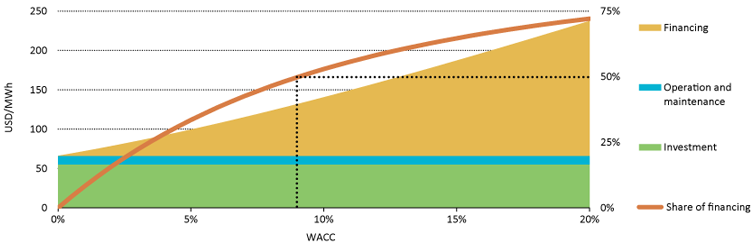
\includegraphics[width=1\linewidth]{FIG/WACC}
\caption[Impact of cost of capital on the levelised cost of an exemplary solar PV systems.]{Impact of cost of capital on the levelised cost of an exemplary solar PV systems \cite{IEA2015}.}\label{WACC}
\end{figure}
%Several factors influence the cost of financing. For technically mature technologies, the most relevant risk are those associated with the general investment climate in a market, the maturity of the local supply chain and the off-taker agreements. Depending on the policy, market and regulatory framework, investors may be exposed to substantial risk, which is bound to increase the WACC. \cite{IEA2014c} 

Several factors influence the cost of financing. For technically mature technologies, the most significant risks are those associated with the general investment climate in a market, the maturity of the local supply chain and the off-taker agreements. Depending on the policy, market and regulatory framework, investors may be exposed to substantial risk, which is bound to increase the \ac{WACC} \cite{IEA2014c}.

%The International Energy Agency calculates there LCOE for solar power applications (CSP and PV systems) with a WACC of \SI{8}{\percent} \cite{IEA2014c}. This also can be assumed for a EES application \cite{Zakeri2015}.

The \ac{IEA} calculates \ac{LCOE} for solar power applications (\ac{CSP} and \ac{PV} systems) with a \ac{WACC} of \SI{8}{\percent} \cite{IEA2014c}. This also can be assumed for a \ac{EES} application \cite{Zakeri2015}.

%As it was said, the WACC depends from the regional marked. For SA the WACC varied in 2013 from \SIrange{7.93}{8.89}{\percent} for onshore wind applications \cite{IEA2015}. For the subsequently simulation is a WACC of \SI{8}{\percent} for all solar power plants assumed.

The \ac{WACC} depends on the regional market. In South Africa, the \ac{WACC} varied in 2013 from \SI{7.93}{\percent} to \SI{8.89}{\percent} for onshore wind applications \cite{IEA2015}. For the simulation in this work, a \ac{WACC} of \SI{8}{\percent} for all solar power plants is assumed.

\section{General assumptions for a simulation-based comparison of large-scale solar power plants} \label{General assumptions}
To compare large-scale \ac{CSP} and \ac{PV} technologies, a simulated case study was performed on the basis of a \ac{CR} system, \ac{PTC} system and a \ac{PV} system with adapted \ac{EES}. Specific attention was given to maximizing daytime operation and meeting the prescribed demand curve as it was defined in Section~\ref{SystemloadinSA}. The \ac{PV} system was extended with battery storage. The storage capacity allocated for the simulation considerably exceeds the real capacity of electrical storage units currently available and is more than one-sixth the globally installed battery storage capacity of \SI{690}{GW} \cite{IEA2015}. Due to the scale and particularly with respect to the photovoltaic plant, the comparison is theoretical in nature.

With the aim of producing quantifiable and comparable results, the different solar supplied power plants were simulated using different input parameters. After that, selected comparable output parameters were analyzed, evaluated and rated.

The plant technologies selected for comparison are:
\begin{itemize}
\item \ac{CSP} molten salt central receiver with \acl{TES}
\item \ac{CSP} synthetic oil parabolic trough with \acl{TES}
\item \ac{PV} fixed elevated flat plate collectors with adapted \acl{EES}
\end{itemize}
The \ac{PV} plant has been extended with a \ac{li-ion} battery storage for the simulation, while the \ac{TES} of the \ac{CSP} plant uses molten salt technology. All plants were laid out for a maximum net power output of \SI{100}{\mega\wattel}. The plants are driven to match a prescribed load curve. In order to find an appropriate power plant design to match the load of the scenario, different layout parameters, using various storage and collecting field sizes, were tested. The location and related weather data for Upington was defined and described in Section~\ref{Solar radiation} for this simulation. The solar plants were implemented and simulated in \acp{NREL} \acf{SAM} version SAM 2015.6.30 r3 for OS X \cite{NREL2015}. \ac{SAM} is designed to simulate performance and financial models for different types of renewable energy. For this simulation, only the performance component was used. The financial analysis was done separately. 

The financial parameters and the resulting \ac{LCOE} are calculated separately for all power plants in Microsoft Excel 2011 (vers. 14.5.7) for Mac, using a simplified method using a lifetime of \SI{25}{years} for each plant (for details on the method, see Appendix~\ref{ChapterLCOE}, page \pageref{ChapterLCOE}).
%Nur noch zur Hilfe:
%\subsection{Parabolic-trough concentrating solar power} \label{subsection_PTC}
Parabolic trough power plants consist of many parabolic-trough-shaped concentrator that reflects direct solar radiation onto a receiver or absorber tube (also called receiver tube) located in the focal line of the parabola. The heated fluid is used in a steam generation system, to drive a steam turbine/generator cycle. Optional thermal storage and/or fossil-fired backup systems are possible. A schematic concept of a parabolic trough power plant is shown in Figure \ref{parabolic_troughs}. The collector field is made up of a large number of single-axis-tracking parabolic trough solar collectors and receivers. The solar field is modular in nature and comprises many parallel rows of solar collectors, normally aligned on a north-south horizontal axis. The collectors track the sun from east to west during the day to ensure that the sun is continuously focused on the linear absorber tube.
\begin{figure}[!h] 
\centering
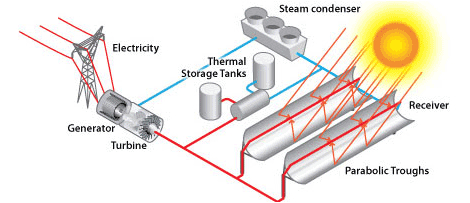
\includegraphics[width=0.7\linewidth]{FIG/parabolic_troughs}
\caption[Schematic parabolic trough power plant concept.]{Schematic parabolic trough power plant concept \cite{U.S.DOE2013}.}\label{parabolic_troughs}
\end{figure}


The first graphically documented parabolic-trough solar collector was designed and built in 1870 by Swedish engineer John Ericsson. This collector produced 373~W by a steam engine had and had a solar radiation collecting surface of 3.25~m$^2$. \cite{Fernandez-Garcia2010}

Current PTC are based on developments in the united states which began after the first oil crisis. In the 1980s the first commercial used PTC plants was build. Most outstanding the implementation of the nine SEGS (Solar Electricity Generating System) plants. Build from 1984 (SEGS-I) to 1990 (SEGS-IX) in the Mohave Desert (California, USA) by LUZ International Limited and still operating. In total they have an electrical output of 354 MW and more than two million square meters of parabolic-trough collectors. They using oil to produce steam in heat exchangers before being circulated back to the solar field. Like in a electricity generating plant the steam is used in a conventional steam turbine. After the cutting down of government incentives for renewable systems and the oil price fell again in the 1980s the installation of more SEGS plants went unfeasible. \cite{Kalogirou2014a}

But the technology is still applied in most of the present build commercial parabolic trough power plants. Today they are using as HTF synthetic oil, typically out of biphenyl/diphenyl oxide fluid. The maximum cycle temperature is limited to values below 400$\,^{\circ}\mathrm{C}$ in order to avoid decomposition of the HTF. The thermal energy from the solar field is transported by the HTF to the heat-exchanger steam generator systems providing the superheated steam for the turbine of typically 370-380$\,^{\circ}\mathrm{C}$. The limitation of the upper process temperature to about 400$\,^{\circ}\mathrm{C}$ can be overcome by changing the HTF. A higher process temperature leads to a significant increase in the thermodynamic conversion cycle efficiency. A summary of current applied HTFs can be found in Chapter~\ref{subsection_HTF}.

An alternative HTF is water/steam, which is used in the steam cycle any way. The direct steam generation (DSG) in parabolic trough collectors demonstration loops steam reaches temperature of 550$\,^{\circ}\mathrm{C}$. Aside from the process temperature, the benefits of DSG compared with oil are based on savings in the heat exchanger, in reduced pumping effort, and the uncritical handing of the medium. But there are still barriers for commercial scale application. Some of the most important technological challenges of the DSG parabolic trough plant are the control stability, receiver tube viability, and collector interconnection feasibility.  \cite{Alguacil2014}

Another alternative HTF for PTC is molten salt. Salts already proved there competence in solar tower power plants and also application of liquid salts in parabolic trough systems have been investigated. Salts has suitable thermophysical properties, namely high boiling and decomposition point, low vapor pressure, high specific heat capacity, high thermal conductivity, and high density at low pressures \cite{Cordaro2011}. Molten salt has also the advantage to be the art of science in thermal storage for large- scale CSP plants (see Chapter \ref{Subsection_storage_system}).  Furthermore, typical salt mixtures are significantly cheaper than synthetic oils \cite{Gil2010}. The 5~MW Archimede commercial PTC plant is using a mixture of sodium nitrate (60\%) and potassium (40\%) nitrate since 2010 \cite{NREL2012}. The upper solar-field outlet temperature is 550$\,^{\circ}\mathrm{C}$ but starts crystallization of the non-eutectic melt occurs at 238$\,^{\circ}\mathrm{C}$ \cite{Cordaro2011}. That is one concerns with molten salt-based parabolic trough plants. The solar plant needs to be fully equipped with impedance and trace heating systems in order to ensure non-freezing of the salt. Therefore also the the process setup needs to be modified. But according to the researcher of the "Archimede Solar Energy molten salt parabolic trough demo plant" the molten salt parabolic trough (MSPT) technology is mature for large scale commercial applications without any critical points to be addressed \cite{Maccari2015}. Also the higher investment costs in solar field and piping, as well as maintenance and operation cost seams to be manageable and will be overcome to the increase in total plant efficiency and lower storage and HTF costs. Therefore the expected levelized cost of electricity (LCoE) of PTC power plants will decrease around 20\% \cite{Richert2015}. Component manufacturers are starting to introduce products specifically aimed at this technology. Upcoming projects needs to validate this expected decrease of LCoE in commercial scale and represent their profitability. \\ 


As mentioned above a PTC power plant consists out of the components collector and receiver, which held together by support structure. This components are connected in loops, which building the solar field.
\subsubsection{Parabolic Trough Collectors}
The task of PTC module is to reflect the radiation of the sun accurately to the receiver tube. So the main components of a PTC module are actually the curved mirror and the absorber tube. But usually the PTC means the reflector and its support structure. The absorber tubes are separately regarded. The structure holds the components in place and connects the reflector modules between each other. To concentrate the radiation to the absorber tube the shape of the reflective surface is in parabolic form like in Figure \ref{PTC_section}. There shown is a section of a PTC with the dimensions of the commercial used LS-3, EuroTrough and Senertrough-1 and their focus point. This focus point is only at this position when the z-axis is in the direction of the Sun. Therefor the PTC is controlled by means of astronomical calculations, often supplemented by a Sun position sensor. The absorber tubes mounted in the focal line move with the collector and are connected to the stationary field piping via flexible hoses or rotating joint arrangements.
\begin{figure}[!h] 
\centering
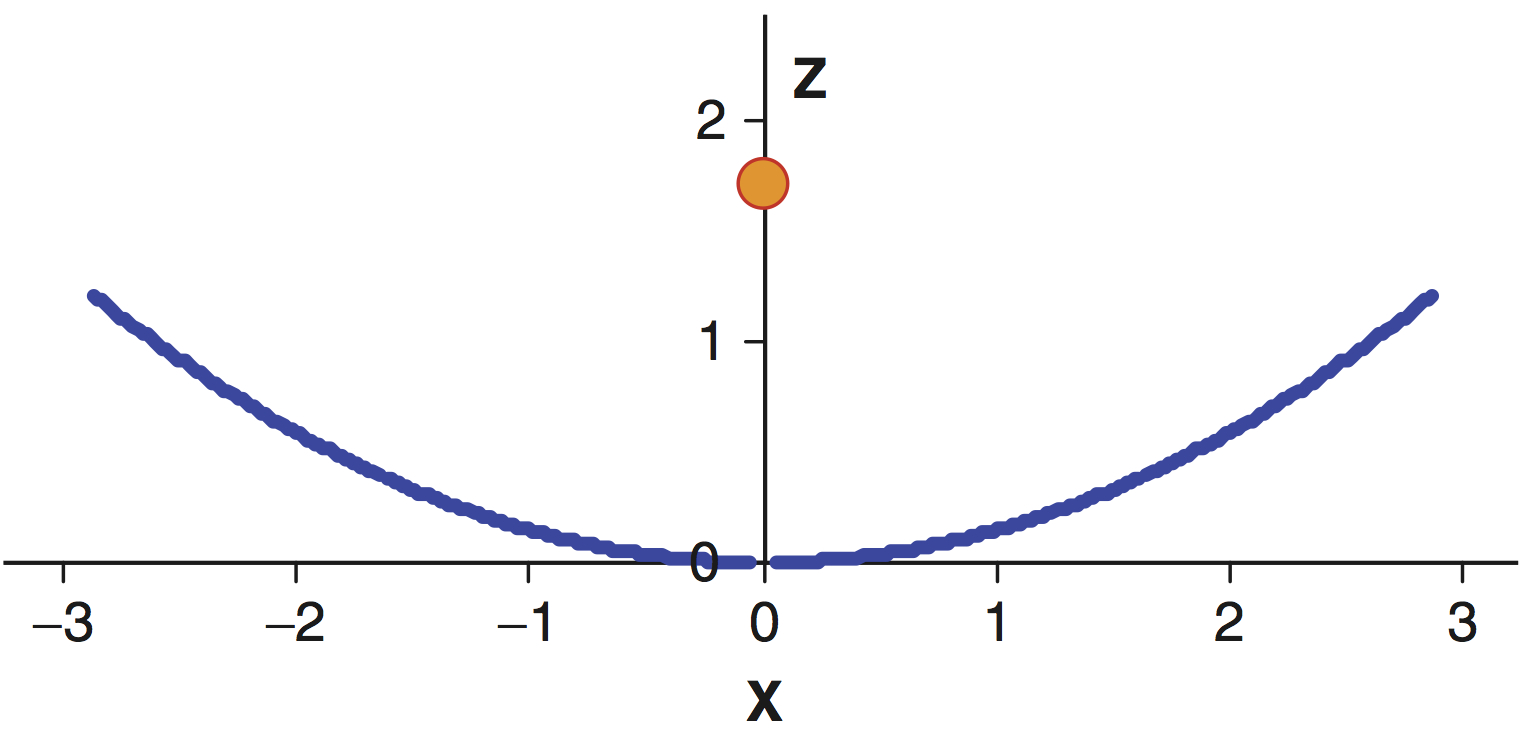
\includegraphics[width=0.6\linewidth]{FIG/PTC_section}
\caption[PTC section – dimensions of EuroTrough, LS-3, and other designs, in meters.]{PTC section – dimensions of EuroTrough, LS-3, and other designs, in meters \cite{Lupfert2013}.}\label{PTC_section}
\end{figure}


The history of PTC goes far back to 1870, where they already used small engines with solar power \cite{Fernandez-Garcia2010}. With the time of the first oil crisis in the 1980s also new PTC were developed. In this decade also the collector family LS-1, LS-2 and LS-3 was developed by LUZ. These PCT  were implement in the first large-scale solar thermal power plants SEGS 1 (1984) to SEGS 9 (1990) in California. The used PTC features a modular design based on steel structures with parabolic preshaped, silvered glass mirrors and improved efficiency by implementation of evacuated tube receivers. A European consortium designed in the late 1990s the EuroTrough. Which was based on the LS-3 concentrator geometry with a focal length (the shortest distance from the mirror to the focal line) of 1.71~m and an aperture (the projection of the concentrator area in the direction of the optical axis) width of 5.77~m, but offered advantages in stiffness and costs \cite{Osuna2001}. Some years later, SENER developed a different structural approach, but still maintained the basics of LS-3 concentrator geometry \cite{Fernandez-Garcia2010}.
\begin{figure}[!h] 
\centering
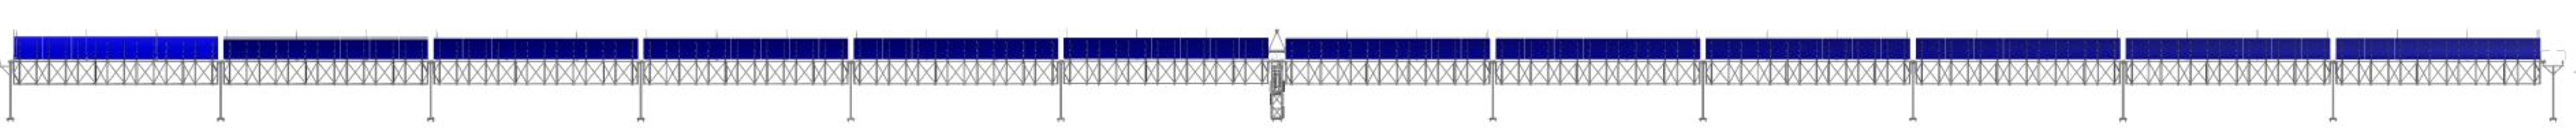
\includegraphics[width=1\linewidth]{FIG/SCA_EuroTrough}
\caption[Solar Collector Assembly (SCA) composed of 12 EuroTrough collector elements (SCE).]{Solar Collector Assembly (SCA) composed of 12 EuroTrough collector elements (SCE) \cite{VonReeken2014}.}\label{SCA_EuroTrough}
\end{figure}


PTC are typically assembled from solar collector element (SCE), mounted on a series of aligned pylons. The center pylon is equipped with a hydraulic drive system to allow tracking of the total solar collector assembly (SCA). Figure~\ref{SCA_EuroTrough} shows the SCA of the EuroTrough. From 12 SCE of the SCA results a total length of approximately 150~m and 816~m$^2$ \cite{VonReeken2014}. 

Table \ref{tbl: TroughCharacteristics} illustrates that recent developments show a continuing trend towards larger aperture sizes such as for the Heliotrough, Senertrough-2 and Ultimate Trough. The development steps of the aperture size are exemplary shown in Figure \ref{Kollektoren} for EuroTrough, Heliotrough and Ultimate-Trough. 

\begin{table}[h!]  
  \centering
	\begin{tabular}{  p{3.3cm}  C{1.0cm}  C{1.0cm}  C{1.5cm}  C{1.0cm}  C{1.0cm}  C{1.0cm}  C{1.0cm}  C{1.5cm}} 
\hline
\textbf{Property} & \textbf{LS-1} & \textbf{LS-2} & \textbf{LS-3} & \textbf{Euro-Trough} & \textbf{Helio-trough} & \textbf{Sener-trough-1} & \textbf{Sener-trough-2} & \textbf{Ultimate-Trough} \\ \hline \hline
Start of development & 1984 & 1985 & 1989 & 1998 & 2005 & 2005 & 2006 & 2009 \\ \hline
Aperture width [m] & 2.55 & 5.00 & 5.77 & 5.77 & 6.78 & 5.77 & 6.87 & 7.51 \\ \hline
Length per module/SCE [m] & 6.3 & 8 & 12 & 12 & 19 & 12.27 & 13.23 & 24 \\ \hline
SCA length [m] & 50.2 & 47.1 & 99 & 147.8 & 191 & n.a. & 158.8 & 242.2 \\ \hline
Focal length [m] & 0.68 & 1.40 & 1.71 & 1.71 & 1.71 & 1.71 & 2 & n.a. \\ \hline
\end{tabular}
\caption[Characteristics of different parabolic trough collectors.]{Characteristics of different parabolic trough collectors \cite{Pitz-Paal.2013}.}\label{tbl: TroughCharacteristics}
\end{table}


The use of lager collector units with more aperture area brings some advantages. The Ultimate Trough shows a cost reduction of about 20 to 25\% compared to the EuroTrough. Coming from lower specific costs and increased of optical performance. Also the amount of heat transfer fluid can be reduced by 25\%. This promise an decreased LCoE by about 11\% compared to EuroTrough. \cite{VonReeken2014}
\begin{figure}[!h] 
\centering
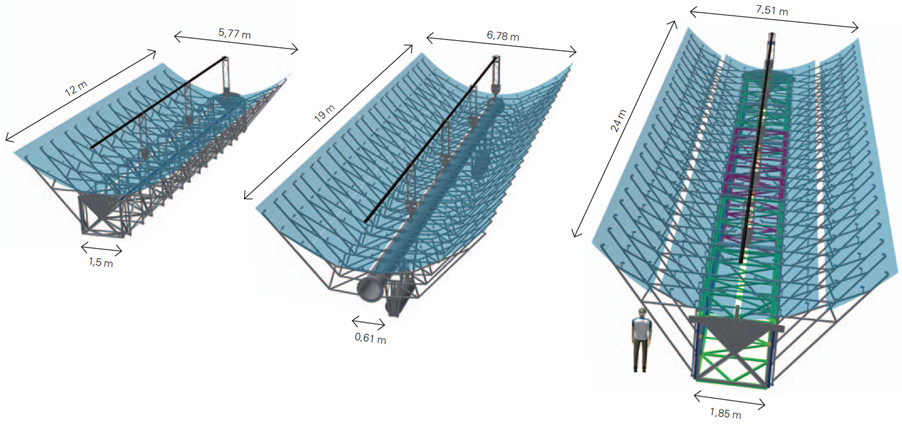
\includegraphics[width=1\linewidth]{FIG/Kollektoren}
\caption[Evolution of parabolic trough collector sizes over 3 development cycles (Eurotrough, HelioTrough, Ultimate Trough).]{Evolution of parabolic trough collector sizes over 3 development cycles (Eurotrough, HelioTrough, Ultimate Trough)\cite{Schlaichbergermannundpartner}.}\label{Kollektoren}
\end{figure}


Another approach to reduce costs is the utilization of other reflector materials. The Skytrough uses reflectors made from silvered polymer film laminated to aluminum sheets mounted on a space frame. Compared the to the costs of components of the EuroTrough, the Skytrough contribute an additional 34\% cost savings in combination with a aperture width of 6.0~m \cite{Mason2014}. Thin glass on a glass-fiber/foam sandwich was used for the SL4600 construction \cite{SolarliteCSPTechnologyGmbH2014}. Both approaches take advantage of the mechanical strength of the mirrors to reduce the amount of additional steel structure required.

Abengoa Solar is developing currently the "SpaceTube" concept, using 8~m aperture width and will use 80~mm diameter absorber tubes. \cite{Olar2013}
\pagebreak
\subsubsection{Absorber tube (Receiver)}
The absorber tube or also called receiver is the component where solar energy is converted to thermal energy in the form of sensible or latent heat of the fluid that circulates through it. This component produces the predominant share of thermal losses in an parabolic trough power plant, for that reason it is also one of the most critical and important performance components \cite{Lupfert2013}. Currently, there are just two types of receiver for parabolic trough power plants, classified as either evacuated or non-evacuated. Evacuated receivers are commonly used for temperatures above 300$\,^{\circ}\mathrm{C}$ and its consist of three main parts. The metal absorber tube, an protection glass tube and the connection unit with expansion bellows. In order to reduce thermal losses and increasing the overall efficiency of the PTC the receiver unit uses a high vacuum (i.e.,~10-5~mbar) between the metal absorber tube and the protection glass. Figure shows \ref{absorber_tube} the structure of an typical vacuum tube receiver. 
\begin{figure}[!h] 
\centering
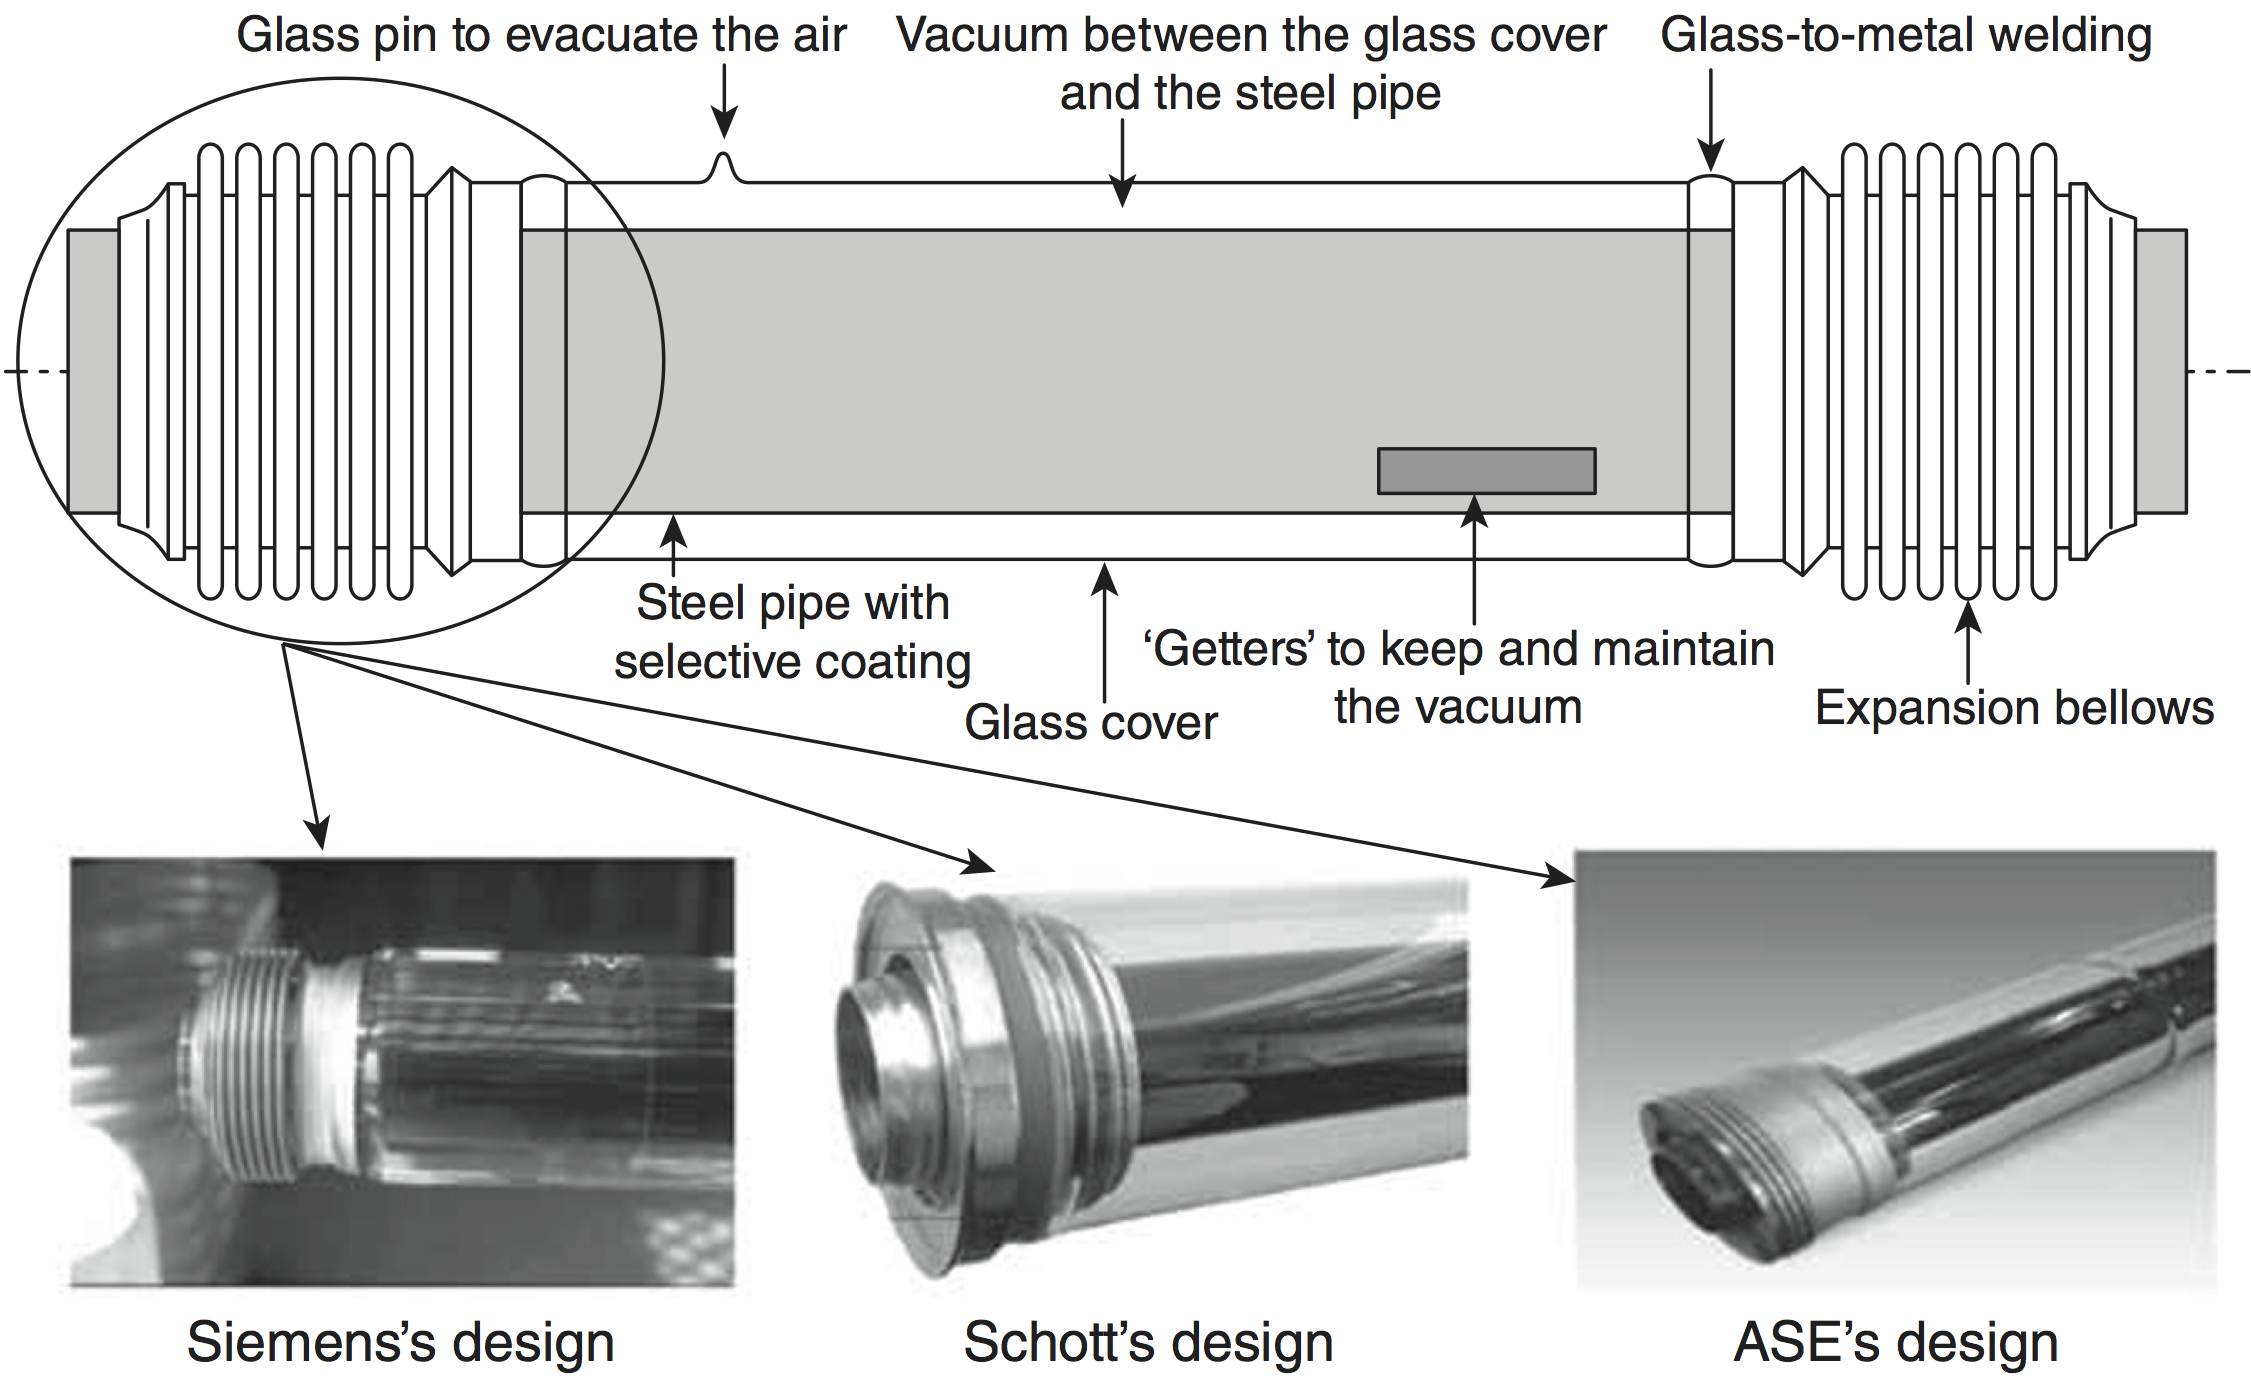
\includegraphics[width=0.9\linewidth]{FIG/absorber_tube}
\caption[A typical evacuated receiver for parabolic-trough collectors.]{A typical evacuated receiver for parabolic-trough collectors \cite{Moya2012}.}\label{absorber_tube}
\end{figure}
\\

The metal absorber tube is a dark-coated to absorb the incoming solar radiation. It absorbs the concentrated radiation reflected from the mirror, and also the global radiation hitting from top. The outer surface of the metal absorber tube has an optically selective surface with a high solar absorptance and low emittance for thermally generated infrared radiation. This is achieved with sputtered Cermet coatings consisting of several layers of metallic and ceramic coatings. Also, galvanic black-nickel and black-chrome coatings are applied but have less temperature resistance and higher emissivity. \cite{Platzer2012}



The protection glass is connected to the metal absorber tube by means of stainless steel expansion bellows. These bellows compensate the thermal expansion of glass and steel which results at nominal working temperature. Therefore one end of these expansion bellows is directly welded to the outer surface of the metal absorber tube, while the other end is connected to the end of the protection glass by means of a glass-to-metal welding. The glass-to-metal welding is a weak point in the absorber system and has to be avoid by high thermal and mechanical stress that could cause the welding to crack. The receiver provider has various solution for the expansions bellows. Figure \ref{absorber_tube} shows also the solutions of three manufacturers (Schott, Siemens and ASE) joining the protection glass and the inner metal absorber tube. The expansion bellows also provide a tight annular gap between both tubes to make the vacuum. To support the shelf life of the vacum chemical ‘getters’ can be placed in the gap between the metal absorber tube and the protection glass to absorb gas molecules.
\begin{table}[!h]  
  \centering
	\begin{tabular}{  p{3.5cm}  C{3.5cm}  C{3.5cm}  C{3.5cm} } 
	
	\hline	
 & \textbf{Schott PTR-70} & \textbf{Siemens UVAC-2010} & \textbf{ASE HEMS08}\\ \hline \hline

Solar absorptance & $\ge$~0.95 & $\ge$~0.96 & $\ge$~0.95 \\ \hline
Solar transmittance & $\ge$~0.96 & $\ge$~0.96 & n.a. \\ \hline
Thermal emittance & $\le$~0.1 at 400$\,^{\circ}\mathrm{C}$  & $\le$~0.9 at 400$\,^{\circ}\mathrm{C}$& $\le$~0.1 at 400$\,^{\circ}\mathrm{C}$  $\le$~0.14 at 580$\,^{\circ}\mathrm{C}$\\ 
Steel pipe inner/ outer diameters & 70/65~mm stainless steel & 70/65~mm stainless steel & 70/65~mm stainless steel \\ \hline
Thermal losses & 250 W/m at 400$\,^{\circ}\mathrm{C}$ & n.a. & 230 W/m at 400$\,^{\circ}\mathrm{C}$ \\ \hline
Glass cover & Borosilicate & Borosilicate & Borosilicate\\ \hline
Active length ratio at 350$\,^{\circ}\mathrm{C}$ & >96\% & 96.4\% & n.a.\\ \hline
Maximum fluid temperature & 400$\,^{\circ}\mathrm{C}$ & 400$\,^{\circ}\mathrm{C}$ & 550$\,^{\circ}\mathrm{C}$\\ \hline
\end{tabular}
\caption[Technical parameters of the receivers commercialized by Schott, Siemens and ASE.]{Technical parameters of the receivers commercialized by Schott, Siemens and ASE \cite{Moya2012}.}\label{tbl: receiver_details}
\end{table}
\\

Most of the parabolic-trough solar thermal power plants implemented around the world until 2009 had receivers manufactured by either the Israeli company, Solel (purchased in 2009 by Siemens and 2013 from Abengoa \cite{Alcauza2013}), or the German company, Schott. In 2009, the Italian company, Archimede Solar Energy (ASE), announced that they were launching a new receiver tube called HEMS08, suitable for fluids up to 550$\,^{\circ}\mathrm{C}$. The first plant using HEMS08 receivers was the Archimede Plant, located in Syracuse (Italy) and ready to operate in 2010 using molten salt as HTF. Most widespread geometry is the receiver, with 70~mm absorber tube diameter, but due to larger aperature width of the trough reflectors, also the absorber tube diameter is raising. The technical details of the receivers manufactured 2012 by Schott, Siemens and ASE are shown in Table \ref{tbl: receiver_details}. Schott's PTR-70 is now in the 4. generation, the actual UVAC 70-7G is now in production by Rioglass a subsidiary from Abengoa Solar and ASE's present molten salt receiver tube is the HCEMS-11, but in generally the technical parameters are still up-to-date \cite{Schott2015,ArchimedeSolarEnergy2015,RioglassSolarInternational2014}.
\\

Most widespread geometry is the receiver, with 70~mm absorber tube diameter, but due to larger aperature width of the trough reflectors, also the absorber tube diameter is raising. This is a further contribution to using molten salt as future HTF in large-scale PTC power plants. 
\pagebreak
\subsubsection{Field}
The heat-collecting portion of the PTC power plant is the solar field. It consists of one or more parallel loops of SCAs. A common header pipe provides each loop with an equal flow rate of HTF. A second header collects the hot HTF to return it either directly to the power cycle for power generation or to the thermal energy storage system for use at a later time. To minimize pumping pressure losses, the field is typically divided into multiple sections, each section with its own header set, and the power cycle is situated near the middle of the field. The size of the field depends on required thermal power for the power block and the storage system. The orientation of the field depends obviously on the orientation of the parabolic collectors, which are installed with their north-south oriented rotation axis.
\begin{figure}[!h] 
\centering
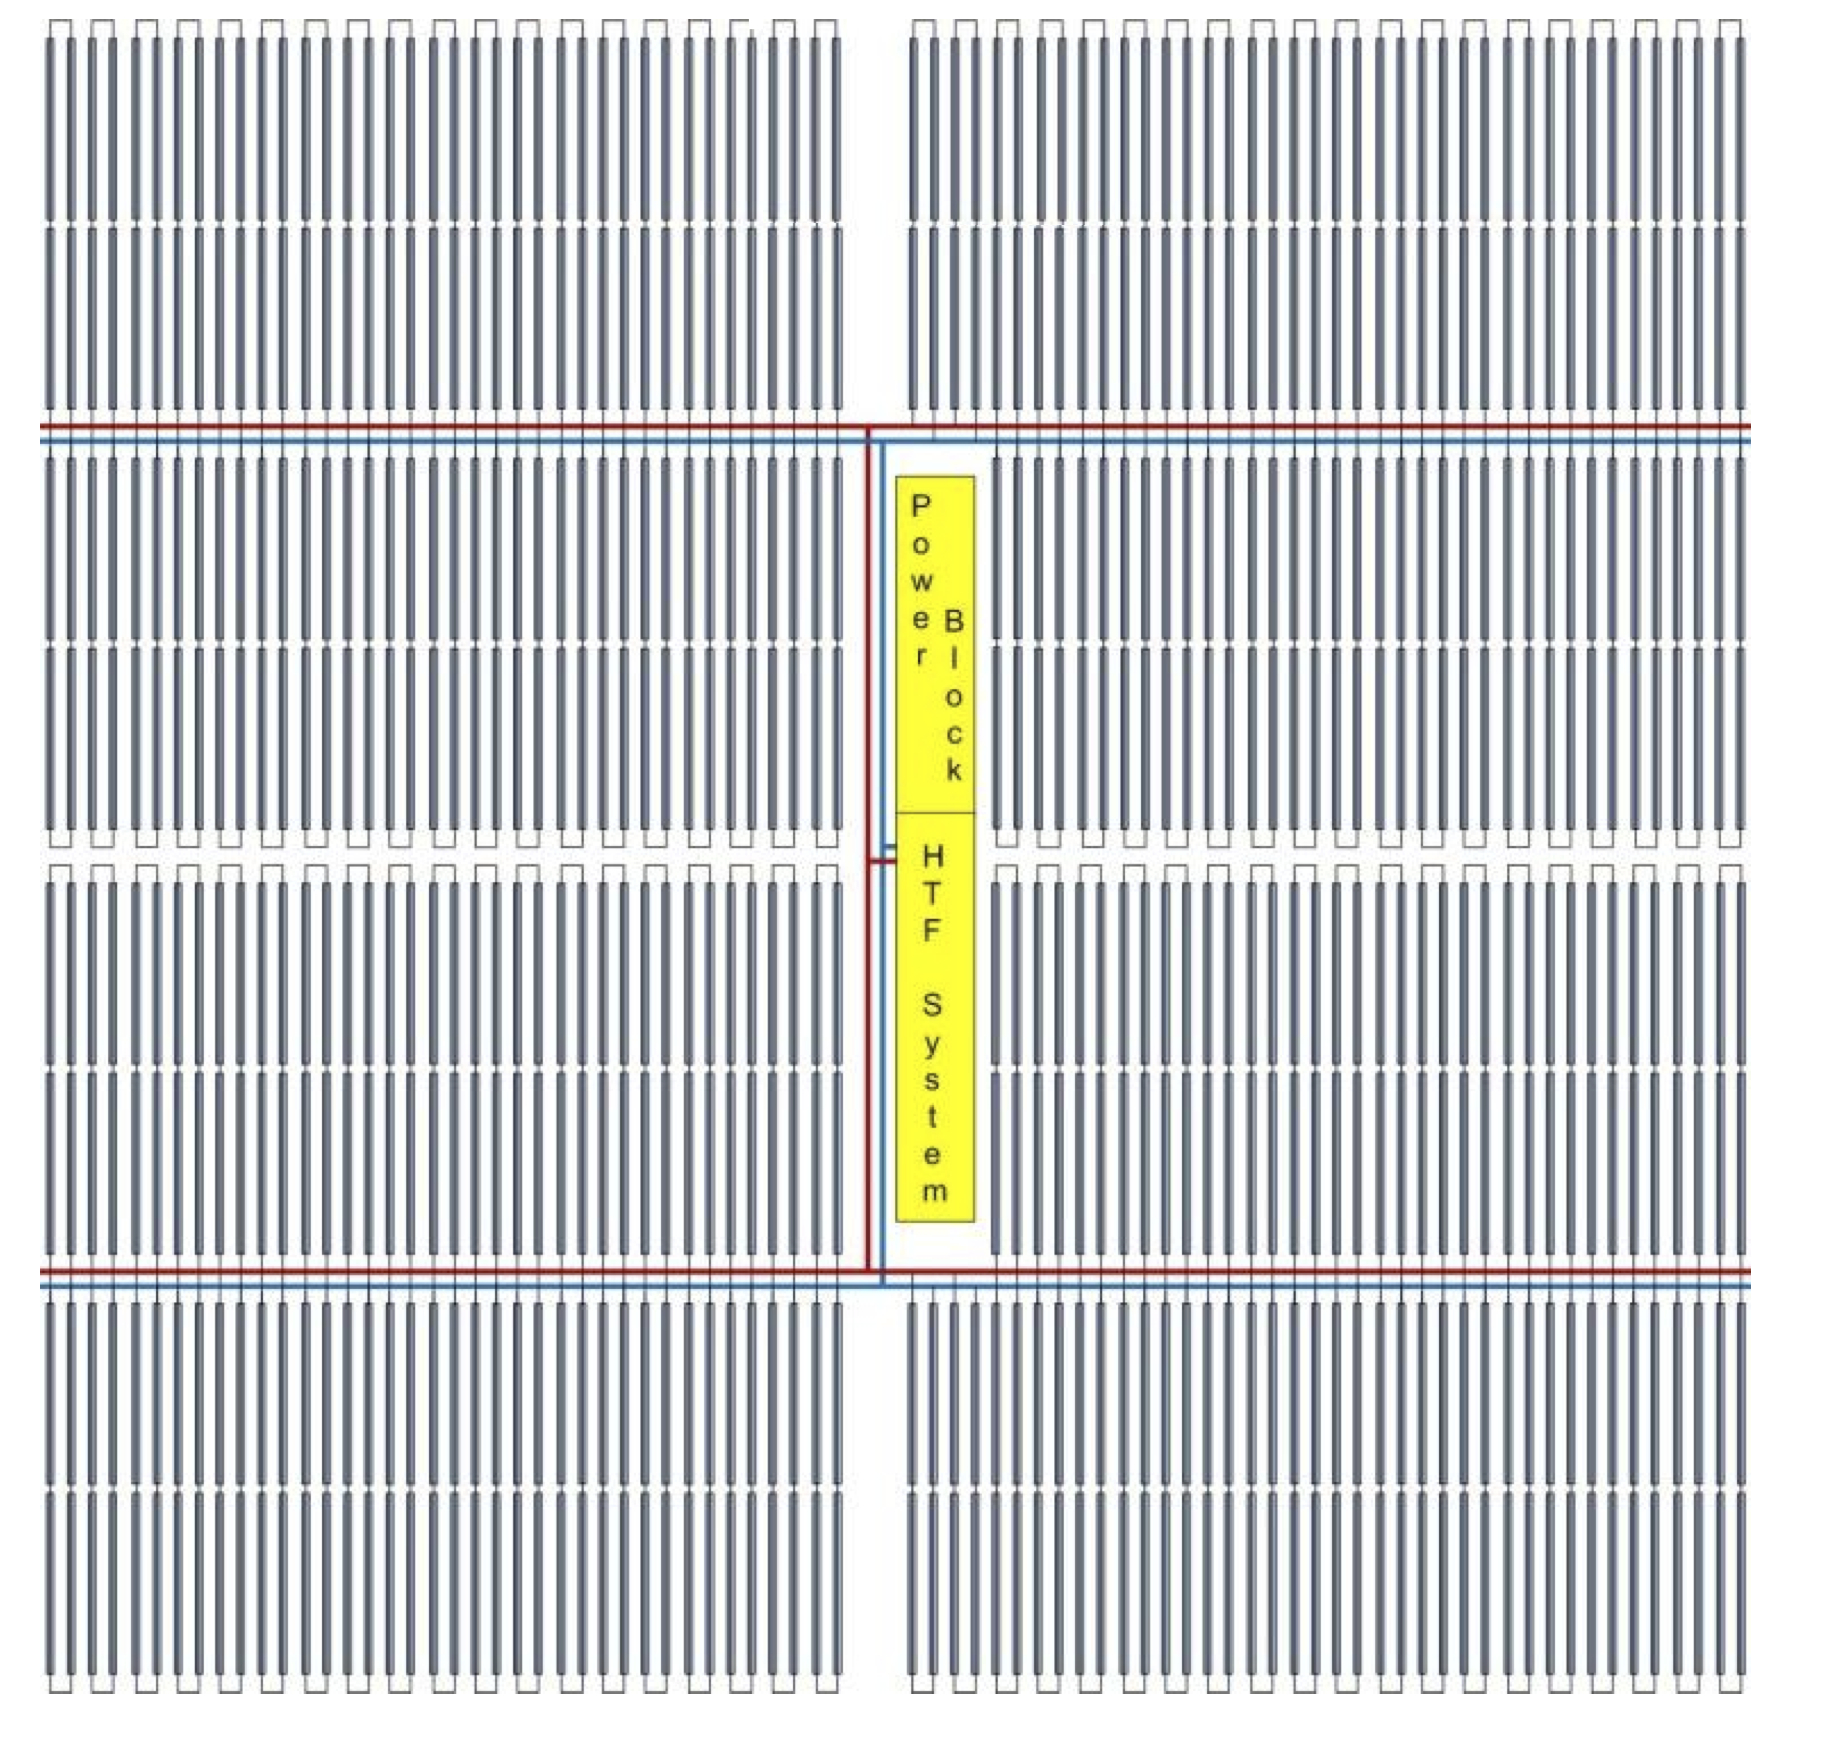
\includegraphics[width=0.7\linewidth]{FIG/PTC_field_EuroTrough}
\caption[Example of a EuroTrough collector field layout with 152 loops.]{Example of EuroTrough collector field layout with 152 loops \cite{VonReeken2014}.}\label{PTC_field_EuroTrough}
\end{figure}
Figure \ref{PTC_field_EuroTrough} shows one example plant layout for where  152 total loops are used, each loop with four SCA. The loop length depends on heat transfer fluid properties and rise in temperatures between inlet and outlet temperature ($\Delta T$). The flow rates through the receivers must be high enough to ensure appropriate heat removal from the absorber walls and low enough to keep pumping power for the fluid reasonably low.
\pagebreak
\subsubsection{Current stage of commercial scale PTC power plants}
On the commercial  scale the "Solana Generating Station" is currently one of the world largest PTC power plants. It was built from December 2010 to October 2013 southwest of Phoenix, Arizona. The solar-field aperture area of 2~200~000~m$^2$ concentrates in 808 loops with 4 SCA per loop drives two 140~MW$_{el}$ turbines. This plant uses synthetic oil as HTF and has a storage capacity of 6~h in molten salt (described in Chapter \ref{Subsection_storage_system}). The fed-in tariff of approx. 944~GWh/a is fixed for 30 years. The costs of the plant were approx. 2 USD billion. This power plant constitutes the current state of art in commercial scale PTC systems. \cite{NREL2015d}
\begin{figure}[!h] 
\centering
\includegraphics[width=1\linewidth]{FIG/PTC_Solana}
\caption[280-MW Solana PTC power plant near Phoenix, Arizona.]{280-MW Solana PTC power plant near Phoenix, Arizona \cite{AbengoaSolar2013a}.}\label{PTC_Solana}
\end{figure}
\pagebreak
\subsection{Central tower concentrating solar power} \label{subsection_CRS}
Central receiver systems (CRS) use a large number of reflectors (heliostats) to concentrate direct solar radiation to a focal point, in most cases on top of a tower. In order to reflect the incident sunlight to the focal point, the heliostats are tracked in two dimensions. The receiver is located at the focal point. The receiver absorbs the concentrated solar radiation and heats a HTF, such as a liquid or a gas. The generated heat drives a turbine to produce electricity by a generator. The basic principle of a solar CR power plant is shown schematically in Figure~\ref{power_tower}. Average concentration levels on the receiver are typically in the range 500-1~000 kW/m$^2$ \cite{Pitz-Paal.2013}. This concentration level is significantly higher than those achievable in linear focus systems such as PTC systems. The higher concentration level enables higher operational temperatures in the receiver, while maintaining good thermal efficiencies.
\begin{figure}[!h] 
\centering
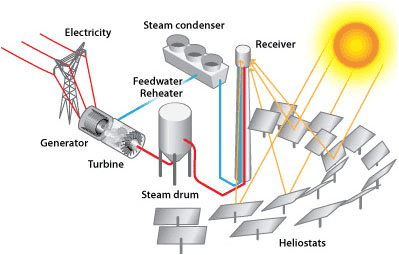
\includegraphics[width=0.6\linewidth]{FIG/power_tower}
\caption[Schematic CR power plant concept.]{Schematic CR power plant concept \cite{U.S.DOE2013}.}\label{power_tower}
\end{figure}


A variety of solar tower concepts exist or are under development. These concepts differ mainly in the type of heat transfer medium, which dominates the layout and selection of all other components except for the heliostat field. Liquid or gaseous HTFs are state-of-the-art in solar tower technology. Water/steam, molten salt, and air are typical fluids \cite{Pitz-Paal.2013}. A HTF in a central receiver absorbs the highly concentrated radiation reflected by the heliostats and converts it into thermal energy to be used for the subsequent generation of superheated steam for turbine operation. The different HTF mediums are described in  chapter \ref{subsection_HTF}. Not like the more or less uniform design of PTC systems is the optical design and optimization of CRS more complicated. A multitude of variables one must be consider such as the continuous variation in configuration and performance of each of the heliostats as they track the sun and interact with one another. 

The first documented concept of using ground-based segments (heliostats) to reflect direct-beam sunlight on a receiver comes from the Russian Victor Baum \cite{Baum1957}. But at this point no experimental device was built.

After several central receiver concepts and first 'commercial' used heliostats \cite{Trombe1957}, Alvin Hildebrandt published in 1972 the basic concept of nowadays CR systems as a hemispherical or cylindrical receiver atop a tall tower surrounded by a field of carefully positioned heliostats. The described power plant should have a tower height of 450~m with an heliostat field of 1.8~km diameter and produce 565~MW$_{th}$. There were no technical impediments expected with the tower or heliostat field. \cite{Hildebrandt1972}

Outgoing from more basic concepts and further research the Solar One, a 10~MW$_{el}$ CR ‘pilot plant’ was operated successfully from 1982 to 1988, in the desert near Barstow, California. This facility used a cylindrical receiver with water-steam as HTF at the focal point in 76~m height. The tower was surrounded by 1~818 heliostats, each with almost 40~m$^2$ area. After several problems in terms of storage and continuous turbine operation, the Solar One was upgraded to the Solar Two using molten salt as HTF and as direct storage concept. The Solar Two operated from 1996 to 1999 pumping molten nitrate salt at 290$\,^{\circ}\mathrm{C}$ from a cold storage tank through the receiver, where it was heated up to approximately 565$\,^{\circ}\mathrm{C}$ and afterwards to a storage tank, which had a storage capacity of 3~h. A simplified scheme of the Solar Two system is shown in Figure~\ref{towerdirecttwotank} on Page~\pageref{towerdirecttwotank}. \cite{Reilly2001}

The Planta Solar 10 (PS10) is the first solar central-receiver system producing grid-connected electricity under a purely commercial approach and started generating 11~MW$_{el}$ in 2007 near Seville, Spain. 624 heliostats with surface area of 120~m$^2$ each, concentrates direct irradiance to a cavity receiver using saturated steam as HTF on top of a 115~m high tower. The function of the PS10 is schematically shown in Figure~\ref{directsteamgeneration}.
\begin{figure}[!h] 
\centering
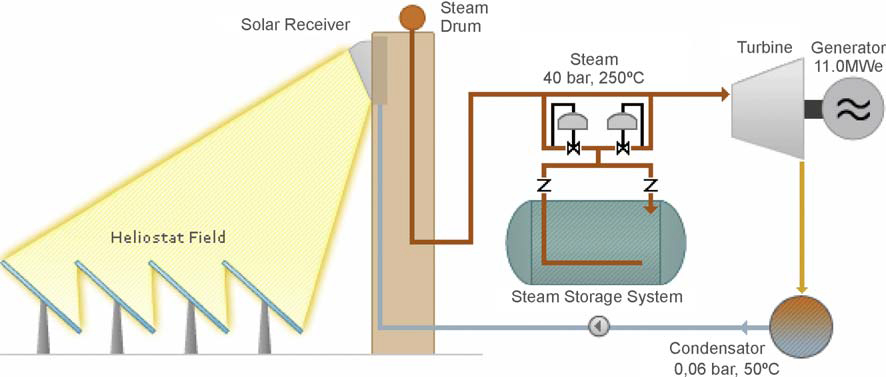
\includegraphics[width=0.7\linewidth]{FIG/directsteamgeneration}
\caption[Schematic diagram of the PS10 solar tower using water/steam as HTF.]{Schematic diagram of the PS10 solar tower using water/steam as HTF \cite{Medrano2010}.}\label{directsteamgeneration}
\end{figure}


The first commercial solar thermal power plant to supply uninterrupted power for a full 24~h is the 19.9~MW$_{el}$ Gemasolar power plant, which started operation also near Seville in 2011. 2~650 heliostats focusing on the tube receiver on top of a 140~m height tower. The molten salt, which is used as HTF and for storage, reaching temperatures of 565$\,^{\circ}\mathrm{C}$.

Current commercial planned large-scale CR power plants are based on the PS10 and the Gemasolar power plant. Their main components are the heliostats and their field design, the receiver, and the tower itself. These are described bellow. Chapter \ref{Subsection_storage_system} examined the storage possibilities.  \pagebreak
\subsubsection{Heliostats}
Current heliostat technology differs mainly in the area of the reflecting surface. Studies of the heliostats area reaches from 1.1~m$^2$ up to 320~m$^2$ \cite{Tyner2014,Blackmon2012}. One of the largest heliostats in commercial application will have a total area of 140 m$^2$ \cite{Abengoa2014} and are built of several smaller facets, mounted on a back structure. Classical heliostat design is dominated by mirrors brought into position by steel structures and drives that guarantee high accuracies under wind loads and thermal stress situations. To the structures that hold the mirrors include struts, beams, the pylon, and the foundation. The linear actuators enable moving of the heliostat in two dimensions. There exists a zenith and an azimuth actuator together with their step motors. The orientation of the rotation axes may also differ between heliostat types. Several different types of heliostat mirrors exist. They can be differentiated according to size, shape, basic design concept, or even according to there tracking system. Each heliostat type has its own characteristics in terms of wind-performance and tracking during windy conditions, costs, and complexity of control. A field made up of more small heliostats will require a more complex control system than a field of fewer heliostats. Therby, large heliostats are mostly more cost-efficient than small ones (see Figure \ref{Heliostats}). Improvements in controllability may cause this to change, however, and several companies are attempting the strategy of many small heliostats as opposed to fewer large heliostats.
\begin{figure}[!h] 
\centering
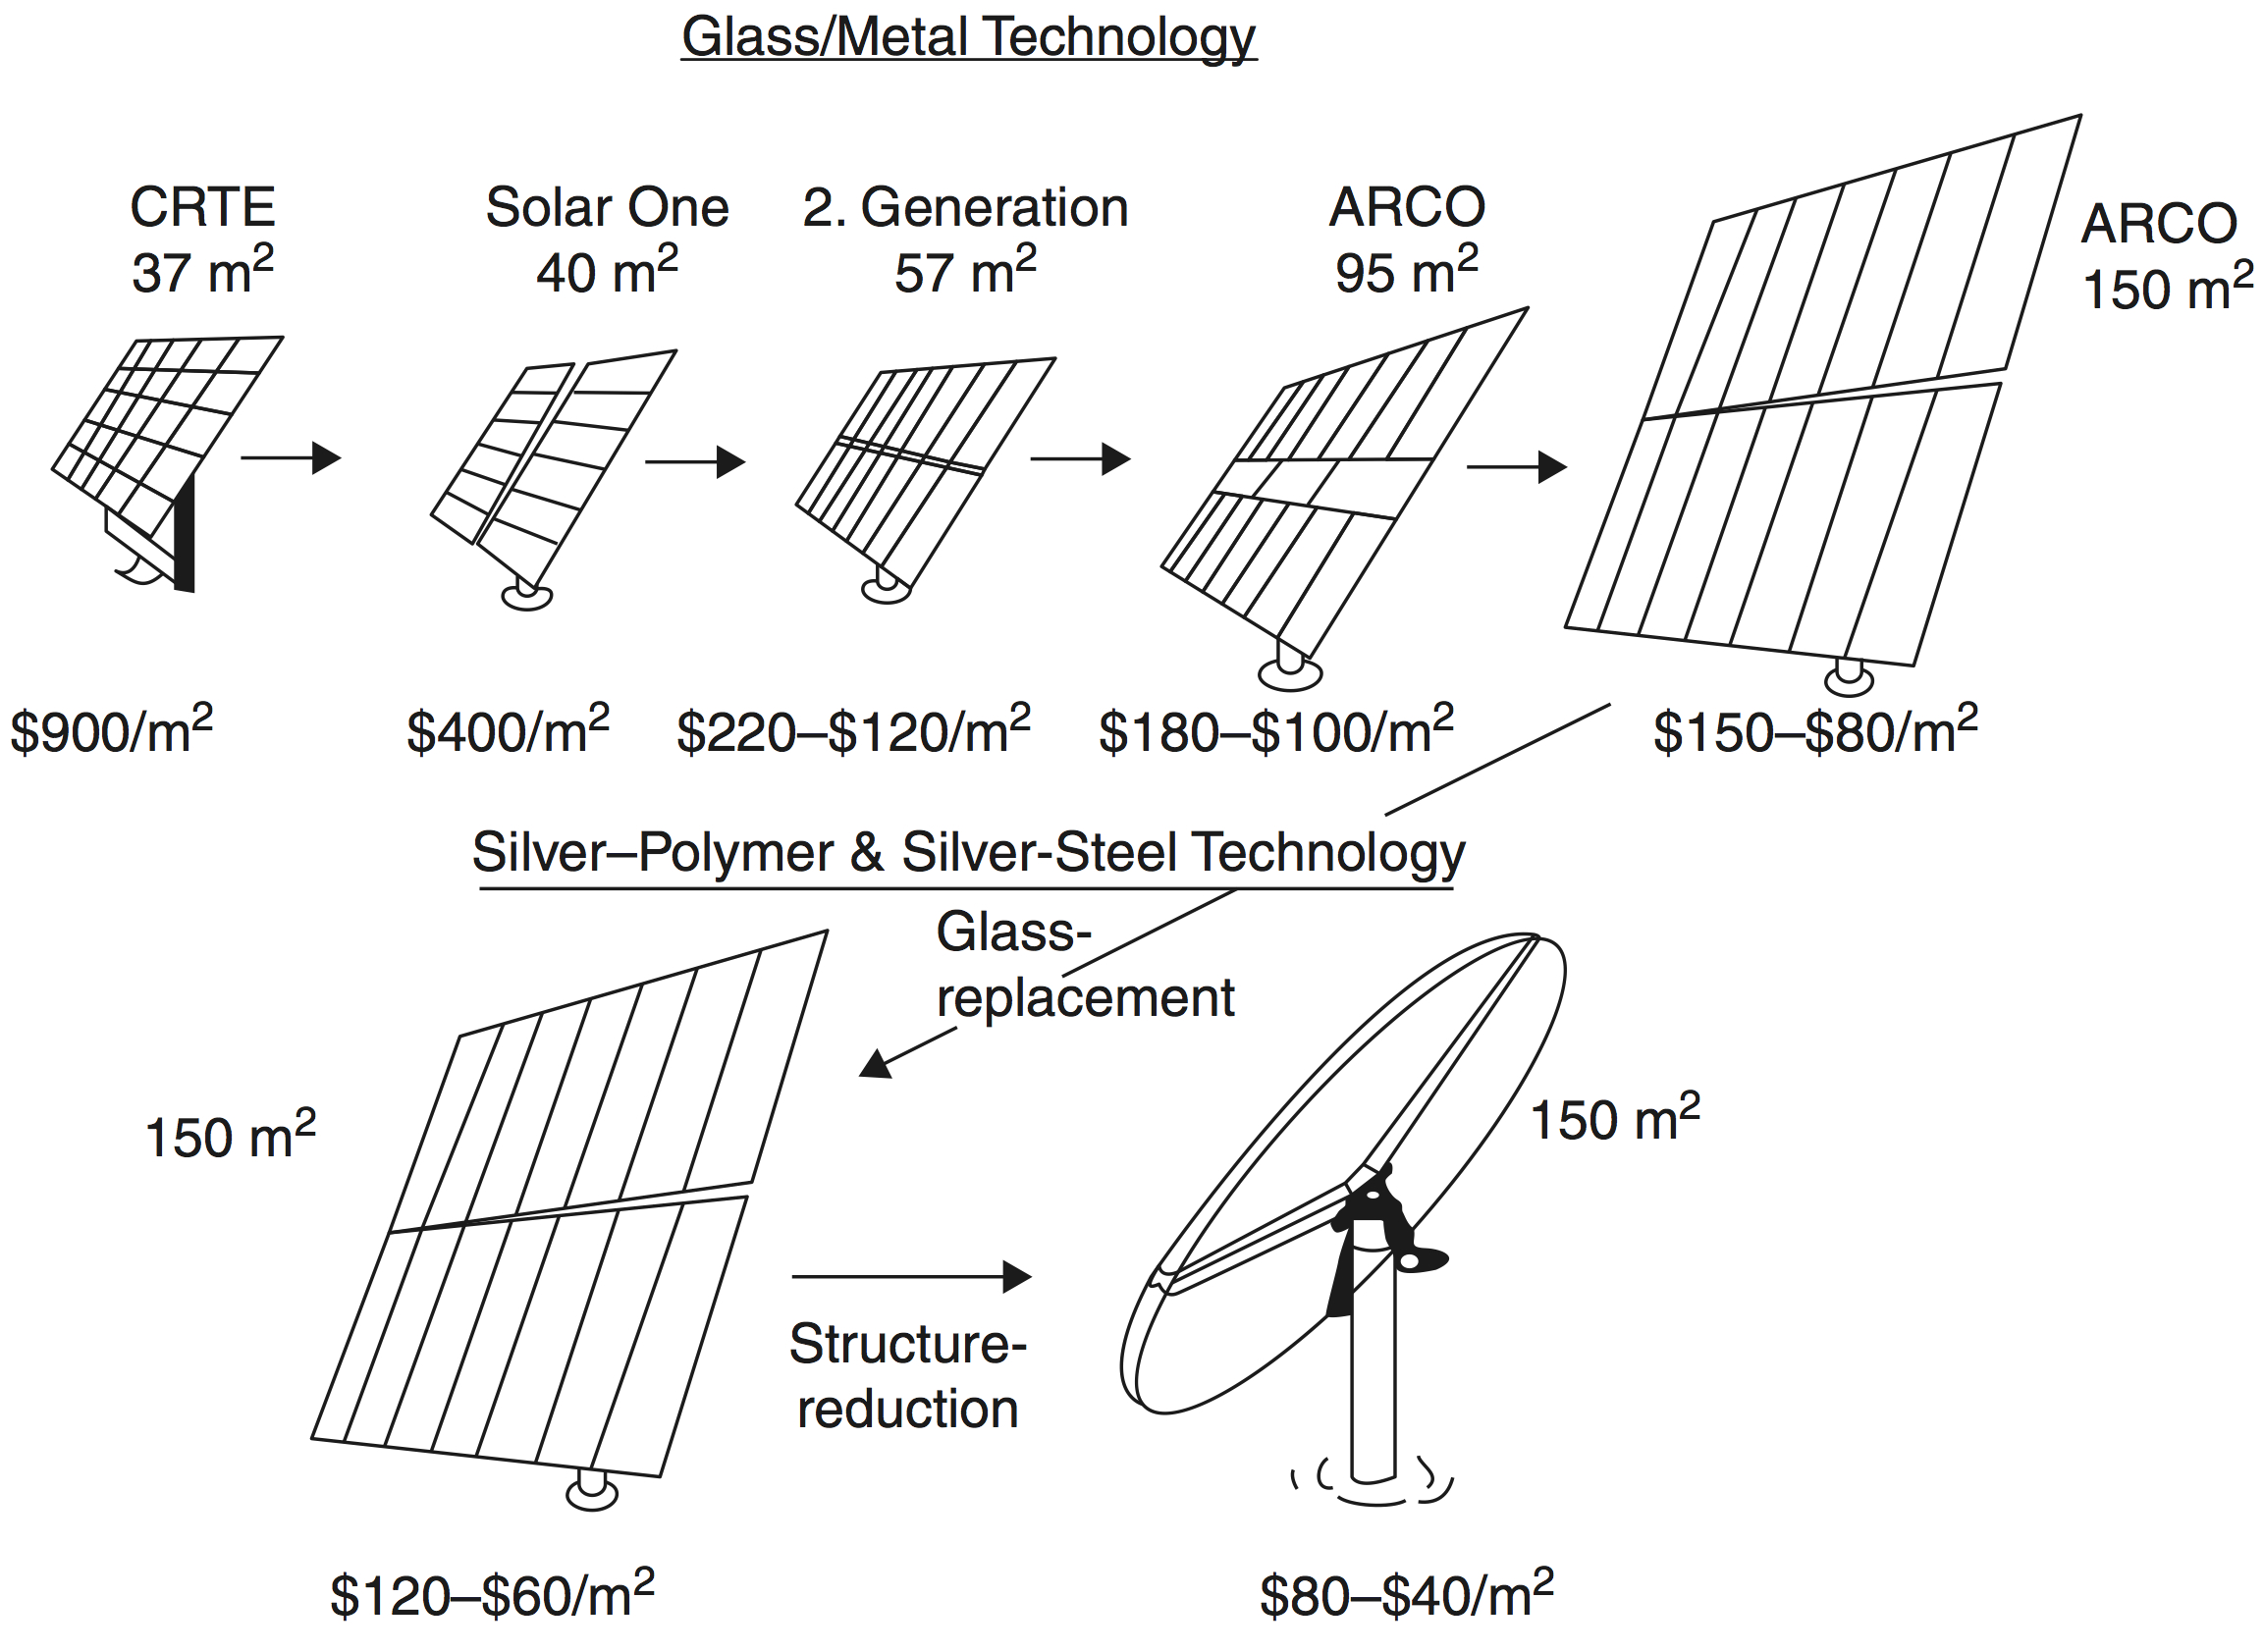
\includegraphics[width=0.9\linewidth]{FIG/Heliostats}
\caption[Heliostats used in solar power plants and their costs.]{Heliostats used in solar power plants and their costs \cite{Kolb2007}.}\label{Heliostats}
\end{figure}
\subsubsection{Heliostat field design}
The heliostat field layout is a complex topic. Decisions regarding the best position for locating heliostats relative to the receiver and how high to place the receiver above the field constitute a multifaceted problem, in which costs and heliostat loss mechanisms are among the variables, and which is solved by an iterative process. Therefore the location and the receiver type is decisive. In the northern hemisphere, the position of the sun is to the south of the plant and the field must be placed to the north of the tower. In the southern hemisphere the opposite is true. The general terminology for this position would be the "polar side" of the tower, which can be applied to towers in both the northern and southern hemispheres. The opposite side of the tower is the
"equatorial side" \cite{Alexopoulos2013}. The basically distinguishable field design types are shown in Figure \ref{Fielddesign} and can either surround the tower (Surround-field) for larger systems or be spread out on the shadow side of the tower (Polar-field) in the case of smaller systems.
\begin{figure}[!htbp]
        \centering
        \begin{subfigure}[b]{0.5\textwidth}
                \centering
                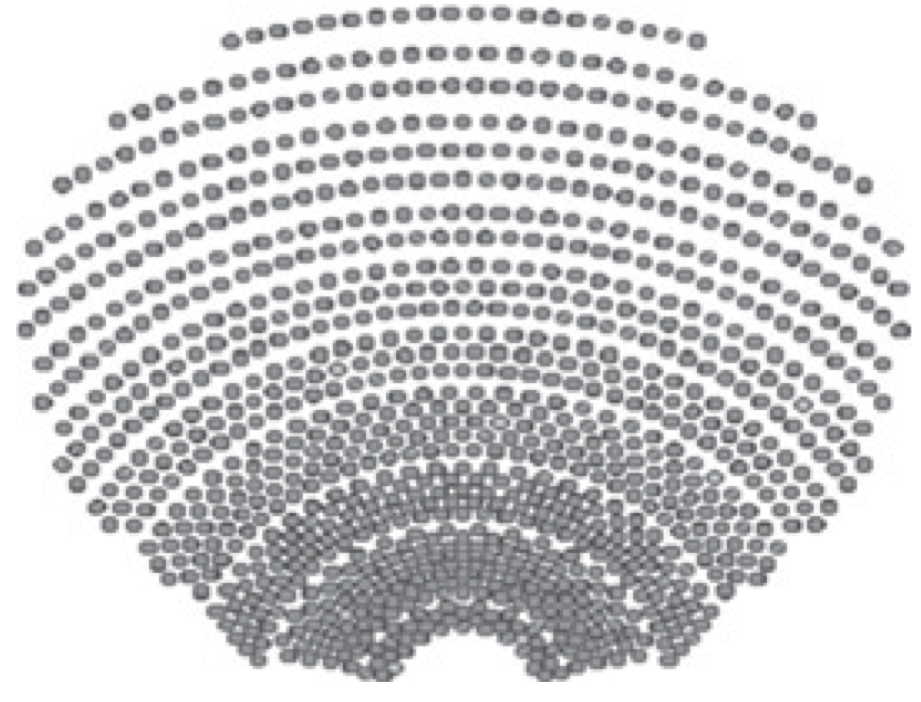
\includegraphics[width=0.9\textwidth]{FIG/north_field_layout}
                \caption{Polar-field layout.}\label{north_field_layout}
        \end{subfigure}%
        ~
        \begin{subfigure}[b]{0.5\textwidth}
                \centering
                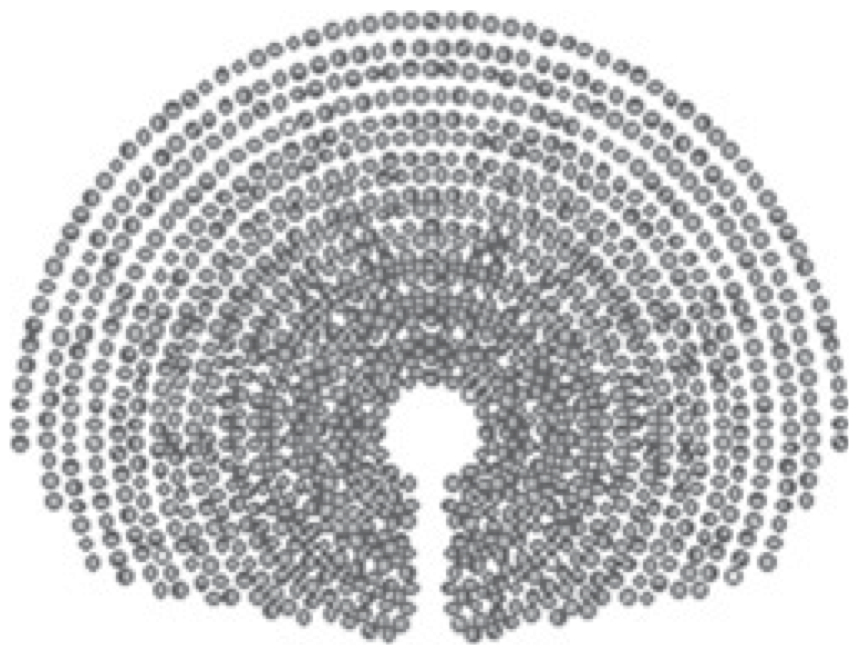
\includegraphics[width=0.9\textwidth]{FIG/sourround_field_layout}
                \caption{Surround-field layout.}\label{sourround_field_layout}
        \end{subfigure}
        \caption[Basically distinguishable field design types.]{Basically distinguishable field design types \cite{Kulichenko2012}.}\label{Fielddesign}
\end{figure}
With a field on only one side of the tower, a cavity receiver is usually used. Close to the equator, where the sun passes directly overhead, a surrounding-field can be used in combination with an open receiver (Tube receiver, see below). Another possibility is the use of two ore three fields – one on either side of the tower, in combination with a cavity receiver for each side (see Figure \ref{KhiSolarOneReceiver}). With higher power levels, surround field layouts are usually more economical. The higher the site latitude of a plant (i.e., the further away from the equator), the more the heliostat field tends to be shifted polewards. When laying out a heliostat field there are several types of losses that must be considered. These are not only the optical losses, so called, the cosine losses and losses due to shadowing, blocking, spillage (reflected radiation miss the receiver surface), and atmospheric attenuation, but also technical considerations, that is, the mirror reflectivity, mirror surface defects, tracking accuracy, wind load, and tower oscillations (due to wind load) as well as the heliostat fault rate. The aim in the designing of a heliostat field is to reliably produce the power required by the power block whilst keeping land usage and total costs to a minimum. \cite{Vant-Hull2012} \pagebreak
\subsubsection{Tower and receiver}
The function of the tower is to positioning the receiver in the required height above the heliostat field. So the choice of tower constructions depends primarily on the required height of the tower. But the height of the tower is limited by its cost. Towers are mainly constructed of steel or reinforced concrete. 



The function of a receiver is to absorb the concentrated solar irradiation energy impinging from the heliostat field and transfer it to the working fluid. Requirements to a solar receiver include high thermal conductivity, dark color of the body for high absorptivity, and temperature resistance. According to Prof. Dr. Hoffschmidt \cite{Hoffschmidt2014} from the German aerospace center (DLR) there are actually two main receiver types state of art for CR power plants, which uses molten salt and water for direct steam generation: external (tube) receiver and cavity receiver. 
\begin{figure}[!htbp]
        \centering
        \begin{subfigure}[b]{0.5\textwidth}
                \centering
                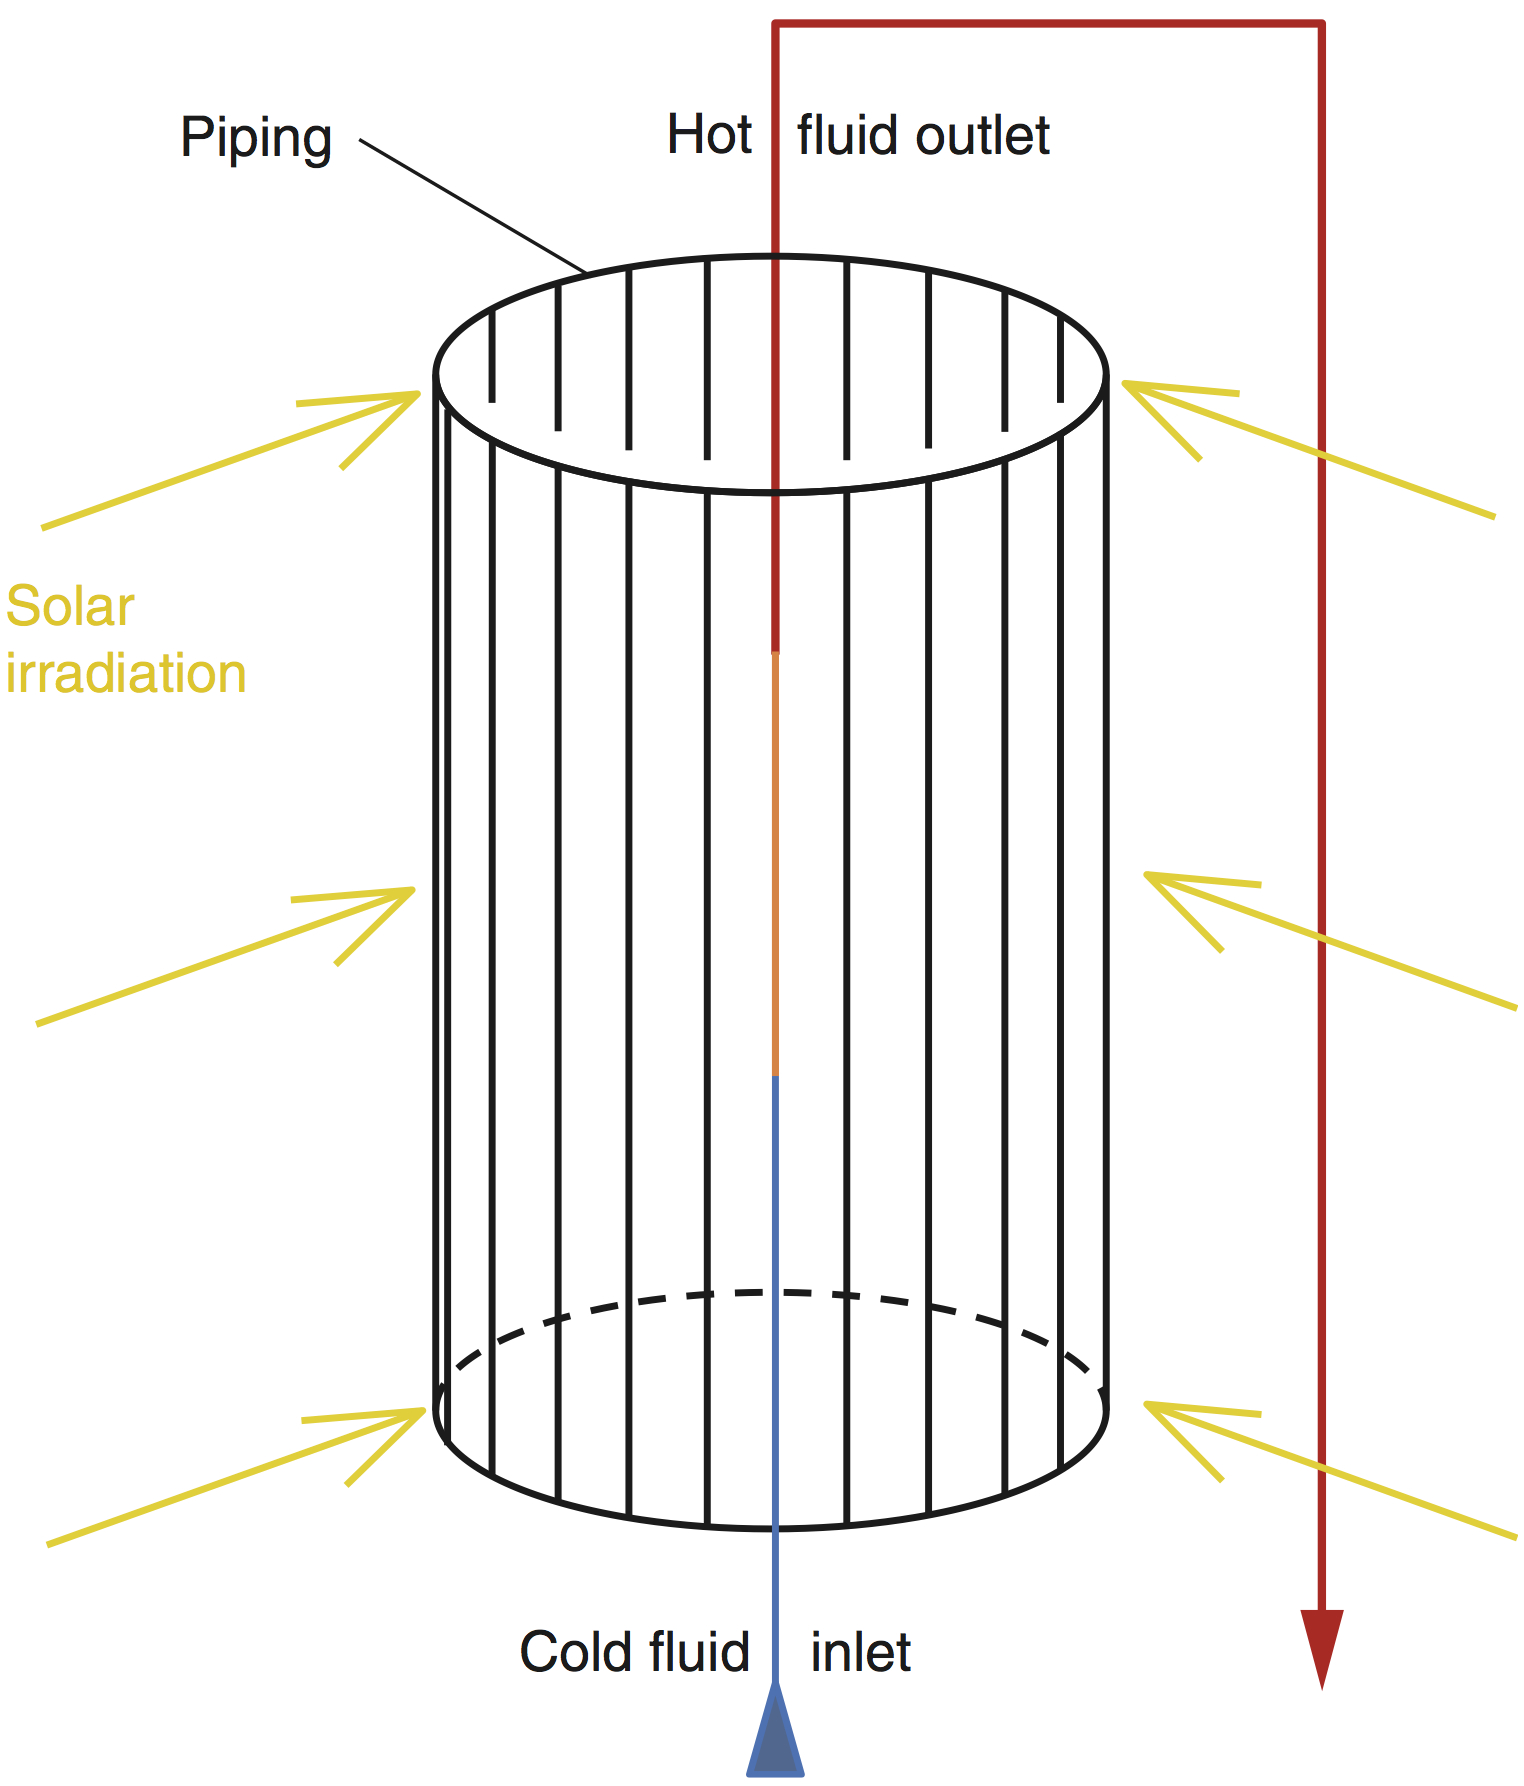
\includegraphics[width=0.9\textwidth]{FIG/TubeReceiver}
                \caption{External tube receiver concept \cite{Alexopoulos2013}.}\label{TubeReceiver}
        \end{subfigure}%
        ~
        \begin{subfigure}[b]{0.5\textwidth}
                \centering
                \includegraphics[width=0.9\textwidth]{FIG/Gemasolar_tower_heatshield}
                \caption{External tube receiver implemented in Gemasolar power plant \cite{Microtherm2012}.}\label{Gemasolar_tower_heatshield}
        \end{subfigure}
        \caption[External tube receiver concept and example of application.]{External tube receiver concept and example of application.}\label{TubeReceiverConceptGemasolar}
\end{figure}


An external receiver consists a large number of vertically arranged pipes or flat plates through which the HTF is pumped in upward direction. There are variations of shapes for the external receiver, mostly cylindrical or square-shaped. The tubes in the receiver can be crosswise arranged with different zones for pre-heating, evaporation and superheating (in case of super heated steam). Typical solar heat fluxes in this type of receiver are up to 1 MW/m$^2$ \cite{Pitz-Paal.2013}. An basic concept for an external receiver is shown in Figure \ref{TubeReceiver} with a cylindrical shape. An example for such a external tube receiver is the receiver of the Gemasolar power plant, that used molten salt as HTF. The receiver consists of a great number of HTF pipes. The external receiver pipes are fixed vertically whereby the salt smelt is pumped in upward direction. The receiver outlet temperature of the molten salt is approximately 565$\,^{\circ}\mathrm{C}$. The tube receiver of the Gemasolar power plant is shown in Figure \ref{Gemasolar_tower_heatshield}. An other example  is the Ivanpah Solar Electric Generating System (ISEGS) in California’s Mojave Desert where they produce direct steam at 550$\,^{\circ}\mathrm{C}$ using an external tube receiver which is square-shaped. A disadvantage for using the pipe receiver is the high reflection loss which is higher than for other receiver types. One way to reach reduction of thermal losses is an cavity arrangement and a face down arrangement. \cite{Hoffschmidt2014}
\begin{figure}[!htbp]
        \centering
        \begin{subfigure}[b]{0.5\textwidth}
                \centering
                \includegraphics[width=0.9\textwidth]{FIG/CavityReceiver}
                \caption{Basic cavity receiver concept \cite{Alexopoulos2013}.}\label{CavityReceiver}
        \end{subfigure}%
        ~
        \begin{subfigure}[b]{0.5\textwidth}
                \centering
                \includegraphics[width=0.9\textwidth]{FIG/KhiSolarOneReceiver}
                \caption{Three under construction situated cavity receiver mounted at the  Khi Solar One Tower \cite{CMI_Energy2015}.}\label{KhiSolarOneReceiver}
        \end{subfigure}
        \caption[Cacity receiver concept and example of application.]{Cavity receiver concept and example of application.}\label{CavityReceiverConceptKhiSolar}
\end{figure}


A cavity receiver consists of a cavity with a small opening where the receiver is located. The concentrated solar irradiation is directed into the small opening where it impinges on tubes carrying the working fluid. The idea of the cavity receiver is the reduction of thermal and optical losses. From the radiation entering the inlet aperture, only small amounts are reflected back into the atmosphere through the inlet aperture. Figure \ref{CavityReceiver} shows the basic concept of an cavity receiver. The cavity receiver concept is implemented in the PS10 solar tower plant in Spain. The direct irradiated absorber tubes is basically a forced circulation radiant boiler with low ratio of steam at the panels output, which produce saturated steam at 250$\,^{\circ}\mathrm{C}$ and 40~bar. A schematic diagram of the PS10 is shown in Figure \ref{directsteamgeneration}. SA first solar power tower will also use a cavity receiver technology. Figure \ref{KhiSolarOneReceiver} shows the three under construction situated cavity receiver of the Khi Solar One. Two steam generator (east and west orientated) and one super heater (south orientated) using the cavity receiver concept are external mounted on the tower \cite{Prof.Dinter2015}.
\subsubsection{Current stage of commercial scale CR power plants}
As shown above there is a variety of CR concepts also for commercial scale. But there are three outstanding CR projects worth mentioning for large-scale commercial application. The Khi Solar One, the Ivanpah Solar Electric Generating System (ISEGS) and the Atacama-1.



Fore SA obviously the Khi Solar One, which will be the first commercial scale CR power plant in the country. This 50.0~MW$_{el}$ power tower is under construction and will be operated by Abengoa Solar. The Polar-field consists out of 4~120 heliostats with a reflection surface of 140.0~m$^2$ each concentrate direct solar irradiance on three cavity receiver. \cite{NREL2014,Prof.Dinter2015}



The Ivanpah Solar Electric Generating System (ISEGS) is currently the largest CSP plant operating by BrightSource. The three-unit power system with in total 377.0~MW was started operation 2014 in Ivanpah Dry Lake, California. The three external square-shaped receiver on each tower are focused by 173~500 heliostats with a aperture area of 15.0~m$^2$ each. The costs for the power plant which consists out of three CRS are approx. 2~200~USD million. But instead of an storage system BrightSource using a natural gas fired backup for the ISEGS. \cite{BrightSourceEnergy2014,NREL2014a}



One of the highly promising CR projects for large-scale commercial application is Abengoa Solars Atacama-1. The eponymous Atacama desert in Chile, where the plant is under construction, has the highest levels of solar radiation worldwide. The scheduled operation start of the plant is in 2018. 10~600~heliostats each 140~m$^2$ in aperture area will concentrate on a external cylindrical shaped receiver with 32~m in height and 19~m in diameter. The receiver will be positioned in a 243~m-tower to heat molten salt to drive a 110~MW$_{el}$ steam turbine and 17.5~h direct thermal storage. This will generate electricity 24~h per day, similar to the Gemasolar power plant, but more than five times that powerful. This project constitutes the current state of art in commercial scale CRS. \cite{NREL2015b,AbengoaSolar2015a,AbengoaSolar2015}
\pagebreak
\subsection{Heat transfer fluid} \label{subsection_HTF}
In each CSP family, various options exist for the heat transfer fluid, the storage technology, and the thermodynamic cycle. The heat transfer fluid (HTF) removes heat from the receiver and transfer it either to the storage system or to the final use. The correct choice of the fluid is determinant in order to reduce costs and increase the efficiency of the plant. The most important HTFs are:
\begin{itemize}
\item \textbf{Synthetic oils} They are used predominant in PTCs thanks to their low pumping losses, their adequate conductivity and the fact that they do not need very high pressures, around 16 bar. However, they face a temperature limit of 393$\,^{\circ}\mathrm{C}$, which limits the efficiency of the plant. In addition, they are toxic and flammable.
\item \textbf{Direct steam generation} If saturated or superheated steam is generated directly at the receiver two main advantages are found: first, no heat exchanger is required in order to generate steam from the HTF and second, the exergy loss that takes place at such heat exchanger is avoided. However, some issues are also found: high pressures are required, which makes it not suitable for PTC's due to leakages at the movable elements, different thermal regimes are found in the steam generation, which complicates transients and superheating, and no efficient method has been found for energy storage. This last point is a main issue, especially when the importance of dispatchability is considered.
\item \textbf{Molten salts} Molten salts are playing a great role in CSP for energy storage. The most commercial molten salts have a working temperature range from 290$\,^{\circ}\mathrm{C}$ to 565$\,^{\circ}\mathrm{C}$, and thus higher efficiencies are obtained at the power block (cf. Table \ref{TableSensbleHeatStorageMaterial}). However, they have the issue of solidifying at relative high temperatures. As a result, if the receiver cannot be evacuated when there is no impinging sun, which is the working mechanisms in central towers with molten salts, the fluid must be recirculated from the hot tank to the cold tank, increasing thermal energy losses. Evacuation of linear receivers seems more difficult than in central towers due to the fact that tubes are horizontal.
\item \textbf{Pressurized gasses} Gasses do not have any limit in temperature, neither by the upper nor by the bottom part. In addition, they are cheap, especially if the air is used as it is found in the atmosphere. However, pumping losses are much higher than in liquid HTFs due to the density difference. In order to overcome this issue, pressure must be increased, pumping power losses being inversely proportional to the squared power of the pressure. At current time no commercial power station uses pressurized gases, although they have been used in central tower (Solgate) and CCP research prototypes. Leakages of the gas found in the movable elements of PTCs due to the high pressures suggest the need of fixed receivers in order to use pressurized gasses.
\end{itemize}
\subsection{Storage systems for CSP}\label{Subsection_storage_system}
The storage systems plays the decisive role that makes solar thermal power stand out from other renewable energy technologies. By the integration of heat storage capacity, STP plants are actually the only operational renewable energy option on the market offering dispatchable electricity power generation in multi-MW range. With the thermal energy storage (TES) system a CSP power plant offers the advantage of an integrated solution, which does not impose additional requirement on the electrical grid. Figure~\ref{integratedstoragescheme} shows the general scheme to store thermal energy into a CSP plant. The storage unit is connected both to the solar receiver and the power block. During charging the heat (high enthalpy mass flow) from the solar receiver is transferred to the thermal cycle, while the storage unit is charged by excess thermal heat. During the discharge process, the working fluid of the power block is heated by the energy from the  storage systems. Alone or in combination with some fossil fuel backup, the storage system keeps the plant running under full-load conditions. The energy from the storage might be also used to preheat the collector system during the ramp up time of the power plant.
\begin{figure}[h] 
\centering
\includegraphics[width=0.70\linewidth]{FIG/integratedstoragescheme}
\caption[Scheme for CSP plant with integrated storage unit.]{Scheme for CSP plant with integrated storage unit \cite{Steinmann2015}.}\label{integratedstoragescheme}
\end{figure}
From a technical point of view, the storage must have high energy density, good heat transfer between the heat transfer fluid (HTF) and the storage medium, mechanically and chemically stable storage media, compatibility between the heat exchanger, heat transfer fluid and storage medium, complete reversibility, and minimum thermal losses. Actually, there are just four commercial used TES in CSP plants integrated (see below). But in generally a TES system, can store heat in the form of sensible, latent, or thermochemical energy. Latent and thermochemical based TES systems are still in the phase of research and development \cite{Steinmann2015}.
\begin{figure}[t]  
\centering
\includegraphics[width=0.75\linewidth]{FIG/Basicstorageconcepts}
\caption[Basic storage concepts for CSP systems.]{Basic storage concepts for CSP systems.}\label{Basicstorageconcepts}
\end{figure}


In Figure~\ref{Basicstorageconcepts} is on one site the more basic concepts for a direct storage shown, which use the same working fluid for the storage system and the solar receiver and on the other site indirect systems transferring energy to a separate storage medium. The various storage concepts show different states of maturity. These commercial integrated storage systems and their application range will described in the following \cite{Steinmann2015}:
\begin{itemize}
\item Direct storage of heat transfer oil (Direct Storage of Liquid Working Fluid)
\item Indirect molten salt storage units (Indirect Storage in Liquid Media)
\item Steam accumulators (Direct Storage with Phase Change)
\item Direct molten salt storage units (Direct Storage of Liquid Working Fluid)
\end{itemize}
According to the "Technology Roadmap - Energy storage" of the International Energy Agency from 2014, alternative storage concept like heat storage with phase changing materials (PCM), thermochemical energy storage, and waste heat utilisation methods offer many potential opportunities. However, these technologies will need to overcome containment vessel design and material stability challenges at very high temperatures before they can achieve widespread deployment and will not further described or disused here. \cite{IEA2014e}

Likewise alternative concepts in liquid storage media such as dual media concepts (thermocline) and floating barrier concepts are still in the phase of research and development and will not be further described.\cite{Steinmann2015} 



In the following sensible liquid media will be described. Therefor the physical principles of heat storage systems are necessary. The amount of heat, $Q$ (in J), which can be stored in liquid sensible systems and the density, $E$ (J/m$^3$), related with this process can be calculated using the following equations:
\begin{align}
Q=m*C_p*(T_{out}-T_{in})=m*C_p*\Delta T \label{GL_heat}
\end{align}
\begin{align}
E=\rho*C_p*(T_{out}-T_{in})=\rho*C_p*\Delta T \label{GL_density}
\end{align}
where $T_{in}$ and $T_{out}$ are inlet and outlet storage system temperatures, respectively [K], $m$ is mass of storage liquid media [kg], $\rho$ is density [kg/m$^3$], and $C_p$ is specific heat capacity [J/(kg*K)]. Analyzing equation \ref{GL_heat} and \ref{GL_density}, it can be concluded that an optimum liquid sensible storage material must present high heat capacity, $C_p$, and a wide range of thermal stability, $\Delta T$. Different fluids have been studied as HTF and liquid sensible storage media \cite{Gil2010} and are shown in Table \ref{TableSensbleHeatStorageMaterial}. \cite{Ushak2015}
\begin{table}[h]
\centering
\includegraphics[width=1\textwidth]{FIG/TableSensbleHeatStorageMaterial}
\caption[Main characteristics of sensible heat storage liquid materials.]{Main characteristics of sensible heat storage liquid materials \cite{Gil2010}.}\label{TableSensbleHeatStorageMaterial}
\end{table}
\subsubsection{Direct storage of heat transfer oil}
The simplest concept to implement a TES into a CSP plant is the direct storage of the working fluid which is circulated through the solar absorbers. The first commercial used parabolic trough power plant SEGS-1, built 1984 in California, uses a mineral oil as heat transfer medium in the absorbers, which heats up from 240$\,^{\circ}\mathrm{C}$ to 305$\,^{\circ}\mathrm{C}$. The heat from the terminal oil was used to generate a power of 13.8~MW through the the Steam-electric power block. Two 4~700~m$^3$ carbon steel  tanks were used to separate the cold from the hot oil. This made a thermal storage capacity of 120~MWh$_{th}$ possible and allowed the system generate electricity for three hours. The storage system of the SEGS-1 was destroyed by a fire in 1999 and was not replaced. Figure~\ref{troughdirecttwotank} shows a simplified scheme of the SEGS-1 parabolic trough plant and their direct storage of heat transfer fluid. Mineral oil is today not considered to be an attractive medium for TES in large-scale CSP applications. The capital costs for large oil volume are substantial and needs additional investments for possible environmental hazards like oil leaks. Also the maximum operational temperature fore mineral oil is below 340$\,^{\circ}\mathrm{C}$, which restricts the efficiency of the thermal process. Present solar through power plants are using a synthetic heat transfer fluid whose costs are significantly higher (cf. Table \ref{TableSensbleHeatStorageMaterial}). Also increased the maximum temperature of the heat transfer fluid to 390$\,^{\circ}\mathrm{C}$ and needs a vapor pressure up to 10~bar at these temperatures, which is not able to storage stable at these conditions. All this made the direct storage of heat transfer oil not longer to the state of the art. \cite{Richter2013}

\begin{figure}[!ht]
        \centering
        \begin{subfigure}[b]{0.5\textwidth}
                \centering
                \includegraphics[width=0.6\textwidth]{FIG/troughdirecttwotank}
                \caption{SEGS-1 PTC plant with direct storage of heat transfer fluid.}\label{troughdirecttwotank}
        \end{subfigure}%
        ~
        \begin{subfigure}[b]{0.5\textwidth}
                \centering
                \includegraphics[width=1\textwidth]{FIG/troughtindirecttwotank}
                \caption{PTC power plant with indirect storage system using molten salt.}\label{troughtindirecttwotank}
        \end{subfigure}
        \caption[Simplified scheme of PTC power plants and storage concepts.]{Simplified scheme of PTC power plants and storage concepts \cite{Steinmann2012}.}\label{storageconceptstrough}
\end{figure}
\subsubsection{Indirect molten salt storage units}
Since the direct storage of the synthetic HTF is not attractive, an indirect storage concept was proposed. This should use a low cost storage medium, which can be stored at ambient pressure between 290$\,^{\circ}\mathrm{C}$ and 390$\,^{\circ}\mathrm{C}$. The use of molten nitrate salts was a nearby solution whose elements is considered and development since the early stage of CSP technology in the 1980's. Depending on the importance of material costs and there thermal stability, an sodium-nitrate-rich (NaNO$_3$) mixture containing 60\% NaNO$_3$ and 40\% KNO$_3$ (potassium nitrate) is preferred if an large quantities is required. The maximum temperature is in range of 550-580$\,^{\circ}\mathrm{C}$ and the melting temperature is in the range of 230$\,^{\circ}\mathrm{C}$. \cite{Richter2013}

Figure \ref{troughtindirecttwotank} shows a simplified scheme to implement a indirect two tank molten salt storage concept into a parabolic trough plant. Two separate insulated cylindrical thanks made of steel and carbon are used. Each tank can contain the total molten salt volume. Due to the temperature-dependent density of molten salt, the volume of the hot fluid tank has to be 4\% lager. To prevent freezing of molten salt an electrical immersion heaters are located at the bottom of the tanks.\cite{Kelly2006}.

The Andasol-1 facility, completed 2008 in Andalusia, Spain was the first commercial CSP plant using indirect molten salt storage. This plant can be operated for 7.5~h at 50~MW$_{el}$ by thermal energy provided by an indirect two-tank molten salt storage system. The molten salt storage fluid of 28~500~tons is cycled between 385$\,^{\circ}\mathrm{C}$ and 295$\,^{\circ}\mathrm{C}$, resulting a storage capacity of 1~050~MWh$_{th}$ \cite{Relloso2009}. The storage tanks have a height of 14~m and a diameter of 36~m. The similar CSP plants Andasol-2 and Andasol-3 started operation in 2009 and 2011. \cite{SolarMillenniumAG2008,NREL2008,NREL2013a,NREL2013}

Figure \ref{SolanaStorage} shows the Solana facility located in Arizona, USA. This plant was completed in 2013 and is the the largest parabolic trough plant so far. The indirect molten salt storage system uses 12 tanks to provide 280~MW$_{el}$ for a duration of six hours. \cite{AbengoaSolar2013a}

Since 2015 SA has also their first commercial CSP plant using indirect molten salt storage technology (Figure \ref{KaXu-solar-field}). KaXu Solar One is located next to Poffader in the Northern Cape and is a parabolic trough plant with 100~MW$_{el}$ capacity and 2.5~h of thermal storage in molten salts. \cite{NREL2015c}
\begin{figure}[!bhtp]  
\centering
\includegraphics[width=0.9\linewidth]{FIG/SolanaStorage}
\caption[Overall view of Solana PTC facility with 12 storage tanks for molten salt.]{Overall view of Solana PTC facility with 12 storage tanks for molten salt \cite{AbengoaSolar2013}.}\label{SolanaStorage}
\end{figure}
\subsubsection{Steam accumulators}
In 2007 the first commercial CSP plant in Europe, the Planta Solar 10 (PS10) started near to Seville in Spain. The power tower uses saturated steam at 250$\,^{\circ}\mathrm{C}$ and 40~bar to drive a 11~MW$_{el}$ power circle. A schematic diagram of the PS10 is shown in Figure \ref{directsteamgeneration} on Page \pageref{directsteamgeneration}. The energy availability for storage is limited because the  plant is designed for a small solar multiple value of 1.3. Therefore a stream accumulator was selected as storage concept. The cross-sectional view of an steam accumulator is shown in Figure \ref{SteamAccumulatot}, which is also denoted as Ruths' storage or saturated steam storage. During charging the surplus stream is fed into a pressurized liquid water volume. The liquid water acts as storage medium. So the condensing steam increases the pressure and temperature of the liquid water in the volume. The storage is designed in horizontal cylindrical pressure vessel, whose volume is filled with 90\% saturated liquid and the remaining volume is filled by saturated stream. Saturated stream will provided during discharge by the steam accumulator. While the saturated steam is taken out of the steam accumulator is the pressure in the liquid volume declining. The saturated liquid volume generates thereby additional saturated steam by a reaction of the pressure reduction. Meanwhile the mass reduction of the liquid volume is usually in the range of 10-20\%. Pressure and temperature of the steam from the steam accumulator decline continuously during the discharge process. The PS-10 plant uses four separate tanks to store about 20~MWh$_{th}$ which is sufficient to produce 50\% load for 50 minutes. Attractive features of steam accumulators are their robustness and the simplicity of the concept. The fast reaction time makes the steam accumulator to an prefer storage concept of buffer storage solution intended for short fluctuation of solar radiation. But significant exergy losses occur due to the temperature difference between the steam and liquid volume during the charging. While steam accumulators are an attractive solution for small and medium sized solar process heat application, W.-D. Steinmann from the German Aerospace Center (DLR) \cite{Steinmann2015} has the opinion they are not expected to play a major role in the future of CSP applications. \cite{Richter2013}

Nonetheless the first power tower in SA, Khi Solar One will use super-heated steam, dry cooling technology, and a 2~h steam storage system. Khi Solar One is a 50 MW solar power tower plant being built by Abengoa near the town of Upington in the Northern Cape Province. Operation was scheduled to begin in 2014 but is still under construction (Status Oct. 2015). \cite{Abengoa2014,NREL2014}

\begin{figure}[!htbp]  
\centering
\includegraphics[width=0.7\linewidth]{FIG/SteamAccumulatot}
\caption[Scheme of a steam accumulator.]{Scheme of a steam accumulator \cite{Steinmann2006}.}\label{SteamAccumulatot}
\end{figure}
\subsubsection{Direct molten salt storage units}
Increasing the maximum process temperature of the thermal cycle of an CSP plant seams to be an efficient way to improve the economics of solar thermal electricity generation. A higher maximum process temperature allows also to increase the thermal storage cycle temperature, which has an significant impact on the specific storage capacity for sensible heat. Thereby the required storage inventory and the volume of the storage tanks can be reduced. Also less electric power for pumping the storage medium is required. But on the other hand, increasing with the higher temperature as well corrosion problems and thermomechanical stress.
\begin{figure}[t!]  
\centering
\includegraphics[width=0.45\linewidth]{FIG/towerdirecttwotank}
\caption[Simplified scheme of Solar Two CRS power plant with direct storage of molten salt used as heat transfer fluid.]{Simplified scheme of Solar Two CRS power plant with direct storage of molten salt used as heat transfer fluid \cite{Richter2013}.}\label{towerdirecttwotank}
\end{figure}


Using the solar central receiver concept is an opportunity to raise the temperature of the process up to more than 565$\,^{\circ}\mathrm{C}$. Figure \ref{towerdirecttwotank}  shows a simplified scheme of direct two-tank molten salt storage concept integrated into CRS. This concept was first tested in the Solar Two power plant. This pilot solar-thermal project was built in the Mojave Desert just east of Barstow, CA, USA in 1994 on basis of the Solar One facility and was operating until 1999. A 10~MW$_{el}$ Rankine cycle was connected to the central receiver providing 35~MW$_{th}$. The two-tank storage system had an inventory of 1~400~t of a mixture of molten sodium nitrate (60\% by weight) and potassium nitrate (40\% by weight), with a total volume of about 1~700~m$^3$. The capacity of the storage system was 107~MWh$_{th}$ and operated between 565$\,^{\circ}\mathrm{C}$ and 290$\,^{\circ}\mathrm{C}$, which allowed the operation of the turbine for 3~h. The external isolated tanks had both a diameter of 11.6~m, the hot tank was mad of stainless steel had a height of 8.4~m with thermal loss in the range of 100~kW, the cold tank made of carbon steel was 7.8~m tall and transferred about 50~kW to the environment. The Solar Two project also gained the operational experience for handling larger quantities of nitrate salt for storage applications. Although, their was some changes observed in the physical properties of molten salt during the duration of the project, their was no problems resulted. After the 30~000~h project test and the analyses of the construction material, it was concluded that salt-induced no practical limitation on the useful life of tanks. Also the nitrate salt was recycled for use as fertilizer at the end of the project. \cite{Steinmann2015} 

The first commercial solar tower plant using molten salt with a direct storage system is Gemasolar, which was commissioned in 2011. It uses the first high-temperature solar receiver with molten salt, which provides 15 hours of thermal storage and an annual capacity factor of about 75\%. The size of the storage allows the plant to operate 24~h per day. The facility generates 19.9~MW$_{el}$ from 2~650~heliostats each 120~m$^2$ aperture area. The technology is based on the Solar Two and has the same temperature difference in the receiver from 275~K. \cite{NREL2011}

The Atacama-1, which is currently under construction in the Atacama desert in Chile, will also use a direct storage in molten salt for 17.5~h of storage. \cite{NREL2015b,AbengoaSolar2015a,AbengoaSolar2015}

Also parabolic trough power plants using direct molten salt storage units. The commercial used Archimede solar power plant in Italy is the first parabolic trough plant using molten salt as HTF. It started 2010 the production with 5~MW turbine capacity. The storage capacity reaches for 8 hours and has a total mass of 1~580~t of molten salt. With a tank size of 6.5~m in height and 13.5 m in diameter, the capacity is 100~MWh$_{th}$. \cite{NREL2012}



In a nutshell, the direct or indirect two-tank molten salt storage technologies are represent current state of art for commercial large-scale CSP applications. While this concepts shows a low technical and environmental risk, the potential for cost reduction is limited here. 
\subsection{Power cycles for CSP systems} \label{subsection_powerblock}
As mentioned in the overview of solar power technologies in Figure \ref{OverviewSTP} on Page \pageref{OverviewSTP}, a range of different solar to electric energy conversion systems can be applied. Commonly used as conversion systems in current large-scale CR and PTC applications are steam turbines which are based on the Rankine cycle. Nearly all convectional fired power plants using the Rankine cycle to convert heat in electricity. If an conventional fired combined cycle power plant is supplemented with a CSP system it uses an integrated solar combined cycle (ISCC), which is also based on the Rankine cycle. An additional conversion systems for CRS and parabolic dishes is the Brayton cycle (also known as Joule cycle). However, for efficient cycle operation temperatures of 1~000$\,^{\circ}\mathrm{C}$ are needed. Therefore the Brayton cycle has just been operated in demonstration CSP systems. CSP systems also uses Organic Rankine cycles, Stirling engines and other opportunities to generate electricity. \cite{Lovegrove2012}



A CSP plant with Rankine cycle is basically working in four steps using a steam turbine:
\begin{itemize}
\item Compressing pure feed water to high pressure. 
\item Pre-heating, boiling and superheating steam in a boiler which may be in the focal point, or may be heated using a heat exchanger with another HTF. 
\item Expanding the steam to low pressure via a series of turbines that drive a generator.
\item At the end of the expansion process, condensing the low pressure steam, with the aid of a cooling tower and then re-using it in the cycle.
\end{itemize}
\newpage
\section{Large scale PV power plants}\label{Large scale photo voltaic (PV) power plants}
two axis tracking PV
\subsection{Large-scale PV power plants}

\subsection{Large-scale electrical energy storage systems}
electrical energy storage (EES)
EESSchema
\begin{figure}[htbp]  
\centering
\includegraphics[width=0.65\linewidth]{FIG/EESSchema}
\caption[Schema of an electrical energy storage (EES) system and there energy losses.]{Schema of an electrical energy storage (EES) system and there energy losses.}\label{TCC_EES}
\end{figure}

\begin{equation}
\textrm{Overall storage efficiency (AC-to-AC)} =\frac{E_{out} \textrm{ (kWh)} }{E_{in} \textrm{ (kWh)}}
\end{equation}

\begin{figure}[htbp]  
\centering
\includegraphics[width=0.75\linewidth]{FIG/TCC_EES}
\caption[Total capital cost in Euro (€) of large-scale EES systems per unit of nominal power rating including costs of power electronics, storage part, fixed obtain and maintainence and maybe incidental replacement costs.]{Total capital cost in Euro (€) of large-scale EES systems per unit of nominal power rating including costs of power electronics, storage part, fixed obtain and maintainence and maybe incidental replacement costs \cite{Zakeri2015}.}\label{TCC_EES}
\end{figure}

\section{Environmental impacts of CSP and PV}
Co2

Water use in O \& M

land use

energy use in operation and building
\cite{EASAC2011}

\cite{Caldes2012} 

\section{Chapter summary}

%\chapter{Simulation-based comparison of solar powered power plants}
To compare CSP and PV technologies, a simulated case study was performed on the basis of a CR system and PTC system. 
%Special attention was paid in this comparison for a high run time of the system during the day and the covering of a prescribed demand curve.
Specific attention was given to maximizing daytime operation and meeting the demand curve. 
% For this comparison the PV system was expanded with an electrical energy storage.
The photovoltaic system was extended with battery storage. 
% For the simulation an battery storage was selected.
% The dimension of the stored energy in this simulation went much beyond the actual technical capacity of individual electrical storage units and reaches more than one-sixt of the actual world battery storage capacity 690~GW \cite{IEA2015}.
The storage capacity allocated for the simulation considerably exceeds the real capacity of electrical storage units currently available and is more than one-sixth the globally installed battery storage capacity of 690 GW.\cite{IEA2015}
 %Therefor must be said at this point that this is a theoretical comparison from the viewpoint of the PV, in particular for this plant and storage scale.
Due to the scale and particularly with respect to the photovoltaic plant, the comparison is theoretical in nature.
\pagebreak
\section{General assumptions}
With the aim of producing quantifiable and comparable results, the different solar supplied power plants will be simulated under different input  parameters. After that, selected comparable output parameters will be analyzed, evaluated and rated.

The plant technologies selected for comparison are: 
\begin{itemize}
\item CSP molten salt central receiver with thermal energy storage
\item CSP synthetic oil parabolic trough with thermal energy storage
\item PV fixed elevated flat plate collectors with adapted electrical energy storage
\end{itemize}
The PV plant has been extended with a lithium-ion battery storage for the simulation, while the thermal energy storage of the CSP plant uses molten salt technology.
%All power plants got laid out for a maximum power output of 100~MW$_{el}$.
All plants were laid out for a maximum power output of 100 MW$_{el}$.
% For the comparison the power plants are forced to cover a selected load scenario.
The plants are driven to match a selected load scenario.
% In order to find an individual suitable power plant design to cover the scheduled output of the scenario, different layout conditions, using various storage and collecting field sizes, was tried.
In order to find an appropriate power plant design to match the load of the scenario, different layout parameters, using various storage and collecting field sizes, were tested.
% The scenario and there goals are discussed and defined in Section~\ref{Overall simulated configuration}. The location and related weather data is defined in Section~\ref{Location and weather data}.
The scenario and requirements are defined and discussed in Section~\ref{Overall simulated configuration}. The location and related weather data are described in Section~\ref{Location and weather data}.
%The solar power plants are implemented and simulated in NREL’s System Advisor Model (SAM) version SAM 2015.6.30 r3 for OS X \cite{NREL2015}.
The solar power plants are implemented and simulated in NREL’s System Advisor Model (SAM) version SAM 2015.6.30 r3 for OS X \cite{NREL2015}. 
% SAM is designed to simulate performance and financial models of different types of renewable energies. For the simulation the performance part of the software was used. The financial analysis was made separately. 
SAM is designed to simulate performance and financial models of different types of renewable energy. For this simulation, only the performance component was used. The financial analysis was done separately. 

The financial parameters and the resulting levelized cost of electricity (LCOE) are calculated separately for all power plants in Microsoft Excel 2011 (vers. 14.5.7) for Mac, using a simplified method which is documented in Appendix~\ref{ChapterLCOE} on page \pageref{ChapterLCOE} using a lifetime of 25~years for each plant.

\subsection{Simulation scenario} \label{Overall simulated configuration}
%Power plants are forced to supply the system load/demand.
A hard requirement is that plants meet the full electrical demand in the system. Figure~\ref{LoadScenarios} shows the daily average system load/demand in South Africa for the winter and summer period.
% The profiles from both load shapes rises at approx 7:00 in the morning and has there peak demand at 20:00 during the summer period.
Both profiles feature a sharp rise at approx 7:00 and have their peak demand at 20:00 during the summer period.
In winter, there is an initial peak at 9:00 and a second at 19:00.
%In order to supply this system load the simulated solar power plants are forced to generate full power output of 100~MW from 7:00 to 22:00. When the system demand comes down during the night also the power plants reduce there output from 22:00 to 7:00 to 50~MW. The scenario is called "night-reduction".
In order to match this system load, the simulated solar power plants must operate at full power output of 100~MW from 7:00 to 22:00. When the system demand drops during the night, the plants reduce there output from 22:00 to 7:00 to 50~MW. The scenario is called "night reduction".
\begin{figure}[htbp]  
\centering
\includegraphics[width=1\linewidth]{FIG/LoadScenarios}
\caption[South Africa daily average system load/demand for summer and winter days, with scheduled power production curve.]{South Africa daily average system load/demand for summer and winter days, with scheduled power production curve.}\label{LoadScenarios}
\end{figure}
%For the comparison the power plants there system design is forced to cover 90~\% of the scheduled electricity production over the first year.  Usually, in feed-in contracts the power output is fixed at specified values. The overproduction is not content of these contracts and is not remunerated. In order to generate exploitable and comparable results and also considering the common feed-in contracts for power plants, the hourly power production is cut to the planed values. So overproduction will not considered in the evaluation and analyses of the systems.
In this comparison, the system design must handle 90~\% of the scheduled electricity production over the first year. Usually, in feed-in contracts, the deliverable energy is fixed. Any overproduction is not covered by such contracts and is not remunerated. In order to generate exploitable and comparable results and considering standard feed-in contracts, the hourly power production is cut to the planned values and thus overproduction is not considered in this analysis.

%The results of the simulated scenarios and the financial analyses will be rated in two selected categories:
The results of the simulation and the financial analyses will be evaluated by the following quantitative measures:
\begin{itemize}
%\item \textbf{Load curve covering factor} [\%]: The Load curve covering factor (LCCF) describes quantitative how effective the power plant follows the required load curve of the scenarios.
\item \textbf{Load curve covering factor} [\%]: The load curve covering factor (LCCF) is an effectiveness measure describing how closely the plant follows the load curve.
%\item \textbf{Levelized cost of electricity} [\textcent /kWh]: The levelized cost of electricity (LCOE) represents the total project lifecycle costs. It is the present value of project costs expressed in cents per kilowatt-hour of electricity generated by the system over its life. \cite{NREL2015a}
\item \textbf{Levelized cost of electricity} [\textcent /kWh]: The levelized cost of electricity (LCOE) represents the total project life-cycle costs. It is the present value of project costs expressed in cents per kilowatt-hour of electricity generated by the system over its life. \cite{NREL2015a}
\end{itemize}
%There is a huge difference between the mentioned LCCF and the widespread capacity factor (CF). The CF is the ratio of the system's predicted electrical output in the first year of operation to the nameplate output, which is equivalent to the quantity of energy the system would generate if it operated at its nameplate capacity for every hour of the year \cite{NREL2015a}. As it is mentioned above is the LCCF calculated from the sum value of load covering in each hour of the year.
There is an important difference between the LCCF and the widely-used \emph{capacity factor} (CF). The CF is the ratio of the system's electrical output in the first year of operation to the nameplate output, which is equivalent to the quantity of energy the system would generate if it operated at its nameplate capacity for every hour of the year \cite{NREL2015a}. The LCCF is calculated from the sum value of load coverage in each hour of the year.

\subsection{Location and weather data} \label{Location and weather data}
%For the simulation of the solar power plants the locations and weather parameter of Upington, Northern Cape was used. This location is situated in a region with one of the highest irradiation values of the country, but also has a good water access by the Orange River. This locations was mentioned before in Chapter~\ref{Solar power in South Africa} and is marked in the GHI- and DNI-maps of SA in Figure \ref{irradiation} on Page \pageref{irradiation}.
In this simulation, locations and weather data for Upington, Northern Cape were used. This region has among the highest irradiation values in the country, but also has good water access due to the Orange River. This location was mentioned before in Chapter~\ref{Solar power in South Africa} and is marked in the GHI- and DNI-maps of SA in Figure \ref{irradiation} on Page \pageref{irradiation}. 
 
\begin{table}[!h]  
  \centering
	\begin{tabular}{  p{4.0cm}  C{4.0cm}  C{3.0cm} } 

	\hline	
\textbf{Item}  & \textbf{Value} & \textbf{Unit} \\ \hline \hline
Location & Upington & -\\ 
Station ID &  684240& -  \\ 
Data source & White Box Technologies, Inc. (31.05.2015) & -\\ \hline
Latitude & -28.40 &$\,^{\circ}$N \\ 
Longitude &  21.27 &$\,^{\circ}$E \\ 
Elevation &  836 & m \\ 
Total GHI per year  &  2~280 & kWh/m\textsuperscript{2}\\ 
Total DNI per year &  2~621 & kWh/m\textsuperscript{2}\\ 
Total DHI per year &  516 & kWh/m\textsuperscript{2}\\ 
Mean temp. &  21 & $\,^{\circ}\mathrm{C}$\\ 
Mean wind speed & 3.3 & m/s\\ \hline
\end{tabular}
\caption[Location and characteristics for the simulation in SAM.]{Location and characteristics for the simulation in SAM.}\label{tbl: Location}
\end{table}


%The input weather data for the simulation with SAM are in the EPW-format (EnergyPlus Weather Data) and produced by White Box Technologies, Inc. \cite{WhiteBoxTechnologies2015}. The EPW-files are data sets of hourly values of solar radiation and meteorological elements for a typical one-year period. This includes air temperature, dew point temperature, relative Humidity, atmospheric pressure, global horizontal solar radiation, diffuse Horizontal solar radiation, direct normal radiation, wind Speed, wind Direction and cloud cover. The for the simulation most relevant values are summarized in Table \ref{tbl: Location}. The hourly values of global horizontal and direct normal irradiance from the EPW-file is shown in Figure~\ref{Upington_GHI/DNI}. The highest irradiance value during the summer time is 1~199~Wh/m\textsuperscript{2} for GHI and 1~154~Wh/m\textsuperscript{2} for DNI. At the shortest day the highest irradiance is 625~Wh/m\textsuperscript{2} for GHI and 820~Wh/m\textsuperscript{2} for DNI.
The weather data for the simulation in SAM are in EPW format (EnergyPlus Weather Data) and produced by White Box Technologies, Inc. \cite{WhiteBoxTechnologies2015}. The EPW files are data sets of hourly values of solar radiation and meteorological elements for a typical one-year period. These include air temperature, dew point temperature, relative humidity, atmospheric pressure, global horizontal solar radiation, diffuse horizontal solar radiation, direct normal radiation, wind speed, wind direction and cloud cover. The most relevant parameters for this simulation are summarized in Table \ref{tbl: Location}. The hourly values of global horizontal and direct normal irradiance from the EPW file are shown in Figure~\ref{Upington_GHI/DNI}. The highest irradiance value during the summer is 1~199~Wh/m\textsuperscript{2} for GHI and 1~154~Wh/m\textsuperscript{2} for DNI. At the northern solstice, the highest irradiance is 625~Wh/m\textsuperscript{2} for GHI and 820~Wh/m\textsuperscript{2} for DNI.


\begin{figure}[!htbp]
        \centering
                \begin{subfigure}[b]{1\textwidth}
                \centering
                \includegraphics[width=1\textwidth]{FIG/Upington_GHI}
                \caption{Global horizontal}\label{Upington_GHI}
        \end{subfigure}%
\par\medskip % Linebreak      
        \begin{subfigure}[b]{1\textwidth}
                \centering
                \includegraphics[width=1\textwidth]{FIG/Upington_DNI}
                \caption{Direct normal }\label{Upington_DNI}
        \end{subfigure}%

        \caption[Hourly values of irradiance over a full year from Upington used in the simulation.]{Hourly values of irradiance over a full year from Upington used in the simulation.}\label{Upington_GHI/DNI}
\end{figure}
\newpage \noindent
%Most relevant for the simulation is also the position of the sun. SAM calculates the path of the sun by the position of longitude and latitude. Figure~\ref{SunPathUpington} shows the sun path diagram of Upington. From this it appears that the longest day in Upington has 13~h and 56~minutes with a maximum sun height of 85.05$\,^{\circ}$ while the shortest day has just 10~h and 19~minutes and a maximum sun height of 35.93$\,^{\circ}$.
SAM calculates the path of the sun by the position of longitude and latitude. Figure~\ref{SunPathUpington} shows the solar path diagram at Upington. It is apparent that the longest day in Upington has a duration of 13~h and 56~minutes with a maximum sun height of 85.05$\,^{\circ}$ while the shortest day has a duration of just 10~h and 19~minutes and a maximum sun height of 35.93$\,^{\circ}$.

\begin{figure}[htbp]  
\centering
\includegraphics[width=0.95\linewidth]{FIG/SunPathUpington}
\caption[Solar path diagram for Upington.]{Solar path diagram Upington \cite{PVsystSA2015}.}\label{SunPathUpington}
\end{figure}
\pagebreak 
\section{CR power plant}
\subsection{Design  and simulation} \label{CR power plant design  and simulation}
%For the CR power plant simulation in SAM the “CSP power tower molten salt" model was used. The EPW weather file for Upington from Section~\ref{Location and weather data} was used as an input file to specify the hourly atmospheric conditions. SAM uses the following input data for the simulation:
For the CR plant simulation in SAM, the \enquote{CSP power tower molten salt} model was used. The EPW weather file for Upington from Section~\ref{Location and weather data} was used as an input file to specify the hourly atmospheric conditions. SAM uses the following input data for the simulation:
\begin{itemize}
\item Latitude ($\,^{\circ}$)
\item Longitude ($\,^{\circ}$)
\item Elevation above sea level (m)
\item DNI (W/m\textsuperscript{2})
\item Atmospheric pressure (mbar)
\item Dry bulb temperature ($\,^{\circ}\mathrm{C}$)
\item Wet bulb temperature ($\,^{\circ}\mathrm{C}$)
\item Relative humidity (\%)
\item Wind velocity (m/s)
\end{itemize}
This Chapter describes in detail the crucial inputs of the CR power plant components, namely the power cycle, heliostat field, tower and receiver and thermal energy storage (TES).

As already mentioned, financial parameters and the LCOE are calculated separately in Microsoft Excel using a simplified method which is documented in Appendix~\ref{ChapterLCOE} on Page \pageref{ChapterLCOE}.

\subsubsection{Simulated configurations}
%The simulated configurations had the goal to reach 90~\% of the scheduled production curve by using variation of solar multiple and full load hours of TES. Also the simulated configurations covers a broad view on the technology possibilities. As already mentioned in Section~\ref{Large scale concentrated solar power (CSP) plants} is the SM the ratio of the receivers thermal output to the power cycles thermal input at design point. So a CR system with a SM of 1 has a receiver and a heliostat field which provides the thermal power needed for the power block to run at full load at the system design point. A receiver and collector field with a SM of 1 don't produce enough thermal power to store energy in a TES while feeding the turbine. A CR system with a SM of 1 is just suitable for systems without TES. To covering the scheduled load the solar multiple was varied from 2 to 3.5 in steps of 0.5. Also the storage full load hours were varied from 8 to 16~h in steps of 2~h. The target of 100~MW net capacity was reached with a gross capacity of 111~MW with an estimated gross-to-net conversion factor of 0.90. Table~\ref{tbl: CR_OverallConfig} summarizes the simulated configurations.
The simulated configurations were to meet 90~\% of the scheduled production curve by using variation of solar multiples and full load hours of TES. As mentioned in Section~\ref{Large scale concentrated solar power (CSP) plants} the solar multiple (SM) is the ratio of the receiver's thermal output to the power cycles thermal input at the design point. Thus, a CR system with a SM of 1 has a receiver and a heliostat field which provides the thermal power needed for the power block to run at full load at the system design point. A receiver and collector field with an SM of 1 do not produce enough thermal power to store energy in a TES while also feeding the turbine. A CR system with a SM of 1 is just sufficient for systems without TES. In order to cover the expected load, the solar multiple was varied from 2 to 3.5 in steps of 0.5, while storage full load hours were varied from 8 to 16~h in steps of 2~h. The target of \SI{100}{MW} net capacity was reached with a gross capacity of 111~MW with an estimated gross-to-net conversion factor of 0.90. Table~\ref{tbl: CR_OverallConfig} summarizes the simulated configurations.

\begin{table}[!h]  
  \centering
	\begin{tabular}{ p{4.0cm}  C{1.0cm} C{0.3cm} C{0.3cm} C{0.3cm} C{0.3cm} C{0.3cm} | C{0.3cm} C{0.3cm} C{0.3cm} C{0.3cm} C{0.3cm} } 
	\hline	
\textbf{Item} & \textbf{Unit} & \multicolumn{10}{c}{\textbf{Value}} \\ \hline \hline
Net turbine capacity & MW\textsubscript{el} & \multicolumn{10}{c}{100} \\
Gross turbine capacity & MW\textsubscript{el} & \multicolumn{10}{c}{111} \\ \hline
Solar multiple & - & \multicolumn{5}{c}{2.0} & \multicolumn{5}{c}{2.5} \\
TES capacity & h &  8 & 10 & 12 & 14 & 16 &  8 & 10 & 12 & 14 & 16 \\ \hline 
Solar multiple & - & \multicolumn{5}{c}{3.0} & \multicolumn{5}{c}{3.5} \\
TES capacity & h &   8 & 10 & 12 & 14 & 16 &  8 & 10 & 12 & 14 & 16 \\ \hline 
\end{tabular}
\caption[Simulated CR solar multiple and thermal energy storage configurations.]{Simulated CR solar multiple and thermal energy storage  configurations.}\label{tbl: CR_OverallConfig}
\end{table}
\subsubsection{Power cycle}
The power cycle of the simulated CR system features a Rankine-cycle steam engine, two open feed-water heaters, a pre-heater, boiler and super-heater \cite{NREL2015a}. As mentioned above has the turbine a gross capacity of 111~MW\textsubscript{el} and a nameplate (net) capacity of 100 MW\textsubscript{el}. 
\begin{table}[!h]  
  \centering
	\begin{tabular}{  p{7.0cm}  C{2.0cm}  C{2.0cm} } 
	\hline	
\textbf{Item} & \textbf{Value} & \textbf{Unit} \\ \hline \hline
Turbine design capacity, gross  & 111 & MW\textsubscript{el} \\ 
Turbine design capacity, net & 100 & MW\textsubscript{el} \\ 
Boiler operating pressure & 125 & bar \\ 
Design inlet temperature & 288 & $\,^{\circ}\mathrm{C}$ \\ 
Design outlet temperature & 566 & $\,^{\circ}\mathrm{C}$ \\ 
Cycle conversion efficiency & 41.2 & \% \\ 
Steam generator design thermal power & 269.42 & MW\textsubscript{th}  \\
Power block start-up time & 0.5 & h \\ 
Minimum required start-up temperature & 500 & $\,^{\circ}\mathrm{C}$ \\
Plant availability  & 96 & \\
Condenser type & air-cooled & - \\ 
\hline
\end{tabular}
\caption[CR power block and condecer input parameter in SAM.]{CR power block and condecer input parameter in SAM.}\label{tbl: CRPowerplant}
\end{table}
The steam generator has a HTF inlet temperature of 566$\,^{\circ}\mathrm{C}$ and outlet temperature of 288$\,^{\circ}\mathrm{C}$ at design point and operates at a pressure of 125 bar. In combination with a air-cooled condenser the CR power cycle system was simulated with a cycle gross efficiency of 41.2\%. A wet-cooled condenser would reaches some higher efficiency, but because of the lack of water in the area of Upington and the requirement by the South African government for CSP plants, a air-cooled condenser was selected. The HTF inlet temperature, pressure and efficiency values where adapted for the configuration from \cite{Kolb2011a}. For starting up the system 
needs 30 minutes and a min. required temperature of 500$\,^{\circ}\mathrm{C}$. A plant availability of 96~\% was adapted from \cite{Morin2012} in order to simulate system down-times for outages or scheduled maintenance.
\subsubsection{Heliostat field}
The heliostat field design was done in SAM using its heliostat field layout optimization tool. For the design, optimization and simulation process, heliostat data from the Sanlúcar 120 heliostat was used \cite{Noone2012}. The Sanlúcar 120 is used in the Planta Solar 10 (PS10) near Seville, Spain and is the origin of Abengoas actual heliostat ASUP 140. For a simulation with the ASUP 140 no sufficient data was available. 
\begin{table}[!htbp]  
  \centering
	\begin{tabular}{ p{4.5cm}  C{1.5cm} C{1.2cm} C{1.2cm} C{1.2cm} C{1.2cm} } 
	\hline	
\textbf{Item} & \textbf{Unit} & \multicolumn{4}{c}{\textbf{Value}} \\ \hline \hline
racking & - &  \multicolumn{4}{c}{two-axis} \\
Height & m  &  \multicolumn{4}{c}{9.45} \\
Width & m  &  \multicolumn{4}{c}{12.84} \\
Reflective area & m\textsuperscript{2} &  \multicolumn{4}{c}{120.00} \\
Heliostat availability& \% &  \multicolumn{4}{c}{99} \\
Design-point DNI & W/m\textsuperscript{2} &  \multicolumn{4}{c}{950} \\
\hline
\textbf{Solar multiple}& \textbf{-} & \textbf{2.0} & \textbf{2.5} & \textbf{3.0} & \textbf{3.5}\\ \hline 
Number of heliostats & - & 9~131 & 11~530 & 13~976 & 16~658 \\
Max. distance from tower & m & 1~528 & 1~708 & 1~883 & 2010 \\
Reflective area  & ha & 109.58 & 138.36 & 167.72 & 199.90 \\
Field land area & ha & 655.59 & 821.92 & 997.95 & 1~190.99 \\ 
\hline
\end{tabular}
\caption[CR heliostat parameter.]{CR heliostat parameter.}\label{tbl: CRHeliostats}
\end{table}
The Sanlúcar 120 heliostats have an effective reflective area of 120~m\textsuperscript{2} and are tracked on 2 axes. The heliostat field layout optimization and there design depends on the turbine gross and the SM. The heliostat field was optimized therefore for all four considered configurations. SAM first generates a coarse layout and optimizes the number of heliostats and their position. The goal of the optimization is the maximum flux with minimum power constraints according to the specified design-point DNI which represents the DNI at which the power plant achieves its rated thermal capacity. Table~\ref{tbl: CRHeliostats} summarizes the heliostat datas and the values of the optimized field design for all considered solar multiples.



The optimized heliostat field layouts of the four considered SM are depict in Figure~\ref{SM}. In order to avoid mutual shading from the heliostats the heliostat density decreases with distance from the tower. The maximum heliostat distance to the tower rises with the higher SM which can be seen in the field diameter. 
\begin{figure}[!htbp]
        \centering   
        \begin{subfigure}[b]{0.5\textwidth}
                \centering
                \includegraphics[width=0.95\textwidth]{FIG/SM20}
                \caption{SM:~2.0}\label{SM2.0}
        \end{subfigure}%
        ~
        \begin{subfigure}[b]{0.5\textwidth}
                \centering
                \includegraphics[width=0.95\textwidth]{FIG/SM25}
                \caption{SM:~2.5}\label{SM2.5}
        \end{subfigure}
        
\par\medskip % Linebreak
                
        \begin{subfigure}[b]{0.5\textwidth}
                \centering
                \includegraphics[width=0.95\textwidth]{FIG/SM30}
                \caption{SM:~3.0}\label{SM3.0}
        \end{subfigure}%
        ~
        \begin{subfigure}[b]{0.5\textwidth}
                \centering
                \includegraphics[width=0.95\textwidth]{FIG/SM35}
                \caption{SM:~3.5}\label{SM3.5}
        \end{subfigure}
        \caption[Simulated heliostat field layout at diferent solar multiples (SM).]{Simulated heliostat field layout at diferent solar multiples (SM).}\label{SM}
\end{figure}
\subsubsection{Tower and receiver}
The receiver collects the concentrated irradiance from the surrounding heliostat field. The simulated receiver is build as an external cylindrical receiver and is configurated with 24 panels of thin walled (1.25 mm) receiver tubes with an outer diameter of 60 mm arranged in a circle around the tower. The receiver tubes are made from 316H stainless steel and the external surfaces of the tubes are coated with a black Pyromark paint. The paint is resistant to high temperatures and thermal cycling, and absorbed 95\% of the incident sunlight. This configuration is similar to the receiver of the  Solar Two Project accept of the outer diameter \cite{Bradshaw2002}. The panels containing molten salt (60~\% NaNO\textsubscript{3} and 40~\% KNO\textsubscript{3}) as heat transfer fluid (HTF). The receiver design inlet temperature of 288$\,^{\circ}\mathrm{C}$ and the outlet temperature of 566$\,^{\circ}\mathrm{C}$ was set before in the power block configuration. In order to achieve the desired receiver thermal power output, the height of the tower and receiver dimensions got also adjust with the optimization of the heliostat field design. The results of the optimization is shown in Table~\ref{tbl: CRSolarfield}, as well as the fixed tower and receiver parameter. The heights of the tower range from 179.77 to 236.50~m. The receiver proportions rises with the SM and the field sizes and results in a receiver thermal power range from 538.8 to 943.0 MW\textsubscript{th}.
\begin{table}[!h]  
  \centering
	\begin{tabular}{ p{5.5cm}  C{1.5cm} C{1.2cm} C{1.4cm} C{1.4cm} C{1.4cm} } 
	\hline	
\textbf{Item} & \textbf{Unit} & \multicolumn{4}{c}{\textbf{Value}} \\ \hline \hline
Receiver configuration & - &  \multicolumn{4}{c}{external cylindrical receiver}\\
Heat transfer fluid & - &  \multicolumn{4}{c}{60~\% NaNO\textsubscript{3} and 40~\% KNO\textsubscript{3}}\\
Inlet temperatures & $\,^{\circ}\mathrm{C}$  &  \multicolumn{4}{c}{288}\\
Outlet temperatures & $\,^{\circ}\mathrm{C}$  &  \multicolumn{4}{c}{566}\\
Receiver tube material & - &  \multicolumn{4}{c}{AISI316 stainless steal}\\
Receiver tube outer diameter & mm &  \multicolumn{4}{c}{60}\\
Receiver tube wall thickness & mm &  \multicolumn{4}{c}{1.25}\\
Number of panels & - &  \multicolumn{4}{c}{24}\\
Absorption factor  & - &  \multicolumn{4}{c}{0.95}\\
\hline
\textbf{Solar multiple} &  & \textbf{2.0} & \textbf{2.5} & \textbf{3.0} & \textbf{3.5}\\ \hline 
Tower height & m & 179.77 & 200.96 & 221.57 &  236.50\\
Receiver height  & m & 22.55 & 25.45 & 27.74 &  29.94\\
Receiver diameter & m & 14.85 & 16.66 & 17.91 & 18.77\\ 
Receiver aperture area & m\textsuperscript{2} & 1~052 & 1~332 & 1~561 & 1~765 \\ 
Receiver thermal power & MW\textsubscript{th} & 538.8 & 673.5 & 808.3 & 943.0 \\
\hline
\end{tabular}
\caption[CR heliostat field parameter.]{CR heliostat field parameter.}\label{tbl: CRSolarfield}
\end{table}
\subsubsection{Thermal energy storage (TES)}
The CR system was simulated using a direct two-tank molten salt thermal energy storage (TES). The storage uses directly the HTF (60~\% NaNO\textsubscript{3} and 40~\% KNO\textsubscript{3}) from the receiver as storage medium. Figure~\ref{towerdirecttwotank} on Page~\pageref{towerdirecttwotank} shows a schema of the direct storage for CR system. The design temperature of the hot storage tank (566$\,^{\circ}\mathrm{C}$) and the cold storage tank (288$\,^{\circ}\mathrm{C}$) depends also from the set value in the power block settings as before the design receiver temperatures. So the design temperature difference between the tanks is 278$\,^{\circ}\mathrm{C}$.



As defined at the begining of this Chapter, the full load hours of TES are varied in steps of 2~h from 8 to 16~h. The TES full load hours represents the time in which the storage can supply enough energy to the steam turbine and the power block to run at full design capacity. So a higher value of TES full load hours extended the time that the power plant can run during nights or cloudy days. Table~\ref{tbl: CRTES} shows that with higher TES full load hours the thermal capacity and tank volume increases as well. The simulated storage capacity is in a range of 2~155~MWh\textsubscript{th} using 8 full load hours and 4~311~MWh\textsubscript{th} using 16 full load hours. 
\begin{table}[!h]  
  \centering
	\begin{tabular}{ p{3.9cm}  C{1.0cm} C{1.2cm} C{1.2cm} C{1.2cm} C{1.2cm} C{1.2cm} } 
	\hline	
\textbf{Item} & \textbf{Unit} & \multicolumn{5}{c}{\textbf{Value}} \\ \hline \hline
Storage type & - &  \multicolumn{5}{c}{direct two-tank molten salt}\\
Storage fluid & - &  \multicolumn{5}{c}{60~\% NaNO\textsubscript{3} and 40~\% KNO\textsubscript{3}}\\
Hot tank design temp. & $\,^{\circ}\mathrm{C}$ & \multicolumn{5}{c}{566}\\
Cold tank design temp. & $\,^{\circ}\mathrm{C}$ & \multicolumn{5}{c}{288}\\
\hline
\textbf{TES full load hours} & \textbf{h} & \textbf{8} & \textbf{10} & \textbf{12} & \textbf{14} & \textbf{16}\\ \hline 
Thermal capacity & MWh\textsubscript{th} & 2~155 & 2~694 & 3~233 & 3~772 &  4~311\\
Storage volume  & m\textsuperscript{3} & 10~229 & 12~787 & 15~345 & 17~902 & 20~460\\
\hline
\end{tabular}
\caption[CR system TES parameter.]{CR system TES parameter.}\label{tbl: CRTES}
\end{table}

SAM 2015.6.30 r3 don't have a power control to follow prescribed hourly net output values. The turbine output of each day needs to be scheduled in front for the simulation. Thereby the parasitic consumer needs highly attention. Figure~\ref{CR_turbineoutput} shows the for the simulation scheduled turbine output matrix. The individual values was fixed during experimental trial. It can be seen that the turbine output is reduced to 50\% during the night as it is specified in the scenario. The power plant follows the schedule till there is no solar irradiance and no more thermal capacity in the storage left to generate power. 
\begin{figure}[htbp]  
\centering
\includegraphics[width=0.95\linewidth]{FIG/CR_turbineoutput}
\caption[TES dispatch control matrix for turbine output fraction of CR simulation in SAM.]{TES dispatch control matrix for turbine output fraction of CR simulation in SAM.}\label{CR_turbineoutput}
\end{figure}
\pagebreak
\subsubsection{Financial parameter}
The financial parameter for the LCOE calculation of the CR power plant are seperated in different specific cost parts and are sumerized in Table~\ref{tbl: CRFinance}. The method for calculating the LCOE is documented in Appendix~\ref{ChapterLCOE} on Page \pageref{ChapterLCOE} using a lifetime of 25~years and a real interest rate of 7.5~\% \cite{FraunhoferISE2013}. The interest rate could be reduced with a rising market potential.



The specific costs of the heliostat field of 180~USD/m\textsuperscript{2} coming from J. B. Blackmon \cite{Blackmon2012}. He analyzed the costs of heliostat as a function of area for a representative solar central receiver power plant and calculated the total installed costs for a field of 5~000 heliostats with 148~m\textsuperscript{2} reflective area of approximately 180~USD/m\textsuperscript{2}. The analyze results showed that the costs are increasing with the size of the heliostats from 40~m\textsuperscript{2} on. So the adopted value of 180~USD/m\textsuperscript{2} reflective area for 140~m\textsuperscript{2} heliostats can be assumed as conservative.

The remaining investment costs are based on the "Power Tower Technology Roadmap and Cost Reduction Plan" \cite{Kolb2011} from 2011.

On top of the investment costs a came 15 \% once-off surcharge for EPC and contingencies \cite{Platzer2014}.

Fichtner analyzed the annual O\&M costs with 1.84-1.96~\% of the total investment costs for CR power plants in SA \cite{Fichtner2010}. The value of 2~\% can so also be assumed as conservative.

The costs for the land purchase comes from the "African Agriculture Review" report of the Nedbank Capital, which reported the prices for farmland in SA. For the LCOE calculation of the CSP and PV system was the land purchase costs of 3~000~USD/ha assumed which is based on these report \cite{Cassell2012}.

\begin{table}[!h]  
  \centering
	\begin{tabular}{  p{5.0cm} C{2.0cm} C{1.5cm}  C{1.5cm}  C{4.0cm} } 
	\hline	
\textbf{Item} & \textbf{Symbol}& \textbf{Value} & \textbf{Unit} & \textbf{Source}\\ \hline \hline
Heliostat field &$c_{HF}$ & 180 & USD/m\textsuperscript{2} & \cite{Blackmon2012}\\ 
Power block & $c_{PB,CR}$ & 1000 & USD/kW\textsubscript{el} & \cite{Kolb2011}\\ 
Thermal energy storage&$c_{TES,CR}$ & 30 & USD/kWh\textsubscript{th}  & \cite{Kolb2011}\\ 
Tower and receiver& $c_{T+R}$& 200 & USD/kW\textsubscript{th}  & \cite{Kolb2011}\\ 
Annual O\&M & $f_{O\&M,CR}$ & 2 & \% &\cite{Fichtner2010}\\
Land purchase&$c_{LP}$ & 3~000 & USD/ha & \cite{Cassell2012}\\ \hline
Lifetime &$n$ & 25 & years & \cite{FraunhoferISE2013} \\ 
Interest rate & $i_{CR}$ & 7.5 & \% & \cite{FraunhoferISE2013} \\ 
Annual insurance costs& $f_{ins,CR}$ & 0.5 & \% & \cite{IRENA2012}\\
Surcharge for EPC, project management and risk & $f_{EPC,CR}$& 15 & \% & \cite{Platzer2014} \\
Total plant availability & $f_{avail,plant,CR}$ & 96 & \% & \cite{Morin2012} \\ 
\hline
\end{tabular}
\caption[Finacial input parameter for CR-simulation in SAM.]{Finacial input parameter for CR-simulation in SAM.}\label{tbl: CRFinance}
\end{table}
\subsection{Results of CR power plant simulation}
The following sections illustrates and discuss the obtained simulation and calculation results of the above defined CR power plant. Therefore the load curve covering performance and LCOE as well as the belonging load profiles and duration curves are described and analyzed. The configuration of the power plants to reach 90~\% of the prescribed load while using the best belonging LCOE is defined at the end of each section.
\subsubsection{Load curve covering}
To find the suitable power plant configuration of the CR system to reach the target of 90~\% load curve covering, there was 20 various configurations simulated. This section presets and compare mainly the results of the simulation with the lowest SM and hours of TES configuration (SM: 2.0 \& TES: 8~h) with the simulation using the highest SM and hours of TES configuration (SM: 3.5 \& TES: 16~h) representative for all in between. All simulated configurations are shown in Table~\ref{tbl: CR_OverallConfig} on Page~\pageref{tbl: CR_OverallConfig}.

\begin{figure}[htbp]  
\centering
\includegraphics[width=0.8\linewidth]{FIG/CR_annual_profil}
\caption[Annual average load profile of selected CR power plant configurations.]{Annual average load profile of selected CR power plant configurations.}\label{CR_annual_profil}
\end{figure}
Figure~\ref{CR_annual_profil} shows the annual load curve covering of the above mentioned CR power plant high and low configurations with the prescribed load curve. The Figure shows, that the CR power plant using a SM of 3.5 and 16~h of TES for the configuration can cover almost at any time of the year the prescribed load curve. The decreasing of the supplied electricity 8~am leads from the winter duration and will be shown in the following. The lower CR power plant configuration can just cover between 11~am and 5~pm almost the same amount electricity during the year than the high configuration. In the morning times between 6 and 7~am the energy production is coming to standstill the whole year.

At this point it might be necessary to remind, that it is just the electricity used for the annual load covering as well as for the LCOE calculation which is actually supplied at the requested time step. So the electricity which is overproduced at any time of the year is not considered. This can also be seen in Figure~\ref{CR_winter_load}. 
\begin{figure}[htbp]  
\centering
\includegraphics[width=1\linewidth]{FIG/CR_winter_load}
\caption[CR load profile during the time of winter solstice (15. June - 25. June).]{CR load profile during the time of winter solstice (15. June - 25. June).}\label{CR_winter_load}
\end{figure}
This figure shows exemplary the load curve behavior of the CR power plants during the time with the least hours of sunlight during a day of the year. The DNI is around 830~W/m\textsuperscript{2} in peak times at these days and there are also days with less or almost no direct irradiance. As mentioned, it can be seen that the net electricity production is in both cases at some times across the prescribed load curve and is not consulted further. This reaches mainly from the described dispatch control matrix from Figure~\ref{CR_turbineoutput} on Page~\pageref{CR_turbineoutput} to control the turbine output. This is not accurate at all to follow a specific load exactly during each day of the year. 

However, Figure~\ref{CR_winter_load} mainly shows the load curve behavior of the CR power plants in low and high configuration. At a SM of 2.0 with 8~h of TES the power plant can't produce enough power during the day to fill up the TES for generating power during the night. Compared to that, the CR power plant with a SM of 3.5 and 16~h of TES can almost anytime generate electricity over the whole night. But with the rising load in the morning hours the energy production stops due to the empty storage. 
\begin{figure}[htbp]  
\centering
\includegraphics[width=1\linewidth]{FIG/CR_summer_load}
\caption[CR load profile during the time of summer solstice (16. December - 26. December).]{CR load profile during the time of summer solstice (16. December - 26. December).}\label{CR_summer_load}
\end{figure}
This leads also to the above mentioned decreasing in supply at 8~am in the annual average load profile. The difference between the gross and net electricity production is coming from the parasitic consume within the power plant.

Figure~\ref{CR_summer_load} describes the load behavior of the  same power plants during the longest days of the year. It is clearly to see, that the irradiation is higher and longer during the days compare to the winter solstice. The peaks of DNI are about 1~150~W/m\textsuperscript{2} during that days. At a SM of 2.0 and 8~h of TES the CR power plant is not able to follow the prescribed electricity load over the whole day. It's coming to standstill between 6 and 7~am at least. Therefrom also the annual average load profile is coming to stand still at these time of the day. The CR power plant with a SM of 3.5 and 16~h of TES can follow the prescribed load mostly without any problems. Outstanding for the high productivity of the plant configuration is the electricity output while having low direct irradiance. At the 21. of December the plant can supply almost the whole prescribed load using reserves from the TES.

A detailed look to the parasitic behaviors of the CR power plant with a SM of 3.5 and 16~h of TES reveals a strong decreasing after a moderate increasing during the midday. This happens when the storage is full loaded and the steam turbine don't need more power. At this point a specified amount of heliostats defocusing the receiver and the power of the receivers HTF pump is getting reduced. 

\begin{figure}[!htbp]
        \centering   
        \begin{subfigure}[b]{0.65\textwidth}
                \centering
                \includegraphics[width=1\textwidth]{FIG/CR_parasitics_low}
                \caption{SM: 2.0 TES: 8 h}\label{CR_parasitics_low}
        \end{subfigure}
\par\medskip % Linebreak              
        \begin{subfigure}[b]{0.65\textwidth}
                \centering
                \includegraphics[width=1\textwidth]{FIG/CR_parasitics_high}
                \caption{SM: 3.5 TES: 16 h}\label{CR_parasitics_high}
        \end{subfigure}
        \caption[Share of annual gross energy output of selected CR power plant configurations.]{Share of annual gross energy output of selected CR power plant configurations.}\label{CR_parasitics}
\end{figure}
The parasitic load is composed from various electrical loads of the power plant, namely pumping loads, cooling loads, fixed loads and loads depending from the power generation. The share of these electrical parasitic loads and the total share of the gross energy output of the selected CR power plans can be seen in Figure~\ref{CR_parasitics}. The share of the net energy production out of the gross energy production is about 90~\%. The unused net energy output share of all simulated CR power plants is between 1.6 and 3.2~\% and went not into the LCOE calculation.

Figure~\ref{CR_parasitics_low} shows, that the net outputs share of the lowest CR power plant configuration is about 483.60~GWh.  The total sum of the annual prescribed load is 711.75~GWh. So the power plant covers the prescribed load for 67.9~\%. The net outputs share of the highest CR power plant configuration from Figure~\ref{CR_parasitics_high} is 671.69~GWh and is covering the prescribed load for 94.4~\% over the year.

Figure~\ref{CR_LCCF} summarizes the results of the load curve covering for all simulated CR configurations. The chart shows that at a SM of 2.0 all TES variations besides 8~h a covering more than 70~\% of the prescribed load. At a SM of 2.5 the and a TES about 10~h the results showed over 80~\% load covering. A load curve covering of about 90~\% is reached at a SM of 3.0 and more than 14~h of TES. The configuration with a 12~h TES reaches just 89.1~\% at a SM of 3.0. 

\begin{figure}[htbp]  
\centering
\includegraphics[width=1\linewidth]{FIG/CR_LCCF}
\caption[Load curve covering result of simulated CR systems.]{Load curve covering result of simulated CR systems.}\label{CR_LCCF}
\end{figure}
The results of the load curve covering shows that there is no appreciable difference between the 12, 14 and 16~h of TES. At a SM of 3.5 the difference is just 1.4~\% load curve covering between 12 and 16~h of TES. There is just a addition of 0.6~\% for the 8~h TES and the SM 3.0 to 3.5 configurations. 
\subsubsection{Levelized costs of electricity}
The results of the LCOE claculation for the simulated CR configurations can be seen in Figure~\ref{CR_LCOE}. They are calculated using the finacial input parameter in Table~\ref{tbl: CRFinance} and a simplified method which is documented in Appendix~\ref{ChapterLCOE} on Page \pageref{ChapterLCOE}.

\begin{figure}[htbp]  
\centering
\includegraphics[width=1\linewidth]{FIG/CR_LCOE}
\caption[LCOE calculation results for CR simulation.]{LCOE calculation results for CR simulation.}\label{CR_LCOE}
\end{figure}
The results of the calculation shows that the lowest LCOE of 137.55~USD/MWh is reached at a SM of 2.0 and 10~h of TES and is just  marginal cheaper then using 8~h of TES with a LCOE of 137.63~USD/MWh. The LCOE addition from SM 2.0 to 2.5 is goes minimal up to 138.25~USD/MWh for 10~h of TES. The highest LCOE result of the simulated configurations is 179.00~\$cent/kWh at a SM of 3.5 and 8~h of TES. 

The behavior of the 12, 14 and 16~h of TES results for all SM of the LCOE is almost identical. Just the individual value is differently.

\begin{figure}[!htbp]
        \centering                
        \begin{subfigure}[b]{0.5\textwidth}
                \centering
                \includegraphics[width=1\textwidth]{FIG/CR_LCOE_lowinvest_BreakDown}
                \caption{LCOE break-down for SM~2.0 and 8~h~TES.}\label{CR_LCOE_lowinvest_BreakDown}
        \end{subfigure}%
        ~
        \begin{subfigure}[b]{0.5\textwidth}
                \centering
                \includegraphics[width=1\textwidth]{FIG/CR_LCOE_highinvest_BreakDown}
                \caption{LCOE break-down for SM~3.5 and 16~h~TES.}\label{CR_LCOE_highinvest_BreakDown}
        \end{subfigure}
        \caption[Break-down of selected CR-LCOE calculation results.]{Break-down of selected CR-LCOE calculation results.}\label{CR_LCOE_BreakDown}
\end{figure}
The calculated LCOEs of the simulated CR power plants is composed by seven cost parts. The investment costs of power block, tower and receiver, heliostat field, land purchase, TES, additional EPC, project management (PM) and risk as well as the annual costs for operation and maintain (O\&M). The brake-down of the LCOE components can be seen in Figure~\ref{CR_LCOE_BreakDown} for the simulation of the lowest and the highest configuration.  It can be seen that the investment costs of the land purchase don't have any influence to the LCOE of the simulated CR configurations. Also the share of the EPC, PM and risk as well as the share of O\&M don't varies much.

When comprising the results of the load curve covering with the LCOE calculation the lowest LCOE for reaching the target of 90~\% is the configuration of a SM of 3.0 and 14~h of TES. The LCOE for these configuration is 149.58~USD/MWh. 

For reaching 80~\% of the prescribed load curve the lowest LCOE is 138.25~USD/MWh using a SM of 2.5 and 10~h of TES. The lowest LCOE for covering 70~\% of the prescribed load curve is also the lowest LCOE of all and is mentioned above.

\pagebreak
\section{PTC power plant}
\subsection{Design  and simulation} \label{PTC power plant design  and simulation}
The PTC power plant was simulation in the “CSP parabolic trough (physical)" model in SAM using the option "no financial model". As before the input the EPW weather file to specify the hourly atmospheric conditions from Section~\ref{Location and weather data} was used. For the PTC simulation SAM uses the following input data:
\begin{itemize}
\item Latitude ($\,^{\circ}$)
\item Longitude ($\,^{\circ}$)
\item Elevation above sea level (m)
\item DNI (W/m\textsuperscript{2})
\item Atmospheric pressure (mbar)
\item Dry bulb temperature ($\,^{\circ}\mathrm{C}$)
\item Wetbulbtemperature($\,^{\circ}\mathrm{C}$)
\item Relative humidity (\%)
\item Wind velocity (m/s)
\end{itemize}
This Chapter describes in detail the input data of the PTC power plant simulation by there components, namely the  power cycle, solar collector, solar receiver, solar field and thermal energy storage (TES).

Also for the simulation of the PTC are the financial parameters and the LCOE calculated separately Microfoft Excel using a simplified method which is documented in Appendix~\ref{ChapterLCOE} on Page \pageref{ChapterLCOE}.
\subsubsection{Simulated configurations}
In order to reaching the goal of covering 90 \% of the scheduled production curve also the simulated PTC power plant used a variation of solar multiple and full load hours of TES. To covering the scheduled load the solar multiple was varied from 2 to 5.0 in steps of 5.0. This is significantly higher SM compared the simulated CR system was necessary to reach the 90 \% covering factor. As before with the simulation of the CR, the storage full load hours were varied from 8 to 16 h in steps of 2 h. The target of 100 MW net capacity was reached with a gross capacity of 120 MW with an estimated gross-to-net conversion factor of 0.83. The comparatively high gross turbine output is nessasary for the high parasitic burden of the system. Table~\ref{tbl: PTC_OverallConfig} summarizes the simulated configurations.
\begin{table}[!h]  
  \centering
	\begin{tabular}{ p{4.0cm}  C{1.0cm}  C{0.3cm} C{0.3cm} C{0.3cm} C{0.3cm} C{0.3cm} |C{0.3cm}  C{0.3cm} C{0.3cm} C{0.3cm} C{0.3cm} } 
	\hline	
\textbf{Item} & \textbf{Unit} & \multicolumn{10}{c}{\textbf{Value}} \\ \hline \hline
Net turbine capacity & MW\textsubscript{el} & \multicolumn{10}{c}{100} \\
Gross turbine capacity & MW\textsubscript{el} & \multicolumn{10}{c}{120} \\ \hline
Solar multiple & - & \multicolumn{5}{c}{2.0} & \multicolumn{5}{c}{2.5} \\
TES capacity & h & 8 & 10 & 12 & 14 & 16 & 8 & 10 & 12 & 14 & 16 \\ \hline 
Solar multiple & - & \multicolumn{5}{c}{3.0} & \multicolumn{5}{c}{3.5} \\
TES capacity& h & 8 & 10 & 12 & 14 & 16 & 8 & 10 & 12 & 14 & 16 \\ \hline 
Solar multiple & - & \multicolumn{5}{c}{4.0} & \multicolumn{5}{c}{4.5} \\
TES capacity& h & 8 & 10 & 12 & 14 & 16 & 8 & 10 & 12 & 14 & 16 \\ \hline 
Solar multiple & - & \multicolumn{5}{c}{5.0} & \multicolumn{5}{c}{ } \\
TES capacity& h & 8 & 10 & 12 & 14 & 16 &  \multicolumn{5}{c}{ } \\ \hline 
\end{tabular}
\caption[Simulated PTC solar multiple and thermal energy storage  configurations.]{Simulated PTC solar multiple and thermal energy storage  configurations.}\label{tbl: PTC_OverallConfig}
\end{table}

\subsubsection{Power cycle}
The PTC system also uses the steam Rankine cycle technology. In the modeled cycle, feedwater is heated in open (mixed stream) feedwater heaters with two intermediate turbine extractions - once for high pressure and once for low pressure, and the steam generation equipment consists of a preheater, boiler, and superheater. The HTF temperature at the field outlet is bound primarily by HTF stability, so maximum HTF temperatures for oil troughs typically range between 370$\,^{\circ}\mathrm{C}$ and 410$\,^{\circ}\mathrm{C}$. The turbine has a gross capacity of 120~MW\textsubscript{el}. So the net turbine capacity output at design (nameplate) is 100~MW\textsubscript{el}. The design inlet temperature of the HTF in the steam generator is 393$\,^{\circ}\mathrm{C}$ and outlet temperature of 293$\,^{\circ}\mathrm{C}$ at design point and operates at a pressure of 100 bar.



Table~\ref{tbl: PTCPowerplant} shows the input parameter for the power block design in SAM. Besides the capacity of the turbine and the condecer type, the parameters are coming from \cite{Wagner2011}. It is obviously, that the cycle conversion efficiency of the PTC power plant is lower than that one from the CR power plant. This is trace back to the lower cycle temperatures and the thereby resulting lower steam pressure in the turbine.



The air-cooled condenser was selected here as well, because water is an valuable resource in the region of Upington. The cooling system is designed to covers the stem generator thermal power. 
\begin{table}[!h]  
  \centering
	\begin{tabular}{  p{7.0cm}  C{2.0cm}  C{2.0cm} } 
	\hline	
\textbf{Item} & \textbf{Value} & \textbf{Unit} \\ \hline \hline
Turbine design capacity, gross  & 110 & MW\textsubscript{el} \\ 
Turbine design capacity, net & 100 & MW\textsubscript{el} \\ 
Boiler operating pressure & 100 & bar \\ 
Design inlet temperature & 393 & $\,^{\circ}\mathrm{C}$ \\ 
Design outlet temperature & 291 & $\,^{\circ}\mathrm{C}$ \\ 
Cycle conversion efficiency & 37.74 & \% \\ 
Steam generator design thermal power & 318.0 & MW\textsubscript{th}  \\
Power block start-up time & 0.5 & h \\ 
Minimum required start-up temperature & 300 & $\,^{\circ}\mathrm{C}$ \\
Maximum turbine over design operation & 90 & \\
Condenser type & air-cooled & - \\ 
\hline
\end{tabular}
\caption[PTC power block and condecer input parameter in SAM.]{PTC power block and condecer input parameter in SAM.}\label{tbl: PTCPowerplant}
\end{table}
\subsubsection{Solar collector (SCA)}
For the simulation of the PTC system the Ultimate Trough was selected as solar collector assembly (SCA). This collector is currently not in commercial use, but comparable troughs with similar characteristics are under construction. So the Ultimate Trough can be adopted  without technical modifications and no increase of risk. Figure~\ref{PTC_Ultimate_config} shows the information of the technical input parameter for SAM. These coming directly from a publication of the developer of the Ultimate Trough, Flabeg GmbH and sbp sonne GmbH \cite{Riffelmann2014}. 
\begin{figure}[bhtp]
\centering
\includegraphics[width=0.95\linewidth]{FIG/PTC_Ultimate_config}
\caption[Screenshot of Ultimate Trough SCA input parameter for SAM.]{Screenshot of Ultimate Trough SCA input parameter for SAM.}\label{PTC_Ultimate_config}
\end{figure}
The section "Optical Calculation" shows, that the total optical efficiency at design of the Ultimate Trough is 89.9~\%. The dimensions and main characteristics of the HCE is shown in the section "Receiver Geometry".
\subsubsection{Solar receiver (HCE)}
As heat collecting element (HCE) Schott's PTR80 was selected. This receiver tube has with 0.08~m an extended tube outer diameter. Thereby the tube can contain more HTF and reduce the mass flow in the tubes. Figure~\ref{PTC_HCE} shows the for the simulation inserted parameter. The values are the results of measurements of outdoor optical efficiency and indoor receiver heat loss of parabolic trough collector from researchers of National Renewable Energy Laboratory \cite{Kutscher2012}.
\begin{figure}[htbp]  
\centering
\includegraphics[width=0.95\linewidth]{FIG/PTC_HCE}
\caption[Screenshot of Schott PTR80 input parameter for SAM.]{Screenshot of Schott PTR80 input parameter for SAM.}\label{PTC_HCE}
\end{figure}
The section "Parameter and Variations" shows the different conditions of the HCE. Variation 1 shows the optimal condition of the HCE with annulus pressure of 0.0001 torr (0.000133~hPa), so an vacuum. The estimated average heat lost is 190~W/m. This Variation counts for 98.5~\% of all HCEs. In Variation 2 the vacuum is lost and which strongly affects the heat loss. It is 1~270~W/m and counts for 1~\% of all HCEs. In Variation 3 also the protection glass is broken, so the heat loss increase to 1~500~W/m. The total weighted losses is 207.35~W/m heat loss at design and about 0.85 optical derate and is shown at the last section most below.
\subsubsection{Solar field}
PTC solar fields are separated in sections. In the simulation of the PTC system the solar field is designed in two sections. Each section carries a feed pipe and a return pipe to transport the thermal energy to the power block. Attached to the header pipes are many loops, which contains the SCAs, the HCEs and the HTF. Figure~\ref{PTC_Field_ultimate} shows an typical layout for PTC system with two field subsections. As in the Figure is the simulated PTC system designed by four SCAs per loop \cite{Riffelmann2014}.
\begin{figure}[htbp]  
\centering
\includegraphics[width=0.9\linewidth]{FIG/PTC_Field_ultimate}
\caption[Typical configuration of a solar field layout with two field subsections for a Ultimate Trough.]{Typical configuration of a solar field layout with two field subsections for a Ultimate Trough \cite{Riffelmann2014}.}\label{PTC_Field_ultimate}
\end{figure}


As mentioned before synthetic oil is used as HTF for the simulation of the PTC system. The current standard for HTF in PTC systems is Terminol VP-1. The input parameter for the HTF are shown in Figure~\ref{PTC_HTF} and are limited by the performance characteristics of Terminol VP-1 of 12 to 400$\,^{\circ}\mathrm{C}$ \cite{Therminol2015}. The velocity range of Therminol VP-1 should be in the range of 0.36 and 4.97 m/s \cite{Wagner2014} and is affected by the inner tube diameter of the HCE, the HTF density and the loop flow rate \cite{NREL2015a}. A freeze protection temperature for the HTF of 150$\,^{\circ}\mathrm{C}$ is typically and also assumed for the simulation \cite{Kearney2002}.
\begin{figure}[htbp]  
\centering
\includegraphics[width=0.6\linewidth]{FIG/PTC_HTF}
\caption[Screenshot of HTF input parameter for SAM.]{Screenshot of HTF input parameter for SAM.}\label{PTC_HTF}
\end{figure}


The size of the solar field is strongly effected by the solar multiple and the thermal demand of the steam Rankine cycle. At a solar multiple of 1 (design thermal power of the steam generator) the solar field requires 453003~m\textsuperscript{2} ($\approx$45.3~ha) reflective aperture area of SCA. 65.86 ($\approx$66) loops are required at a SM of 1. The number of loops and so also the field size multiplies by the value of the SM.



Also the the solar field area and thereby the total land area depending by the SM. Equation~\ref{GL_PTCSolarfieldarea} shows the influence on the solar field area of the ratio between the row spacing and the SCA width. The roe spacing is assumed by 18~m between the parallel SCAs. The total land area results by Equation~\ref{GL_PTCtotallandarea} and is the solar field area multiplies by the factor of non-solar field area. The factor is assumed by 1.4 in the simulation \cite{NREL2015a}.
\begin{align}
\textrm{solar field area }(m^2) =\textrm{aperture area }(m^2) \times \frac{\textrm{row spacing }(m)}{ \textrm{SCA width }(m)} \label{GL_PTCSolarfieldarea}
\end{align}
\begin{align}
\textrm{total land area }(m^2) =\textrm{solar field area }(m^2) \times  \textrm{non-solar field multiplier}\label{GL_PTCtotallandarea}
\end{align}
Table~\ref{tbl: PTCSolarfield} shows the solar field simulation parameter of the PTC system for the simulation configuration values of the solar multiple. The parameters of the Table comes from the above mentioned relations between the Items. The design power of the steam generator (SG) stays at 318.0~MW\textsubscript{th} while the solar field thermal output rises proportional through the SM. 
\begin{table}[!h]  
  \centering
	\begin{tabular}{ p{3.3cm} C{1.1cm} C{1.1cm} C{1.1cm} C{1.1cm} C{1.1cm} C{1.1cm} C{1.1cm} C{1.1cm} } 
	\hline	
\textbf{Item} & \textbf{Unit} & \multicolumn{7}{c}{\textbf{Value}} \\ \hline \hline
SG Design power & MW\textsubscript{th} &  \multicolumn{7}{c}{318.0}\\
Design-point DNI & W/m &  \multicolumn{7}{c}{950}\\
\hline
\textbf{Solar multiple} &  & \textbf{2.0} & \textbf{2.5} & \textbf{3.0} & \textbf{3.5} & \textbf{4.0} & \textbf{4.5} & \textbf{5.0}\\ \hline 
Field th. output & MW\textsubscript{th} & 636 & 795 & 954 & 1~113 & 1~272 & 1~431 & 1~590\\
Number of loops  & - & 132 & 165 & 198 & 231 & 264 & 297 & 330\\ 
Aperture refl. area & ha & 90.6 & 113.3 & 135.9 & 158.6 & 181.2 & 203.9 & 226.5\\ 
Total land area & ha & 675 & 845 & 1013 & 1~182 & 1~351 &1~540 & 1~689\\ 
\hline
\end{tabular}
\caption[PTC solar field parameter.]{PTC solar field parameter.}\label{tbl: PTCSolarfield}
\end{table}
\pagebreak
\subsubsection{Thermal energy storage (TES)}
The thermal energy storage (TES) of the simulated PTC system uses a indirect two-tank molten salt system with "Hitec Solar Salt" as storage fluid. This storage fluid is made from sodium nitrate (60~\% NaNO\textsubscript{3}) and potassium nitrate (40~\% KNO\textsubscript{3}). Solar Salt needs an minimum operating temperature of 238$\,^{\circ}\mathrm{C}$ and and has a maximum operating temperature of 593$\,^{\circ}\mathrm{C}$. \cite{Suite2011,Kearney2003}

\begin{table}[htbp]  
  \centering
	\begin{tabular}{ p{3.9cm}  C{1.0cm} C{1.2cm} C{1.2cm} C{1.2cm} C{1.2cm} C{1.2cm} } 
	\hline	
\textbf{Item} & \textbf{Unit} & \multicolumn{5}{c}{\textbf{Value}} \\ \hline \hline
Storage type & - &  \multicolumn{5}{c}{indirect two-tank molten salt}\\
Storage fluid & - &  \multicolumn{5}{c}{Hitec Solar Salt}\\
Hot tank design temp. & $\,^{\circ}\mathrm{C}$ & \multicolumn{5}{c}{391}\\
Cold tank design temp. & $\,^{\circ}\mathrm{C}$ & \multicolumn{5}{c}{293}\\
\hline
\textbf{TES full load hours} & \textbf{h} & \textbf{8} & \textbf{10} & \textbf{12} & \textbf{14} & \textbf{16}\\ \hline 
Thermal capacity & MWh\textsubscript{th}  & 2~544 & 3~180 & 3~816 & 4~452 & 5~087 \\
Storage volume  & m\textsuperscript{3} & 34~407 & 43008 & 51~610 & 60~212 & 68~813\\
\hline
\end{tabular}
\caption[PTC system TES parameter.]{PTC system TES parameter.}\label{tbl: PTCTES}
\end{table}

The storage design temperatures depends from the solar field design temperatures, so the designed temperature difference is 98~K. As it is shown in Table~\ref{tbl: PTCTES} the operating temperature limits fits with the storage tank design temperatures. The heater set point is 265$\,^{\circ}\mathrm{C}$ for both storage tanks. The TES full load hours goes from 8 to 16 in steps of 2. The thermal capacity and also the storage volume rises with the TES full load hours. The simulated stored thermal capacity reaches from 2~544~MWh\textsubscript{th}  at 8 full load hours up to 5~087~MWh\textsubscript{th} at 16 full load hours. It is obviously, that the storage volume of the PTC needs to be more than 3 times that much than the storage volume of the CR system. This is the result of lower temperature difference of the HTF and the turbine design capacity.

Also for the simulation of the PTC system the dispatch control of the turbine output fraction in the storage settings was used. Figure~\ref{PTC_turbineoutput} shows the dispatch control matrix for the turbine output fraction.
\begin{figure}[htbp]  
\centering
\includegraphics[width=0.95\linewidth]{FIG/PTC_turbineoutput}
\caption[TES dispatch control matrix for turbine output fraction of PTC simulation in SAM.]{TES dispatch control matrix for turbine output fraction of PTC simulation in SAM.}\label{PTC_turbineoutput}
\end{figure}
\subsubsection{Financial parameter}
The financial parameter for calculating the LCOE of the simulated configuration are shown in Table~\ref{tbl: PTCFinance}. As before at the CR is the PTC power plant calculated over a lifetime of 25~years using a real interest rate of 7.5~\% \cite{FraunhoferISE2013}. Also the total plant availability of  15~\% once-off surcharge for EPC and contingencies on the total investment costs are equal to the CR \cite{Platzer2014}.


The specific costs for the collector field inclusive HTF-system is assumed with 275~USD/m\textsuperscript{2} from \cite{Morin2012}. These specific cost could also be reduced by 25~\% by using the assumed cost reduction from Flabeg \cite{FLABEG_FE_GmbH2015}. So the for the simulation assumed costs are highly conservative.

The specific costs for the power block are the same as at the CR but from other sources \cite{Platzer2014}. 

The specific costs of 50~USD/kWh\textsubscript{th} for the TES of the PTC are up to 50~\% higher than the CR costs \cite{Platzer2014}. This is reduce to the lower energy density using lower storage temperatures \cite{Steinmann2015}. Other expected specific costs between 35 and 50~USD/kWh\textsubscript{th} \cite{Steinmann2012}.

As before Fichtner analyzed also the annual O\&M costs for PTC power plants in SA and results costs of 1.96-1.97~\% of the total investment costs \cite{Fichtner2010}. The value of 2~\% can so also be assumed as conservative.

The costs for the land purchase comes from the "African Agriculture Review" report of the Nedbank Capital, which reported the prices for farmland in SA. For the LCOE calculation of the CSP and PV system was the land purchase costs of 3~000~USD/ha assumed which is based on these report \cite{Cassell2012}.
\begin{table}[!h]  
  \centering
	\begin{tabular}{  p{5.0cm} C{2.0cm} C{1.5cm}  C{1.5cm}  C{4.0cm} } 
	\hline	
\textbf{Item} & \textbf{Symbol}& \textbf{Value} & \textbf{Unit} & \textbf{Source}\\ \hline \hline
Collector field/HTF-system & $c_{CF}$ & 275 & USD/m\textsuperscript{2} & \cite{Morin2012}\\ 
Power block &$c_{PB,PTC}$ & 1000 & USD/kW\textsubscript{el} & \cite{Platzer2014}\\ 
Thermal energy storage & $c_{TES,PTC}$ & 50 & USD/kWh\textsubscript{th} & \cite{Platzer2014}\\ 
Land purchase & $c_{LP}$ & 3~000 & USD/ha & \cite{Cassell2012} \\ 
Annual O\&M & $f_{O\&M,PTC}$ & 2 & \% &\cite{Fichtner2010}\\ 
\hline
Lifetime&$n$ & 25 & years & \cite{FraunhoferISE2013} \\ 
Interest rate& $i_{PTC}$& 7.5 & \% & \cite{FraunhoferISE2013} \\ 
Annual insurance costs& $f_{ins,PTC}$ & 0.5 & \% & \cite{IRENA2012}\\
Surcharge for EPC, project management and risk & $f_{EPC,PTC}$ & 15 & \% & \cite{Platzer2014} \\
Total plant availability &$f_{avail,plant,PTC}$ & 96 & \% & \cite{Morin2012} \\ 
\hline
\end{tabular}
\caption[Finacial input parameter for PTC-simulation in SAM.]{Finacial input parameter for PTC-simulation in SAM.}\label{tbl: PTCFinance}
\end{table}
\subsection{Results of PTC power plant simulation}
This section comprised the results of the simulation from the above designed PTC power plant and there belonging LCOE results. Therefore the load curve covering performance and the belonging load profiles and duration curves are described and analyzed. The goal of these Section is to find the suitable PTC design configuration to reach 90~\% covering of the prescribed load which having the lowest belonging LCOE calculation result.
\subsubsection{Load curve covering}
As it was shown in Table~\ref{tbl: PTC_OverallConfig} on Page~\pageref{tbl: PTC_OverallConfig} the PTC system based power plant was simulated in 35 different configurations, using a SM from 2.0 to 5.0 and 8 to 16~h of TES, in order to reach the target of 90~\% load curve covering. This section compares the results of the configuration with the lowest SM and TES hours (SM: 2.0 \& TES: 8~h) with the configuration using the highest SM and TES hours  (SM: 5.0 \& TES: 16~h) representative for all in between.  

The annual average load curve covering result of the selected simulated PTC configurations is shown in Figure~\ref{PTC_annual_profil}. It can be seen, that the PTC power plant using a SM of 5.0 and 16~h of TES covers mostly any time of the year the prescribed load curve. But it is also obviously that power supply declines during the night from 3~am on and is also decreasing in the morning hours at 8~am. In comparison to that covers the PTC power plant using a SM of 2.0 and 8~h of TES significantly less of the year the prescribed load curve. This simulated configuration of the PTC system starts declining the covering directly in the afternoon and standstill during the night from 3 to 6~am during the whole year.

\begin{figure}[htbp]  
\centering
\includegraphics[width=0.8\linewidth]{FIG/PTC_annual_profil}
\caption[Annual average load profile of selected PTC power plant configurations.]{Annual average load profile of selected PTC power plant configurations.}\label{PTC_annual_profil}
\end{figure}
The annual average load curve covering coming from the covering of the prescribed load at any time of the year through the net output of the power plant. The net output variate at any time step and depends on one side from the local whether date and on the other side from the set parameters. The annual sun paths diagram of Upington can be seen on Page~\pageref{SunPathUpington} in Figure~\ref{SunPathUpington}. 

Figure~\ref{PTC_winter_load} shows the load curve behavior of the selected PTC power plant configurations during the time of winter solstice, so the time with the shortest time of sunlight and the lowest angle of the incoming sunlight in Upington, SA. In the portrayed time line the DNI coming fro the whether file has a maximum of a about 830~W/m\textsuperscript{2} in peak times and there are also days with lower or almost no direct irradiance. 

The net electricity production of the PTC power plant with low configurations don't reach the prescribed load at any time in this portrayed time line. Therefore it is obviously that the solar field don't collect enough thermal energy during the day for filling up the storage to supply the steam turbines also by night. The power that is produced by the solar field goes at any time directly to the power generation and without direct sun irradiance the production is coming to standstill. The parasitic consumer has a peak load of about 8~MW during these days in these configuration.

In comparison to that is reaches the net electricity production of the PTC power plant with high configurations almost everyday the prescribed load for some hours. These configuration can also produce enough thermal energy by the solar field to fill up the storage to produce energy till after midnight. But also in that configuration is coming to standstill every night and rises first with the incoming direct irradiance again. In this configuration there is a peak load of about 12~MW coming from the parasitic consumer. 

The overproduction of the net output depends on the gross output control and the variable parasitic consumers. The turbine output was preset for all PTC power plant simulation using the turbine output fraction of the TES dispatch control matrix which illustrated in Figure~\ref{PTC_turbineoutput} on Page~\pageref{PTC_turbineoutput}. So it was not possible to regulate the net output under variable external influences at any time. 

\begin{figure}[htbp]  
\centering
\includegraphics[width=1\linewidth]{FIG/PTC_winter_load}
\caption[PTC load profile during the time of winter solstice (15. June - 25. June).]{PTC load profile during the time of winter solstice (15. June - 25. June).}\label{PTC_winter_load}
\end{figure}
It is obviously that the performance of the PCT power plant isn't great at all during the winter solstice. Neither under high then low performance configurations. This leads mainly from the declining optical performance of the solar collector field under impact of lower sunlight angle during the winter months. This performance loss can mainly reduce to the cosine efficiency of the solar field. Figure~\ref{PTC_field_eff} gives an impression of the strong influence of the cosine efficiency on the total optical field efficiency of the simulated PTC power plants. It can be seen that the cosine effect reduces the total field efficiency by almost 50~\% during the midday in June. 

\begin{figure}[!htbp]
        \centering                
        \begin{subfigure}[b]{0.5\textwidth}
                \centering
                \includegraphics[width=1\textwidth]{FIG/PTC_field_eff_winter}
                \caption{Avarage influence of the cosine efficiency on the avarage total optical field efficiency in June.}\label{PTC_field_eff_winter}
        \end{subfigure}%
        ~
        \begin{subfigure}[b]{0.5\textwidth}
                \centering
                \includegraphics[width=1\textwidth]{FIG/PTC_field_eff_summer}
                \caption{Avarage influence of the cosine efficiency on the avarage total optical field efficiency in December.}\label{PTC_field_eff_summer}
        \end{subfigure}
        \caption[Avarage influence of the cosine efficiency on the avarage total optical field efficiency of a PTC power plant for different months of the year.]{Avarage influence of the cosine efficiency on the avarage total optical field efficiency of a PTC power plant for different months of the year.}\label{PTC_field_eff}
\end{figure}
The loss in optical field performance by the cosine effect arise from the low angle of sunlight, therefor is the efficiency loss in the summer months through the cosine effect comparability low and has just an low effect in the morning and evening hours. 

The load behavior of the two exemplary PTC power plants during the summer solstice is shown in Figure~\ref{PTC_summer_load}. It is obviously that the higher values of the DNI which reaches 1~150~W/m\textsuperscript{2} in peak and the better field efficiency leads to a considerably higher covering of the prescribed load in both configurations. 

The lower PTC configuration which is using a SM of 2.0 and 8~h of TES can cover almost the full daytime load and a part of the night time load eith the net electricity production. But under this configuration the PTC power plant can't cover the prescribed load during the night at the best irradiance time of the year, therefrom is also the mentioned gap in production in the annual average load curve coming which was mentioned at the beginning of these section. The net electricity production over-scaled prescribed load at the beginning of the days which leads from the mentioned gross power output control. The parasitic consumers reaching a peak demand of 15~MW in this configuration. 

Figure~\ref{PTC_summer_load} shows also the load behavior of the PTC power plant with the highest simulated configuration, which doesn't stand still in this portrayed time span. The graph shows that the net out put is not constant at all. This is coming from the gross power output control and from the massive rises from the parasitic consumers, especially the solar field HTF pump. These pump needs to move a high volume of HTF through the HCEs. At a SM of 5.0 the solar field produce 5 times that much heat then the steam turbine actually needs at the design point. This over-scaling is necessary for the energy production in winter times during the night. Therefore the fractions of focused SCA's getting reduced when the generated energy filled up the storage completely and no more energy in demanded by the steam turbine. This is what  happens to the total parasitic consumption in the chart. The fractions of focused SCA's getting reduced so the power of solar field HTF pump is getting reduced as well. The peak of the parasitic consumers reaching a demand of about 33~MW which makes about 27.5~\% of the gross turbine capacity.

\begin{figure}[htbp]  
\centering
\includegraphics[width=1\linewidth]{FIG/PTC_summer_load}
\caption[PTC load profile during the time of summer solstice (16. December - 26. December).]{PTC load profile during the time of summer solstice (16. December - 26. December).}\label{PTC_summer_load}
\end{figure}
The parasitic demand is composed from different electrical loads of the PTC power plant. Dominantly is the mentioned solar field HTF pump but also the condenser operation of the power cycle. Additionally are the parasitic consumption of the TES \& cycle HTF pump, the field collector drives and the fixed loads. Figure~\ref{PTC_parasitics} shows the share of the produced gross energy of the selected configurations for the simulated year. About 10~\% of the annual gross energy production is going to the parasitic consumers. Therefrom goes about one-third respectively to the condenser operation and the solar field HTF pump. The reaming parasitic load is shared by the TES \& cycle HTF pump and the fixed loads. The share of the field collector drives to the parasitic loads is below 1~\% in any case.

\begin{figure}[!thbp]
        \centering   
        \begin{subfigure}[b]{0.65\textwidth}
                \centering
                \includegraphics[width=1\textwidth]{FIG/PTC_parasitics_low}
                \caption{SM: 2.0 TES: 8 h}\label{PTC_parasitics_low}
        \end{subfigure}
\par\medskip % Linebreak              
        \begin{subfigure}[b]{0.65\textwidth}
                \centering
                \includegraphics[width=1\textwidth]{FIG/PTC_parasitics_high}
                \caption{SM: 5.0 TES: 16 h}\label{PTC_parasitics_high}
        \end{subfigure}
        \caption[Share of annual gross energy output of selected PTC power plant configurations.]{Share of annual gross energy output of selected PTC power plant configurations.}\label{PTC_parasitics}
\end{figure}
Figure~\ref{PTC_parasitics_low} names the total net output for covering the prescribed load at about 380.51~GWh for the PTC power plant with a SM of 2.0 and 8~h of TES. The total sum of the annual prescribed load is 711.75~GWh. Therefrom results a covering of 53.5~\% of the PTC power plant with the lowest configurations. The annual net output result of the highest simulated PTC configuration can be found in Figure~\ref{PTC_parasitics_high} and is about 646.70~GWh which results in a load covering from about 90.9~\% over the year of the prescribed load. 

The remaining load covering results of all simulated PTC power plants can be found in Figure~\ref{PTC_LCCF}. The chart shows that at a SM of 2 all simulated TES variations reaching a load curve covering of 53.4~\%. It can be noteced that the growing rate of the covering is declining with the rising SM. The growing rate from the SM 2.0 to 2.5 is between 10.9~\% and 14.9~\% while it is from the SM 4.5 to 5.0 just between 1~\% and 2~\%. Also there is no noticeable gain between using 12, 14 or 16~h of TES. The difference is at highest 0.7~\%. 

\begin{figure}[htbp]  
\centering
\includegraphics[width=1\linewidth]{FIG/PTC_LCCF}
\caption[Load curve covering result of simulated PTC systems.]{Load curve covering result of simulated PTC systems.}\label{PTC_LCCF}
\end{figure}
The target of 90~\% load covering is just reached by a SM of 5.0 and more then 12~h of TES and it can be noted that it seams to be really elaborate for reaching that high value of annual covering using a PTC plant. 70~\% load covering was reached at all simulated PTC configurations. While 80~\% load covering was reached by all configurations besides the 8~h of TES.
\subsubsection{Levelized costs of electricity}
For the calculated LCOE the finacial input parameter in Table~\ref{tbl: PTCFinance} and a simplified method which is documented in Appendix~\ref{ChapterLCOE} on Page \pageref{ChapterLCOE} was used. These results of the LCOE claculation for the simulated PTC configurations can be seen in Figure~\ref{PTC_LCOE}. 

The lowest LCOE result of the simulated PTC power plants is 161.69~USD/MWh at a SM of 2.5 and 8~h of TES. The 10~h TES has marginal higher result using a SM of 3.0 (162.00~USD/MWh) and 2.5 (162.35~USD/MWh). The highest LCOE result of 216.63~USD/MWh was reached at a SM of 2.0 and 16~h of TES. 

Depending from almost identical load curve covering is the behavior of LCOE results of the simulated TES variations 12, 14 and 16~h almost identical. The difference in the height of the charts results from the higher investment cost of the larger storage configuration.

\begin{figure}[htbp]  
\centering
\includegraphics[width=1\linewidth]{FIG/PTC_LCOE}
\caption[LCOE calculation results for PTC simulation.]{LCOE calculation results for PTC simulation.}\label{PTC_LCOE}
\end{figure}
The calculated annual LCOE's of the simulated PTC power plants are composed by six cost parts, namely the investment costs of the collector field, TES, power block, land purchase and additional EPC, project management (PM) and risk as well as the annual operation and maintenance (O\&M) costs. The share of the annual LCOE for the selected PTC power plants can be seen in Figure~\ref{PTC_LCOE_BreakDown}. The share of the land purchase is almost irrelevant for the LCOE. 

When comprising the load curve covering results and the LCOE calculation results of the simulated PTC power plants, the lowest LCOE for reaching the target of 90~\% load curve covering is 192.15~USD/MWh at a SM of 5.0 and 16~h of TES. 

For reaching a covering of 80~\% of the load curve the PTC configuration with a SM of 3.5 and 12~h of TES has the lowest LCOE with 170.32~USD/MWh. The lowest LCOE for reaching 70~\% of the prescribed load curve is 162.00~USD/MWh at a SM of 3.0 and 10~h of TES.
\begin{figure}[!htbp]
        \centering                
        \begin{subfigure}[b]{0.5\textwidth}
                \centering
                \includegraphics[width=1\textwidth]{FIG/PTC_LCOE_lowinvest_BreakDown}
                \caption{LCOE break-down for SM~2.0 and 8~h~TES.}\label{PTC_LCOE_lowinvest_BreakDown}
        \end{subfigure}%
        ~
        \begin{subfigure}[b]{0.5\textwidth}
                \centering
                \includegraphics[width=1\textwidth]{FIG/PTC_LCOE_highinvest_BreakDown}
                \caption{LCOE break-down for SM~5.0 and 16~h~TES.}\label{PTC_LCOE_highinvest_BreakDown}
        \end{subfigure}
        \caption[Break-down of selected PTC-LCOE calculation results.]{Break-down of selected PTC-LCOE calculation results.}\label{PTC_LCOE_BreakDown}
\end{figure}
\pagebreak
\section{PV power plant with adapted EES}
\subsection{Design and simulation} \label{section PV system}
For this simulation a PV power plant was extended with an electrical energy storage (EES). This extended PV power plant was simulated in SAM's "Photovoltaic (detailed)" model with enabled battery storage option. Also for this simulation was the EPW weather file for Upington from Section~\ref{Location and weather data} used. For the PV simulation SAM uses the following input data:
\begin{itemize}
\item Latitude ($\,^{\circ}$)
\item Longitude ($\,^{\circ}$)
\item Elevation above sea level (m)
\item GHI, DNI and DHI (W/m\textsuperscript{2})
\item Dry bulb temperature ($\,^{\circ}\mathrm{C}$)
\item Wind velocity (m/s)
\end{itemize}
This section describes in detail the residual input data of the PV power plant with adapted battery storage. As before in the sections of simulated CSP technologies first the essential components of the system are defined. The financial parameters and the LCOE for this simulation was also here calculated separately and is documented in Appendix~\ref{ChapterLCOE} on Page \pageref{ChapterLCOE}.



As mentioned at the beginning of these Chapter this must be seen as theoretical simulation. Actually there are not that large electrical energy storage systems in form of battery storage available.



For this simulation the load was conected to the PV and Battery system as shown on Figure~\ref{PV_model_config}. The load shape was defined as before specified before in Chapter~\ref{Overall simulated configuration} and simulates the demand of the power grid. As it is shown there is also the actual power grid connected as additional component, but for this simulation just the power flows between PV, battery and load is in focus. As it is shown in the Figure, SAM actually just support the battery connection at the AC-bus via a power conversion system and is not able to simulate direct DC-connected batteries besides the PV-array before the PV-inverter. However in order to produce comparable results SAM was also used for the simulation of the PV power plant. As mentioned before this system contains out of the PV system with solar modules, solar and inverter and are described in the following section as well as the electrical energy storage.
\begin{figure}[htbp]  
\centering
\includegraphics[width=0.55\linewidth]{FIG/PV_model_config}
\caption[Model of the configurated PV plus batterie scheme.]{Model of the configurated PV plus batterie scheme \cite{Diorio2015}.}\label{PV_model_config}
\end{figure}
\subsubsection{Simulated configurations}
The configurations of the PV system with adapted electrical energy storage has also the target to reach 90~\% of the scheduled production curve from Section~\ref{Overall simulated configuration}. To reach this target it is necessary to over scale the energy production of the PV system to produce enough power to covers the given load and load the storage during the day. This is quite similar to the solar multiple of the CSP system, but can not be put on a same level. Therefore this over scaling will be called "PV multiple" (PVM) and means the multiple of the PV inverter output. For example the system with a maximum inverter output of 100~MW\textsubscript{el} is a PVM of 1 than has the PV system with a PVM of 2 a maximum inverter output of 200~MW\textsubscript{el}. 
\begin{table}[htbp]  
  \centering
	\begin{tabular}{ p{4.0cm}  C{1.0cm} C{0.3cm} C{0.3cm} C{0.3cm} C{0.3cm} C{0.3cm}  | C{0.3cm} C{0.3cm} C{0.3cm} C{0.3cm} C{0.3cm} } 
	\hline	
\textbf{Item} & \textbf{Unit} & \multicolumn{10}{c}{\textbf{Value}} \\ \hline \hline
Maximum load supply & MW\textsubscript{el} & \multicolumn{10}{c}{100} \\ \hline
PV multiple & - & \multicolumn{5}{c}{1.0} & \multicolumn{5}{c}{1.8} \\
EES capacity & h & \multicolumn{5}{c}{-} & 4 & 5 & 6 & 7 & 8 \\ \hline 
PV multiple & - & \multicolumn{5}{c}{2.0} & \multicolumn{5}{c}{2.2} \\
EES capacity& h &  4 & 5 & 6 & 7 & 8 & 4 & 5 & 6 & 7 & 8 \\ \hline 
PV multiple & - & \multicolumn{5}{c}{2.4} & \multicolumn{5}{c}{2.6} \\
EES capacity & h & 4 & 5 & 6 & 7 & 8 & 4 & 5 & 6 & 7 & 8 \\ \hline 
\end{tabular}
\caption[Simulated configurations of the PV system with adapted EES.]{Simulated configurations of the PV system with adapted EES.}\label{tbl: PV_OverallConfig}
\end{table}
The simulated system load is maximum 100~MW\textsubscript{el}, so this is also the maximum supply of the system. The PV system was simulated one time without storage and a maximum inverter output of 100~MW\textsubscript{el} which is a PVM of 1. After that, the system was simulated in steps 0.2 of the PVM from 1.8 to 2.6. The adapted energy storage capacity was simulated from 4 to 8 hours in hourly steps. This storage capacity range is also defined for large-scale off-grid application in \cite{IEA2014c}. Table~\ref{tbl: PV_OverallConfig} summarizes the simulated configurations.
\subsubsection{PV system}
The simulated PV system is orientated at actual PV systems in SA. Therefore the currently under construction situated Mulilo Sonnedix Prieska PV Project in the Northern Cape will serve as a role model for the main components. In this 75~MW\textsubscript{ac}-project are poly crystalline 305~W\textsubscript{dc} modules of type BYD 305P6C-36 from BYD installed. The efficiency of the modules is about 15.72~\%. The full module specification is in Table~\ref{tbl: PVmodule}. The peak performance of the project is 86.23~MW\textsubscript{dc}. \cite{Morse2014}

\begin{table}[htbp]  
  \centering
	\begin{tabular}{  p{5.0cm}  C{5.0cm}  C{1.4cm} } 
	\hline	
\textbf{Item} & \textbf{Value} & \textbf{Unit} \\ \hline \hline
Manufacturer  & BYD COMPANY LIMITED & - \\ 
Model & BYD 305P6C-36 & - \\ 
Cell type &  poly-crystalline silicon & - \\ \hline
Maximum power & 304.99 & W\textsubscript{dc} \\ 
Nominal efficiency & 15.72 & \% \\ 
Maximum power voltage & 36.2 & V\textsubscript{dc} \\ 
Maximum power current & 8.4 & A\textsubscript{dc}  \\
Open circuit voltage & 45.5 & V\textsubscript{dc}  \\ 
Short circuit current & 8.9 & A\textsubscript{dc}  \\
Temperature efficiency & -0.41 & \%/$\,^{\circ}\mathrm{C}$\\
Module area & 1.94 & m\textsuperscript{2} \\ 
Number of cells & 72 & -\\
\hline
\end{tabular}
\caption[Module specification of BYD 305P6C-36.]{Module specification of BYD 305P6C-36 under STC: 1000~W/m\textsuperscript{2}, cell temperature 25$\,^{\circ}\mathrm{C}$ \cite{NREL2015g}.}\label{tbl: PVmodule}
\end{table}


These for the simulation selected module type was already deposited in the module library in SAM. This large library is based on the database of Go Solar California for photovoltaic modules and inverters from the California Energy Commission \cite{NREL2015g}.

\begin{figure}[htbp]  
\centering
\includegraphics[width=0.70\linewidth]{FIG/PVModuleVA}
\caption[Current–voltage characteristic under STC of module BYD 305P6C-36.]{Current–voltage characteristic under STC of module BYD 305P6C-36 \cite{NREL2015g}.}\label{PVModuleVA}
\end{figure}


Figure~\ref{PVModuleVA} shows the module’s current–voltage characteristic with a short circuit voltage of 8.9~A and an open circuit voltage of 45.5~V.\newpage\noindent
The Mulilo Sonnedix Prieska PV Project install inverter from AEG. These specific AEG Protect PV.800 inverter is not available in the library of SAM, but a similar model with almost the same power rating was selected. Table~\ref{tbl: PVinverter} depicts the specifications of the for the simulation used Ingeteam inverter INGECON SUN 805TL U X420 Outdoor with 805~kW\textsubscript{ac} power at an efficiency of 98.33~\%. The efficiency curve of the inverter can be seen in Figure~\ref{InverterEfficiencyCurve}. 

\begin{figure}[htbp]  
\centering
\includegraphics[width=0.75\linewidth]{FIG/InverterEfficiencyCurve}
\caption[Efficientcy characteristic of Ingecon Sun 805TL U X420 Outdoor.]{Efficientcy characteristic of Ingecon Sun 805TL U X420 Outdoor \cite{IngeteamINC.2015,NREL2015g}.}\label{InverterEfficiencyCurve}
\end{figure}
\begin{table}[htbp]  
  \centering
	\begin{tabular}{ p{6.0cm}  C{7.0cm}  C{1.5cm} } 
	\hline	
\textbf{Item} & \textbf{Value} & \textbf{Unit} \\ \hline \hline
Manufacturer  & Ingeteam Power Technology & - \\ 
Model & Ingecon Sun 805TL U X420 Outdoor & - \\ 
Type &  central inverter & - \\ \hline
\textbf{Input (dc)} &  &  \\ 
Maximum power & 821.39 & kW\textsubscript{dc} \\ 
Voltage range & 611-820 & V\textsubscript{dc} \\ 
Maximum voltage & 1~000 & V\textsubscript{dc} \\ 
Maximum current & 1~350 & A\textsubscript{dc} \\
Nominal voltage & 715.91 & V\textsubscript{dc} \\ \hline
\textbf{Output (ac)} &  &  \\ 
Maximum power & 805 & kW\textsubscript{ac} \\ 
Nominal voltage & 420 & V\textsubscript{ac} \\
Maximum current & 1.35 & A\textsubscript{ac} \\
Frequency & 50-60 & Hz \\
cos$\phi$ & 1 & -\\ \hline
Maximum efficiency & 98.33 & \\% 
European efficiency & 98.29 & \\% 
Power consumption in operation &1.25 & kW\textsubscript{dc} \\ 
Power consumption at night & 0.12 & kW\textsubscript{ac} \\ 
\hline
\end{tabular}
\caption[Inverter specifications of Ingecon Sun 805TL U X420 Outdoor.]{Inverter specifications of Ingecon Sun 805TL U X420 Outdoor \cite{IngeteamINC.2015,NREL2015g}.}\label{tbl: PVinverter}
\end{table}
\newpage\noindent
As mentioned before the PV system was design under similar condition that the Mulilo Sonnedix Prieska PV Project. There a dc/ac ratio of 1.15 is used \cite{Morse2014}. This power ratio compares the photovoltaic array power to the inverter capacity \cite{Woodcock2013}. For the simulated PV system the same ratio was assumed. So at 100 MW\textsubscript{ac} inverter output, a total module capacity of 115 MW\textsubscript{dc} is needed. From the discussed parameter and the PVM SAM calculates the resulting number of modules and inverters as well as other parameters on its own. These PV system parameter are summarized in Table~\ref{tbl: PVsystemdesign}.

\begin{table}[!b]  
  \centering
	\begin{tabular}{ p{4.5cm} C{1.0cm} C{1.2cm} C{1.2cm} C{1.2cm} C{1.2cm} C{1.2cm} C{1.2cm} } 
	\hline	
\textbf{Item} & \textbf{Unit} & \multicolumn{6}{c}{\textbf{Value}} \\ \hline \hline
Module azimuth & $\,^{\circ}$ &\multicolumn{6}{c}{0 (north)}\\
Module tilt & $\,^{\circ}$ & \multicolumn{6}{c}{28.4}\\
Modules per string& - & \multicolumn{6}{c}{21}\\
String open circuit voltage& V\textsubscript{oc} & \multicolumn{6}{c}{955.3}\\
String max. power rated voltage& V\textsubscript{mp} & \multicolumn{6}{c}{759.8}\\
Maximum dc-voltage& V\textsubscript{dc} & \multicolumn{6}{c}{1~000}\\
Aspired dc/ac-ratio & - &\multicolumn{6}{c}{1.15}\\
\hline
\textbf{PV multiple} & - & \textbf{1.0} & \textbf{1.8} & \textbf{2.0} & \textbf{2.2} & \textbf{2.4} & \textbf{2.6}\\ \hline 
Total inverter capacity & MW\textsubscript{ac} & 99.8 & 180.3 &199.6 & 219.8 & 239.9 & 260.0 \\
Total module capacity & MW\textsubscript{dc} & 115.0 & 207.0 & 230.0 &253.0 & 276.0 & 299.0 \\
Strings in parallel & - & 17~954 & 32~318 & 35~909 & 39~500 & 43~091 & 46~682 \\
Number of modules & - & 377~034 & 678~678& 754~089 & 829~500 & 904~911 & 980~322 \\
Number of inverter  & - & 124 & 224 & 248 & 273 & 298 & 323 \\
Total module area & ha & 73.1 & 131.7 & 146.3 & 160.9 & 175.6 & 190.1 \\
Total land area & ha & 244 & 439 & 488 & 536 & 585 & 634 \\
\hline
\end{tabular}
\caption[PV system design parameter.]{PV system design parameter.}\label{tbl: PVsystemdesign}
\end{table}

For the orientation of the simulated PV-modules the latitude of Upington was used as tilt angle (28.4$\,^{\circ}$) and the azimuth is 0$\,^{\circ}$, so directly facing north. The self-shading model was selected, without external shading parameter. Therefore 2 modules along the side of row and 10 along the bottom of row was selected. Therefrom a shading loss of 0.545~\% on the solar radiation incident on the subarray. Further assumed losses are soiling, mismatch, diodes and connections and wiring losses. The assumed soiling losses reduce the solar radiation incident on the subarray of about 5~\%. The assumed mismatch loss of about 2~\% is related to slight differences in performance of individual modules in the array. Voltage drops across blocking diodes and electrical connections leads to a assumed diodes and connections loss of 0.5~\%. There are also assumed resistive losses of 2~\% in wiring on the dc-side and 1~\% wiring loss between the inverter and the grid connection point on the ac-side of the system. All PV system loss parameter coming from a IEEE photovoltaics specialists conference paper about performance parameters for grid-connected PV systems \cite{Marion2005}.
\subsubsection{Electrical energy storage (EES)}
The electrical energy storage is adapted though the system as it is shown in Figure~\ref{PV_model_config} on Page~\pageref{PV_model_config}. The EES basically consists out of two parts - the power conversions system (PCS) and the storage unit - as it is shown in Figure~\ref{TCC_EES} on Page~\pageref{TCC_EES}. For the simulation in SAM the PCS was simplified to the conversion efficiency. The AC to DC conversion efficiency was assumed with 99~\% as well as the DC to AC efficiency. Nevertheless for the LCOE calculation it is still relevant to define the performance of the PCS. As it is shown in Table~\ref{tbl: PVsystemdesign} the inverter capacity range is between 240 and 320~MW\textsubscript{ac} for the simulation cases with adapted storage. The maximum scheduled load from Section~\ref{Overall simulated configuration} is 100~MW. So depending from the PV inverter capacity the PCS capacity needs to variate as well to collect the  PV-overproduction. For the calculation of the LCOE it was assumed that the PCS needs to collects the inverter capacity minus the 100~MW daily base load.



As mentioned before the storage unit consists out of a Li-Ion battery, more precisely a using a Nickel Cobalt Aluminum ($LiNiCoAlO_2$  or NCA) cathode. This battery excels through a less expensive cathode material with improved safety characteristics and high specific energy \cite{NREL2015a}. The voltage characteristics of these battery for the simulation are shown in Figure~\ref{EES_VoltageDischarge}. The NCA battery is inter alia installed in the Tesla Model S and X \cite{Nykvist2015} which uses currently Panasonic cells and will also be installed in Teslas Power Wall system \cite{Shahan2015}. The performance and lifetime of the NCA batteries depending on how they are used. Tesla names the lifetime of 5~000 cycles without mentioning the assumed depth of discharge (DOD) \cite{Shahan2015}.

\begin{figure}[!htbp]  
\centering
\includegraphics[width=0.6\linewidth]{FIG/EES_VoltageDischarge}
\caption[Voltage proparties of NCA Li-Ion battery.]{Voltage proparties of NCA Li-Ion battery..}\label{EES_VoltageDischarge}
\end{figure}



The DOD is the amount of capacity in the battery that is usable by the system. For electric vehicles (EV) the DOD is set between 80-95~\% at the "top" end of the battery and 10-20~\% at the "bottom" end \cite{Warner2014}. The state of charge (SOC) is an expression of the present battery capacity as a percentage of maximum capacity and is the inverse of the DOD. It must be noted, that the nominal capacity of a battery is not the effective usable capacity of a battery and depends on the DOD. Also the DOD effects the cycle life of the batteries. The higher the DOD, the lower the cycle life. In other words, the lower the SOC, the longer the cycle life. \cite{MitElectricVehilceTeam2008}



SAM visualizes the decreasing capacity of the battery over the number of cycles with capacity fades as it is shown in Figure~\ref{CapacityFade} for the NCA. The figure shows the characteristic for 20~\% and 80~\% DOD. As mentioned above the graph shows the higher decreasing of the effective capacity at higher DOD. The performance data behind this graph is coming from \cite{Dahn2011} and correspond with other tests \cite{Read2009}.
\begin{figure}[bhtp]  
\centering
\includegraphics[width=0.75\linewidth]{FIG/CapacityFade}
\caption[Capacity fade of Nickel Cobalt Aluminum Lithium-Ion battery.]{Capacity fade of Nickel Cobalt Aluminum Lithium-Ion battery.}\label{CapacityFade}
\end{figure}

It must be noted, that the cycle lifetime is not only affected by the DOD but also by other conditions such as temperature and humidity \cite{MitElectricVehilceTeam2008}. SAM designs the cycle lifetime for the batteries at a constant room temperature of 20$\,^{\circ}\mathrm{C}$ therefore the storage room needs to be conditioned. Also the charging and discharging of the battery results losses in form of heat which needs to get led away. The cooling demand of the EES system is not included in the simulation, but must be actually significant. \cite{Diorio2015} 



The system was designed for a lifetime of 25 years. Therefore also the EES is designed for this period. For the simulation a amount of 365 cycles per year was assumed. So the NCA was designed for 9~125 cycles whiteout using a battery bank replacement. SAM also can analyses the cycle lifetime of the batteries. This analyses showed that the NCA battery reaches this cycle lifetime with a DOD of 50~\%. But under this conditions the effective capacity of the battery is nearly 0~\% after 25 years. As it is shown in Figure~\ref{CapacityFade} the effective capacity of the NCA battery decreases almost lineal with the cycle number. There are two opportunities to reduce the loss to the effective capacity increasing over the lifetime of the system. First is a battery bank replacement after a specified schedule or loss of effective capacity to a specified amount and second is to use a lower DOD which leads also to a lower effective usable capacity of the battery, so a higher nominal capacity of the battery would be necessary.



Further is to note that Li-Ion batteries has a expiry period \cite{Jossen2006}. Tesla gives a warranty of 10 years of the batteries \cite{Shahan2015} so it can be expected, that the expiry period is close to these warranty. So also for the simulation an battery bank replacement is indispensable.



The for a long lifetime an average SOC of 30-70~\% is recommended for Li-Ion batteries \cite{Jossen2006}. Consequently the SOC was set to a maximum of 30~\% and a minimum of 70~\% for the simulation. So a total DOD of 40~\% which signified 40~\% of the nominal battery capacity was assumed as usable. In order to have high storage availability over the total system lifetime it was assumed that the battery bank will replaced at a effective capacity loss of 20~\%. This is also advised for EES in electronic consumer devices \cite{Spotnitz2003}. Resulting from this assumptions the cycle lifetime of the cells in the battery bank is 2~500 cycles. Therefore the battery bank needs to be replaced after 6-7~years. So the battery bank needs to be replaced three times in the total lifetime of the system. 



Table~\ref{tbl: EESsystemdesign} summarizes results of the discussed parameter for the simulation. The adapted voltage level for this large-scale EES application from 820~V\textsubscript{dc}\ per string is coming from \cite{Leuthold2014}. The remaining values results from the above discussed parameter or are adapted from the SAM library \cite{Diorio2015}. 
\begin{table}[!htbp]  
  \centering
	\begin{tabular}{ p{5.0cm} C{1.0cm} C{1.2cm} C{1.2cm} C{1.2cm} C{1.2cm} C{1.2cm} } 
	\hline	
\textbf{Item} & \textbf{Unit} & \multicolumn{5}{c}{\textbf{Value}} \\ \hline \hline
Chemistry & - & \multicolumn{5}{c}{Lithium ion: nickel cobalt aluminum oxide} \\
Cell nominal voltage & V\textsubscript{dc} &\multicolumn{5}{c}{3.6}\\
Internal resistance & Ohm &\multicolumn{5}{c}{0.1}\\
Fully charged cell voltage & V\textsubscript{dc} &\multicolumn{5}{c}{4.2}\\
Exponential zone cell voltage & V\textsubscript{dc} &\multicolumn{5}{c}{4.1}\\
Nominal zone cell voltage & V\textsubscript{dc} &\multicolumn{5}{c}{3.6}\\
Nominal bank voltage & V\textsubscript{dc} &\multicolumn{5}{c}{820}\\
Cells in in series& - &\multicolumn{5}{c}{228}\\
Cell capacity & Ah &\multicolumn{5}{c}{55}\\
C-rate of discharge curve & - &\multicolumn{5}{c}{0.2}\\
Maximum C-rate charge & per/h &\multicolumn{5}{c}{1}\\
Maximum C-rate discharge & per/h &\multicolumn{5}{c}{1}\\
Total DOD& \% &\multicolumn{5}{c}{20}\\
\hline
\textbf{Storage capacity at 100~MW output} & \textbf{h} & \textbf{4} & \textbf{5} & \textbf{6} & \textbf{7} & \textbf{8} \\ \hline 
Effective capacity & MWh & 400 & 500 & 600 & 700 & 800 \\
Nominal capacity & MWh & 1~000 & 1~250 & 1~500 & 1~750 & 2~000\\
Cells & $\times 10^6$ & 5.1 & 6.3 & 7.6 & 8.8 & 10.1\\
\hline
\end{tabular}
\caption[EES system design parameter.]{EES system design parameter.}\label{tbl: EESsystemdesign}
\end{table}
\pagebreak
\subsubsection{Financial parameter}
The financial parameter for the LCOE calculation are composed in Table~\ref{tbl: PVFinance}. As mentioned before was the LCOE calculation for this simulation made separately in Microfoft Excel using a simplified method which is documented in Appendix~\ref{ChapterLCOE} on Page \pageref{ChapterLCOE}. As for the other systems is the PV power plant designed for a lifetime of 25~years. 

The specific large-scale PV system costs in South Africa  amount to 1.285~USD/W\textsubscript{DC,Peak} (14.5~ZAR/W\textsubscript{DC,Peak} using 11.286~USD/ZAR average in 2014 \cite{IRS2015}) which leads from an in 2014 actually built PV system \cite{Terblanche2015}. These specific costs are close to utility-scale PV systems in Europe with specific investments of 1~EUR/W\textsubscript{DC,Peak} \cite{FraunhoferISE2013}, corresponding to 1.33~USD/W (using the average exchange rate in 2014 of 1.33~USD/EUR  \cite{StatistaGmbH2015}).

The LCOE was calculated with different interest rates and O\&M costs for the PV power plant and the EES system. The real interest rate for the PV power plant was amused with 2.8~\% \cite{FraunhoferISE2013} and the annual O\&M costs are 1~\%  of the PV investment costs \cite{IEA2014a}. A degradation of 1~\% per year of the annual energy output was assumed for the ageing phenomena of the PV cells \cite{Tidball2010}.

The storage costs are calculates from three  parts. The costs for the PCS, the battery bank and the replacement costs of the battery bank during the lifetime of the system.

The costs of the PCS of 615~USD/kW (463~EUR/kW using the average exchange rate in 2014 of 1.33 USD/EUR \cite{StatistaGmbH2015}) was taken over from a study toward comparative life cycle cost analysis of EES \cite{Zakeri2015}. This is the average value of  a wide cost range (250-600€/kW) of PCS for Li-Ion EES systems.

For the storage part of the EES a highly optimistic value of 300~USD/kWh was assumed from \cite{Nykvist2015}. The average storage part cost for Li-Ion EES in other studies is 914~USD/kWh \cite{Zakeri2015}.

For the replacement costs of the an other highly optimistic value of 150~USD/kWh was assumed. The cost for the replacement of the storage in \cite{Zakeri2015} are approximately the half of the storage costs. This costs was also assumed with a look to Figure~\ref{CostofLi-ion} on Page~\pageref{CostofLi-ion}.

The assumed EES battery bank replacements during the lifetime was described in this Chapter already.

The annual O\&M costs of 9.18~USD/kW was also a adaption from \cite{Zakeri2015} as well as the real interest rate of 8.0~\%.

As before for the other solar power plants also for the PV system was land purchase costs of 3~000USD/ha \cite{Cassell2012} assumed.
\pagebreak
\begin{table}[!h]  
  \centering
	\begin{tabular}{  p{5.4cm} C{1.5cm} C{1.5cm}  C{1.7cm}  C{4.0cm} } 
	\hline	
\textbf{Item} & \textbf{Symbol}& \textbf{Value} & \textbf{Unit} & \textbf{Source}\\ \hline \hline
Lifetime &$n$ & 25 & years & \cite{FraunhoferISE2013} \\ \hline
Solar modules & $c_{sm}$&0.481 & USD/W\textsubscript{dc} & \cite{Terblanche2015}\\ 
Structural &$c_{st}$ &0.138 & USD/W\textsubscript{dc} & \cite{Terblanche2015} \\ 
Electrical parts &$c_{ep}$ &0.116 & USD/W\textsubscript{dc} & \cite{Terblanche2015} \\ 
Inverters&$c_{inv}$ &0.117 & USD/W\textsubscript{dc} & \cite{Terblanche2015} \\ 
Engineering and labour costs & $c_{elc}$ & 0.242 & USD/W\textsubscript{dc} & \cite{Terblanche2015} \\ 
Security and infrastructure & $c_{si}$& 0.091 & USD/W\textsubscript{dc} & \cite{Terblanche2015} \\ 
Transport and logistics & $c_{tl}$& 0.067 & USD/W\textsubscript{dc} & \cite{Terblanche2015}\\ 
Sub-Station & $c_{ss}$ & 0.071 & USD/W\textsubscript{dc} &\cite{Terblanche2015} \\ \hline
Total PV system costs & $c_{PV}$ & 1.285 &  USD/W\textsubscript{dc} &\cite{Terblanche2015} \\ 
Annual degradation factor &$f_{degrad}$ & 1 & \% & \cite{Tidball2010}\\ 
Annual PV O\&M costs factor &$f_{O\&M,PV}$ & 1 & \% & \cite{IEA2014a}\\
Interest rate of PV & $i_{PV}$& 2.8 & \% & \cite{FraunhoferISE2013} \\ 
Annual insurance costs& $f_{ins,PV}$ & 0.5 & \% & \cite{InternationalFinanceCorporation2015}\\ \hline
EES PCS costs & $c_{EES,PCS}$ & 615 & USD/kW & \cite{Zakeri2015} \\ 
EES battery bank costs & $c_{EES,BBC}$ &300 & USD/kWh & \cite{Nykvist2015} \\ 
EES battery bank replacement costs & $c_{EES,BBRC}$ & 150 & USD/kWh & \cite{Zakeri2015} \\ 
Assumed EES battery bank replacements during lifetime & $n_{BBR}$ & 3 & - & - \\ 
Annual EES O\&M costs & & 9.18 & USD/kW & \cite{Zakeri2015}\\
Interest rate of EES & $i_{EES}$& 8.0 & \% & \cite{Zakeri2015} \\
Annual insurance costs& $f_{ins,EES}$ & 0.5 & \% & \cite{Cutter2014}\\ \hline
Land purchase &$c_{LP}$ & 3~000.00 & USD/ha & \cite{Cassell2012} \\ 
\hline
\end{tabular}
\caption[Finacial input parameter for PV-simulation in SAM.]{Finacial input parameter for PV-simulation in SAM.}\label{tbl: PVFinance}
\end{table}
\pagebreak
\subsection{Simulation results of PV power plant}
In this section the results of the simulated PV system and there belonging LCOE results are described and analyzed. First the PV system without EES and then the results of the PV system with adapted EES. The goal of these Section is to find the suitable PV power plant design configuration to reach a covering of 90~\% of the prescribed load which having the lowest belonging LCOE result.
\subsubsection{PV power plant without storage}
As it was described before at the beginning of Section~\ref{section PV system}, the PV system was also simulated without using an EES system. These PV system was designed for a maximum power output of 99.8~MW\textsubscript{ac} and 115.0~MW\textsubscript{dc} as it is defined in Table~\ref{tbl: PVsystemdesign}. It must be noted, that the following results are simulated for the first year of the PV system so for the performance results contains no degradation which is to be expected during the full lifetime. For the LCOE calculation a degradation factor was assumed as it was described in the previous section. 

Figure \ref{PVwithoutEESanual} visualizes the resulting annually load covering behavior. It can be seen, that the system can't cover the prescribed load at all. As it is usually for a solar powered system without storage the energy production standstill during the night time. The here shown annual average PV system power output covers about 32.9~\% of the prescribed load in the first year of the system. So the simulated PV system had a annual energy production during the first year of about 233.69~GWh.

\begin{figure}[htbp]  
\centering
\includegraphics[width=0.8\linewidth]{FIG/PVwithoutEESanual}
\caption[Annual average profile of the simulated PV power plant without EES.]{Annual average profile of the simulated PV power plant without EES.}\label{PVwithoutEESanual}
\end{figure}
The simulation results of the energy output behavior in Figure~\ref{PVwithoutEES} shows that there is a small differences of the daily peak system power output between winter and summer time even though the GHI peak during the summer time is about twice that high then the winter peak. Nevertheless, the shorter sunshine duration reduces the daily energy output anyways. Especially appreciable is the situation at the noon of the 27. December. There the PV field produces more than the inverter can process because they reached there max output power of 99.8~MW\textsubscript{ac}.

\begin{figure}[!htbp]
        \centering                
        \begin{subfigure}[b]{0.5\textwidth}
                \centering
                \includegraphics[width=1\textwidth]{FIG/PVwithoutEESwinter}
                \caption{Power output behavior short after winter solstice (23. to 27. June).}\label{PVwithoutEESwinter}
        \end{subfigure}%
        ~
        \begin{subfigure}[b]{0.5\textwidth}
                \centering
                \includegraphics[width=1\textwidth]{FIG/PVwithoutEESsummer}
                \caption{Power output behavior short after summer solstice (23. to 27. December).}\label{PVwithoutEESsummer}
        \end{subfigure}
        \caption[Power output behavior of PV system.]{Power output behavior of PV system.}\label{PVwithoutEES}
\end{figure}
The LCOE was calculated taking into account of 1~\% annual degradation of the PV modules and under use of the remaining values from Table~\ref{tbl: PVFinance}. The LCOE was calculated using a the in Appendix~\ref{ChapterLCOE} documented method and results 50.81~USD/MWh. Table 
\begin{table}[htbp]  
  \centering
	\begin{tabular}{  p{3.0cm}  C{3.0cm}  C{3.0cm} } 
	\hline	
\textbf{Item} & \textbf{Value} & \textbf{Unit} \\ \hline \hline
First year energy & 233.69 & GWh \\ 
Load covering &  32.9 & \% \\ 
LCOE result & 50.81 & USD/MWh \\
\hline
\end{tabular}
\caption[Summary of the results of the simulated PV system without EES.]{Summary of the results of the simulated PV system without EES.}\label{tbl: PVwithoutEESresult}
\end{table}
\pagebreak
\subsubsection{Load curve covering}
The PV system was also simulated with the adapted EES system as it was described before in Section~\ref{section PV system}. In order to find a suitable size of the PV system and for the adapted EES, there was 25 different configurations simulated as they are described in Table~\ref{tbl: PV_OverallConfig}. The lowest defined configuration was simulated using a PVM of 2.0 and a 4~h of EES. The highest simulation configuration was defined with a PVM of 2.8 and a EES capacity for 8~h at 100~MW output. In the following the simulation results of these configurations are delineated  representative for the remaining 23 configurations in between. 

The simulation results are based on the first year energy output of the designed PV power plants and don't includes degradation of the PV system or the adapted EES system. 

The result of the simulation for the both selected configurations are present in the annual average load profile in Figure~\ref{PV_annual_profil}. The simulation result shows that the highest configuration can cover the load almost completely during the simulated first year and just has appreciable shortfalls of covering in the morning hours. Considering the the load curve behavior from 10~am to 4~pm it can be noticed, that the predicted load is covered over the whole year in that time span. Compared to that covers the lowest PV power plant configuration much less of the predicted load curve. The  annual average load profile shows that during the night the system coming to standstill from 12 pm to 5 am over the full year. Nevertheless, the PV power plant can cover the prescribed load completely during the midday at any time of the year.

\begin{figure}[htbp]  
\centering
\includegraphics[width=0.8\linewidth]{FIG/PV_annual_profil}
\caption[Annual average load profile of selected PV power plant configurations.]{Annual average load profile of selected PV power plant configurations.}\label{PV_annual_profil}
\end{figure}
The covering of the prescribed load during the day results mainly from the PV system, which also loads with there surplus power production the EES. During the night the EES taken over the covering of the load till it reaches the fixed bottom limit of the SOC. If the EES is fully loaded and the PV system is still producing more electricity than the prescribed load needs the surplus power is not going in to the load curve covering calculation as well as into the LCOE calculation as it was defined in Section~\ref{Overall simulated configuration}. 

\begin{figure}[!bhtp]  
\centering
\includegraphics[width=1\linewidth]{FIG/PV_winter_load}
\caption[PV system with adapted EES load profile during the time of winter solstice.]{PV system with adapted EES load profile during the time of winter solstice (15. June - 25. June).}\label{PV_winter_load}
\end{figure}
The behavior of the power output of the selected simulated PV power plants and there power flow is shown in Figure~\ref{PV_winter_load} for the time with the lowest irradiance values. During the time of the winter solstice the value of GHI reaches just about 630~W/m\textsuperscript{2} in peak. The graph shows the behavior of the EES during the days and as it was described above the PV system first covers the prescribed load and then charges the EES with there surplus power. In the time span of the 22. to the 25. of June are the irradiance values of GHI during the days almost perfect. Nevertheless, both PV power plant configurations can't produce power without coming to standstill. The configuration with a PVM of 2.0 and 4~h of EES stops covering the prescribed load before this steps down to the night reduction. But the PV power plant configuration with a PVM of 2.8 and 8~h of EES covering the load till in the early morning hours. When comparing the value of the EES charging power it is obviously that there higher charging power peaks at a higher PVM configuration a the lower. 

During the winter times captures the EES the whole electricity power from the simulated PV systems, but this is not always the situation during the summer times. Figure~\ref{PV_summer_load} shows the load profile during the longest days of the year for the two selected configurations of the simulated PV power plants. The GHI rises up to 1~210~W/m\textsuperscript{2} in peak at the portrayed time span.

\begin{figure}[htbp]
\centering
\includegraphics[width=1\linewidth]{FIG/PV_summer_load}
\caption[PV system with adapted EES load profile during the time of summer solstice.]{PV system with adapted EES load profile during the time of summer solstice (16. December - 26. December).}\label{PV_summer_load}
\end{figure}
The graph shows that the lowest PV power plant configuration can't cover the prescribed load during the night. The by the system provided power coming to stand still when the load got reduced for the night reduction at latest. Therefore the electricity production standstill during the night in the annual average load profile (Figure~\ref{PV_annual_profil}) as well. In comparison to that covers the highest PV power plant configuration almost the full prescribed load. Just during the following night times of days with lower irradiance (21. \& 22. December) comes the systems electricity output to standstill. Considering the system electricity output more precise, it offers high overproduction peaks which are the above mentioned situations where the storage got full charged and the PV system produces more power than the load requests.  

This surplus output depends on the ratio between the PV and EES system. The behavior of the ratio is shown in Figure~\ref{PV_energy_output}, which describes the share of the PV power plants energy output in the first year. The chart shows that the share of surplus energy rises with a higher PVM and decreases by larger EES capacity.

\begin{figure}[htbp]  
\centering
\includegraphics[width=1\linewidth]{FIG/PV_energy_output}
\caption[Share of energy output of all simulated PV power plants with adapted EES.]{Share of energy output of all simulated PV power plants with adapted EES.}\label{PV_energy_output}
\end{figure}
The Figure also gives an idea of the amount of the energy output of the simulated PV power plants for covering the prescribed load. The lowest simulated configuration produces an energy output of about 479.54~GWh in the first year which covers the prescribed load. The total sum of the annual prescribed load is 711.75~GWh. Consequently, the lowest configuration of the simulated PV power plants covers 67.4~\% of the prescribed load in the first year. The share of the surplus output is 1.2~\% of the total generated energy. The energy output of the highest simulated configuration has a share of a surplus output of about 4.9~\% and produces an load covering energy output of about 669.44~GWh in the first year. This output covers 94.1~\% of the prescribed load.

The from the energy output derived load curve covering results of the simulated PV power plant are shown in Figure~\ref{PV_LCCF}. At a PVM of 2.0 the size of the variations of EES don't have a big influence to the load curve covering. With the rising PVM the significance of the EES capacity gains as well. The forced target to covering 90~\% of the prescribed load is reached with the EES configuration 7 and 8~h from a PVM of 2.6 on. The configuration PVM 2.6 with 7~h of EES reaches actually just about 89.58~\% but reaching the 90~\% by round up. 70~\% load covering is reached by all EEs capacities and besides of the 4~h EES configuration also all simulated EES variants reaching the covering of 80~\% of the prescribed load. 

\begin{figure}[htbp]  
\centering
\includegraphics[width=1\linewidth]{FIG/PV_LCCF}
\caption[Load curve covering result of simulated PV systems with adapted EES.]{Load curve covering result of simulated PV systems with adapted EES.}\label{PV_LCCF}
\end{figure}
\subsubsection{Levelized costs of electricity}
The LCOE was calculated by using the finacial input parameter from Table~\ref{tbl: PVFinance} and a simplified method which is documented in Appendix~\ref{ChapterLCOE} on Page \pageref{ChapterLCOE}. It must be noted, that the calculation is based on the simulation result for the first year PV power plant results under consulting of a degradation factor for the PV system, but not for the EES. The results of the LCOE claculation for the simulated PV power plant configurations can be seen in Figure~\ref{PV_LCOE}. 

The lowest LCOE result of 251.83~USD/MWh is reached at a PVM of 2.2 and the lowest EES configuration and is marginal lower than  252.42~USD/MWh at a PVM of 2.4 with the same EES configuration. Generally must be said that there are no overlaps of LCOE lines in this chart and the spacing leads from the EES system costs.

\begin{figure}[htbp]  
\centering
\includegraphics[width=1\linewidth]{FIG/PV_LCOE}
\caption[LCOE calculation results for PV systems with adapted EES simulation.]{LCOE calculation results for PV systems with adapted EES simulation.}\label{PV_LCOE}
\end{figure}
The EES systems costs share makes the main part of the LCOE cost of the simulated PV power plants with an adapted EES. The break-down of the LCOE is shown for the lowest and highest configuration in Figure~\ref{SMPV_LCOE_BreakDown}. This chart clarify the big impact of the EES cost. At the lowest configuration 81~\% of the LCOE are traced to the EES and at the highest about 86~\%. The other results showed that the range of the EES is between 76\% and 89~\% of the calculated LCOE's.

\begin{figure}[!htbp]
        \centering                
        \begin{subfigure}[b]{0.5\textwidth}
                \centering
                \includegraphics[width=1\textwidth]{FIG/PV_LCOE_lowinvest_BreakDown}
                \caption{LCOE break-down for PVM~2.0 and 4~h~EES.}\label{PV_LCOE_lowinvest_BreakDown}
        \end{subfigure}%
        ~
        \begin{subfigure}[b]{0.5\textwidth}
                \centering
                \includegraphics[width=1\textwidth]{FIG/PV_LCOE_highinvest_BreakDown}
                \caption{LCOE break-down for PVM~2.8 and 8~h~EES.}\label{PV_LCOE_highinvest_BreakDown}
        \end{subfigure}
        \caption[Break-down of selected LCOE calculation  results of PV systems with adapted EES.]{Break-down of selected LCOE calculation results of PV systems with adapted EES.}\label{SMPV_LCOE_BreakDown}
\end{figure}
Comprising the results of the LCOE calculation and associated load curve covering results shows that for covering 90\% of the predicted load the configuration of PVM 2.8 and 7~h of EES reaching the lowest LCOE of 315.39~USD/MWh. But the configuration owns an high value of surplus output of about 5.5~\% (see Figure~\ref{PV_energy_output}). The configuration PVM 2.6 reaches also the 90~\% load curve covering with a share of just 2.1~\% surplus output and a LCOE of 322.18~USD/MWh.

The lowest LCOE for reaching 80~\% of the prescribed load is 275.18~USD/MWh using 5~h of EES and also a PVM of 2.6. For reaching 70~\% the 2.2 and 4~h of EES reaches the lowest LCOE of 251.83~USD/MWh.
\pagebreak

\section{Interpretation and comparison of results}
PV-Storage --> Battery lifetime

Large scale storage costs (Deutschland)

Spinnennetzdiagramm 
PV unity scale without storage 
6-7.5 €cent/kWh (GHI 2000kWh/m2) in 2013 \cite{FraunhoferISE2013}\\\\


\chapter{CR power plant simulation}
%For the CR plant simulation in SAM, the \enquote{CSP power tower molten salt} model was selected. To specify the hourly atmospheric conditions the EPW weather file for Upington from Section~\ref{Solar radiation} was used as an input file. As already mentioned, the LCOE was calculated separately using a simplified method which is documented in Appendix~\ref{ChapterLCOE} on Page \pageref{ChapterLCOE}.
For the CR plant simulation in SAM, the \enquote{CSP power tower molten salt} model was selected. To specify the hourly atmospheric conditions, the EPW weather file for Upington from Section~\ref{Solar radiation} was used as an input file. As already mentioned, the LCOE was calculated separately using a simplified method.

\section{Design and simulation} \label{CR power plant design  and simulation}
%This section describes in detail the crucial inputs of the CR power plant components, namely the power cycle, heliostat field, tower and receiver and thermal energy storage (TES), as well as there individual financial parameter.

%The simulated configurations were to meet 90~\% of the scheduled production curve by using variation of solar multiples and full load hours of TES. As mentioned in Section~\ref{Large scale concentrated solar power (CSP) plants} the solar multiple (SM) is the ratio of the receiver's thermal output to the power cycles thermal input at the design point. Thus, a CR system with a SM of 1 has a receiver and a heliostat field which provides the thermal power needed for the power block to run at full load at the system design point. A receiver and collector field with an SM of 1 do not produce enough thermal power to store energy in a TES while also feeding the turbine. A CR system with a SM of 1 is just sufficient for systems without TES. In order to cover the expected load, the solar multiple was varied from 2 to 3.5 in steps of 0.5, while storage full load hours were varied from 8 to \SI{16}{h} in steps of \SI{2}{h}. The target of \SI{100}{MW} net capacity was reached with a gross capacity of \SI{111}{MW} with an estimated gross-to-net conversion of \SI{90}{\percent}. Table~\ref{tbl: CR_OverallConfig} summarizes the simulated configurations.

The simulated configurations were to meet \SI{90}{\percent} of the prescribed load profile by using variation of solar multiples and full load hours of TES. A CR system with a SM of 1 has a receiver and a heliostat field which provides the thermal power needed for the power block to run at full load at the system design point. A receiver and collector field with an SM of 1 do not produce enough thermal power to store energy in a TES while also feeding the turbine. A CR system with a SM of 1 is just sufficient for systems without TES. In order to cover the expected load, the solar multiple was varied from 2 to 3.5 in steps of 0.5, while storage full load hours were varied from \num{8} to \SI{16}{h} in steps of \SI{2}{h}. The target of \SI{100}{MW} net capacity was reached with a gross capacity of \SI{111}{MW} with an estimated gross-to-net conversion of \SI{90}{\percent}. Table~\ref{tbl: CR_OverallConfig} summarizes the simulated configurations.

\begin{table}[!h]  
  \centering
	\begin{tabular}{ p{4.0cm}  C{1.0cm} C{0.3cm} C{0.3cm} C{0.3cm} C{0.3cm} C{0.3cm} | C{0.3cm} C{0.3cm} C{0.3cm} C{0.3cm} C{0.3cm} } 
	\hline	
\textbf{Item} & \textbf{Unit} & \multicolumn{10}{c}{\textbf{Value}} \\ \hline \hline
Net turbine capacity & \si{\mega\wattel} & \multicolumn{10}{c}{100} \\
Gross turbine capacity & \si{\mega\wattel} & \multicolumn{10}{c}{111} \\ \hline
Solar multiple & - & \multicolumn{5}{c}{2.0} & \multicolumn{5}{c}{2.5} \\
TES capacity & h &  8 & 10 & 12 & 14 & 16 &  8 & 10 & 12 & 14 & 16 \\ \hline 
Solar multiple & - & \multicolumn{5}{c}{3.0} & \multicolumn{5}{c}{3.5} \\
TES capacity & h &   8 & 10 & 12 & 14 & 16 &  8 & 10 & 12 & 14 & 16 \\ \hline 
\end{tabular}
\caption[Simulated CR solar multiple and thermal energy storage configurations.]{Simulated CR solar multiple and thermal energy storage  configurations.}\label{tbl: CR_OverallConfig}
\end{table}
\subsubsection{Power cycle}
%The power cycle of the simulated CR system features a Rankine-cycle steam engine, two open feed-water heaters, a pre-heater, boiler and super-heater \cite{NREL2015a}. As mentioned above has the turbine a gross capacity of \SI{111}{\mega\wattel} and a nameplate (net) capacity of 100 \si{\mega\wattel}. 

The power cycle of the simulated CR system features a Rankine-cycle steam engine, two open feed-water heaters, a pre-heater, boiler and super-heater \cite{NREL2015a}. The turbine has a gross capacity of \SI{111}{\mega\wattel} and a nameplate (net) capacity of 100 \si{\mega\wattel}. 

%The steam generator has a HTF inlet temperature of \SI{566}{\celsius} and outlet temperature of \SI{288}{\celsius} at design point and operates at a pressure of \SI{125}{\bar}. In combination with a air-cooled condenser the CR power cycle system was simulated with a cycle gross efficiency of \SI{41.2}{\percent}. A wet-cooled condenser would reaches some higher efficiency, but because of the lack of water in the area of Upington and the requirement by the South African government for CSP plants, a air-cooled condenser was selected. The HTF inlet temperature, pressure and efficiency values where adapted for the configuration from \cite{Kolb2011a}. For starting up the system needs 30 minutes and a min. required temperature of \SI{500}{\celsius}. A plant availability of 96~\% was adapted from \cite{Morin2012} in order to simulate system down-times for outages or scheduled maintenance.

The steam generator has an HTF inlet temperature of \SI{566}{\celsius} and outlet temperature of \SI{288}{\celsius} at design point and operates at a pressure of \SI{125}{\bar}. In combination with an air-cooled condenser, the CR power cycle system was simulated with a cycle gross efficiency of \SI{41.2}{\percent}. A wet-cooled condenser would achieve higher efficiency, but because of the lack of water in the area of Upington and government requirements for CSP plants, an air-cooled condenser was selected. The HTF inlet temperature, pressure and efficiency values where adapted for the configuration from \cite{Kolb2011a}. At start-up, the system needs 30 minutes and a minimum temperature of \SI{500}{\celsius}. A plant availability of \SI{96}{\percent} was adopted from \cite{Morin2012} in order to simulate system down-times for outages or scheduled maintenance.

\begin{table}[!h]  
  \centering
	\begin{tabular}{  p{7.0cm}  C{2.0cm}  C{2.0cm} } 
	\hline	
\textbf{Item} & \textbf{Value} & \textbf{Unit} \\ \hline \hline
Turbine design capacity, gross  & \num{111} & \si{\mega\wattel} \\ 
Turbine design capacity, net & \num{100 }& \si{\mega\wattel} \\ 
Boiler operating pressure & \num{125}& bar \\ 
Design inlet temperature & \num{288}& \si{\celsius} \\ 
Design outlet temperature & \num{566}& \si{\celsius} \\ 
Cycle conversion efficiency & \num{41.2} & \% \\ 
Steam generator design thermal power & \num{269.42} & \si{\mega\wattth}  \\
Power block start-up time & \num{0.5} & h \\ 
Minimum required start-up temperature & \num{500} & \si{\celsius} \\
Plant availability  & \num{96} & \\
Condenser type & air-cooled & - \\ 
\hline
\end{tabular}
\caption[CR power block and condecer input parameter in SAM.]{CR power block and condecer input parameter in SAM.}\label{tbl: CRPowerplant}
\end{table}
\subsubsection{Heliostat field}
%The heliostat field design was done in SAM using its heliostat field layout optimization tool. For the design, optimization and simulation process, heliostat data from the Sanlúcar 120 heliostat was used \cite{Noone2012}. The Sanlúcar 120 is used in the Planta Solar 10 (PS10) near Seville, Spain and is the origin of Abengoas actual heliostat ASUP 140. For a simulation with the ASUP 140 no sufficient data was available. 
The heliostat field design was done in SAM using its heliostat field layout optimization tool. For the design, optimization and simulation process, heliostat data from the Sanlúcar 120 heliostat was used \cite{Noone2012}. The Sanlúcar 120 is used in the Planta Solar 10 (PS10) near Seville, Spain and is the predecessor to the Abengoas ASUP 140 heliostat. For a simulation with the ASUP 140, no data was available.

\begin{table}[!htbp]  
  \centering
	\begin{tabular}{ p{4.5cm}  C{1.5cm} C{1.2cm} C{1.2cm} C{1.2cm} C{1.2cm} } 
	\hline	
\textbf{Item} & \textbf{Unit} & \multicolumn{4}{c}{\textbf{Value}} \\ \hline \hline
racking & - &  \multicolumn{4}{c}{two-axis} \\
Height & m  &  \multicolumn{4}{c}{\num{9.45}} \\
Width & m  &  \multicolumn{4}{c}{\num{12.84}} \\
Reflective area & \si{\square\metre} &  \multicolumn{4}{c}{\num{120.00}} \\
Heliostat availability& \% &  \multicolumn{4}{c}{\num{99}} \\
Design-point DNI & \si{\watt\per\square\metre} &  \multicolumn{4}{c}{\num{950}} \\
\hline
\textbf{Solar multiple}& \textbf{-} & \textbf{2.0} & \textbf{2.5} & \textbf{3.0} & \textbf{3.5}\\ \hline 
Number of heliostats & - & \num{9131} & \num{11530} & \num{13976} & \num{16658} \\
Max. distance from tower & m & \num{1528} & \num{1708} & \num{1883} & \num{2010} \\
Reflective area  & ha & \num{109.58} & \num{138.36} & \num{167.72} & \num{199.90} \\
Field land area & ha & \num{655.59} & \num{821.92} & \num{997.95} & \num{1190.99} \\ 
\hline
\end{tabular}
\caption[CR heliostat parameters.]{CR heliostat parameters.}\label{tbl: CRHeliostats}
\end{table}
%The Sanlúcar 120 heliostats have an effective reflective area of \SI{120}{\square\metre} and are tracked on 2 axes. The heliostat field layout optimization and there design depends on the turbine gross and the SM. The heliostat field was optimized therefore for all four considered configurations. SAM first generates a coarse layout and optimizes the number of heliostats and their position. The goal of the optimization is the maximum flux with minimum power constraints according to the specified design-point DNI which represents the DNI at which the power plant achieves its rated thermal capacity. Table~\ref{tbl: CRHeliostats} summarizes the heliostat datas and the values of the optimized field design for all considered solar multiples.

The Sanlúcar 120 heliostats have an effective reflective area of \SI{120}{\square\metre} and are tracked on 2 axes. The heliostat field layout optimization and design depends on the turbine gross and the SM. The heliostat field was optimized for all four considered configurations. SAM first generates a coarse layout and optimizes the number of heliostats and their position. The goal of the optimization is the maximum flux with minimum power constraints according to the specified design-point DNI, which is the DNI at which the power plant achieves its rated thermal capacity. Table~\ref{tbl: CRHeliostats} summarizes the heliostat datas and the values of the optimized field design for all considered solar multiples.

%The optimized heliostat field layouts which was used in the simulation can be seen in Appendix~\ref{documentary} on Page~\pageref{SM}.
The optimized heliostat field layouts which were used in the simulation can be seen in Appendix~\ref{documentary}, page~\pageref{SM}.

\subsubsection{Tower and receiver}
%The receiver collects the concentrated irradiance from the surrounding heliostat field. The simulated receiver is build as an external cylindrical receiver and is configurated with 24 panels of thin walled (1.25 mm) receiver tubes with an outer diameter of 60 mm arranged in a circle around the tower. The receiver tubes are made from 316H stainless steel and the external surfaces of the tubes are coated with a black Pyromark paint. The paint is resistant to high temperatures and thermal cycling, and absorbed 95\% of the incident sunlight. This configuration is similar to the receiver of the  Solar Two Project accept of the outer diameter \cite{Bradshaw2002}. The panels containing molten salt (60~\% NaNO\textsubscript{3} and 40~\% KNO\textsubscript{3}) as heat transfer fluid (HTF). The receiver design inlet temperature of 288$\,^{\circ}\mathrm{C}$ and the outlet temperature of 566$\,^{\circ}\mathrm{C}$ was set before in the power block configuration. In order to achieve the desired receiver thermal power output, the height of the tower and receiver dimensions got also adjust with the optimization of the heliostat field design. The results of the optimization is shown in Table~\ref{tbl: CRSolarfield}, as well as the fixed tower and receiver parameter. The heights of the tower range from 179.77 to \SI{236.50}{m}. The receiver proportions rises with the SM and the field sizes and results in a receiver thermal power range from 538.8 to 943.0 \si{\mega\wattth}.
The receiver collects the concentrated irradiance from the surrounding heliostat field. The simulated receiver is built as an external cylindrical receiver and is configured with 24 panels of thin walled (1.25 mm) receiver tubes, with an outer diameter of 60 mm arranged in a circle around the tower. The receiver tubes are made from 316H stainless steel and the external surfaces of the tubes are coated with black Pyromark paint. The paint is resistant to high temperatures and thermal cycling, and absorbs \SI{95}{\percent} of the incident sunlight. This configuration is similar to the receiver of the Solar Two Project, apart from the outer diameter \cite{Bradshaw2002}. The panels contain molten salt (\SI{60}{\percent} NaNO\textsubscript{3} and \SI{40}{\percent} KNO\textsubscript{3}) as heat transfer fluid (HTF). The receiver design inlet temperature of \SI{288}{\celsius} and the outlet temperature of \SI{566}{\celsius} was set before the power block configuration. In order to achieve the intended receiver thermal power output, the height of the tower and receiver dimensions were adjusted during the optimization of the heliostat field design. The results of the optimization along with the fixed tower and receiver parameters are shown in Table~\ref{tbl: CRSolarfield}. The heights of the tower range from \num{179.77} to \SI{236.50}{m}. The receiver proportion rises with the SM and the field sizes and results in a receiver thermal power range from 538.8 to \SI{943.0}{\mega\wattth}.


\begin{table}[!h]  
  \centering
	\begin{tabular}{ p{5.5cm}  C{1.5cm} C{1.2cm} C{1.4cm} C{1.4cm} C{1.4cm} } 
	\hline	
\textbf{Item} & \textbf{Unit} & \multicolumn{4}{c}{\textbf{Value}} \\ \hline \hline
Receiver configuration & - &  \multicolumn{4}{c}{external cylindrical receiver}\\
Heat transfer fluid & - &  \multicolumn{4}{c}{\SI{60}{\percent} NaNO\textsubscript{3} and \SI{40}{\percent} KNO\textsubscript{3}}\\
Inlet temperatures & \si{\celsius} &  \multicolumn{4}{c}{\num{288}}\\
Outlet temperatures & \si{\celsius} &  \multicolumn{4}{c}{\num{566}}\\
Receiver tube material & - &  \multicolumn{4}{c}{AISI316 stainless steel}\\
Receiver tube outer diameter & \si{\milli\metre} &  \multicolumn{4}{c}{\num{60}}\\
Receiver tube wall thickness & \si{\milli\metre} &  \multicolumn{4}{c}{\num{1.25}}\\
Number of panels & - &  \multicolumn{4}{c}{\num{24}}\\
Absorption factor  & - &  \multicolumn{4}{c}{\num{0.95}}\\
\hline
\textbf{Solar multiple} &  & \textbf{2.0} & \textbf{2.5} & \textbf{3.0} & \textbf{3.5}\\ \hline 
Tower height & \si{\metre} & \num{179.77} & \num{200.96} & \num{221.57} &  \num{236.50}\\
Receiver height  & \si{\metre} & \num{22.55} & \num{25.45} & \num{27.74} &  \num{29.94}\\
Receiver diameter & \si{\metre} & \num{14.85} & \num{16.66} & \num{17.91} & \num{18.77}\\ 
Receiver aperture area & \si{\square\metre} & \num{1052} & \num{1332} & \num{1561} & \num{1765} \\ 
Receiver thermal power & \si{\mega\wattth} & \num{538.8} & \num{673.5} & \num{808.3} & \num{943.0} \\
\hline
\end{tabular}
\caption[CR heliostat field parameters.]{CR heliostat field parameters.}\label{tbl: CRSolarfield}
\end{table}

\subsubsection{Thermal energy storage (TES)}
%The CR system was simulated using a direct two-tank molten salt thermal energy storage (TES). The storage uses directly the HTF (60~\% NaNO\textsubscript{3} and 40~\% KNO\textsubscript{3}) from the receiver as storage medium. Figure~\ref{towerdirecttwotank} on Page~\pageref{towerdirecttwotank} shows a schema of the direct storage for CR system. The design temperature of the hot storage tank (566$\,^{\circ}\mathrm{C}$) and the cold storage tank (288$\,^{\circ}\mathrm{C}$) depends also from the set value in the power block settings as before the design receiver temperatures. So the design temperature difference between the tanks is 278$\,^{\circ}\mathrm{C}$.

The CR system was simulated using direct two-tank molten salt thermal energy storage (TES). The storage takes the HTF (\SI{60}{\percent} NaNO\textsubscript{3} and \SI{40}{\percent} KNO\textsubscript{3}) directly from the receiver and uses it as the storage medium. Figure~\ref{towerdirecttwotank}, page~\pageref{towerdirecttwotank} contains a schematic of such direct storage for CR systems. The design temperature of the hot storage tank (\SI{566}{\celsius}) and the cold storage tank (\SI{288}{\celsius}) depends on the set value in the power block settings, just as in the receiver design. The design temperature differential is \SI{288}{\celsius}.

%As defined at the beginning of this Chapter, the full load hours of TES are varied in steps of \SI{2}{h} from 8 to \SI{16}{h}. The TES full load hours represents the time in which the storage can supply enough energy to the steam turbine and the power block to run at full design capacity. So a higher value of TES full load hours extended the time that the power plant can run during nights or cloudy days. Table~\ref{tbl: CRTES} shows that with higher TES full load hours the thermal capacity and tank volume increases as well. The simulated storage capacity is in a range of 2~\SI{155}{\mega\wattth\hour} using 8 full load hours and 4~\SI{311}{\mega\wattth\hour} using 16 full load hours. 

Full load hours of TES are varied in steps of \SI{2}{h} from 8 to \SI{16}{h}. The TES full load hours represents the time in which the storage can supply enough energy to the steam turbine and the power block to run at full design capacity, higher values extend the time the plant can run in darkness or under overcast conditions. With higher TES full load hours, the thermal capacity and tank volume increase as well (see Table~\ref{tbl: CRTES}). The simulated storage capacity is in a range of \SIrange{2}{155}{\mega\wattth\hour} using 8 full load hours and \SIrange{4}{311}{\mega\wattth\hour} using 16 full load hours.

\begin{table}[!h]  
  \centering
	\begin{tabular}{ p{3.9cm}  C{1.0cm} C{1.2cm} C{1.2cm} C{1.2cm} C{1.2cm} C{1.2cm} } 
	\hline	
\textbf{Item} & \textbf{Unit} & \multicolumn{5}{c}{\textbf{Value}} \\ \hline \hline
Storage type & - &  \multicolumn{5}{c}{direct two-tank molten salt}\\
Storage fluid & - &  \multicolumn{5}{c}{\SI{60}{\percent} NaNO\textsubscript{3} and \SI{40}{\percent} KNO\textsubscript{3}}\\
Hot tank design temp. & \si{\celsius} & \multicolumn{5}{c}{\num{566}}\\
Cold tank design temp. & \si{\celsius} & \multicolumn{5}{c}{\num{288}}\\
\hline
\textbf{TES full load hours} & \textbf{h} & \textbf{8} & \textbf{10} & \textbf{12} & \textbf{14} & \textbf{16}\\ \hline 
Thermal capacity & \si{\mega\wattth\hour} & \num{2155} & \num{2694} & \num{3233} & \num{3772} &  \num{4311}\\
Storage volume  & \si{\cubed\metre} & \num{10229} & \num{12787} & \num{15345} & \num{17902} & \num{20460}\\
\hline
\end{tabular}
\caption[CR system TES parameters.]{CR system TES parameters.}\label{tbl: CRTES}
\end{table}

%SAM 2015.6.30 r3 don't have a power control to follow prescribed hourly net output values. The turbine output of each day needs to be scheduled in front for the simulation. Thereby the parasitic consumer needs highly attention. The for the simulation designed scheduled turbine output matrix can be found in Appendix~\ref{documentary} on Page~\pageref{CR_turbineoutput}.

SAM 2015.6.30 r3 does not have a power control to follow prescribed hourly net output values. The turbine output of each day must be scheduled before the simulation, so particular attention must be paid to parasitic consumers. The turbine output matrix may be found in Appendix~\ref{documentary} on page~\pageref{CR_turbineoutput}.


\subsubsection{Financial parameters}
%The specific costs of the heliostat field of \SI{180}{\usd\per\square\metre} coming from J. B. Blackmon \cite{Blackmon2012}. He analyzed the costs of heliostat as a function of area for a representative solar central receiver power plant and calculated the total installed costs for a field of 5~000 heliostats with \SI{148}{\square\metre} reflective area of approximately \SI{180}{\usd\per\square\metre}. The analyze results showed that the costs are increasing with the size of the heliostats from \SI{40}{\square\metre} on. So the adopted value of \SI{180}{\usd\per\square\metre} reflective area for \SI{140}{\square\metre} heliostats can be assumed as conservative.

The specific costs for the heliostat field of \SI{180}{\usd\per\square\metre} are taken from J. B. Blackmon \cite{Blackmon2012}. He analyzed the costs of heliostats as a function of area for a representative solar central receiver power plant and calculated the total installed costs for a field of \num{5000} heliostats with \SI{148}{\square\metre} reflective area to be approximately \SI{180}{\usd\per\square\metre}. In his analysis, the costs increased with the size of the heliostats starting at \SI{40}{\square\metre}. So the adopted value of \SI{180}{\usd\per\square\metre} reflective area for \SI{140}{\square\metre} heliostats may be taken as conservative.

The remaining investment costs are based on the \enquote{Power Tower Technology Roadmap and Cost Reduction Plan} from 2011 \cite{Kolb2011}.

%On top of the investment costs a came 15 \% once-off surcharge for EPC and contingencies \cite{Platzer2014}.
A \SI{15}{\percent} one-off surcharge for EPC and contingencies was added on top of the investment costs \cite{Platzer2014}.

%Fichtner analyzed the annual O\&M costs with 1.84-1.96~\% of the total investment costs for CR power plants in SA \cite{Fichtner2010}. The value of \SI{2}{\percent} can so also be assumed as conservative.
Fichtner determined annual O\&M costs to be \SIrange{1.84}{1.96}{\percent} of the total investment costs for CR power plants in South Africa \cite{Fichtner2010}, so \SI{2}{\percent} may also be taken as conservative.

%The costs for the land purchase comes from the "African Agriculture Review" report of the Nedbank Capital, which reported the prices for farmland in SA. For the LCOE calculation of the CSP and PV system was the land purchase costs of \SI{3000}{USD/ha} assumed which is based on these report \cite{Cassell2012}.
The costs for the land purchase are taken from the \emph{African Agriculture Review} report of Nedbank Capital, which reported prices for farmland in South Africa. For the LCOE calculations, land purchase costs of \SI{3000}{USD/\hectare} were assumed based on this report \cite{Cassell2012}.

%The financial parameter for the LCOE calculation of the CR power plant are seperated in different specific cost parts and are sumerized in Table~\ref{tbl: CRFinance}. The method for calculating the LCOE is documented in Appendix~\ref{ChapterLCOE} on Page \pageref{ChapterLCOE} using a lifetime of \SI{25}{years}.

Financial parameters for the LCOE calculation (assuming a lifetime of \SI{25}{years}) of the CR power plant are separated into different specific cost parts and are summarized in Table~\ref{tbl: CRFinance}. (For the method, see Appendix~\ref{ChapterLCOE}, page \pageref{ChapterLCOE}).

\begin{table}[!h]  
  \centering
	\begin{tabular}{  p{5.0cm} C{2.0cm} C{1.5cm}  C{1.5cm}  C{4.0cm} } 
	\hline	
\textbf{Item} & \textbf{Symbol}& \textbf{Value} & \textbf{Unit} & \textbf{Source}\\ \hline \hline
Heliostat field &$c_{\text{HF}}$ & \num{180} & \si{\usd\square\metre} & \cite{Blackmon2012}\\ 
Power block & $c_{\text{PB,CR}}$ & \num{1000} & \si{\usd\per\kilo\wattel} & \cite{Kolb2011}\\ 
Thermal energy storage&$c_{\text{TES,CR}}$ & \num{30} & \si{\usd\per\kilo\wattth\hour}  & \cite{Kolb2011}\\ 
Tower and receiver& $c_{\text{T+R}}$& \num{200} & \si{\usd\per\kilo\wattth} & \cite{Kolb2011}\\ 
Annual O\&M & $f_{\text{O\&M,CR}}$ & \num{2} & \si{\percent} &\cite{Fichtner2010}\\
Land purchase& $c_{\text{LP}}$ & \num{3000} & \si{\usd\per\hectare} & \cite{Cassell2012}\\ \hline
Lifetime & $n$ & \num{25} & years & \cite{FraunhoferISE2013} \\ 
WACC rate & $i_{\text{WACC}}$ & \num{8.0} & \si{\percent} & assumption from Section~\ref{section WACC} \\ 
Annual insurance costs& $f_{text{ins,CR}}$ & \num{0.5} & \si{\percent} & \cite{IRENA2012}\\
Surcharge for EPC, project management and risk & $f_{\text{EPC,CR}}$& 15 & \si{\percent} & \cite{Platzer2014} \\
Total plant availability & $f_{\text{avail,plant,CR}}$ & 96 & \si{\percent} & \cite{Morin2012} \\ 
\hline
\end{tabular}
\caption[Financial input parameters for CR simulation in SAM.]{Financial input parameters for CR-simulation in SAM.}\label{tbl: CRFinance}
\end{table}

\section{Results of CR power plant simulation}
%The following sections illustrates and discuss the obtained simulation and calculation results of the defined CR power plant. Therefore the load curve covering performance and LCOE as well as the belonging load profiles and duration curves are described and analyzed.
\subsubsection{Load curve covering}
%To find the suitable power plant configuration of the CR system to reach the target of 90~\% load curve covering, there was 20 various configurations simulated. This section presets and compare mainly the results of the simulation with the lowest SM and hours of TES configuration (SM: 2.0 \& TES: \SI{8}{h}) with the simulation using the highest SM and hours of TES configuration (SM: 3.5 \& TES: \SI{16}{h}) representative for all in between. All simulated configurations are shown in Table~\ref{tbl: CR_OverallConfig} on Page~\pageref{tbl: CR_OverallConfig}.

To determine a suitable plant configuration for the CR system to reach the target of \SI{90}{\percent} load curve covering, 20 configurations were simulated. In this section, the results of the simulation with the lowest SM and hours of TES configuration (SM: 2.0 \& TES: \SI{8}{h}) are compared with the simulation using the highest SM and hours of TES configuration (SM: 3.5 \& TES: \SI{16}{h}). All simulated configurations are shown in Table~\ref{tbl: CR_OverallConfig}, page~\pageref{tbl: CR_OverallConfig}.

\begin{figure}[htbp]  
\centering
\includegraphics[width=0.8\linewidth]{FIG/CR_annual_profil}
\caption[Annual average load profile of selected CR power plant configurations.]{Annual average load profile of selected CR power plant configurations.}\label{CR_annual_profil}
\end{figure}

%Figure~\ref{CR_annual_profil} shows the annual load curve covering of the above mentioned CR power plant high and low configurations with the prescribed load curve. The Figure shows, that the CR power plant using a SM of 3.5 and \SI{16}{h} of TES for the configuration can cover almost at any time of the year the prescribed load curve. The decreasing of the supplied electricity 8:00 leads from the winter duration and will be shown in the following. The lower CR power plant configuration can just cover between 11:00 and 17:00 almost the same amount electricity during the year than the high configuration. In the morning times between 6:00 and 7:00 the energy production is coming to standstill the whole year. The results of all annual average load profiles can be found in Appendix~\ref{all_load_profile}.

Figure~\ref{CR_annual_profil} shows the annual load curve covering of the above mentioned CR configurations with the prescribed load curve. The CR plant using a SM of 3.5 and \SI{16}{h} of TES can cover the prescribed load curve at almost at any time of the year. Between 11:00 and 17:00, the smaller CR power plant configuration can almost cover as much load as the larger configuration. The results of all annual average load profiles can be found in Appendix~\ref{all_load_profile}.

%At this point it might be necessary to remind, that it is just the electricity used for the annual load covering as well as for the LCOE calculation which is actually supplied at the requested time step. So the electricity which is overproduced at any time of the year is not considered. This can also be seen in Figure~\ref{CR_winter_load}. 
Only electricity used for the annual load covering as well as for the LCOE calculation is actually supplied at the requested time step. Electricity which is overproduced at any time of the year is not considered. 

\begin{figure}[htbp]  
\centering
\includegraphics[width=1\linewidth]{FIG/CR_winter_load}
\caption[CR load profile around the northern solstice (15. June - 25. June).]{CR load profile around the northern solstice (15. June - 25. June).}\label{CR_winter_load}
\end{figure}
%This figure shows exemplary the load curve behavior of the CR power plants during the time with the least hours of sunlight during a day of the year. The DNI is around \SI{830}{\watt\per\square\metre} in peak times at these days and there are also days with less or almost no direct irradiance. As mentioned, it can be seen that the net electricity production is in both cases at some times across the prescribed load curve and is not consulted further. This reaches mainly from the described dispatch control matrix from Figure~\ref{CR_turbineoutput} on Page~\pageref{CR_turbineoutput} to control the turbine output. This is not accurate at all to follow a specific load exactly during each day of the year. 
Figure~\ref{CR_winter_load} shows the load curve behaviour of the CR power plants on the days with the fewest hours of sunlight. The DNI is around \SI{830}{\watt\per\square\metre} in peak times on these days and there are also days with less or almost no direct irradiance. Net electricity production is in both cases beyond the prescribed load curve at certain times; this excess is ignored. This results from the dispatch control matrix from Figure~\ref{CR_turbineoutput}, page~\pageref{CR_turbineoutput} which controls the turbine output, and is not realistic.
% Ich verstehe nicht, was du hier sagen wolltest. Ich habe versucht, den Satz zu retten.

%However, Figure~\ref{CR_winter_load} mainly shows the load curve behavior of the CR power plants in low and high configuration. At a SM of \si{2.0} with \SI{8}{h} of TES the power plant can't produce enough power during the day to fill up the TES for generating power during the night. Compared to that, the CR power plant with a SM of \si{3.5} and \SI{16}{h} of TES can almost anytime generate electricity over the whole night. But with the rising load in the morning hours the energy production stops due to the empty storage. 
Figure~\ref{CR_winter_load} shows the load curve behaviour of the CR power plants in small and large configurations. At a SM of \si{2.0} with \SI{8}{h} of TES, the plant cannot deliver sufficient power during the day to charge the TES. By contrast, a CR power plant with a SM of \si{3.5} and \SI{16}{h} of TES can generate electricity over the whole night. However, as load rises in the morning hours, the electricity production is interrupted due to empty storage. 

\begin{figure}[htbp]  
\centering
\includegraphics[width=1\linewidth]{FIG/CR_summer_load}
\caption[CR load profile around the southern solstice (16. December - 26. December).]{CR load profile around the southern solstice (16. December - 26. December).}\label{CR_summer_load}
\end{figure}
%This leads also to the above mentioned decreasing in supply at \SI{8}{am} in the annual average load profile. The difference between the gross and net electricity production is coming from the parasitic consume within the power plant.

This leads also the drop in supply at \SI{8}{am} in the annual average load profile. The difference between gross and net electricity production comes from parasitic consumption within the plant.

%Figure~\ref{CR_summer_load} describes the load behavior of the  same power plants during the longest days of the year. It is clearly to see, that the irradiation is higher and longer during the days compare to the winter solstice. The peaks of DNI are about 1~\SI{150}{\watt\per\square\metre} during that days. At a SM of 2.0 and \SI{8}{h} of TES the CR power plant is not able to follow the prescribed electricity load over the whole day. It's coming to standstill between 6 and \SI{7}{am} at least. Therefrom also the annual average load profile is coming to stand still at these time of the day. The CR power plant with a SM of 3.5 and \SI{16}{h} of TES can follow the prescribed load mostly without any problems. Outstanding for the high productivity of the plant configuration is the electricity output while having low direct irradiance. At the 21. of December the plant can supply almost the whole prescribed load using reserves from the TES.
Figure~\ref{CR_summer_load} shows the behaviour of the same plants during the longest days of the year. The peaks of DNI are about \SI{1150}{\watt\per\square\metre} during this period. At a SM of 2.0 and \SI{8}{h} of TES, the plant is not able to follow the prescribed electricity load over the whole day, dropping between 6 and \SI{7}{am}. The plant with a SM of 3.5 and \SI{16}{h} of TES can follow the prescribed load without difficulty. Of note is the output when there is low direct irradiance. On 21. December, the plant can supply almost the entire prescribed load using reserves from the TES.

%A detailed look to the parasitic behaviors of the CR power plant with a SM of \si{3.5} and \SI{16}{h} of TES reveals a strong decreasing after a moderate increasing during the midday. This happens when the storage is full loaded and the steam turbine don't need more power. At this point a specified amount of heliostats defocusing the receiver and the power of the receivers HTF pump is getting reduced. 

A detailed look at the parasitic behaviour of the CR power plant with a SM of \si{3.5} and \SI{16}{h} of TES reveals a strong decrease after a moderate increase during midday. This happens when the storage is fully charged and the steam turbine does not need more power. At this point, a specified number of heliostats defocus from the receiver and the power of the receiver's HTF pump is reduced. 

\begin{figure}[!htbp]
        \centering   
        \begin{subfigure}[b]{0.65\textwidth}
                \centering
                \includegraphics[width=1\textwidth]{FIG/CR_parasitics_low}
                \caption{SM: 2.0 TES: 8 h}\label{CR_parasitics_low}
        \end{subfigure}
%\par\medskip % Linebreak              
        \begin{subfigure}[b]{0.65\textwidth}
                \centering
                \includegraphics[width=1\textwidth]{FIG/CR_parasitics_high}
                \caption{SM: 3.5 TES: 16 h}\label{CR_parasitics_high}
        \end{subfigure}
        \caption[Share of annual gross energy output of selected CR power plant configurations.]{Share of annual gross energy output of selected CR power plant configurations.}\label{CR_parasitics}
\end{figure}
%The parasitic load is composed from various electrical loads of the power plant, namely pumping loads, cooling loads, fixed loads and loads depending from the power generation. The share of these electrical parasitic loads and the total share of the gross energy output of the selected CR power plans can be seen in Figure~\ref{CR_parasitics}. The share of the net energy production out of the gross energy production is about 90~\%. The unused net energy output share of all simulated CR power plants is between 1.6 and 3.2~\% and went not into the LCOE calculation.
The parasitic load is composed of various electrical loads of the power plant, namely pumping loads, cooling loads, fixed loads and loads depending on power generation (Figure~\ref{CR_parasitics}). The share of net energy production from gross energy production is about \SI{90}{\percent}. The unused net energy output share of all simulated CR power plants is between \num{1.6} and \SI{3.2}{\percent} and was not included in the LCOE calculation.

%Figure~\ref{CR_parasitics_low} shows, that the net outputs share of the lowest CR power plant configuration is about \SI{483.60}{GWh}.  The total sum of the annual prescribed load is \SI{711.75}{GWh}. So the power plant covers the prescribed load for 67.9~\%. The net outputs share of the highest CR power plant configuration from Figure~\ref{CR_parasitics_high} is \SI{671.69}{GWh} and is covering the prescribed load for 94.4~\% over the year.
The share of net outputs of the smallest CR power plant configuration is \SI{483.60}{GWh} (Figure~\ref{CR_parasitics_low}). The total sum of the annual prescribed load is \SI{711.75}{GWh}. The plant covers \SI{67.9}{\percent} of the prescribed load. The net outputs share of the largest CR power plant configuration is \SI{671.69}{GWh} (from Figure~\ref{CR_parasitics_high}) and this covers the prescribed load to \SI{94.4}{\percent} over the year.

%Figure~\ref{CR_LCCF} summarizes the results of the load curve covering for all simulated CR configurations. The chart shows that at a SM of 2.0 all TES variations besides \SI{8}{h} a covering more than 70~\% of the prescribed load. At a SM of 2.5 the and a TES about \SI{10}{h} the results showed over 80~\% load covering. A load curve covering of about 90~\% is reached at a SM of 3.0 and more than \SI{14}{h} of TES. The configuration with a \SI{12}{h} TES reaches just 89.1~\% at a SM of 3.0. 

Figure~\ref{CR_LCCF} summarizes the results of the load curve covering for all simulated CR configurations.

% Du solltest die Schlussfolgerung klarer machen. Hier leierst du lediglich den Bildinhalt runter, das ist nicht gut. Die Arbeit ist bereits lang genug. Kurz und bündig lautet die Devise! Weniger ist mehr!

\begin{figure}[htbp]  
\centering
\includegraphics[width=1\linewidth]{FIG/CR_LCCF}
\caption[Load curve coverage of simulated CR systems.]{Load curve coverage of simulated CR systems.}\label{CR_LCCF}
\end{figure}
%The results of the load curve covering shows that there is no appreciable difference between the \SIlist{12;14;16}{h} of TES. At a SM of 3.5 the difference is just \SI{1.4}{\percent} load curve covering between \SIlist{12;16}{h} of TES. There is just a addition of \SI{0.6}{\percent} for the \SI{8}{h} TES and the SM 3.0 to 3.5 configurations.

The results of the load curve coverage analysis show that there is no appreciable difference between the \SIlist{12;14;16}{h} of TES. At a SM of 3.5, the difference between \SIlist{12;16}{h} of TES is a mere \SI{1.4}{\percent} coverage. Solar multiples beyond 3 have a negligible impact on the \SI{8}{h} TES configuration.

\subsubsection{Levelized costs of electricity}
%The results of the calculation shows that the lowest LCOE of \SI{142.31}{USD/MWh} is reached at a SM of 2.0 and \SI{10}{h} of TES and is just  marginal cheaper then using \SI{8}{h} of TES with a LCOE of \SI{143.04}{USD/MWh}. The LCOE addition from SM 2.0 to 2.5 is goes minimal up to \SI{138.25}{USD/MWh} for \SI{10}{h} of TES. The highest LCOE result of the simulated configurations is \SI{185.20}{USD/MWh} at a SM of 3.5 and \SI{8}{h} of TES. 

The results of the LCOE calculation for the simulated CR configurations can be seen in Figure~\ref{CR_LCOE}. They are calculated using the finacial input parameter in Table~\ref{tbl: CRFinance} and the simplified method (see Appendix~\ref{ChapterLCOE}, see \pageref{ChapterLCOE}). 

The LCOE curve behaviour for 12, 14 and \SI{16}{h} TES configurations for all SM is similar.

\begin{figure}[htbp]  
\centering
\includegraphics[width=1\linewidth]{FIG/CR_LCOE}
\caption[LCOE calculation results for CR simulation.]{LCOE calculation results for CR simulation.}\label{CR_LCOE}
\end{figure}

%When comprising the results of the load curve covering with the LCOE calculation the lowest LCOE for reaching the target of 90~\% is the configuration of a SM of 3.0 and \SI{14}{h} of TES. The LCOE for these configuration is \SI{154.75}{USD/MWh}. 
When comparing the results of the load curve coverage analysis with the LCOE, the lowest LCOE for the \SI{90}{\percent} target is at a SM of 3.0 and \SI{14}{h} of TES. The LCOE for this configuration is \SI{154.75}{USD/MWh}.

%For reaching 80~\% of the prescribed load curve the lowest LCOE is \SI{143.04}{USD/MWh} using a SM of 2.5 and \SI{10}{h} of TES. The lowest LCOE for covering 70~\% of the prescribed load curve is also the lowest LCOE of all and is mentioned above.
At a coverage of \SI{80}{\percent}, the lowest LCOE is \SI{143.04}{USD/MWh} at a SM of 2.5 and \SI{10}{h} of TES. The lowest LCOE for \SI{70}{\percent} coverage is the minimum, \SI{138.25}{USD/MWh}, at SM 2.0 to 2.5 and \SI{10}{h} of TES.
\chapter{PTC power plant}
\section{Design  and simulation} \label{PTC power plant design  and simulation}
The PTC power plant was simulation in the “CSP parabolic trough (physical)" model in SAM using the option "no financial model". As before the input the EPW weather file to specify the hourly atmospheric conditions from Section~\ref{Solar radiation} was used. For the PTC simulation SAM uses the following input data:
\begin{itemize}
\item Latitude ($\,^{\circ}$)
\item Longitude ($\,^{\circ}$)
\item Elevation above sea level (m)
\item DNI (\si{\watt\per\square\metre})
\item Atmospheric pressure (\si{\milli\bar})
\item Dry bulb temperature (\si{\celsius})
\item Wetbulbtemperature(\si{\celsius})
\item Relative humidity (\si{\percent})
\item Wind velocity (\si{\metre\per\second})
\end{itemize}
This Chapter describes in detail the input data of the PTC power plant simulation by there components, namely the  power cycle, solar collector, solar receiver, solar field and thermal energy storage (TES).

Also for the simulation of the PTC are the financial parameters and the LCOE calculated separately Microfoft Excel using a simplified method which is documented in Appendix~\ref{ChapterLCOE} on Page \pageref{ChapterLCOE}.
\subsubsection{Simulated configurations}
In order to reaching the goal of covering 90 \% of the scheduled production curve also the simulated PTC power plant used a variation of solar multiple and full load hours of TES. To covering the scheduled load the solar multiple was varied from 2 to 5.0 in steps of 5.0. This is significantly higher SM compared the simulated CR system was necessary to reach the \SI{90}{\percent} covering factor. As before with the simulation of the CR, the storage full load hours were varied from \si{8} to \SI{16}{h} in steps of \SI{2}{h}. The target of \SI{100}{MW} net capacity was reached with a gross capacity of \SI{120}{MW} with an estimated gross-to-net conversion factor of \si{0.83}. The comparatively high gross turbine output is nessasary for the high parasitic burden of the system. Table~\ref{tbl: PTC_OverallConfig} summarizes the simulated configurations.
\begin{table}[!h]  
  \centering
	\begin{tabular}{ p{4.0cm}  C{1.0cm}  C{0.3cm} C{0.3cm} C{0.3cm} C{0.3cm} C{0.3cm} |C{0.3cm}  C{0.3cm} C{0.3cm} C{0.3cm} C{0.3cm} } 
	\hline	
\textbf{Item} & \textbf{Unit} & \multicolumn{10}{c}{\textbf{Value}} \\ \hline \hline
Net turbine capacity & \si{\mega\wattel} & \multicolumn{10}{c}{100} \\
Gross turbine capacity & \si{\mega\wattel} & \multicolumn{10}{c}{120} \\ \hline
Solar multiple & - & \multicolumn{5}{c}{2.0} & \multicolumn{5}{c}{2.5} \\
TES capacity & h & 8 & 10 & 12 & 14 & 16 & 8 & 10 & 12 & 14 & 16 \\ \hline 
Solar multiple & - & \multicolumn{5}{c}{3.0} & \multicolumn{5}{c}{3.5} \\
TES capacity& h & 8 & 10 & 12 & 14 & 16 & 8 & 10 & 12 & 14 & 16 \\ \hline 
Solar multiple & - & \multicolumn{5}{c}{4.0} & \multicolumn{5}{c}{4.5} \\
TES capacity& h & 8 & 10 & 12 & 14 & 16 & 8 & 10 & 12 & 14 & 16 \\ \hline 
Solar multiple & - & \multicolumn{5}{c}{5.0} & \multicolumn{5}{c}{ } \\
TES capacity& h & 8 & 10 & 12 & 14 & 16 &  \multicolumn{5}{c}{ } \\ \hline 
\end{tabular}
\caption[Simulated PTC solar multiple and thermal energy storage  configurations.]{Simulated PTC solar multiple and thermal energy storage  configurations.}\label{tbl: PTC_OverallConfig}
\end{table}

\subsubsection{Power cycle}
The PTC system also uses the steam Rankine cycle technology. In the modeled cycle, feedwater is heated in open (mixed stream) feedwater heaters with two intermediate turbine extractions - once for high pressure and once for low pressure, and the steam generation equipment consists of a preheater, boiler, and superheater. The HTF temperature at the field outlet is bound primarily by HTF stability, so maximum HTF temperatures for oil troughs typically range between \SI{370}{\celsius} and \SI{410}{\celsius}. The turbine has a gross capacity of \SI{120}{\mega\wattel}. So the net turbine capacity output at design (nameplate) is \SI{100}{\mega\wattel}. The design inlet temperature of the HTF in the steam generator is 393\si{\celsius} and outlet temperature of 293\si{\celsius} at design point and operates at a pressure of 100 bar.



Table~\ref{tbl: PTCPowerplant} shows the input parameter for the power block design in SAM. Besides the capacity of the turbine and the condecer type, the parameters are coming from \cite{Wagner2011}. It is obviously, that the cycle conversion efficiency of the PTC power plant is lower than that one from the CR power plant. This is trace back to the lower cycle temperatures and the thereby resulting lower steam pressure in the turbine.



The air-cooled condenser was selected here as well, because water is an valuable resource in the region of Upington. The cooling system is designed to covers the stem generator thermal power. 
\begin{table}[!h]  
  \centering
	\begin{tabular}{  p{7.0cm}  C{2.0cm}  C{2.0cm} } 
	\hline	
\textbf{Item} & \textbf{Value} & \textbf{Unit} \\ \hline \hline
Turbine design capacity, gross  & 110 & \si{\mega\wattel} \\ 
Turbine design capacity, net & 100 & \si{\mega\wattel} \\ 
Boiler operating pressure & 100 & bar \\ 
Design inlet temperature & 393 & \si{\celsius} \\ 
Design outlet temperature & 291 & \si{\celsius} \\ 
Cycle conversion efficiency & 37.74 & \% \\ 
Steam generator design thermal power & 318.0 & \si{\mega\wattth}  \\
Power block start-up time & 0.5 & h \\ 
Minimum required start-up temperature & 300 & \si{\celsius} \\
Maximum turbine over design operation & 90 & \\
Condenser type & air-cooled & - \\ 
\hline
\end{tabular}
\caption[PTC power block and condecer input parameter in SAM.]{PTC power block and condecer input parameter in SAM.}\label{tbl: PTCPowerplant}
\end{table}
\subsubsection{Solar collector (SCA)}
For the simulation of the PTC system the Ultimate Trough was selected as solar collector assembly (SCA). This collector is currently not in commercial use, but comparable troughs with similar characteristics are under construction. So the Ultimate Trough can be adopted  without technical modifications and no increase of risk. Figure~\ref{PTC_Ultimate_config} shows the information of the technical input parameter for SAM. These coming directly from a publication of the developer of the Ultimate Trough, Flabeg GmbH and sbp sonne GmbH \cite{Riffelmann2014}. 
\begin{figure}[bhtp]
\centering
\includegraphics[width=0.95\linewidth]{FIG/PTC_Ultimate_config}
\caption[Screenshot of Ultimate Trough SCA input parameter for SAM.]{Screenshot of Ultimate Trough SCA input parameter for SAM.}\label{PTC_Ultimate_config}
\end{figure}
The section "Optical Calculation" shows, that the total optical efficiency at design of the Ultimate Trough is 89.9~\%. The dimensions and main characteristics of the HCE is shown in the section "Receiver Geometry".
\subsubsection{Solar receiver (HCE)}
As heat collecting element (HCE) Schott's PTR80 was selected. This receiver tube has with \SI{0.08}{m} an extended tube outer diameter. Thereby the tube can contain more HTF and reduce the mass flow in the tubes. Figure~\ref{PTC_HCE} shows the for the simulation inserted parameter. The values are the results of measurements of outdoor optical efficiency and indoor receiver heat loss of parabolic trough collector from researchers of the American National Renewable Energy Laboratory \cite{Kutscher2012}.
\begin{figure}[htbp]  
\centering
\includegraphics[width=0.95\linewidth]{FIG/PTC_HCE}
\caption[Screenshot of Schott PTR80 input parameter for SAM.]{Screenshot of Schott PTR80 input parameter for SAM.}\label{PTC_HCE}
\end{figure}
The section "Parameter and Variations" shows the different conditions of the HCE. Variation 1 shows the optimal condition of the HCE with annulus pressure of 0.0001 torr (\SI{0.000133}{hPa}), so an vacuum. The estimated average heat lost is \SI{190}{W/m}. This Variation counts for 98.5~\% of all HCEs. In Variation 2 the vacuum is lost and which strongly affects the heat loss. It is 1~\SI{270}{W/m} and counts for 1~\% of all HCEs. In Variation 3 also the protection glass is broken, so the heat loss increase to 1~\SI{500}{W/m}. The total weighted losses is \SI{207.35}{W/m} heat loss at design and about 0.85 optical derate and is shown at the last section most below.
\subsubsection{Solar field}
PTC solar fields are separated in sections. In the simulation of the PTC system the solar field is designed in two sections. Each section carries a feed pipe and a return pipe to transport the thermal energy to the power block. Attached to the header pipes are many loops, which contains the SCAs, the HCEs and the HTF. Figure~\ref{PTC_Field_ultimate} shows an typical layout for PTC system with two field subsections. As in the Figure is the simulated PTC system designed by four SCAs per loop \cite{Riffelmann2014}.
\begin{figure}[htbp]  
\centering
\includegraphics[width=0.9\linewidth]{FIG/PTC_Field_ultimate}
\caption[Typical configuration of a solar field layout with two field subsections for a Ultimate Trough.]{Typical configuration of a solar field layout with two field subsections for a Ultimate Trough \cite{Riffelmann2014}.}\label{PTC_Field_ultimate}
\end{figure}


As mentioned before synthetic oil is used as HTF for the simulation of the PTC system. The current standard for HTF in PTC systems is Terminol VP-1. The input parameter for the HTF are shown in Figure~\ref{PTC_HTF} and are limited by the performance characteristics of Terminol VP-1 of 12 to 400\si{\celsius} \cite{Therminol2015}. The velocity range of Therminol VP-1 should be in the range of 0.36 and 4.97 m/s \cite{Wagner2014} and is affected by the inner tube diameter of the HCE, the HTF density and the loop flow rate \cite{NREL2015a}. A freeze protection temperature for the HTF of 150\si{\celsius} is typically and also assumed for the simulation \cite{Kearney2002}.
\begin{figure}[htbp]  
\centering
\includegraphics[width=0.6\linewidth]{FIG/PTC_HTF}
\caption[Screenshot of HTF input parameter for SAM.]{Screenshot of HTF input parameter for SAM.}\label{PTC_HTF}
\end{figure}


The size of the solar field is strongly effected by the solar multiple and the thermal demand of the steam Rankine cycle. At a solar multiple of \si{1} (design thermal power of the steam generator) the solar field requires \SI{453003}{\square\metre} ($\approx$\SI{45.3}{ha}) reflective aperture area of SCA. \si{65.86} ($\approx$66) loops are required at a SM of \si{1}. The number of loops and so also the field size multiplies by the value of the SM.



Also the the solar field area and thereby the total land area depending by the SM. Equation~\ref{GL_PTCSolarfieldarea} shows the influence on the solar field area of the ratio between the row spacing and the SCA width. The roe spacing is assumed by \SI{18}{m} between the parallel SCAs. The total land area results by Equation~\ref{GL_PTCtotallandarea} and is the solar field area multiplies by the factor of non-solar field area. The factor is assumed by \si{1.4} in the simulation \cite{NREL2015a}.
\begin{align}
\textrm{solar field area }(m^2) =\textrm{aperture area }(m^2) \times \frac{\textrm{row spacing }(m)}{ \textrm{SCA width }(m)} \label{GL_PTCSolarfieldarea}
\end{align}
\begin{align}
\textrm{total land area }(m^2) =\textrm{solar field area }(m^2) \times  \textrm{non-solar field multiplier}\label{GL_PTCtotallandarea}
\end{align}
Table~\ref{tbl: PTCSolarfield} shows the solar field simulation parameter of the PTC system for the simulation configuration values of the solar multiple. The parameters of the Table comes from the above mentioned relations between the Items. The design power of the steam generator (SG) stays at \SI{318.0}{\mega\wattth} while the solar field thermal output rises proportional through the SM. 
\begin{table}[!h]  
  \centering
	\begin{tabular}{ p{3.3cm} C{1.1cm} C{1.1cm} C{1.1cm} C{1.1cm} C{1.1cm} C{1.1cm} C{1.1cm} C{1.1cm} } 
	\hline	
\textbf{Item} & \textbf{Unit} & \multicolumn{7}{c}{\textbf{Value}} \\ \hline \hline
SG Design power & \si{\mega\wattth} &  \multicolumn{7}{c}{318.0}\\
Design-point DNI & \si{\watt\per\metre} &  \multicolumn{7}{c}{950}\\
\hline
\textbf{Solar multiple} &  & \textbf{2.0} & \textbf{2.5} & \textbf{3.0} & \textbf{3.5} & \textbf{4.0} & \textbf{4.5} & \textbf{5.0}\\ \hline 
Field th. output & \si{\mega\wattth} & 636 & 795 & 954 & 1~113 & 1~272 & 1~431 & 1~590\\
Number of loops  & - & 132 & 165 & 198 & 231 & 264 & 297 & 330\\ 
Aperture refl. area & ha & 90.6 & 113.3 & 135.9 & 158.6 & 181.2 & 203.9 & 226.5\\ 
Total land area & ha & 675 & 845 & 1013 & 1~182 & 1~351 &1~540 & 1~689\\ 
\hline
\end{tabular}
\caption[PTC solar field parameter.]{PTC solar field parameter.}\label{tbl: PTCSolarfield}
\end{table}
\pagebreak
\subsubsection{Thermal energy storage (TES)}
The thermal energy storage (TES) of the simulated PTC system uses a indirect two-tank molten salt system with "Hitec Solar Salt" as storage fluid. This storage fluid is made from sodium nitrate (60~\% NaNO\textsubscript{3}) and potassium nitrate (40~\% KNO\textsubscript{3}). Solar Salt needs an minimum operating temperature of 238\si{\celsius} and and has a maximum operating temperature of 593\si{\celsius}. \cite{Suite2011,Kearney2003}

\begin{table}[htbp]  
  \centering
	\begin{tabular}{ p{3.9cm}  C{1.0cm} C{1.2cm} C{1.2cm} C{1.2cm} C{1.2cm} C{1.2cm} } 
	\hline	
\textbf{Item} & \textbf{Unit} & \multicolumn{5}{c}{\textbf{Value}} \\ \hline \hline
Storage type & - &  \multicolumn{5}{c}{indirect two-tank molten salt}\\
Storage fluid & - &  \multicolumn{5}{c}{Hitec Solar Salt}\\
Hot tank design temp. & \si{\celsius} & \multicolumn{5}{c}{391}\\
Cold tank design temp. & \si{\celsius} & \multicolumn{5}{c}{293}\\
\hline
\textbf{TES full load hours} & \textbf{h} & \textbf{8} & \textbf{10} & \textbf{12} & \textbf{14} & \textbf{16}\\ \hline 
Thermal capacity & \si{\mega\wattth\hour}  & 2~544 & 3~180 & 3~816 & 4~452 & 5~087 \\
Storage volume  & \si{\cubed\metre} & 34~407 & 43~008 & 51~610 & 60~212 & 68~813\\
\hline
\end{tabular}
\caption[PTC system TES parameter.]{PTC system TES parameter.}\label{tbl: PTCTES}
\end{table}

The storage design temperatures depends from the solar field design temperatures, so the designed temperature difference is \SI{98}{K}. As it is shown in Table~\ref{tbl: PTCTES} the operating temperature limits fits with the storage tank design temperatures. The heater set point is 265\si{\celsius} for both storage tanks. The TES full load hours goes from 8 to 16 in steps of 2. The thermal capacity and also the storage volume rises with the TES full load hours. The simulated stored thermal capacity reaches from 2~\SI{544}{MWh}\textsubscript{th}  at 8 full load hours up to 5~\SI{087}{MWh}\textsubscript{th} at 16 full load hours. It is obviously, that the storage volume of the PTC needs to be more than 3 times that much than the storage volume of the CR system. This is the result of lower temperature difference of the HTF and the turbine design capacity.

Also for the simulation of the PTC system the dispatch control of the turbine output fraction in the storage settings was used. Figure~\ref{PTC_turbineoutput} shows the dispatch control matrix for the turbine output fraction.
\begin{figure}[htbp]  
\centering
\includegraphics[width=0.95\linewidth]{FIG/PTC_turbineoutput}
\caption[TES dispatch control matrix for turbine output fraction of PTC simulation in SAM.]{TES dispatch control matrix for turbine output fraction of PTC simulation in SAM.}\label{PTC_turbineoutput}
\end{figure}
\subsubsection{Financial parameter}
The financial parameter for calculating the LCOE of the simulated configuration are shown in Table~\ref{tbl: PTCFinance}. As before at the CR is the PTC power plant calculated over a lifetime of \SI{25}{years}. Also the total plant availability of  15~\% once-off surcharge for EPC and contingencies on the total investment costs are equal to the CR \cite{Platzer2014}.



The specific costs for the collector field inclusive HTF-system is assumed with \SI{210}{\usd\per\square\metre}. The assuption is based on the cost calculation study which received specific costs values from 2010 of \SI{275}{\usd\per\square\metre}\cite{Morin2012}. These specific cost was be reduced by \SI{25}{\percent} by using the assumed cost reduction from Flabeg  \cite{FLABEG_FE_GmbH2015}.


The specific costs for the power block are the same as at the CR but from other sources \cite{Platzer2014}. 

The specific costs of \SI{50}{USD/kWh}\textsubscript{th} for the TES of the PTC are up to 50~\% higher than the CR costs \cite{Platzer2014}. This is reduce to the lower energy density using lower storage temperatures \cite{Steinmann2015}. Other expected specific costs between 35 and \SI{50}{USD/kWh}\textsubscript{th} \cite{Steinmann2012}.

As before Fichtner analyzed also the annual O\&M costs for PTC power plants in SA and results costs of 1.96-1.97~\% of the total investment costs \cite{Fichtner2010}. The value of 2~\% can so also be assumed as conservative.

The costs for the land purchase comes from the "African Agriculture Review" report of the Nedbank Capital, which reported the prices for farmland in SA. For the LCOE calculation of the CSP and PV system was the land purchase costs of 3~\SI{000}{USD/ha} assumed which is based on these report \cite{Cassell2012}.
\begin{table}[!h]  
  \centering
	\begin{tabular}{  p{5.0cm} C{2.0cm} C{1.5cm}  C{1.5cm}  C{4.0cm} } 
	\hline	
\textbf{Item} & \textbf{Symbol}& \textbf{Value} & \textbf{Unit} & \textbf{Source}\\ \hline \hline
Collector field/HTF-system & $c_{CF}$ & 210 & \si{\usd\per\square\metre} & \cite{Morin2012,FLABEG_FE_GmbH2015}\\ 
Power block &$c_{PB,PTC}$ & 1000 & \si{\usd\per\kilo\wattel} & \cite{Platzer2014}\\ 
Thermal energy storage & $c_{TES,PTC}$ & 50 & \si{\usd\per\kilo\wattth\hour} & \cite{Platzer2014}\\ 
Land purchase & $c_{LP}$ & 3~000 & \si{\usd\per\hectare} & \cite{Cassell2012} \\ 
Annual O\&M & $f_{O\&M,PTC}$ & 2 & \si{\percent} &\cite{Fichtner2010}\\ 
\hline
Lifetime&$n$ & 25 & \si{\year} & \cite{FraunhoferISE2013} \\ 
WACC rate & $i_{WACC}$ & 8.0 & \si{\percent} & assumption from Section~\ref{section WACC} \\ 
Annual insurance costs& $f_{ins,PTC}$ & 0.5 & \si{\percent} & \cite{IRENA2012}\\
Surcharge for EPC, project management and risk & $f_{EPC,PTC}$ & 15 & \si{\percent} & \cite{Platzer2014} \\
Total plant availability &$f_{avail,plant,PTC}$ & 96 & \si{\percent} & \cite{Morin2012} \\ 
\hline
\end{tabular}
\caption[Finacial input parameter for PTC-simulation in SAM.]{Finacial input parameter for PTC-simulation in SAM.}\label{tbl: PTCFinance}
\end{table}
\section{Results of PTC power plant simulation} \label{sec.resultsPTC}
This section comprised the results of the simulation from the above designed PTC power plant and there belonging LCOE results. Therefore the load curve covering performance and the belonging load profiles and duration curves are described and analyzed. The goal of these Section is to find the suitable PTC design configuration to reach 90~\% covering of the prescribed load which having the lowest belonging LCOE calculation result.
\subsubsection{Load curve covering}
As it was shown in Table~\ref{tbl: PTC_OverallConfig} on Page~\pageref{tbl: PTC_OverallConfig} the PTC system based power plant was simulated in 35 different configurations, using a SM from 2.0 to 5.0 and 8 to \SI{16}{h} of TES, in order to reach the target of 90~\% load curve covering. This section compares the results of the configuration with the lowest SM and TES hours (SM: 2.0 \& TES: \SI{8}{h}) with the configuration using the highest SM and TES hours  (SM: 5.0 \& TES: \SI{16}{h}) representative for all in between.  

The annual average load curve covering result of the selected simulated PTC configurations is shown in Figure~\ref{PTC_annual_profil}. It can be seen, that the PTC power plant using a SM of 5.0 and \SI{16}{h} of TES covers mostly any time of the year the prescribed load curve. But it is also obviously that power supply declines during the night from \SI{3}{am} on and is also decreasing in the morning hours at \SI{8}{am}. In comparison to that covers the PTC power plant using a SM of 2.0 and \SI{8}{h} of TES significantly less of the year the prescribed load curve. This simulated configuration of the PTC system starts declining the covering directly in the afternoon and standstill during the night from 3 to \SI{6}{am} during the whole year. All annual average load profile simulation results can be found in Appendix~\ref{all_load_profile}.

\begin{figure}[htbp]  
\centering
\includegraphics[width=0.8\linewidth]{FIG/PTC_annual_profil}
\caption[Annual average load profile of selected PTC power plant configurations.]{Annual average load profile of selected PTC power plant configurations.}\label{PTC_annual_profil}
\end{figure}
The annual average load curve covering coming from the covering of the prescribed load at any time of the year through the net output of the power plant. The net output variate at any time step and depends on one side from the local whether date and on the other side from the set parameters. The annual sun paths diagram of Upington can be seen on Page~\pageref{SunPathUpington} in Figure~\ref{SunPathUpington}. 

Figure~\ref{PTC_winter_load} shows the load curve behavior of the selected PTC power plant configurations during the time of winter solstice, so the time with the shortest time of sunlight and the lowest angle of the incoming sunlight in Upington, SA. In the portrayed time line the DNI coming fro the whether file has a maximum of a about \SI{830}{\watt\per\square\metre} in peak times and there are also days with lower or almost no direct irradiance. 

The net electricity production of the PTC power plant with low configurations don't reach the prescribed load at any time in this portrayed time line. Therefore it is obviously that the solar field don't collect enough thermal energy during the day for filling up the storage to supply the steam turbines also by night. The power that is produced by the solar field goes at any time directly to the power generation and without direct sun irradiance the production is coming to standstill. The parasitic consumer has a peak load of about \SI{8}{MW} during these days in these configuration.

In comparison to that is reaches the net electricity production of the PTC power plant with high configurations almost everyday the prescribed load for some hours. These configuration can also produce enough thermal energy by the solar field to fill up the storage to produce energy till after midnight. But also in that configuration is coming to standstill every night and rises first with the incoming direct irradiance again. In this configuration there is a peak load of about \SI{12}{MW} coming from the parasitic consumer. 

The overproduction of the net output depends on the gross output control and the variable parasitic consumers. The turbine output was preset for all PTC power plant simulation using the turbine output fraction of the TES dispatch control matrix which illustrated in Figure~\ref{PTC_turbineoutput} on Page~\pageref{PTC_turbineoutput}. So it was not possible to regulate the net output under variable external influences at any time. 

\begin{figure}[htbp]  
\centering
\includegraphics[width=1\linewidth]{FIG/PTC_winter_load}
\caption[PTC load profile during the time of winter solstice (15. June - 25. June).]{PTC load profile during the time of winter solstice (15. June - 25. June).}\label{PTC_winter_load}
\end{figure}
It is obviously that the performance of the PCT power plant isn't great at all during the winter solstice. Neither under high then low performance configurations. This leads mainly from the declining optical performance of the solar collector field under impact of lower sunlight angle during the winter months. This performance loss can mainly reduce to the cosine efficiency of the solar field. Figure~\ref{PTC_field_eff} gives an impression of the strong influence of the cosine efficiency on the total optical field efficiency of the simulated PTC power plants. It can be seen that the cosine effect reduces the total field efficiency by almost 50~\% during the midday in June. 

\begin{figure}[!htbp]
        \centering                
        \begin{subfigure}[b]{0.5\textwidth}
                \centering
                \includegraphics[width=1\textwidth]{FIG/PTC_field_eff_winter}
                \caption{Avarage influence of the cosine efficiency on the avarage total optical field efficiency in June.}\label{PTC_field_eff_winter}
        \end{subfigure}%
        ~
        \begin{subfigure}[b]{0.5\textwidth}
                \centering
                \includegraphics[width=1\textwidth]{FIG/PTC_field_eff_summer}
                \caption{Avarage influence of the cosine efficiency on the avarage total optical field efficiency in December.}\label{PTC_field_eff_summer}
        \end{subfigure}
        \caption[Avarage influence of the cosine efficiency on the avarage total optical field efficiency of a PTC power plant for different months of the year.]{Avarage influence of the cosine efficiency on the avarage total optical field efficiency of a PTC power plant for different months of the year.}\label{PTC_field_eff}
\end{figure}
The loss in optical field performance by the cosine effect arise from the low angle of sunlight, therefor is the efficiency loss in the summer months through the cosine effect comparability low and has just an low effect in the morning and evening hours. 

The load behavior of the two exemplary PTC power plants during the summer solstice is shown in Figure~\ref{PTC_summer_load}. It is obviously that the higher values of the DNI which reaches 1~\SI{150}{\watt\per\square\metre} in peak and the better field efficiency leads to a considerably higher covering of the prescribed load in both configurations. 

The lower PTC configuration which is using a SM of 2.0 and \SI{8}{h} of TES can cover almost the full daytime load and a part of the night time load eith the net electricity production. But under this configuration the PTC power plant can't cover the prescribed load during the night at the best irradiance time of the year, therefrom is also the mentioned gap in production in the annual average load curve coming which was mentioned at the beginning of these section. The net electricity production over-scaled prescribed load at the beginning of the days which leads from the mentioned gross power output control. The parasitic consumers reaching a peak demand of \SI{15}{MW} in this configuration. 

Figure~\ref{PTC_summer_load} shows also the load behavior of the PTC power plant with the highest simulated configuration, which doesn't stand still in this portrayed time span. The graph shows that the net out put is not constant at all. This is coming from the gross power output control and from the massive rises from the parasitic consumers, especially the solar field HTF pump. These pump needs to move a high volume of HTF through the HCEs. At a SM of 5.0 the solar field produce 5 times that much heat then the steam turbine actually needs at the design point. This over-scaling is necessary for the energy production in winter times during the night. Therefore the fractions of focused SCA's getting reduced when the generated energy filled up the storage completely and no more energy in demanded by the steam turbine. This is what  happens to the total parasitic consumption in the chart. The fractions of focused SCA's getting reduced so the power of solar field HTF pump is getting reduced as well. The peak of the parasitic consumers reaching a demand of about \SI{33}{MW} which makes about 27.5~\% of the gross turbine capacity.

\begin{figure}[htbp]  
\centering
\includegraphics[width=1\linewidth]{FIG/PTC_summer_load}
\caption[PTC load profile during the time of summer solstice (16. December - 26. December).]{PTC load profile during the time of summer solstice (16. December - 26. December).}\label{PTC_summer_load}
\end{figure}
The parasitic demand is composed from different electrical loads of the PTC power plant. Dominantly is the mentioned solar field HTF pump but also the condenser operation of the power cycle. Additionally are the parasitic consumption of the TES \& cycle HTF pump, the field collector drives and the fixed loads. Figure~\ref{PTC_parasitics} shows the share of the produced gross energy of the selected configurations for the simulated year. About 10~\% of the annual gross energy production is going to the parasitic consumers. Therefrom goes about one-third respectively to the condenser operation and the solar field HTF pump. The reaming parasitic load is shared by the TES \& cycle HTF pump and the fixed loads. The share of the field collector drives to the parasitic loads is below 1~\% in any case.

\begin{figure}[!thbp]
        \centering   
        \begin{subfigure}[b]{0.65\textwidth}
                \centering
                \includegraphics[width=1\textwidth]{FIG/PTC_parasitics_low}
                \caption{SM: 2.0 TES: 8 h}\label{PTC_parasitics_low}
        \end{subfigure}
\par\medskip % Linebreak              
        \begin{subfigure}[b]{0.65\textwidth}
                \centering
                \includegraphics[width=1\textwidth]{FIG/PTC_parasitics_high}
                \caption{SM: 5.0 TES: 16 h}\label{PTC_parasitics_high}
        \end{subfigure}
        \caption[Share of annual gross energy output of selected PTC power plant configurations.]{Share of annual gross energy output of selected PTC power plant configurations.}\label{PTC_parasitics}
\end{figure}
Figure~\ref{PTC_parasitics_low} names the total net output for covering the prescribed load at about \SI{380.51}{GWh} for the PTC power plant with a SM of 2.0 and \SI{8}{h} of TES. The total sum of the annual prescribed load is \SI{711.75}{GWh}. Therefrom results a covering of 53.5~\% of the PTC power plant with the lowest configurations. The annual net output result of the highest simulated PTC configuration can be found in Figure~\ref{PTC_parasitics_high} and is about \SI{646.70}{GWh} which results in a load covering from about 90.9~\% over the year of the prescribed load. 

The remaining load covering results of all simulated PTC power plants can be found in Figure~\ref{PTC_LCCF}. The chart shows that at a SM of 2 all simulated TES variations reaching a load curve covering of 53.4~\%. It can be noteced that the growing rate of the covering is declining with the rising SM. The growing rate from the SM 2.0 to 2.5 is between 10.9~\% and 14.9~\% while it is from the SM 4.5 to 5.0 just between 1~\% and 2~\%. Also there is no noticeable gain between using 12, 14 or \SI{16}{h} of TES. The difference is at highest 0.7~\%. 

\begin{figure}[htbp]  
\centering
\includegraphics[width=1\linewidth]{FIG/PTC_LCCF}
\caption[Load curve covering result of simulated PTC systems.]{Load curve covering result of simulated PTC systems.}\label{PTC_LCCF}
\end{figure}
The target of 90~\% load covering is just reached by a SM of 5.0 and more then \SI{12}{h} of TES and it can be noted that it seams to be really elaborate for reaching that high value of annual covering using a PTC plant. 70~\% load covering was reached at all simulated PTC configurations. While 80~\% load covering was reached by all configurations besides the \SI{8}{h} of TES.
\subsubsection{Levelized costs of electricity}
For the calculated LCOE the finacial input parameter in Table~\ref{tbl: PTCFinance} and a simplified method which is documented in Appendix~\ref{ChapterLCOE} on Page \pageref{ChapterLCOE} was used. These results of the LCOE claculation for the simulated PTC configurations can be seen in Figure~\ref{PTC_LCOE}. 

The lowest LCOE result of the simulated PTC power plants is \SI{144.91}{USD/MWh} at a SM of 3.0 and \SI{10}{h} of TES. The \SI{8}{h} TES at a SM of 2.5 has marginal higher result of (\SI{145.17}{USD/MWh}). The highest LCOE result of \SI{202.95}{USD/MWh} was reached at a SM of 2.0 and \SI{16}{h} of TES. 

Depending from almost identical load curve covering is the behavior of LCOE results of the simulated TES variations 12, 14 and \SI{16}{h} almost identical. The difference in the height of the charts results from the higher investment cost of the larger storage configuration.

\begin{figure}[htbp]  
\centering
\includegraphics[width=1\linewidth]{FIG/PTC_LCOE}
\caption[LCOE calculation results for PTC simulation.]{LCOE calculation results for PTC simulation.}\label{PTC_LCOE}
\end{figure}
The calculated annual LCOE's of the simulated PTC power plants are composed by six cost parts, namely the investment costs of the collector field, TES, power block, land purchase and additional EPC, project management (PM) and risk as well as the annual operation and maintenance (O\&M) costs. The share of the annual LCOE for the selected PTC power plants can be seen in Figure~\ref{PTC_LCOE_BreakDown}. The share of the land purchase is almost irrelevant for the LCOE. 

When comprising the load curve covering results and the LCOE calculation results of the simulated PTC power plants, the lowest LCOE for reaching the target of 90~\% load curve covering is \SI{167.45}{USD/MWh} at a SM of 5.0 and \SI{12}{h} of TES. 

For reaching a covering of 80~\% of the load curve the PTC configuration with a SM of 3.5 and \SI{12}{h} of TES has the lowest LCOE with \SI{151.84}{USD/MWh}. The lowest LCOE for reaching 70~\% of the prescribed load curve is \SI{144.91}{USD/MWh} at a SM of 3.0 and \SI{10}{h} of TES.
\begin{figure}[!htbp]
        \centering                
        \begin{subfigure}[b]{0.5\textwidth}
                \centering
                \includegraphics[width=1\textwidth]{FIG/PTC_LCOE_lowinvest_BreakDown}
                \caption{LCOE break-down for SM~2.0 and \SI{8}{h}~TES.}\label{PTC_LCOE_lowinvest_BreakDown}
        \end{subfigure}%
        ~
        \begin{subfigure}[b]{0.5\textwidth}
                \centering
                \includegraphics[width=1\textwidth]{FIG/PTC_LCOE_highinvest_BreakDown}
                \caption{LCOE break-down for SM~5.0 and \SI{16}{h}~TES.}\label{PTC_LCOE_highinvest_BreakDown}
        \end{subfigure}
        \caption[Break-down of selected PTC-LCOE calculation results.]{Break-down of selected PTC-LCOE calculation results.}\label{PTC_LCOE_BreakDown}
\end{figure}
\pagebreak
\chapter{PV power plant with adapted EES}
For this simulation a PV power plant was extended with an electrical energy storage (EES). This extended PV power plant was simulated in SAM's \enquote{Photovoltaic (detailed)} model with enabled battery storage option. Also for this simulation was the EPW weather file for Upington from Section~\ref{Solar radiation} inserted. The LCOE for this simulation was also in this case calculated separately and is documented in Appendix~\ref{ChapterLCOE} on Page \pageref{ChapterLCOE}.

\section{Design and simulation} \label{section PV system}
This section describes in detail the residual input data of the PV power plant with adapted battery storage. As before in the sections of simulated CSP technologies first the essential components of the system are defined. 

As mentioned already in Section~\ref{General assumptions} this must be seen as theoretical simulation. Actually there are not that large electrical energy storage systems in form of battery storage in commercial use.

\begin{figure}[!b]  
\centering
\includegraphics[width=0.6\linewidth]{FIG/PV_model_config}
\caption[Model of the configurated PV plus batterie scheme.]{Model of the configurated PV plus batterie scheme \cite{Diorio2015}.}\label{PV_model_config}
\end{figure}
For this simulation the load was connected to the PV and Battery system as shown on Figure~\ref{PV_model_config}. The load shape was defined as specified in Section~\ref{SystemloadinSA} and simulates the demand of the power grid. As it is shown there is also the actual power grid connected as additional component, but for this simulation just the power flows between PV, battery and load is in focus. As it is shown in the Figure, SAM actually just support the battery connection at the AC-bus via a power conversion system and is not able to simulate direct DC-connected batteries besides the PV-array before the PV-inverter. However in order to produce comparable results SAM was also used for the simulation of the PV power plant. As mentioned before this system contains out of the PV system with solar modules, solar and inverter and are described in the following section as well as the electrical energy storage.

The configurations of the PV system with adapted electrical energy storage has also the target to reach 90~\% of the scheduled generation curve. To reach this target it is necessary to over scale the energy production of the PV system to produce enough power to covers the given load and charge the storage during the day. This is quite similar to the solar multiple of the CSP system, but can not be put on a same level. Therefore this over scaling will be called "PV multiple" (PVM) and means the multiple of the PV inverter output. For example the system with a maximum inverter output of \SI{100}{\mega\wattel} is a PVM of 1 than has the PV system with a PVM of 2 a maximum inverter output of \SI{200}{\mega\wattel}. 

The simulated system load is maximum \SI{100}{\mega\wattel}, so this is also the maximum supply of the system. The PV system was simulated one time without storage and a maximum inverter output of \SI{100}{\mega\wattel} which is a PVM of 1. After that, the system was simulated in steps 0.2 of the PVM from 1.8 to 2.6. The adapted energy storage capacity was simulated from 4 to 8 hours in hourly steps. This storage capacity range is also defined for large-scale off-grid application in \cite{IEA2014c}. Table~\ref{tbl: PV_OverallConfig} summarizes the simulated configurations.

\begin{table}[htbp]  
  \centering
	\begin{tabular}{ p{4.0cm}  C{1.0cm} C{0.3cm} C{0.3cm} C{0.3cm} C{0.3cm} C{0.3cm}  | C{0.3cm} C{0.3cm} C{0.3cm} C{0.3cm} C{0.3cm} } 
	\hline	
\textbf{Item} & \textbf{Unit} & \multicolumn{10}{c}{\textbf{Value}} \\ \hline \hline
Maximum load supply & \si{\mega\wattel} & \multicolumn{10}{c}{100} \\ \hline
PV multiple & - & \multicolumn{5}{c}{1.0} & \multicolumn{5}{c}{1.8} \\
EES capacity & h & \multicolumn{5}{c}{-} & 4 & 5 & 6 & 7 & 8 \\ \hline 
PV multiple & - & \multicolumn{5}{c}{2.0} & \multicolumn{5}{c}{2.2} \\
EES capacity& h &  4 & 5 & 6 & 7 & 8 & 4 & 5 & 6 & 7 & 8 \\ \hline 
PV multiple & - & \multicolumn{5}{c}{2.4} & \multicolumn{5}{c}{2.6} \\
EES capacity & h & 4 & 5 & 6 & 7 & 8 & 4 & 5 & 6 & 7 & 8 \\ \hline 
\end{tabular}
\caption[Simulated configurations of the PV system with adapted EES.]{Simulated configurations of the PV system with adapted EES.}\label{tbl: PV_OverallConfig}
\end{table}
\pagebreak
\subsubsection{PV system}
The simulated PV system is orientated at actual PV systems in SA. Therefore the currently under construction situated Mulilo Sonnedix Prieska PV Project in the Northern Cape will serve as a role model for the main components. In this \SI{75}{\mega\wattsac}-project are poly crystalline \SI{305}{\wattsdc} modules of type \enquote{BYD 305P6C-36} from BYD installed. The efficiency of the modules is about 15.72~\%. The peak performance of the project is \SI{86.23}{\mega\wattsdc}. \cite{Morse2014}

The full module specification as well as the belonging current–voltage characteristic diagram can be found in Appendix~\ref{PVdocumentary} on Page~\pageref{tbl: PVmodule}. These, for the simulation selected, module type was already deposited in the module library in SAM, which is based on the database of Go Solar California for photovoltaic modules and inverters from the California Energy Commission \cite{NREL2015g}. 

The Mulilo Sonnedix Prieska PV Project install inverter from AEG. These specific \enquote{AEG Protect PV.800} inverter is not available in the library of SAM, therefore an Ingeteam inverter \enquote{INGECON SUN 805TL U X420 Outdoor} a similar model with almost the same power rating was selected. The full specifications of the Inverter with \SI{805}{\kilo\wattsac} power at an efficiency of \SI{98.33}{\percent} and the belonging efficiency curve is also documented in Appendix~\ref{PVdocumentary} on Page~\pageref{tbl: PVinverter}.

As mentioned the PV system was design under similar condition than the Mulilo Sonnedix Prieska PV Project. There a DC/AC ratio of 1.15 is used \cite{Morse2014}. This power ratio compares the photovoltaic array power to the inverter capacity \cite{Woodcock2013}. For the simulated PV system the same ratio was assumed. So at \SI{100}{\mega\wattsac} inverter output, a total module capacity of \SI{115}{\mega\wattsdc} is needed. From the discussed parameter and the PVM SAM calculates the resulting number of modules and inverters as well as other parameters on its own. 

For the orientation of the simulated PV-modules the latitude of Upington was used as tilt angle (28.4$\,^{\circ}$) and the azimuth is 0$\,^{\circ}$, so directly facing north. The self-shading model was selected, without external shading parameter. Therefore 2 modules along the side of row and 10 along the bottom of row was selected. Therefrom a shading loss of \SI{0.545}{\percent} on the solar radiation incident on the subarray. Further assumed losses are soiling, mismatch, diodes and connections and wiring losses. The assumed soiling losses reduce the solar radiation incident on the subarray of about \SI{5}{\percent}. The assumed mismatch loss of about \SI{2}{\percent} is related to slight differences in performance of individual modules in the array. Voltage drops across blocking diodes and electrical connections leads to a assumed diodes and connections loss of \SI{0.5}{\percent}. There are also assumed resistive losses of 2~\% in wiring on the dc-side and \SI{1}{\percent} wiring loss between the inverter and the grid connection point on the ac-side of the system. All PV system loss parameter coming from a IEEE photovoltaics specialists conference paper about performance parameters for grid-connected PV systems \cite{Marion2005}.

The for the simulation defined PV system parameter are summarized in Table~\ref{tbl: PVsystemdesign}.

\begin{table}[htbp]  
  \centering
	\begin{tabular}{ p{4.5cm} C{1.0cm} C{1.2cm} C{1.2cm} C{1.2cm} C{1.2cm} C{1.2cm} C{1.2cm} } 
	\hline	
\textbf{Item} & \textbf{Unit} & \multicolumn{6}{c}{\textbf{Value}} \\ \hline \hline
Module azimuth & $\,^{\circ}$ &\multicolumn{6}{c}{0 (north)}\\
Module tilt & $\,^{\circ}$ & \multicolumn{6}{c}{28.4}\\
Modules per string& - & \multicolumn{6}{c}{21}\\
String open circuit voltage& V\textsubscript{oc} & \multicolumn{6}{c}{955.3}\\
String max. power rated voltage& V\textsubscript{mp} & \multicolumn{6}{c}{759.8}\\
Maximum dc-voltage& \si{\voltsdc}& \multicolumn{6}{c}{1~000}\\
Aspired DC/AC-ratio & - &\multicolumn{6}{c}{1.15}\\
\hline
\textbf{PV multiple} & - & \textbf{1.0} & \textbf{1.8} & \textbf{2.0} & \textbf{2.2} & \textbf{2.4} & \textbf{2.6}\\ \hline 
Total inverter capacity & \si{\mega\wattsac} & 99.8 & 180.3 &199.6 & 219.8 & 239.9 & 260.0 \\
Total module capacity & \si{\mega\wattsdc}  & 115.0 & 207.0 & 230.0 &253.0 & 276.0 & 299.0 \\
Strings in parallel & - & 17~954 & 32~318 & 35~909 & 39~500 & 43~091 & 46~682 \\
Number of modules & - & 377~034 & 678~678& 754~089 & 829~500 & 904~911 & 980~322 \\
Number of inverter  & - & 124 & 224 & 248 & 273 & 298 & 323 \\
Total module area & ha & 73.1 & 131.7 & 146.3 & 160.9 & 175.6 & 190.1 \\
Total land area & ha & 244 & 439 & 488 & 536 & 585 & 634 \\
\hline
\end{tabular}
\caption[PV system design parameter.]{PV system design parameter.}\label{tbl: PVsystemdesign}
\end{table}

\subsubsection{Electrical energy storage (EES)}
The electrical energy storage is adapted though the system as it is shown in Figure~\ref{PV_model_config} on Page~\pageref{PV_model_config}. For the simulation in SAM the PCS was simplified to the conversion efficiency. The AC to DC conversion efficiency was assumed with \SI{99}{\percent} as well as the DC to AC efficiency. Nevertheless for the LCOE calculation it is still relevant to define the performance of the PCS. As it is shown in Table~\ref{tbl: PVsystemdesign} the inverter capacity range is between \SIlist{180;260}{\mega\wattsac} for the simulation cases with adapted storage. The maximum scheduled load from Section~\ref{SystemloadinSA} is \SI{100}{\mega\watt}. So depending from the PV inverter capacity the PCS capacity needs to variate as well to collect the  PV-overproduction. For the calculation of the LCOE it was assumed that the PCS needs to collects the inverter capacity minus the \SI{100}{MW} daily base load.

As mentioned before the storage unit consists out of a Li-ion battery, more precisely a using a nickel cobalt aluminum ($LiNiCoAlO_2$  or NCA) cathode. This battery excels through a less expensive cathode material with improved safety characteristics and high specific energy \cite{NREL2015a}. The voltage characteristics of these battery can be seen in Appendix~\ref{PVdocumentary} on Page~\pageref{EES_VoltageDischarge}. The NCA li-ion battery is inter alia installed in the Tesla Model S and X \cite{Nykvist2015} which uses currently Panasonic cells and will also be installed in Teslas Power Wall system \cite{Shahan2015}. The performance and lifetime of the NCA li-ion batteries depending on how they are used. Tesla names the lifetime of 5~000 cycles without mentioning the assumed depth of discharge (DOD) \cite{Shahan2015}.

The DOD is the amount of capacity in the battery that is usable by the system. For electric vehicles (EV) the DOD is set between\SIrange{80}{95}{\percent} at the "top" end of the battery and \SIrange{10}{20}{\percent} at the "bottom" end \cite{Warner2014}. The state of charge (SOC) is an expression of the present battery capacity as a percentage of maximum capacity and is the inverse of the DOD. It must be noted, that the nominal capacity of a battery is not the effective usable capacity of a battery and depends on the DOD. Also the DOD effects the cycle life of the batteries. The higher the DOD, the lower the cycle life.  \cite{MitElectricVehilceTeam2008}

SAM visualizes the decreasing capacity of the battery over the number of cycles with capacity fades as it is shown in Figure~\ref{CapacityFade} for the NCA. The figure shows the characteristic for \SIlist{20;80}{\percent} DOD. As mentioned above the graph shows the higher decreasing of the effective capacity at higher DOD. The performance data behind this graph is coming from \cite{Dahn2011} and correspond with other tests \cite{Read2009}.
\begin{figure}[bhtp]  
\centering
\includegraphics[width=0.75\linewidth]{FIG/CapacityFade}
\caption[Capacity fade of Nickel Cobalt Aluminum Lithium-Ion battery.]{Capacity fade of Nickel Cobalt Aluminum Lithium-Ion battery.}\label{CapacityFade}
\end{figure}

It must be noted, that the cycle lifetime is not only affected by the DOD but also by other conditions such as temperature and humidity \cite{MitElectricVehilceTeam2008}. SAM designs the cycle lifetime for the batteries at a constant room temperature of 20\si{\celsius} therefore the storage room needs to be conditioned. Also the charging and discharging of the battery results losses in form of heat which needs to get led away. The cooling demand of the EES system is not included in the simulation, but must be actually significant. \cite{Diorio2015} 



The system was designed for a lifetime of 25 years. Therefore also the EES is designed for this period. For the simulation a amount of 365 cycles per year was assumed. So the NCA was designed for 9~125 cycles whiteout using a battery bank replacement. SAM also can analyses the cycle lifetime of the batteries. This analyses showed that the NCA battery reaches this cycle lifetime with a DOD of 50~\%. But under this conditions the effective capacity of the battery is nearly 0~\% after 25 years. As it is shown in Figure~\ref{CapacityFade} the effective capacity of the NCA battery decreases almost lineal with the cycle number. There are two opportunities to reduce the loss to the effective capacity increasing over the lifetime of the system. First is a battery bank replacement after a specified schedule or loss of effective capacity to a specified amount and second is to use a lower DOD which leads also to a lower effective usable capacity of the battery, so a higher nominal capacity of the battery would be necessary.



Further is to note that Li-Ion batteries has a expiry period \cite{Jossen2006}. Tesla gives a warranty of 10 years of the batteries \cite{Shahan2015} so it can be expected, that the expiry period is close to these warranty. So also for the simulation an battery bank replacement is indispensable.



The for a long lifetime an average SOC of \SIrange{30}{70}{\percent} is recommended for li-ion batteries \cite{Jossen2006}. Consequently the SOC was set to a maximum of \SI{30}{\percent} and a minimum of \SI{70}{\percent} for the simulation. So a total DOD of \SI{40}{\percent} which signified \SI{40}{\percent} of the nominal battery capacity was assumed as usable. In order to have high storage availability over the total system lifetime it was assumed that the battery bank will replaced at a effective capacity loss of \SIrange{20}{25}{\percent}. This is also advised for EES in electronic consumer devices \cite{Spotnitz2003}. Resulting from this assumptions the cycle lifetime of the cells in the battery bank is 2~500 to 3~200 cycles. Therefore the battery bank needs to be replaced after \SIrange{6}{9}{years}. So the battery bank needs to be replaced two to three times in the total lifetime of the system. For the calculation two battery bank replacements was assumed. 

Table~\ref{tbl: EESsystemdesign} summarizes results of the discussed parameter for the simulation. The adapted voltage level for this large-scale EES application from \SI{820}{\voltsdc} per string is coming from \cite{Leuthold2014}. The remaining values results from the above discussed parameter or are adapted from the SAM library \cite{Diorio2015}. 
\begin{table}[!htbp]  
  \centering
	\begin{tabular}{ p{5.0cm} C{1.0cm} C{1.2cm} C{1.2cm} C{1.2cm} C{1.2cm} C{1.2cm} } 
	\hline	
\textbf{Item} & \textbf{Unit} & \multicolumn{5}{c}{\textbf{Value}} \\ \hline \hline
Chemistry & - & \multicolumn{5}{c}{Lithium ion: nickel cobalt aluminum oxide} \\
Cell nominal voltage & V\textsubscript{dc} &\multicolumn{5}{c}{3.6}\\
Internal resistance & Ohm &\multicolumn{5}{c}{0.1}\\
Fully charged cell voltage & V\textsubscript{dc} &\multicolumn{5}{c}{4.2}\\
Exponential zone cell voltage & V\textsubscript{dc} &\multicolumn{5}{c}{4.1}\\
Nominal zone cell voltage & V\textsubscript{dc} &\multicolumn{5}{c}{3.6}\\
Nominal bank voltage & V\textsubscript{dc} &\multicolumn{5}{c}{820}\\
Cells in in series& - &\multicolumn{5}{c}{228}\\
Cell capacity & Ah &\multicolumn{5}{c}{55}\\
C-rate of discharge curve & - &\multicolumn{5}{c}{0.2}\\
Maximum C-rate charge & per/h &\multicolumn{5}{c}{1}\\
Maximum C-rate discharge & per/h &\multicolumn{5}{c}{1}\\
Total DOD& \% &\multicolumn{5}{c}{40}\\
\hline
\textbf{Storage capacity at \SI{100}{MW} output} & \textbf{h} & \textbf{4} & \textbf{5} & \textbf{6} & \textbf{7} & \textbf{8} \\ \hline 
Effective capacity & MWh & 400 & 500 & 600 & 700 & 800 \\
Nominal capacity & MWh & 1~000 & 1~250 & 1~500 & 1~750 & 2~000\\
Cells & $\times 10^6$ & 5.1 & 6.3 & 7.6 & 8.8 & 10.1\\
\hline
\end{tabular}
\caption[EES system design parameter.]{EES system design parameter.}\label{tbl: EESsystemdesign}
\end{table}
\pagebreak
\subsubsection{Financial parameter} \label{SUBSUBPVFinancialparameter}
As for the other systems is the PV power plant designed for a lifetime of \SI{25}{years} with land purchase costs of 3~000USD/ha \cite{Cassell2012} assumed.

The specific large-scale PV system costs in SA amount to \SI{1.285}{USD/W}\textsubscript{p} which leads from an in 2014 actually built PV system\footnote{Multi-Si PV system investment cost in SA of about \SI{14.5}{ZAR/W}\textsubscript{p} \cite{Terblanche2015} at a avarage exchange rate in 2014 of \SI{11.286}{USD/ZAR} \cite{IRS2015}.}. These specific costs are close to utility-scale PV systems costs in Europe\footnote{About \SI{1}{EUR/W}\textsubscript{p} of specific investment cost for large-scale PV systems \cite{FraunhoferISE2013} at an avarage exchange rate in 2013 and 2014 of \SI{1.33}{USD/EUR} \cite{StatistaGmbH2015}.} with specific investments of \SI{1.33}{USD/W}\textsubscript{p}.

The LCOE was calculated with different interest rates and O\&M costs for the PV power plant and the EES system. The annual O\&M costs for the PV system are \SI{1}{\percent}  of the PV investment costs \cite{IEA2014a}. A degradation of \SI{1}{\percent} per year of the annual energy output was assumed for the ageing phenomena of the PV cells \cite{Tidball2010}.

The storage costs are calculates from three  parts. The costs for the PCS, the battery bank and the replacement costs of the battery bank during the lifetime of the system. The costs\footnote{PCS specific costs of \SI{463}{EUR/kW} \cite{Zakeri2015} using the average exchange rate in 2014 of \SI{1.33}{USD/EUR} \cite{StatistaGmbH2015}.} of the PCS of \SI{615}{USD/kW} was taken over from a study toward comparative life cycle cost analysis of EES \cite{Zakeri2015} and is the average value of a wide cost range (\SIrange{333}{798}{USD/kW}) of PCS for Li-ion based EES systems. For the storage part of the EES a more optimistic value of \SI{300}{USD/kWh} was assumed from a study about rapidly falling costs of battery packs for electric vehicles \cite{Nykvist2015}, which names the costs for NCA Li-ion batteries from Tesla. The average storage part cost for Li-Ion EES in other studies is \SI{914}{USD/kWh} \cite{Zakeri2015}. Studies names the cost for the replacement of the storage with approximately the half of the storage costs \cite{Zakeri2015}. Therefore is the replacement costs decreasing not that intense and was assumed with \SI{250}{USD/kWh}. The assumed EES battery bank replacements during the lifetime was described in this Chapter already. The annual O\&M costs of \SI{3}{\percent} of the EES was adapted from the IEA. \cite{IEA2014c}

The financial parameter for the LCOE calculation are composed in Table~\ref{tbl: PVFinance}.
\pagebreak
\begin{table}[!h]  
  \centering
	\begin{tabular}{  p{5.4cm} C{1.5cm} C{1.5cm}  C{1.7cm}  C{4.0cm} } 
	\hline	
\textbf{Item} & \textbf{Symbol}& \textbf{Value} & \textbf{Unit} & \textbf{Source}\\ \hline \hline
Lifetime &$n$ & 25 & years & \cite{FraunhoferISE2013} \\ \hline
Solar modules & $c_{sm}$&0.481 & USD/W\textsubscript{p} & \cite{Terblanche2015}\\ 
Structural &$c_{st}$ &0.138 & USD/W\textsubscript{p} & \cite{Terblanche2015} \\ 
Electrical parts &$c_{ep}$ &0.116 & USD/W\textsubscript{p} & \cite{Terblanche2015} \\ 
Inverters&$c_{inv}$ &0.117 & USD/W\textsubscript{p} & \cite{Terblanche2015} \\ 
Engineering and labour costs & $c_{elc}$ & 0.242 & USD/W\textsubscript{p} & \cite{Terblanche2015} \\ 
Security and infrastructure & $c_{si}$& 0.091 & USD/W\textsubscript{p} & \cite{Terblanche2015} \\ 
Transport and logistics & $c_{tl}$& 0.067 & USD/W\textsubscript{p} & \cite{Terblanche2015}\\ 
Sub-Station & $c_{ss}$ & 0.071 & USD/W\textsubscript{p} &\cite{Terblanche2015} \\ \hline
Total PV system costs & $c_{PV}$ & 1.285 &  USD/W\textsubscript{p} &\cite{Terblanche2015} \\ 
Annual degradation factor &$f_{degrad}$ & 1 & \% & \cite{Tidball2010}\\ 
Annual PV O\&M costs factor &$f_{O\&M,PV}$ & 1 & \% & \cite{IEA2014a}\\
WACC rate & $i_{WACC}$ & 8.0 & \si{\percent} & assumption from Section~\ref{section WACC} \\ 
Annual insurance costs & $f_{ins,PV}$ & 0.5 & \% & \cite{InternationalFinanceCorporation2015}\\ \hline
EES PCS costs & $c_{EES,PCS}$ & 615 & USD/kW & \cite{Zakeri2015} \\ 
EES battery bank costs & $c_{EES,BBC}$ &300 & USD/kWh & \cite{Nykvist2015} \\ 
EES battery bank replacement costs & $c_{EES,BBRC}$ & 250 & USD/kWh & assumption \\ 
EES battery bank replacements during lifetime & $n_{BBR}$ & 2 & - & assumption \\ 
Annual EES O\&M costs & $c_{O\&M,EES}$ & 3 & \% & \cite{IEA2014c}\\
WACC rate & $i_{WACC}$ & 8.0 & \si{\percent} & assumption from Section~\ref{section WACC} \\ 
Annual insurance costs& $f_{ins,EES}$ & 0.5 & \% & \cite{Cutter2014}\\ \hline
Land purchase &$c_{LP}$ & 3~000.00 & USD/ha & \cite{Cassell2012} \\ 
\hline
\end{tabular}
\caption[Finacial input parameter for PV-simulation in SAM.]{Finacial input parameter for PV-simulation in SAM.}\label{tbl: PVFinance}
\end{table}
\pagebreak
\section{Simulation results of PV power plant}
In this section the results of the simulated PV system and there belonging LCOE results are described and analyzed. First the PV system without EES and then the results of the PV system with adapted EES. The goal of these Section is to find the suitable PV power plant design configuration to reach a covering of \SI{90}{\percent} of the prescribed load which having the lowest belonging LCOE result.
\subsubsection{PV power plant without storage}
As it was described before at the beginning of Section~\ref{section PV system}, the PV system was also simulated without using an EES system. These PV system was designed for a maximum power output of \SI{99.8}{\mega\wattsac} and \SI{115.0}{\mega\wattsdc} as it is defined in Table~\ref{tbl: PVsystemdesign}. It must be noted, that the following results are simulated for the first year of the PV system so for the performance results contains no degradation which is to be expected during the full lifetime. For the LCOE calculation a degradation factor was assumed as it was described in the previous section. 

Figure \ref{PVwithoutEESanual} visualizes the resulting annually load covering behavior. It can be seen, that the system can't cover the prescribed load at all. As it is usually for a solar powered system without storage the energy production standstill during the night time. The here shown annual average PV system power output covers about \SI{32.9}{\percent} of the prescribed load in the first year of the system. So the simulated PV system had a annual energy production during the first year of about \SI{233.69}{GWh}.

\begin{figure}[htbp]  
\centering
\includegraphics[width=0.8\linewidth]{FIG/PVwithoutEESanual}
\caption[Annual average profile of the simulated PV power plant without EES.]{Annual average profile of the simulated PV power plant without EES.}\label{PVwithoutEESanual}
\end{figure}
The simulation results of the energy output behavior in Figure~\ref{PVwithoutEES} shows that there is a small differences of the daily peak system power output between winter and summer time even though the GHI peak during the summer time is about twice that high then the winter peak. This leads from the irradiation angle of the sunlight and the fixed module tilt angle. However, the shorter sunshine duration reduces the daily energy output anyways. Especially appreciable is the situation at the noon of the 27. December. There the PV field produces more than the inverter can process because they reached there max output power of \SI{99.8}{\mega\wattsac} At this day the PV system produces \SI{767}{\mega\watt\hour}, comparing this to the energy production at the 27. June (\SI{548}{\mega\watt\hour}) the difference in energy production between a summer and a winter day is just about \SI{29}{\percent}.

\begin{figure}[!htbp]
        \centering                
        \begin{subfigure}[b]{0.5\textwidth}
                \centering
                \includegraphics[width=1\textwidth]{FIG/PVwithoutEESwinter}
                \caption{Power output behavior short after winter solstice (23. to 27. June).}\label{PVwithoutEESwinter}
        \end{subfigure}%
        ~
        \begin{subfigure}[b]{0.5\textwidth}
                \centering
                \includegraphics[width=1\textwidth]{FIG/PVwithoutEESsummer}
                \caption{Power output behavior short after summer solstice (23. to 27. December).}\label{PVwithoutEESsummer}
        \end{subfigure}
        \caption[Power output behavior of PV system.]{Power output behavior of PV system.}\label{PVwithoutEES}
\end{figure}
The LCOE was calculated taking into account of \SI{1}{\percent} annual degradation of the PV modules and under use of the remaining values from Table~\ref{tbl: PVFinance}. The LCOE was calculated using a the in Appendix~\ref{ChapterLCOE} documented method and results \SI{77.61}{USD/MWh}. Table~\ref{tbl: PVwithoutEESresult} summarizes the results of the PV system without adapted EES.
\begin{table}[htbp]  
  \centering
	\begin{tabular}{  p{3.0cm}  C{3.0cm}  C{3.0cm} } 
	\hline	
\textbf{Item} & \textbf{Value} & \textbf{Unit} \\ \hline \hline
First year energy & 233.69 & GWh \\ 
Load covering &  32.9 & \% \\ 
LCOE result & 77.61 & USD/MWh \\
\hline
\end{tabular}
\caption[Summary of the results of the simulated PV system without EES.]{Summary of the results of the simulated PV system without EES.}\label{tbl: PVwithoutEESresult}
\end{table}
\pagebreak
\subsubsection{Load curve covering}
The PV system was also simulated with the adapted EES system as it was described before in Section~\ref{section PV system}. In order to find a suitable size of the PV system and for the adapted EES, there was 25 different configurations simulated as they are described in Table~\ref{tbl: PV_OverallConfig}. The lowest defined configuration was simulated using a PVM of 2.0 and a \SI{4}{h} of EES. The highest simulation configuration was defined with a PVM of 2.8 and a EES capacity for \SI{8}{h} at \SI{100}{\mega\watt} output. In the following the simulation results of these configurations are delineated  representative for the remaining 23 configurations in between. 

The simulation results are based on the first year energy output of the designed PV power plants and don't includes degradation of the PV system or the adapted EES system. 

The result of the simulation for the both selected configurations are present in the annual average load profile in Figure~\ref{PV_annual_profil}. The simulation result shows that the highest configuration can cover the load almost completely during the simulated first year and just has appreciable shortfalls of covering in the morning hours. Considering the the load curve behavior from 10:00 to 16:00 it can be noticed, that the predicted load is covered over the whole year in that time span. Compared to that covers the lowest PV power plant configuration much less of the predicted load curve. The  annual average load profile shows that during the night the system coming to standstill from 0:00 to 5:00 over the full year. Nevertheless, the PV power plant can cover the prescribed load completely during the midday at any time of the year. The remaining  annual average load profile simulation results can be found in Appendix~\ref{all_load_profile}.

\begin{figure}[htbp]  
\centering
\includegraphics[width=0.8\linewidth]{FIG/PV_annual_profil}
\caption[Annual average load profile of selected PV power plant configurations.]{Annual average load profile of selected PV power plant configurations.}\label{PV_annual_profil}
\end{figure}
The covering of the prescribed load during the day results mainly from the PV system, which also loads with there surplus power production the EES. During the night the EES taken over the covering of the load till it reaches the fixed bottom limit of the SOC. If the EES is fully loaded and the PV system is still producing more electricity than the prescribed load needs the surplus power is not going in to the load curve covering calculation as well as into the LCOE calculation as it was defined in Section~\ref{SystemloadinSA}. 

\begin{figure}[!bhtp]  
\centering
\includegraphics[width=1\linewidth]{FIG/PV_winter_load}
\caption[PV system with adapted EES load profile during the time of winter solstice.]{PV system with adapted EES load profile during the time of winter solstice (15. June - 25. June).}\label{PV_winter_load}
\end{figure}
The behavior of the power output of the selected simulated PV power plants and there power flow is shown in Figure~\ref{PV_winter_load} for the time with the lowest irradiance values. During the time of the winter solstice the value of GHI reaches just about \SI{630}{\watt\per\square\metre} in peak. The graph shows the behavior of the EES during the days and as it was described above the PV system first covers the prescribed load and then charges the EES with there surplus power. In the time span of the 22. to the 25. of June are the irradiance values of GHI during the days almost perfect. Nevertheless, both PV power plant configurations can't produce power without coming to standstill. The configuration with a PVM of 2.0 and \SI{4}{h} of EES stops covering the prescribed load before this steps down to the night reduction. But the PV power plant configuration with a PVM of 2.8 and \SI{8}{h} of EES covering the load till in the early morning hours. When comparing the value of the EES charging power it is obviously that there higher charging power peaks at a higher PVM configuration a the lower. 

During the winter times captures the EES the whole electricity power from the simulated PV systems, but this is not always the situation during the summer times. Figure~\ref{PV_summer_load} shows the load profile during the longest days of the year for the two selected configurations of the simulated PV power plants. The GHI rises up to \SI{1210}{\watt\per\square\metre} in peak at the portrayed time span.

\begin{figure}[htbp]
\centering
\includegraphics[width=1\linewidth]{FIG/PV_summer_load}
\caption[PV system with adapted EES load profile during the time of summer solstice.]{PV system with adapted EES load profile during the time of summer solstice (16. December - 26. December).}\label{PV_summer_load}
\end{figure}
The graph shows that the lowest PV power plant configuration can't cover the prescribed load during the night. The by the system provided power coming to stand still when the load got reduced for the night reduction at latest. Therefore the electricity production standstill during the night in the annual average load profile (Figure~\ref{PV_annual_profil}) as well. In comparison to that covers the highest PV power plant configuration almost the full prescribed load. Just during the following night times of days with lower irradiance (21. \& 22. December) comes the systems electricity output to standstill. Considering the system electricity output more precise, it offers high overproduction peaks which are the above mentioned situations where the storage got full charged and the PV system produces more power than the load requests.  

This surplus output depends on the ratio between the PV and EES system. The behavior of the ratio is shown in Figure~\ref{PV_energy_output}, which describes the share of the PV power plants energy output in the first year. The chart shows that the share of surplus energy rises with a higher PVM and decreases by larger EES capacity.

\begin{figure}[htbp]  
\centering
\includegraphics[width=1\linewidth]{FIG/PV_energy_output}
\caption[Share of energy output of all simulated PV power plants with adapted EES.]{Share of energy output of all simulated PV power plants with adapted EES.}\label{PV_energy_output}
\end{figure}
The Figure also gives an idea of the amount of the energy output of the simulated PV power plants for covering the prescribed load. The lowest simulated configuration produces an energy output of about \SI{479.54}{GWh} in the first year which covers the prescribed load. The total sum of the annual prescribed load is \SI{711.75}{GWh}. Consequently, the lowest configuration of the simulated PV power plants covers 67.4~\% of the prescribed load in the first year. The share of the surplus output is 1.2~\% of the total generated energy. The energy output of the highest simulated configuration has a share of a surplus output of about 4.9~\% and produces an load covering energy output of about \SI{669.44}{GWh} in the first year. This output covers 94.1~\% of the prescribed load.

The from the energy output derived load curve covering results of the simulated PV power plant are shown in Figure~\ref{PV_LCCF}. At a PVM of 2.0 the size of the variations of EES don't have a big influence to the load curve covering. With the rising PVM the significance of the EES capacity gains as well. The forced target to covering 90~\% of the prescribed load is reached with the EES configuration 7 and \SI{8}{h} from a PVM of 2.6 on. The configuration PVM 2.6 with \SI{7}{h} of EES reaches actually just about 89.58~\% but reaching the 90~\% by round up. 70~\% load covering is reached by all EEs capacities and besides of the \SI{4}{h} EES configuration also all simulated EES variants reaching the covering of 80~\% of the prescribed load. 

\begin{figure}[htbp]  
\centering
\includegraphics[width=1\linewidth]{FIG/PV_LCCF}
\caption[Load curve covering result of simulated PV systems with adapted EES.]{Load curve covering result of simulated PV systems with adapted EES.}\label{PV_LCCF}
\end{figure}
\pagebreak
\subsubsection{Levelized costs of electricity}
The LCOE was calculated by using the finacial input parameter from Table~\ref{tbl: PVFinance} and a simplified method which is documented in Appendix~\ref{ChapterLCOE} on Page \pageref{ChapterLCOE}. It must be noted, that the calculation is based on the simulation result for the first year PV power plant results under consulting of a degradation factor for the PV system, but not for the EES. The results of the LCOE claculation for the simulated PV power plant configurations can be seen in Figure~\ref{PV_LCOE}. 

The lowest LCOE result of \SI{336.34}{USD/MWh} is reached at a PVM of 2.2 using the lowest simulated EES configuration and is marginal lower than  \SI{338.02}{USD/MWh} at a PVM of 2.4 with the same EES configuration. Generally must be said that there are no overlaps of LCOE lines in this chart and the spacing leads from the EES system costs.

\begin{figure}[htbp]  
\centering
\includegraphics[width=1\linewidth]{FIG/PV_LCOE}
\caption[LCOE calculation results for PV systems with adapted EES simulation.]{LCOE calculation results for PV systems with adapted EES simulation.}\label{PV_LCOE}
\end{figure}

Comprising the results of the LCOE calculation and associated load curve covering results shows that for covering 90\% of the predicted load the configuration of PVM 2.8 and \SI{7}{h} of EES reaching the lowest LCOE of \SI{417.57}{USD/MWh}. But the configuration owns an high value of surplus output of about 5.5~\% (see Figure~\ref{PV_energy_output}). The configuration PVM 2.6 reaches also the 90~\% load curve covering with a share of just 2.1~\% surplus output and a LCOE of \SI{425.75}{USD/MWh}.

The lowest LCOE for reaching 80~\% of the prescribed load is \SI{366.94}{USD/MWh} using \SI{5}{h} of EES and also a PVM of 2.6. For reaching 70~\% the 2.2 and \SI{4}{h} of EES reaches the lowest LCOE of \SI{336.34}{USD/MWh}.
\pagebreak
\chapter{Interpretation and comparison of results}
The previous sections showed that all simulated solar power plants are able to cover the predicted load curve for more than 90~\% over the year using specified configurations. To describe this in a wildly-used indicator, all simulated power plants are reaching a CF of about 73.1~\% in these specified scenario. The selected power plant configuration of each technology to cover the prescribed load at the lowest LCOE are summarized in Table~\ref{tbl: summaryresult}.
\begin{table}[!htbp]  
  \centering
	\begin{tabular}{ p{3.0cm} C{3.6cm} C{3.6cm} C{3.6cm} } 
	\hline	
&\multicolumn{3}{c}{\textbf{Selected configuration to cover the predicted load}}\\

\textbf{Type} & \textbf{$\geq$~70~\%} & \textbf{$\geq$~80~\%} & \textbf{$\geq$~90~\%} \\ \hline \hline
CR power plant 	& SM:~2.0 \& TES:~10~h	& SM:~2.5 \& TES:~10~h & SM:~3.0 \& TES:~14~h \\
PTC power plant	& SM:~3.0 \& TES:~10~h	& SM:~3.5 \& TES:~12~h & SM:~5.0 \& TES:~12~h  \\
PV power plant	& PVM:~2.2 \& EES:~4~h	& PVM:~2.6 \& EES:~5~h & PVM:~2.8 \& EES:~7~h \\
\hline
\end{tabular}
\caption[Summary of selected solar power plant configurations to reach the target load covering at lowest LCOE.]{Summary of selected solar power plant configurations to reach the target load covering at lowest LCOE.}\label{tbl: summaryresult}
\end{table}

The summary in the Table shows, that the expenditure in technical and therefore also in economic terms are quite different between the technologies to reaching higher load curve coverings. When comparing the rising multiple of the design point of the solar power plants to reach a higher amount of annual load covering it seams that the effort is quite different between the technologies. When comparing the necessary growing multiple to the design point of the power plants to reach higher annual load curve covering it seams obviously that the effort of the PTC technology rises at most. The PTC power plant needs a about five-times larger solar field (SM of 5.0) in reference to the design point to cover 90~\% of the predicted load curve. This is particular high, especially in comparison to the SM of the CR power plant system at the same design point which needs just a three times larger heliostat field. As it was shown before in Section~\ref{sec.resultsPTC} the high effort of the PTC technology to reach high load curve covering values is based on the optical efficiency loss of the solar field at low irradiation angle through the cosine effect. The optical efficiency loss through the cosine effect affects also the CR system, but thanks to the two-axis tracking of the heliostats is the influence comparatively small. 

As the solar fields needs to be over scaled to producing enough thermal power for the whole day also in winter times, both CSP technologies needs to reduce the field optical focus fraction in summer times. The average field optical focus fraction, for both CSP technologies from the Table which covers more then 90~\% are shown in Figure~\ref{FocusFraction} for December. Both technology needs to reduce the thermal output of there receivers by optical focus fraction significantly during the December. The December average shows that more than 60~\% of the CR heliostat field is defocused from 13:00 to 15:00 and also the solar field of the PTC plant needs a focus fraction up to over 50~\% in December. 
\begin{figure}[!htbp]
        \centering                
        \begin{subfigure}[b]{0.5\textwidth}
                \centering
                \includegraphics[width=1\textwidth]{FIG/FocusFraction/DecemberCR}
                \caption{Average CR heliostat field focus fraction in December at a SM of 3.0 and 14~h of TES.}\label{DecemberCR}
        \end{subfigure}%
        ~
        \begin{subfigure}[b]{0.5\textwidth}
                \centering
                \includegraphics[width=1\textwidth]{FIG/FocusFraction/DecemberPTC}
                \caption{Average PTC SCA field focus fraction in December at a SM of 5.0 and 12~h of TES.}\label{DecemberPTC}
        \end{subfigure}
        \caption[Average field optical focus fraction in December of for 90~\% load curve covering configurated CSP technologies.]{Average field optical focus fraction in December of for 90~\% load curve covering configurated CSP technologies.}\label{FocusFraction}
\end{figure}

The designed PV power plant is fixed orientated and doesn't track the sun, nevertheless for reaching a covering of 90~\% of the prescribed load over the first year the PV power plant needs a lower multiple of the design point than the other two solar power plants. This mainly comes from the characteristics of the PV system by using GHI instead of DNI. Upington has a huge amount on direct irradiation but also cloudy days with diffuse irradiance (see Figure~\ref{DHI-DIF}). Therefrom the PV power plant needs a lower multiple of the PV system and a smaller storage compared to the CSP power plants. Also the surplus net output of the simulated PV power plants is just about 2.2 and 5.5~\% over the year. Compared with the defocused solar field capacities of the CSP plants this is a very small value.

\begin{figure}[htbp]  
\centering
\includegraphics[width=0.8\linewidth]{FIG/90_annual_profil}
\caption[Annual average load profile of selected PV power plant configurations.]{Annual average load profile of selected PV power plant configurations.}\label{90_annual_profil}
\end{figure}
The annual average load profiles of the in Table~\ref{tbl: summaryresult} specified  power plant configuration over 90~\% load covering are compared in Figure~\ref{90_annual_profil}. It can be seen that they profiles of the three solar power plant are relatively equal. But it is noticeable that the PV plant can fully cover the load from 10:00 to 16:00 over the full year. Compared to are the annual average net energy outputs of the CSP plants just below, but can't cover the load like the PV power plant. This mainly comes from the not exactly configurable turbine power output control, which settings was described in the respective simulation design sections. It can be assumed that under real conditions a steam Rankine power output control is working far more accurate. 

As the line chart shows all simulated solar power plants are having there main leak in supply during the morning hours. But this mainly comes from the weaker power generation during the winter time, where the irradiation amount and angle of sunlight radiation is lower. Basically can be said that all three here shown solar power plant covers the load almost continuously over the year, but during the mentioned time during the winter all solar power plants coming to standstill. This can also be seen in the net power output heat maps of Figure~\ref{Heatmap}. The Figures describes the net power output of the selected simulated solar power plants at any hour of the simulated year. It just shows the net power output which is covering  the prescribed load and no surplus net power. It describes therefore the values of the annual average load profile from the line chart above more in detail. The power reduction during the night time from 22:00 to 7:00 is clearly visible in the heat maps. Also can be seen, that all solar power plants has interruptions in supply on various days in the year which leads from low direct or global irradiation at days of bad weather. 

\begin{figure}[!htbp]
        \centering   
        \begin{subfigure}[b]{1\textwidth}
                \centering
                \includegraphics[width=1\textwidth]{FIG/HeatmapCR}
                \caption{CR with a SM of 3.0 and 14~h of TES.}\label{HeatmapCR}
        \end{subfigure}
        
\par\medskip % Linebreak

        \begin{subfigure}[b]{1\textwidth}
                \centering
                \includegraphics[width=1\textwidth]{FIG/HeatmapPTC}
                \caption{PTC with a SM of 5.0 and 12~h of TES.}\label{HeatmapPTC}
        \end{subfigure}
        
\par\medskip % Linebreak     
           
        \begin{subfigure}[b]{1\textwidth}
                \centering
                \includegraphics[width=1\textwidth]{FIG/HeatmapPV}
                \caption{PV with a PVM of 2.8 and 7~h of EES.}\label{HeatmapPV}
        \end{subfigure}
        \caption[Net power output to predicted load from selected solar power plants shown as heat map over the simulated year.]{Net power output to predicted load from selected solar power plants shown as heat map over the simulated year.}\label{Heatmap}
\end{figure}
At first it is obviously when comparing the heat maps that at the time of winter solstice all power plants coming to standstill in the morning hours. When taking a view at the stating time of the power plants during that time it can be noted that the PV power plant starts about one hour earlier than the other two plants. On one site this leads from the for the PV system usable diffuse share of the GHI at dawn and on the other site from the set power block starting up time of 30 minutes for both CSP plants. It can also be noted, that the PTC system is starting with less power output then the CSP system at these time of the year.

The heat map of the PTC shows a slightly lower power output during the time from 8:00 to 12:00 in summer time. This leads from the above mentioned power output control, but also from high parasitic consumer of the power plant during that time. When taking an eye on the power output of the PV power plant it can be said that the plant fully covers the predicted load over the year from 11:00 to 13:00.

The comparison shows that all solar power plants are able to cover the predicted load with there individual configured systems. But the cost effort is most different between the systems which also reflected in the investment costs and therefrom in the LCOE. Figure~\ref{LCOEcomparision} summarizes the the LCOE calculation results of the solar power plants at different load curve covering from the previous sections and compares them with each other and with public projections. 

It can be seen that the PV system without EES reaches with 51~USD/MWh the lowest LCOE of the simulated power plants, but covers the predicted load curve just about 33~\%. In comparison with other projections can be seen that the PV system in Upington reaches an excellent LCOE. The Fraunhofer ISE institute names the LCOE range for PV systems in 2013 between 80 and 160~USD/GWh (60-120~EUR/GWh using the avarage exchange rate in 2013 of 1.33 USD/EUR \cite{StatistaGmbH2015}) in areas with a GHI from 1~450 to 2~000~kWh/m\textsuperscript{2} \cite{FraunhoferISE2013}. When using the higher GHI value of Upington and the lower assumed invest costs the calculated LCOE seams realistic. The International Energy Agency (IEA) published the LCOE vlaues of the year 2014 in there annual report of "Tracking Clean Energy Progress 2015" \cite{IEA2015}. These values can be assumed for the international average market. But the GHI value of Upington must be noted as above-average.

In order to make the results of the chart more common it might be helpful to remember that a load curve covering (LCC) of 70~\% is equal with a capacity factor of about 57~\% and  a LCC of 90~\% equals a capacity factor of about 73~\% as it was described at the beginning of this Chapter.

When comparing the LCOE results of the simulated solar power plant it must be noted that the degradation of the EES storage is not included in the LCOE calculation of the PV power plant with adapted EES. 

\begin{figure}[htbp]  
\centering
\includegraphics[width=1\linewidth]{FIG/LCOEcomparision}
\caption[Summary of calculated LCOE results of Simulated solar power plants compared with public projections.]{Summary of calculated LCOE results of Simulated solar power plants compared with public projections.}\label{LCOEcomparision}
\end{figure}
The lowest LCOE calculation results of the simulated solar power plants which covers more than 90~\% of the predicted load curve has the CR power plant with about 150~USD/MWh. The CR power plant in generally reaches the lowest LCOE values while having a high load curve covering rate. Also the LCOE result of the PTC power plant is with 189~USD/MWh relatively low. When comparing this values with the projections of Fraunhofer ISE institute and IEA they are looking quite optimistic. 

When taking an eye on the LCOE calculation results of the simulated PV power plant it is obviously that they are much more expansive then the CSP power plants. The LCOE of the cheapest PV power plant which reaches the 90~\% LCC is about twice that high than that from the CR power plant. For the comparison also must be remembered, that the costs of the EES storage part was assumed extremely low in comparison with the average marked price. But when using other optimistic LCOE calculations of battery EES the result seams realistic. Vassallo calculated a LCOE of a battery EES with about 200~USD/MWh pure storage costs \cite{Corcuera2015}. This also goes in hands with the battery EES LCOE results from Zakeri. He names the range of LCOE for battery storage between 278 and 821~USD/MWh (209 -617~EUR/MWh exchange rate 1.33 USD/EUR \cite{StatistaGmbH2015})   at a energy price of 66.5~USD/MWh and 8\% interest rate\cite{Zakeri2015}. However he results the LCOE of the Li-Ion battery at the top end.




\begin{figure}[!htbp]
        \centering                
        \begin{subfigure}[b]{0.5\textwidth}
                \centering
                \includegraphics[width=1\textwidth]{FIG/CR_LCOE_90_BreakDown}
                \caption{LCOE break-down for .}\label{CR_LCOE_90_BreakDown}
        \end{subfigure}%
        ~
        \begin{subfigure}[b]{0.5\textwidth}
                \centering
                \includegraphics[width=1\textwidth]{FIG/PTC_LCOE_90_BreakDown}
                \caption{LCOE break-down for .}\label{PTC_LCOE_90_BreakDown}
        \end{subfigure}
\par\medskip % Linebreak   
        \begin{subfigure}[b]{0.5\textwidth}
                \centering
                \includegraphics[width=1\textwidth]{FIG/PV_LCOE_90_BreakDown}
                \caption{LCOE break-down for .}\label{PV_LCOE_90_BreakDown}
        \end{subfigure}
        \caption[Break-down of selected LCOE calculation results of PV systems with adapted EES.]{Break-down of selected LCOE calculation results of PV systems with adapted EES.}\label{SMPV_LCOE_BreakDown}
\end{figure}


%\chapter{Current economical situation and digression potential of main technologies to a long therm marked potential}
\section{CSP}
\cite{Smith2012}

\section{PV plant}

\subsection{Electrical storage}
lead-acid



Li-ion\cite{Nykvist2015}

\begin{figure}[htbp]  
\centering
\includegraphics[width=0.95\linewidth]{FIG/CostofLi-ion}
\caption[Cost of Li-ion battery packs in battery electric vehicles.]{Cost of Li-ion battery packs in battery electric vehicles \cite{Nykvist2015}.}\label{CostofLi-ion}
\end{figure}

\pagebreak

\chapter{Conclusion and outlook}
Spinnennetzdiagramm (cost reduction potential, Current LCOE, market maturity, contribution to grid stability, capacity factor, load curve covering factor)
Auf Christophs arbeit verweisen und auf hybridPV:
http://www.belectric.com/de/hybrid/

Sehr optemistischer LCOE bei PV ohne speicher.
Keine kühlung 
verlust durch alterung nur bedingt betrachtet
%
% Hier beginnen die Verzeichnisse.
%
\clearpage

%
%
% Hier beginnt der Anhang.
%


\ifthenelse{\equal{\FHTWCitationType}{HARVARD}}{}{\bibliographystyle{gerabbrv}}
\bibliography{library}
\clearpage

% Das Abbildungsverzeichnis
\listoffigures
\clearpage

% Das Tabellenverzeichnis
\listoftables
\clearpage

%% Das Quellcodeverzeichnis
\listofcode
\clearpage

\phantomsection
\addcontentsline{toc}{chapter}{\listacroname}
\chapter*{\listacroname}
\begin{acronym}[XXXXX]
  	\acro{AC}[AC]{alternative current}
  	\acro{BOS}[BOS]{balance of system}
  	\acro{CAES}[CAES]{compressed air energy storage}
  	\acro{CF}[CF]{capacity factor}
  	\acro{CO2}[CO\textsubscript{2}]{carbon dioxide}
    \acro{CPV}[CPV]{concentrating photovoltaic}
    \acro{CR}[CR]{central receiver}
    \acro{CSP}[CSP]{concentrating solar power}
    \acro{CST}[CST]{concentrating solar thermal} 
    \acro{DC}[DC]{direct current}
    \acro{DHI}[DHI]{diffuse horizontal irradiance}
    \acro{DNI}[DNI]{direct normal irradiance}
	\acro{DOD}[DOD]{depth of discharge}
    \acro{DSG}[DSG]{direct steam generation}
    \acro{EV}[EV]{electric vehicles}
    \acro{GHI}[GHI]{global horizontal irradiance}
    \acro{GNI}[GNI]{global normal irradiance}
    \acro{HCE}[HCE]{heat collecting element}
    \acro{HTF}[HTF]{heat-transfer fluid} 
    \acro{IEA}[IEA]{International Energy Agency}
    \acro{IPP}[IPP]{independent power producers}
    \acro{IRP}[IRP]{Integrated Resource Plan}
    \acro{LCC}[LCC]{load curve coverage}
    \acro{LCOE}[LCOE]{levelised cost of electricity}
    \acro{LFR}[LFR]{linear Fresnel reflector}
    \acro{NCA}[NCA]{Nickel Cobalt Aluminum}
    \acro{NERSA}[NERSA]{National Energy Regulator of South Africa}
    \acro{NREL}[NREL]{US National Renewable Energy Laboratory}
    \acro{O&M}[O\&M]{operation and maintenance}
    \acro{OCGTs}[OCGTs]{open cycle gas turbines}
    \acro{PCS}[PCS]{power conversions system}
    \acro{PHS}[PHS]{pumped hydroelectric storage}
    \acro{PSP}[PSP]{pumped storage plants}
    \acro{PTC}[PTC]{parabolic trough collector}
    \acro{PV}[PV]{photovoltaic}
    \acro{REIPPPP}[REIPPPP]{Renewable Energy Independent Power Producer Procurement Program}
    \acro{SAM}[SAM]{System Advisor Model}
    \acro{SCA}[SCA]{solar collector assembly}
    \acro{SCE}[SCE]{solar collector element}
    \acro{SM}[SM]{solar multiple}
    \acro{SOC}[SOC]{state of charge}
    \acro{STE}[STE]{solar thermal electricity}
    \acro{TES}[TES]{thermal energy storage}
    \acro{UCLF}[UCLF]{unplanned capability loss factor}
\end{acronym}

\clearpage
\appendix
\chapter{Appendix A: Solar system design documentary} \label{documentary}
\section{CR system simulation design documentary}\label{CRdocumentary}
\begin{figure}[!htbp]
        \centering   
        \begin{subfigure}[b]{0.5\textwidth}
                \centering
                \includegraphics[width=0.95\textwidth]{FIG/SM20}
                \caption{SM:~2.0}\label{SM2.0}
        \end{subfigure}%
        ~
        \begin{subfigure}[b]{0.5\textwidth}
                \centering
                \includegraphics[width=0.95\textwidth]{FIG/SM25}
                \caption{SM:~2.5}\label{SM2.5}
        \end{subfigure}
        
\par\medskip % Linebreak
                
        \begin{subfigure}[b]{0.5\textwidth}
                \centering
                \includegraphics[width=0.95\textwidth]{FIG/SM30}
                \caption{SM:~3.0}\label{SM3.0}
        \end{subfigure}%
        ~
        \begin{subfigure}[b]{0.5\textwidth}
                \centering
                \includegraphics[width=0.95\textwidth]{FIG/SM35}
                \caption{SM:~3.5}\label{SM3.5}
        \end{subfigure}
        \caption[Simulated heliostat field layout at diferent solar multiples (SM).]{Simulated heliostat field layout at diferent solar multiples (SM).}\label{SM}
\end{figure}

\begin{figure}[htbp]  
\centering
\includegraphics[width=0.95\linewidth]{FIG/CR_turbineoutput}
\caption[TES dispatch control matrix for turbine output fraction of CR simulation in SAM.]{TES dispatch control matrix for turbine output fraction of CR simulation in SAM.}\label{CR_turbineoutput}
\end{figure}
\pagebreak
\section{PTC system simulation design documentary}\label{PTCdocumentary}

\begin{figure}[bhtp]
\centering
\includegraphics[width=0.95\linewidth]{FIG/PTC_Ultimate_config}
\caption[Screenshot of Ultimate Trough SCA input parameter for SAM.]{Screenshot of Ultimate Trough SCA input parameter for SAM.}\label{PTC_Ultimate_config}
\end{figure}

\begin{figure}[htbp]  
\centering
\includegraphics[width=0.95\linewidth]{FIG/PTC_HCE}
\caption[Screenshot of Schott PTR80 input parameter for SAM.]{Screenshot of Schott PTR80 input parameter for SAM, based on data from \cite{Kutscher2012}.}\label{PTC_HCE}
\end{figure}

\begin{figure}[htbp]  
\centering
\includegraphics[width=0.6\linewidth]{FIG/PTC_HTF}
\caption[Screenshot of HTF input parameter for SAM.]{Screenshot of HTF input parameter for SAM.}\label{PTC_HTF}
\end{figure}

\begin{figure}[htbp]  
\centering
\includegraphics[width=0.95\linewidth]{FIG/PTC_turbineoutput}
\caption[TES dispatch control matrix for turbine output fraction of PTC simulation in SAM.]{TES dispatch control matrix for turbine output fraction of PTC simulation in SAM.}\label{PTC_turbineoutput}
\end{figure}
\pagebreak
\section{PV system simulation design documentary}\label{PVdocumentary}

\begin{table}[htbp]  
  \centering
	\begin{tabular}{  p{5.0cm}  C{5.0cm}  C{1.4cm} } 
	\hline	
\textbf{Item} & \textbf{Value} & \textbf{Unit} \\ \hline \hline
Manufacturer  & BYD COMPANY LIMITED & - \\ 
Model & BYD 305P6C-36 & - \\ 
Cell type &  poly-crystalline silicon & - \\ \hline
Maximum power & 304.99 & \si{\wattel} \\ 
Nominal efficiency & 15.72 & \si{\percent} \\ 
Maximum power voltage & 36.2 & \si{\voltsdc} \\ 
Maximum power current & 8.4 & \si{\ampsdc}  \\
Open circuit voltage & 45.5 & \si{\voltsdc}  \\ 
Short circuit current & 8.9 & \si{\ampsdc}  \\
Temperature efficiency & -0.41 & \si{\percent\celsius}\\
Module area & 1.94 & \si{\square\metre} \\ 
Number of cells & 72 & -\\
\hline
\end{tabular}
\caption[Module specification of BYD 305P6C-36.]{Module specification of BYD 305P6C-36 under STC: \SI{1000}{\watt\per\square\metre}, cell temperature \SI{25}{\celsius} \cite{NREL2015g}.}\label{tbl: PVmodule}
\end{table}

\begin{figure}[htbp]  
\centering
\includegraphics[width=0.70\linewidth]{FIG/PVModuleVA}
\caption[Current–voltage characteristic under STC of module BYD 305P6C-36.]{Current–voltage characteristic under STC of module BYD 305P6C-36 \cite{NREL2015g}.}\label{PVModuleVA}
\end{figure}

\begin{figure}[htbp]  
\centering
\includegraphics[width=0.75\linewidth]{FIG/InverterEfficiencyCurve}
\caption[Efficientcy characteristic of Ingecon Sun 805TL U X420 Outdoor.]{Efficientcy characteristic of Ingecon Sun 805TL U X420 Outdoor \cite{IngeteamINC.2015,NREL2015g}.}\label{InverterEfficiencyCurve}
\end{figure}

\begin{table}[htbp]  
  \centering
	\begin{tabular}{ p{6.0cm}  C{7.0cm}  C{1.5cm} } 
	\hline	
\textbf{Item} & \textbf{Value} & \textbf{Unit} \\ \hline \hline
Manufacturer  & Ingeteam Power Technology & - \\ 
Model & Ingecon Sun 805TL U X420 Outdoor & - \\ 
Type &  central inverter & - \\ \hline
\textbf{Input (dc)} &  &  \\ 
Maximum power & 821.39 & kW\textsubscript{dc} \\ 
Voltage range & 611-820 & V\textsubscript{dc} \\ 
Maximum voltage & 1~000 & V\textsubscript{dc} \\ 
Maximum current & 1~350 & A\textsubscript{dc} \\
Nominal voltage & 715.91 & V\textsubscript{dc} \\ \hline
\textbf{Output (ac)} &  &  \\ 
Maximum power & 805 & kW\textsubscript{ac} \\ 
Nominal voltage & 420 & V\textsubscript{ac} \\
Maximum current & 1.35 & A\textsubscript{ac} \\
Frequency & 50-60 & Hz \\
cos$\phi$ & 1 & -\\ \hline
Maximum efficiency & 98.33 & \\% 
European efficiency & 98.29 & \\% 
Power consumption in operation &1.25 & kW\textsubscript{dc} \\ 
Power consumption at night & 0.12 & kW\textsubscript{ac} \\ 
\hline
\end{tabular}
\caption[Inverter specifications of Ingecon Sun 805TL U X420 Outdoor.]{Inverter specifications of Ingecon Sun 805TL U X420 Outdoor \cite{IngeteamINC.2015,NREL2015g}.}\label{tbl: PVinverter}
\end{table}

\begin{figure}[!htbp]  
\centering
\includegraphics[width=0.6\linewidth]{FIG/EES_VoltageDischarge}
\caption[Voltage proparties of NCA Li-Ion battery.]{Voltage proparties of NCA Li-Ion battery..}\label{EES_VoltageDischarge}
\end{figure}

\pagebreak
\chapter{Appendix B: Methodology for calculating the LCOE} \label{ChapterLCOE}
The LCOE is a financial value to compare different power producing technologies with different financial parameters and generation structures over a hole economical lifetime of power plants. To calculate the LCOE a simplified method from \cite{Morin2012}, originally proposed by \cite{Roy1997} was considered:
\begin{equation}
LCOE=\frac{C_{invest}\times(f_{annuity}+f_{ins.ann.})+C_{O\&M}}{E_{el,net,ann.}\times f_{avail,plant}} \label{LCOEold}
\end{equation}
This equation is commonly used for CSP plants and don't contain a degradation factor as it is necessary for the lifetime consideration of PV power plants. So the equation was extended with the average degradation factor of full observation period $f_{Full,degrad}$:

For the calculation of the LCOE of all power plants the extended equation was used:
\begin{equation}
LCOE=\frac{C_{invest}\times(f_{annuity}+f_{ins.ann.})+C_{O\&M}}{E_{el,net}\times f_{avail,plant} \times f_{Full,degrad}}\label{LCOE}
\end{equation}
with:
\begin{equation}
f_{annuity} = \frac{(1+i)^n \times i}{(1+i)^n-1} \label{annuity}
\end{equation}
\begin{equation}
f_{Full,degrad} = \frac{\sum\limits_{t=0}^{n-1} \frac{1}{(1+f_{degrad})^{t}}}{n} \label{GL_Degradationfactor}
\end{equation} 
\begin{itemize}
\item[ ] 
\begin{itemize}
\item[ ] 
\begin{itemize}
\item[$LCOE$]levelized cost of electricity in \$/kWh
\item[$C_{invest}$]investment costs in \$
\item[$C_{O\&M}$]annual operation and maintenance costs in \$
\item[$E_{el,net}$]produced electricity in the first year in kWh
\item[$f_{annuity}$]annuity factor in \%
\item[$f_{ins.ann.}$]annual insurance costs in \%
\item[$f_{avail,plant}$]total plant availability in \%
\item[$f_{Full,degrad}$]average degradation factor of full observation period in \%
\item[$f_{degrad}$]annual degradation factor in \%
\item[$n$]useful life and amortization period
\item[$i$]interest rate in \%
\item[$t$]year of lifetime (1, 2, ...n)
\end{itemize}
\end{itemize}
\end{itemize}
\section{CR power plant}
The investment costs for the CR power plant are calculated with the parameters from Table~\ref{tbl: CRFinance} acording to:
\begin{equation}
C_{invest,CR} = (C_{HF}+C_{LP,CR}+C_{PB,CR}+C_{T+R}+C_{TES,CR})\times(1+f_{EPC,CR}) \label{GL_CRInvest}
\end{equation} 
\begin{itemize}
\item[ ] 
\begin{itemize}
\item[ ] 
\begin{itemize}
\item[$C_{invest,CR}$]investment costs of CR in \$
\item[$C_{HF}$]heliostat field costs in \$
\item[$C_{LP,CR}$]land purchase costs in \$
\item[$C_{PB,CR}$]power block costs in \$
\item[$C_{T+R}$]tower and receiver costs in \$
\item[$C_{TES,CR}$]thermal energy storage costs in \$
\item[$f_{EPC,CR}$]surcharge for EPC, project management and risk in \%
\end{itemize}
\end{itemize}
\end{itemize}
The individual investment costs segments of the CR system can be derived from:
\begin{equation}
C_{HF} = c_{HF} \times A_{reflective,CR}
\end{equation} 
\begin{equation}
C_{LP,CR} = c_{LP} \times A_{land,CR}
\end{equation} 
\begin{equation}
C_{PB,CR} = c_{PB,PTC} \times P_{gross,CR}
\end{equation} 
\begin{equation}
C_{T+R} = c_{T+R} \times P_{receiver,th}
\end{equation} 
\begin{equation}
C_{TES,CR} = c_{TES,CR} \times E_{storage,th,CR}
\end{equation} 
\begin{itemize}
\item[ ] 
\begin{itemize}
\item[ ] 
\begin{itemize}
\item[$c_{HF}$]specific heliostat field costs in \$/m\textsuperscript{2}
\item[$A_{reflective}$]heliostat field reflective area in m\textsuperscript{2}
\item[$c_{LP}$]specific land purchase costs in \$/ha
\item[$A_{land,CR}$]total land area of CR power plant in ha
\item[$c_{PB,CR}$]specific power block and balance of CR plant costs in \$/kW\textsubscript{e}
\item[$P_{gross,CR}$]turbine gross capacity of CR power plant in kW\textsubscript{e}
\item[$c_{T+R}$]specific tower and receiver costs in \$/kW\textsubscript{th}
\item[$P_{receiver,th}$]receiver thermal power in kW\textsubscript{th}
\item[$c_{TES,CR}$]specific thermal energy storage costs for CR power plants in \$/kWh\textsubscript{th}
\item[$E_{storage,th,CR}$]thermal energy storage capacity of CR power plant in kWh\textsubscript{th}
\end{itemize}
\end{itemize}
\end{itemize}
Also the annual operational and maintenance costs are calculated with parameters from Table~\ref{tbl: CRFinance} and the investment costs acording to:
\begin{equation}
C_{O\&M,CR} = C_{invest,CR} \times f_{O\&M,CR}
\end{equation} 
\begin{itemize}
\item[ ] 
\begin{itemize}
\item[ ] 
\begin{itemize}
\item[$C_{O\&M,CR}$]annual O\&M costs of CR power plant in \$
\item[$C_{invest,CR}$]investment costs of CR power plant in \$m
\item[$f_{O\&M,CR}$]annual O\&M costs factor of CR power plant in \%
\end{itemize}
\end{itemize}
\end{itemize}
The CR system assume an annual plant availability $f_{avail,plant,CR}$ of 96~\% which is already included in $E_{el,net,ann.}$ as a result from the simulation in SAM. For the CR is no annual degradation provided. The factor $f_{Full,degrad}$ can be neglected.
\section{PTC power plant}
The investment costs for the PTC power plant are calculated with the parameters from Table~\ref{tbl: PTCFinance} acording to:
\begin{equation}
C_{invest,PTC} = (C_{CF}+C_{LP,PTC}+C_{PB,PTC}+C_{TES,PTC})\times(1+f_{EPC,PTC}) \label{GL_CRInvest}
\end{equation} 
\begin{itemize}
\item[ ] 
\begin{itemize}
\item[ ] 
\begin{itemize}
\item[$C_{invest,PTC}$]investment costs of PTC in \$
\item[$C_{CF}$]collector field costs in \$
\item[$C_{LP,PTC}$]land purchase costs in \$
\item[$C_{PB,PTC}$]power block costs in \$
\item[$C_{TES,PTC}$]thermal energy storage costs in \$
\item[$f_{EPC,PTC}$]surcharge for EPC, project management and risk in \%
\end{itemize}
\end{itemize}
\end{itemize}
The individual investment costs segments of the PTC system can be derived from:
\begin{equation}
C_{CF} = c_{CF} \times A_{reflective,PTC}
\end{equation} 
\begin{equation}
C_{LP,PTC} = c_{LP} \times A_{land,PTC}
\end{equation} 
\begin{equation}
C_{PB,PTC} = c_{PB,PTC} \times P_{gross,PTC}
\end{equation} 
\begin{equation}
C_{TES,PTC} = c_{TES,PTC} \times E_{storage,th,PTC}
\end{equation} 
\begin{itemize}
\item[ ] 
\begin{itemize}
\item[ ] 
\begin{itemize}
\item[$c_{CF}$]specific parabolic trough collector field costs in \$/m\textsuperscript{2}
\item[$A_{reflective}$]parabolic trough collector field reflective area in m\textsuperscript{2}
\item[$c_{LP}$]specific land purchase costs in \$/ha
\item[$A_{land,PTC}$]total land area of PTC power plant in ha
\item[$c_{PB,PTC}$]specific power block and balance of PTC plant costs in \$/kW\textsubscript{e}
\item[$P_{gross,PTC}$]turbine gross capacity of PTC power plant in kW\textsubscript{e}
\item[$c_{TES,PTC}$]specific thermal energy storage costs for PTC power plants in \$/kWh\textsubscript{th}
\item[$E_{storage,th,PTC}$]thermal energy storage capacity of PTC power plant in kWh\textsubscript{th}
\end{itemize}
\end{itemize}
\end{itemize}
Also the annual operational and maintenance costs are calculated with parameters from Table~\ref{tbl: PTCFinance} and the investment costs acording to:
\begin{equation}
C_{O\&M,PTC} = C_{invest,PTC} \times f_{O\&M,PTC}
\end{equation} 
\begin{itemize}
\item[ ] 
\begin{itemize}
\item[ ] 
\begin{itemize}
\item[$C_{O\&M,PTC}$]annual O\&M costs of PTC power plant in \$
\item[$C_{invest,PTC}$]investment costs of PTC power plant in \$
\item[$f_{O\&M,PTC}$]annual O\&M costs factor of PTC power plant in \%
\end{itemize}
\end{itemize}
\end{itemize}
The PTC system assume an annual plant availability $f_{avail,plant,PTC}$ of 96~\% which is already included in $E_{el,net,ann.}$ as a result from the simulation in SAM. For the CR is no annual degradation provided. The factor $f_{Full,degrad}$ can be neglected.
\section{PV power plant}
The investment costs for the PV system with storage are calculated with the parameters from Table~\ref{tbl: PVFinance} according to:
\begin{equation}
C_{invest,PV} = C_{PV-field}+C_{EES}+C_{LP,PV}
\end{equation} 
\begin{itemize}
\item[ ] 
\begin{itemize}
\item[ ] 
\begin{itemize}
\item[$C_{invest,PV}$]investment costs of PV power plant in \$
\item[$C_{PV-field}$]PV plant costs without storage in \$
\item[$C_{EES}$]electrical energy storage costs in \$
\item[$C_{LP,PV}$]land purchase costs in \$
\end{itemize}
\end{itemize}
\end{itemize}
The individual investment cost segments of the PV power plant with electrical energy storage can be derived from:
\begin{equation}
C_{PV-field} = P_{peak} \times (c_{sm}+c_{st}+c_{ep}+c_{inv}+c_{elc}+c_{si}+c_{tl}+c_{ss})
\end{equation} 
\begin{equation}
C_{EES} = c_{EES} \times E_{storage,el}
\end{equation}
\begin{equation}
C_{LP,PV} = c_{LP}\times A_{land,PV}
\end{equation} 
\begin{itemize}
\item[ ] 
\begin{itemize}
\item[ ] 
\begin{itemize}
\item[$P_{peak}$]total PV module peak power in W\textsubscript{p}
\item[$c_{sm}$]solar module costs in \$/W\textsubscript{p}
\item[$c_{st}$]structural costs in \$/W\textsubscript{p}
\item[$c_{ep}$]electrical parts costs in \$/W\textsubscript{p}
\item[$c_{inv}$]inverter costs in \$/W\textsubscript{p}
\item[$c_{elc}$]engineering and labour costs in \$/W\textsubscript{p}
\item[$c_{si}$]security and infrastructure costs in \$/W\textsubscript{p}
\item[$c_{tl}$]transport and logistics costs in \$/W\textsubscript{p}
\item[$c_{ss}$]sub-station costs in \$/W\textsubscript{p}
\item[$c_{EES}$]specific electrical energy storage costs in \$/kWh\textsubscript{el}
\item[$E_{storage,el}$]electrical energy storage capacity in kWh\textsubscript{el}
\item[$c_{LP}$]specific land purchase costs in \$/ha
\item[$A_{land,PV}$]total land area of PV power plant in ha
\end{itemize}
\end{itemize}
\end{itemize}
Also the annual operational and maintenance costs are calculated with parameters from Table~\ref{tbl: PVFinance} and the investment costs acording to:
\begin{equation}
C_{O\&M,PV} = C_{invest,PV} \times f_{O\&M,PV}
\end{equation} 
\begin{itemize}
\item[ ] 
\begin{itemize}
\item[ ] 
\begin{itemize}
\item[$C_{O\&M,PV}$]annual O\&M costs of PV power plant in \$
\item[$C_{invest,PV}$]investment costs of PV power plant in \$
\item[$f_{O\&M,PV}$]annual O\&M costs factor of PV power plant in \%
\end{itemize}
\end{itemize}
\end{itemize}
The annual operational and maintenance costs of the EES is already in the $c_{EES}$ included. The annual plant availability $f_{avail,plant}$ is assumed with 100\%. The $f_{annuity}$ for the PV plant is constituted by $f_{annuity,PV}$ and $f_{annuity,EES}$  calculated with:
\begin{equation}
f_{annuity}=\frac{f_{annuity,PV}\times(C_{PV-field}+C_{LP,PV})+ f_{annuity,EES}\times C_{EES}}{C_{invest,PV}}
\end{equation}

\pagebreak
\chapter{Annual average load profiles} \label{all_load_profile}
%
\begin{figure}[htbp]  
\centering
\includegraphics[width=0.8\linewidth]{FIG/Appendix_LCC/CR8h}
\caption[Annual average load profile of CR power plant using 8~h of TES.]{Annual average load profile of CR power plant using 8~h of TES.}\label{CR8h}
\end{figure}
%
\begin{figure}[htbp]  
\centering
\includegraphics[width=0.8\linewidth]{FIG/Appendix_LCC/CR10h}
\caption[Annual average load profile of CR power plant using 10~h of TES.]{Annual average load profile of CR power plant using 10~h of TES.}\label{CR10h}
\end{figure}
%
\begin{figure}[htbp]  
\centering
\includegraphics[width=0.8\linewidth]{FIG/Appendix_LCC/CR12h}
\caption[Annual average load profile of CR power plant using 12~h of TES.]{Annual average load profile of CR power plant using 12~h of TES.}\label{CR12h}
\end{figure}
%
\begin{figure}[htbp]  
\centering
\includegraphics[width=0.8\linewidth]{FIG/Appendix_LCC/CR14h}
\caption[Annual average load profile of CR power plant using 14~h of TES.]{Annual average load profile of CR power plant using 14~h of TES.}\label{CR14h}
\end{figure}
%
\begin{figure}[htbp]  
\centering
\includegraphics[width=0.8\linewidth]{FIG/Appendix_LCC/CR16h}
\caption[Annual average load profile of CR power plant using 16~h of TES.]{Annual average load profile of CR power plant using 16~h of TES.}\label{CR16h}
\end{figure}
%
\begin{figure}[htbp]  
\centering
\includegraphics[width=0.8\linewidth]{FIG/Appendix_LCC/PTC8h}
\caption[Annual average load profile of PTC power plant using 8~h of TES.]{Annual average load profile of PTC power plant using 8~h of TES.}\label{PTC8h}
\end{figure}
%
\begin{figure}[htbp]  
\centering
\includegraphics[width=0.8\linewidth]{FIG/Appendix_LCC/PTC10h}
\caption[Annual average load profile of PTC power plant using 10~h of TES.]{Annual average load profile of PTC power plant using 10~h of TES.}\label{PTC10h}
\end{figure}
%
\begin{figure}[htbp]  
\centering
\includegraphics[width=0.8\linewidth]{FIG/Appendix_LCC/PTC12h}
\caption[Annual average load profile of PTC power plant using 12~h of TES.]{Annual average load profile of PTC power plant using 12~h of TES.}\label{PTC12h}
\end{figure}
%
\begin{figure}[htbp]  
\centering
\includegraphics[width=0.8\linewidth]{FIG/Appendix_LCC/PTC14h}
\caption[Annual average load profile of PTC power plant using 14~h of TES.]{Annual average load profile of PTC power plant using 14~h of TES.}\label{CR14h}
\end{figure}
%
\begin{figure}[htbp]  
\centering
\includegraphics[width=0.8\linewidth]{FIG/Appendix_LCC/PTC16h}
\caption[Annual average load profile of PTC power plant using 16~h of TES.]{Annual average load profile of PTC power plant using 16~h of TES.}\label{PTC16h}
\end{figure}
%
\begin{figure}[htbp]  
\centering
\includegraphics[width=0.8\linewidth]{FIG/Appendix_LCC/PV4h}
\caption[Annual average load profile of PV power plant using 4~h of TES.]{Annual average load profile of PV power plant using 4~h of TES.}\label{PV4h}
\end{figure}
%
\begin{figure}[htbp]  
\centering
\includegraphics[width=0.8\linewidth]{FIG/Appendix_LCC/PV5h}
\caption[Annual average load profile of PV power plant using 5~h of TES.]{Annual average load profile of PV power plant using 5~h of TES.}\label{PV5h}
\end{figure}
%
\begin{figure}[htbp]  
\centering
\includegraphics[width=0.8\linewidth]{FIG/Appendix_LCC/PV6h}
\caption[Annual average load profile of PV power plant using 6~h of TES.]{Annual average load profile of PV power plant using 6~h of TES.}\label{PV6h}
\end{figure}
%
\begin{figure}[htbp]  
\centering
\includegraphics[width=0.8\linewidth]{FIG/Appendix_LCC/PV7h}
\caption[Annual average load profile of PV power plant using 7~h of TES.]{Annual average load profile of PV power plant using 7~h of TES.}\label{PV7h}
\end{figure}
%
\begin{figure}[htbp]  
\centering
\includegraphics[width=0.8\linewidth]{FIG/Appendix_LCC/PV8h}
\caption[Annual average load profile of PV power plant useing 8~h of TES.]{Annual average load profile of PV power plant useing 8~h of TES.}\label{PV8h}
\end{figure}
%

\pagebreak

\chapter{Simulation results} \label{Simulation results}
%

\begin{sidewaystable} 
  \centering
\begin{tabular}{ p{4.0cm}  C{1.0cm} C{0.3cm} C{0.3cm} C{0.3cm} C{0.3cm} C{0.3cm} | C{0.3cm} C{0.3cm} C{0.3cm} C{0.3cm} C{0.3cm} } 
	\hline	
\textbf{Item} & \textbf{Unit} & \multicolumn{10}{c}{\textbf{Value}} \\ \hline \hline
Net turbine capacity & \si{\mega\wattel} & \multicolumn{10}{c}{100} \\
Gross turbine capacity & \si{\mega\wattel} & \multicolumn{10}{c}{111} \\ \hline
Solar multiple & - & \multicolumn{5}{c}{2.0} & \multicolumn{5}{c}{2.5} \\
TES capacity & h &  8 & 10 & 12 & 14 & 16 &  8 & 10 & 12 & 14 & 16 \\ 
gross output \\
parasitic \\
surplus net output\\
net output\\
LCC & \si{\percent} & \num{67.9} & \num{70.2} & \num{87.0} & \num{70.5} & \num{70.5}\\
LCOE \\ 
\hline 
Solar multiple & - & \multicolumn{5}{c}{3.0} & \multicolumn{5}{c}{3.5} \\
TES capacity & h &   8 & 10 & 12 & 14 & 16 &  8 & 10 & 12 & 14 & 16 \\
gross output \\
parasitic \\
surplus net output\\
net output\\
LCC\\
LCOE \\ 
\hline \hline

\end{tabular}
\caption[Simulated configurations of the PV system with adapted EES.]{Simulated configurations of the PV system with adapted EES.}\label{tbl: CR_results}
\end{sidewaystable} 



\pagebreak
\backmatter

\end{document}
